%% Latex template for PhD dissertation or MS thesis
%% Department of Electrical and Computer Engineering
%% Brigham Young University
%% Last Modified: July 2017 by mdr@byu.edu

\documentclass[12pt,oneside]{report}
% generate the one-sided version: this is the ETD version
% print the one-sided version one sided for all the department and college approvals

% \documentclass[12pt,twoside]{report}
% Uncomment this line (and comment line 6) to create the two-sided version.
% Print the two-sided version two-sided for the optional printed and bound version.

%%%%%%%%%%%%%%%%%%%%%%%%%%%%%%%%%%%%%%%%%%%%%%%%%%%%%%%%%
%  Setup BYU thesis format
%%%%%%%%%%%%%%%%%%%%%%%%%%%%%%%%%%%%%%%%%%%%%%%%%%%%%%%%%
\usepackage{byustyle}
\usepackage{mystyle}
\usepackage[noadjust]{cite}
% Setup the byu style sheet
\byustylesetup{%
    %
    isdissertation = true,            % false for MS thesis, true for PhD dissertation
	%
    % Definitions of names needed in thesis/dissertation
    deptname          = Department of Civil and Environmental Engineering,
    committeechairman = Michael A. Scott,
    committeemembera  = Michael J. Borden,
    committeememberb  = Derek C. Thomas,
	committeememberc  = Emily Evans, % needed for dissertation, ignored for thesis
	committeememberd  = David W. Jensen,    % needed for dissertation, ignored for thesis
    %
    %Change true/false to shorten for proofreading purposes
    noabstract = false,         % Do not show the abstract page
    nouniversitypages = false,  % Do not show any of the "university pages"
    noacknowledgements = false, % Do not show the Acknowledgements page
    notableofcontents = false,  % Do not show the Table of Contents
    nolistoffigures = false,    % Do not show the List of Figures
   	nolistoftables = false,     % Do not show the List of Tables
    nonomenclature = true,      % Do not show the Nomenclature section - note that this section is optional
    notocandlists = false,      % Do not show the Table of Contents, List of Figures, or the List of Tables
    noheaderatall = false,      % Do not show any of the BYU Thesis header pages
    keywords = {thesis template, dissertation template, technical writing} % your keywords
}

%%%%%%%%%%%%%%%%%%%%%%%%%%%%%%%%%%%%%%%%%%%%%%%%%%%%%%%%
% Package inclusions go here
% The list starts with some commonly used packages
% That do not conflict with byutyle.sty
%%%%%%%%%%%%%%%%%%%%%%%%%%%%%%%%%%%%%%%%%%%%%%%%%%%%%%%%

\usepackage{amsmath}					%	allows for mathematical symbols
\usepackage{amssymb}					%	defines symbol names for all the math symbols
\usepackage{graphicx}        			% for .pdf graphics inclusion
\usepackage[calcwidth = \columnwidth]{caption}
\usepackage{booktabs,threeparttable}
\usepackage{setspace}					%	change the spacing inside a document
\usepackage{epstopdf}					%	converts a .eps to a .pdf
\usepackage{cite}						%	allows for citations
\usepackage{float}						%	improves the interface for defining floating objects
\usepackage{rotating}
\usepackage{printlen}

%%%%%%%%%%%%%%%%%%%%%%%%%%%%%%%%%%%%%%%%%%%%%%%%%%%%%%%%%%%%%%%%%%%%
%  Include additional \usepackage{} statements here.
%    Add one package at a time.
%    Warning:  Some packages are not compatible with byustyle.sty
%%%%%%%%%%%%%%%%%%%%%%%%%%%%%%%%%%%%%%%%%%%%%%%%%%%%%%%%%%%%%%%%%%%

%These next two lines are for the citing with the IEEE style
\renewcommand\citepunct{], [}
\renewcommand\citedash{]--[}

%%%%%%%%%%%%%%%%%%%%%%%%%%%%%%%%%%%%%%%%%%%%%%%%%%%%%%%%
% For doing bookmarks in the PDF file
%%%%%%%%%%%%%%%%%%%%%%%%%%%%%%%%%%%%%%%%%%%%%%%%%%%%%%%%%
% For more info, see:
% http://www.geocities.com/kijoo2000/latex2pdf.pdf
% http://www.tug.org/applications/hyperref/manual.html
\usepackage[pdftex,backref,pagebackref,plainpages=false]{hyperref}
\hypersetup{
    %bookmarks    = true, % Make bookmarks (default=true). This option
                          %cannot be used after package has been loaded,
                          %thus use like this: \usepackage[bookmarks=false]{hyperref}.
    %
    breaklinks   = false, % Allow link text to break across lines (default=false).
    linktocpage  = false, % make page number, not text, be link on TOC, LOF and LOT
    colorlinks   = false, % Color the text of links (true) or put color frames over
    %
    linkbordercolor  = {1 1 1}, % The color of the box around normal links (white so they won't show up)
    citebordercolor  = {1 1 1}, % The color of the box around citations (white so they won't show up)
                          % the links (false).
    pdfstartview = {FitV}, % Set the startup page view. Possible options are:
                           % FitH: Fit whole width of page
                           % FitV: Fit whole height of page
                           % FitB: Fit whole �Bounding Box� page
                           % FitBH: Fit whole width of �Bounding Box� of page
                           % FitBV: Fit whole height of �Bounding Box� of page
    bookmarksnumbered  = true, % Put section numbers in bookmarks (default=false)
    bookmarksopen      = true, % Open up the bookmark trees (default=false).
    bookmarksopenlevel = 0, % Level to which bookmarks are open (default=\maxdimen).
    bookmarkstype      = toc, % Specify which toc file to mimic (default=toc).
    pdfpagemode        = {UseOutlines}, %  Specify how document starts when opened ({None}).
                                        % Possible options are:,
                                        % None: Neither bookmarks nor thumbnails are visible.
                                        % UseOutlines: Bookmarks are visible.
                                        % UseThumbs: Thumbnails are visible.
                                        % FullScreen: Full-screen mode
    pdftitle    = {Thesis},
    pdftitle    = {First Line of your Thesis/Dissertation Title},
    pdfauthor   = {Isaac Newton},
    pdfcreator  = {Isaac Newton},
    pdfsubject  = {Isaac Newton's Master's Thesis},
    pdfkeywords = {Master's Thesis, BYU},
    pdfborder		=	{0 0 0},}

%%%%%%%%%%%%%%%%%%%%%%%%%%%%%%%%%%%%%%%%%%%%%%%%%%%%%%%%
%  Define macros here - You may use these, or delete them, as you see fit.
%%%%%%%%%%%%%%%%%%%%%%%%%%%%%%%%%%%%%%%%%%%%%%%%%%%%%%%%%

% \def\proof{\noindent{\it Proof: }}
% \def\QED{\mbox{\rule[0pt]{1.5ex}{1.5ex}}}
% \def\endproof{\hspace*{\fill}~\QED\par\endtrivlist\unskip}
% \newcommand{\norm}[1]{\left\|#1\right\|}
\newcommand{\abs}[1]{\left|#1\right|}
% \newcommand{\defeq}{\stackrel{\triangle}{=}}
% \newcommand{\re}{\mathbb{R}} 		% real numbers
% \newcommand{\OMIT}[1]{{}} 		% omit sections of text
\newcommand{\pd}[2]{\ensuremath{\frac{\partial #1}{\partial #2}}} % partial derivative
% \newcommand{\superscript}[1]{\ensuremath{^\textrm{#1}}}
% \newcommand{\subscript}[1]{\ensuremath{_\textrm{#1}}}


%%%%%%%%%%%%%%%%%%%%%%%%%%%%%%%%%%%%%%%%%%%%%%%%%%%%%%
% Define the 'inverted pyramid' table caption
% requirement from the College.
%%%%%%%%%%%%%%%%%%%%%%%%%%%%%%%%%%%%%%%%%%%%%%%%%%%%%%

\DeclareCaptionJustification{InvertedPyramid}{\hsize=\linewidth
                \parindent=0pt
                \leftskip=0pt plus.5fil
                \rightskip=0pt plus-0.5fil
                \parfillskip=0pt plus1fil
                \emergencystretch=1in
                \parshape10
                0.00in \linewidth
                0.025\linewidth 0.95\linewidth
                0.05\linewidth 0.9\linewidth
                0.075\linewidth 0.85\linewidth
                0.1\linewidth 0.8\linewidth
                0.125\linewidth 0.75\linewidth
	     0.15\linewidth 0.70\linewidth
	     0.175\linewidth 0.65\linewidth
	     0.2\linewidth 0.60\linewidth
	     0.225\linewidth 0.55\linewidth
                \strut
	} 
\renewcommand{\TPTminimum}{3in}
\captionsetup[table]{justification=InvertedPyramid} 

\newsavebox{\tempbox}
\newlength{\tempwidth}

%%%%%%%%%%%%%%%%%%%%%%%%%%%%%%%%%%%%%%%%%%%%%%%%%%%%%%%%%%%%%%%%%%%%
% To only print a few chapters without changing the reference numbers
% (Consult your favorite LaTeX resource.) 
%%%%%%%%%%%%%%%%%%%%%%%%%%%%%%%%%%%%%%%%%%%%%%%%%%%%%%%%%%%%%%%%%%%%
%\includeonly{...}

%%%%%%%%%%%%%%%%%%%%%%%%%%%%%%%%%%%%%%%%%%%%%%%%%%%%%%%%
% Start Document
%%%%%%%%%%%%%%%%%%%%%%%%%%%%%%%%%%%%%%%%%%%%%%%%%%%%%%%%
\begin{document}

% Define Title
% For a title of more than one line, use the \\ to break up the lines so they appear in an inverse pyramid shape.
% Also, make sure you use title case 
\title{Isogeometric \Bezier dual mortaring}

% Define author
\author{Di Miao}

% For displaying the BYU Thesis header
% 	This command assumes that there are documents called abstract.tex and
% 	acknowledgements.tex (and optionally nomenclature.tex) that will be 
%   included in the header
\showBYUHeader

% Include chapters of the thesis here: 
% The inludes are populated by example chapters
\chapter{Introduction}
\label{chp:chapter1}
\graphicspath{{figures/}{figures/chapter1/}}
\pgfplotsset{
    table/search path={{figures/chapter1/data},{data}},
}

In classical finite element analysis, $80\%$ of overall analysis time is devoted to mesh generation and cleanup, whereas only $20\%$ of overall time is actually devoted to analysis~\cite{cottrell2009isogeometric}. Isogeometric analysis, introduced by Hughes et al.~\cite{HUGHES20054135}, leverages computer aided design (CAD) representations directly in finite element analysis (see Figure~\ref{fig:flow_chart}). It has been shown that this approach can alleviate the model preparation burden of going from a CAD design to an analysis model and improve overall solution accuracy and robustness~\cite{bazilevs2006isogeometric, da2011some, da2014mathematical}. Additionally, the higher-order smoothness inherent in CAD basis functions make it possible to solve higher-order partial differential equations, e.g. the biharmonic equation~\cite{kapl_isogeometric_2015, kapl_isogeometric_2017}, the Kirchhoff-Love shell problem~\cite{kiendl2009isogeometric, kiendl2010bending, kiendl2015isogeometric} and the Cahn-Hilliard equation~\cite{gomez2008isogeometric, borden2014higher} directly without resorting to complex mixed discretization schemes.\par

\begin{figure}[ht]
	\captionsetup[subfigure]{labelformat=empty, font = footnotesize}
	\centering
	\begin{subfigure}[b]{0.47\textwidth}
		\centering
		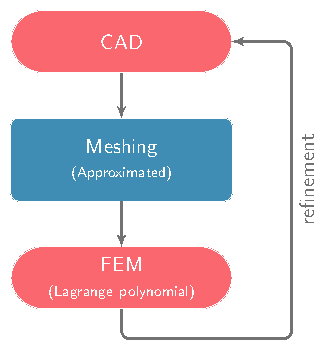
\includegraphics[scale=1.2]{flow-chart-fem}
		\caption{FEA workflow}
	\end{subfigure}
	\begin{subfigure}[b]{0.47\textwidth}
		\centering
		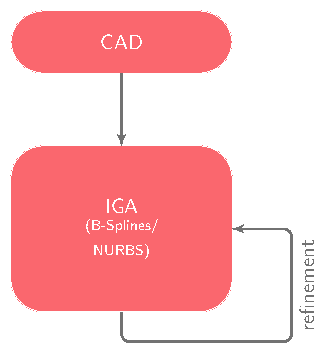
\includegraphics[scale=1.2]{flow-chart-iga}
		\caption{IGA workflow}
	\end{subfigure}
	\caption{A comparison of between classical finite element analysis workflow and isogeometric analysis workflow. FEA workflow: meshing and cleanup are required. Note that the meshing process does not preserve the original CAD geometry. IGA workflow: using the CAD model directly in the finite element analysis. }
	\label{fig:flow_chart}
\end{figure}

CAD models are often built from collections of non-uniform rational B-splines (NURBS). Adjacent NURBS patches often have inconsistent knot layouts, different parameterizations, and may not even be physically connected. Additionally, trimming curves~\cite{kim2009isogeometric, schmidt2012isogeometric} are often employed to further simplify the design process and to extend the range of objects that can be modeled by NURBS at the expense of further complicating the underlying parameterization of the object. While usually not an issue from a design perspective, these inconsistencies in the NURBS patch layout, including trimming, must be accommodated in the isogeometric model to achieve accurate simulation results. As shown in Figure~\ref{fig:geometries}, two primary approaches are often employed. First, the exact trimmed CAD model, shown in Figure~\ref{fig:geometries} in the middle, is used directly in the simulation~\cite{schmidt2012isogeometric}. To accomplish this requires additional algorithms for handling cut cells and the weak imposition of boundary conditions and may result in reduced solution accuracy and robustness. Second, the CAD model is reparameterized~\cite{xu2014high}, as shown in Figure~\ref{fig:geometries} on the right, into a watertight spline representation like multi-patch NURBS, subdivision surfaces~\cite{peters2008subdivision}, or T-splines~\cite{sederberg_t-splines_2003} which can then be used as a basis for analysis directly. The reparameterization process often results in more accurate and robust simulation results but is only semi-automatic using prevailing approaches. In both cases, existing techniques are primarily surface-based due to the predominance of surface-based CAD descriptions.

\begin{figure}[ht]
	\captionsetup[subfigure]{labelformat=empty, font = footnotesize}
	\centering
	\begin{subfigure}[b]{0.32\textwidth}
		\centering
		\includestandalone[scale=.7]{geometry}
		\caption{A geometry}
	\end{subfigure}
	\begin{subfigure}[b]{0.32\textwidth}
		\centering
		\includestandalone[scale=.7]{trimmed_geometry}
		\caption{Trimmed model}
	\end{subfigure}
	\begin{subfigure}[b]{0.32\textwidth}
		\centering
		\includestandalone[scale=.7]{reparameterized_geometry}
		\caption{Reparameterized model}
	\end{subfigure}
	\caption{A geometry and two modelling strategies: trimming and reparameterization.}
	\label{fig:geometries}
\end{figure}

From the analysis perspective, the main challenge for conducting finite element analysis over a geometry consisting of multiple spline patches is how to efficiently and accurately exchange information among different patches. In this dissertation, we focus on the \textit{dual mortar method}, which can robustly apply constraints over intersections of reparameterized multi-patch geometries.  

\section{State of the art}

Researchers in both the design and analysis communities have made significant progress in handling multi-patch NURBS models and the connections between adjacent patches. In this section, we present a brief review of patch coupling techniques developed in both communities. 
\subsection{Local refinable splines}

\begin{figure}[h]
    \centering
    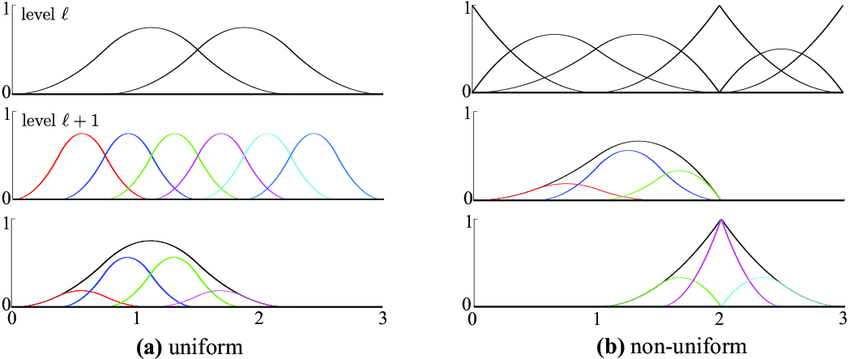
\includegraphics[width=.8\linewidth]{hierarchical-bsplines}
    \caption{Subdivision of B-spline basis functions: (a) Uniform, and (b) non-uniform B-spline basis functions are represented by linear combinations of refined basis functions~\cite{hennig2016bezier}.}\label{fig:hierarchical-bsplines}
\end{figure}

 In order to represent complex topologies, subdivision schemes (Figure.~\ref{fig:hierarchical-bsplines}) are widespread in geometry processing and computer graphics. Subdivision schemes allow for the construction of smooth spline bases over unstructured meshes. Among the most popular subdivision schems are the Catmull-Clark \cite{catmull_recursively_1978}, Doo-Sabin \cite{doo_behaviour_1978} and Loop's \cite{loop_smooth_1987} scheme. For isogeometric analysis, Wei \textit{et al.} \cite{wei_truncated_2015} introduced truncated hierarchical Catmull-Clark subdivion that can handle extraordinary nodes involved in complex topologies. Truncated hierarchical Catmull-Clark subdivion inherits the surface continuity of Catmull-Clark subdivision, namely $C^1$ continuity at extraordinary points and $C^2$ continuity elsewhere. Loop subdivision surfaces provide similar regularity properties as truncated hierarchical Catmull-Clark subdivion and have been applied to isogeometric analysis in \cite{kang_truncated_2016,pan_isogeometric_2015} to generate triangular meshes. One of the limitations in the implementation of subdivision meshes is that the basis function around the extraordinary point is composed of piecewise polynomial functions with an infinite number of segments, which leads to insufficient integration by Gauss quadrature. To deal with this issue, various quadrature rules and adaptive strategies have been examined in \cite{nguyen_comparative_2014} for the Poisson problem on the disk and in \cite{juttler_numerical_2016} for fourth order partial differential equations. \par

\begin{figure}[h]
    \centering
    \begin{subfigure}[b]{0.45\textwidth}
        \centering
        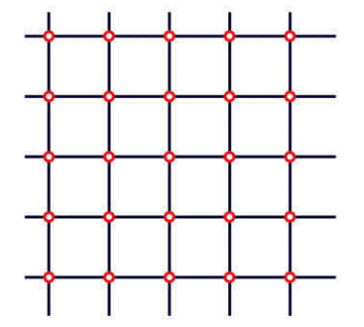
\includegraphics[width=\linewidth]{bspline-control-grid}
        \caption{B-splines}
    \end{subfigure}
    ~
    \begin{subfigure}[b]{0.45\textwidth}
        \centering
        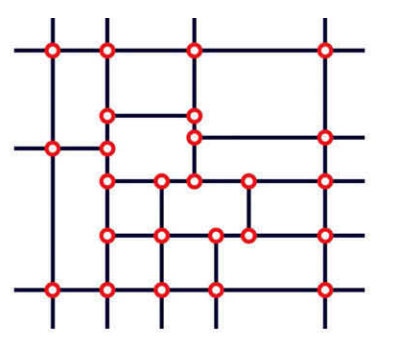
\includegraphics[width=\linewidth]{tspline-control-grid}
        \caption{T-splines}
    \end{subfigure}   
    \caption{Control points lie in a rectangular grid. (a) Topology of B-spline control grid. (b) Topology of T-spline
    control grid, the presence of T-junction control points is allowed~\cite{bazilevs_isogeometric_2010}.}\label{fig:Tspline-control-grid}
\end{figure}

\begin{figure}[h]
    \centering
    \begin{subfigure}[b]{0.45\textwidth}
        \centering
        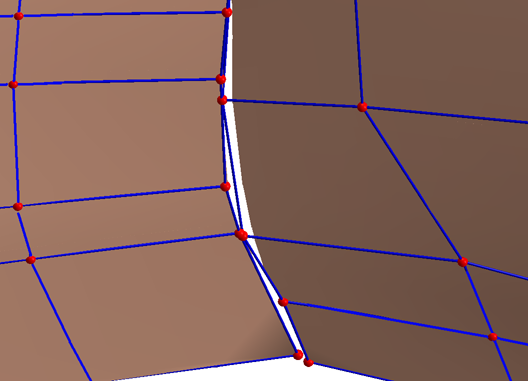
\includegraphics[width=\linewidth]{bspline-two-patch}
        \caption{B-splines}
    \end{subfigure}
    ~
    \begin{subfigure}[b]{0.45\textwidth}
        \centering
        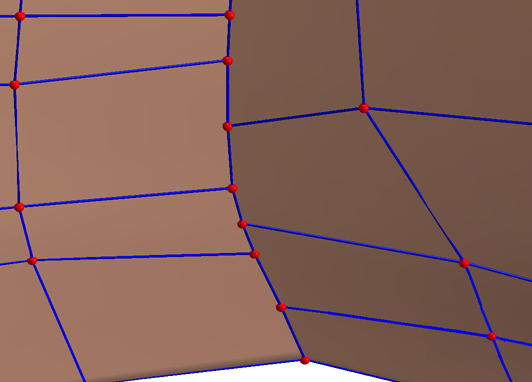
\includegraphics[width=\linewidth]{tspline-two-patch}
        \caption{T-splines}
    \end{subfigure}   
    \caption{A gap between two B-spline surfaces, fixed with a T-spline~\cite{sederberg_t-splines_2003}.}\label{fig:Tspline-two-patch}
\end{figure}

In 2003, Sederberg \textit{et al.} \cite{sederberg_t-splines_2003} introduced T-splines, which allow for the existence of T-junctions in the mesh, so that lines of control points need not traverse the entire mesh. Thus, local refinement can be realized by introducing T-junctions (see Figure.~\ref{fig:Tspline-control-grid}) around interested region. Since the concept of T-splines is a generalization of NURBS technology, it can also be used to merge NURBS surfaces that have different discretizaitons at the intersection (see Figure.~\ref{fig:Tspline-two-patch}). Due to the desirable features of T-splines, Bazilevs \textit{et al.} \cite{bazilevs_isogeometric_2010} explored this technology in isogeometric analysis, and numerical results demonstrated its potential for solving structural and fluid problems. By utilizing the B\'ezier extraction operator, a finite element data structure for T-splines \cite{scott_isogeometric_2011} were developed to ease the incorporation of T-splines into existing finite element codes. However, it has been proven \cite{buffa_linear_2010} that the original definition of T-splines is not sufficient to ensure the linear independence of the basis functions. To circumvent this issue, analysis suitable T-splines \cite{li_linear_2012} were developed by applying an additional constraint that no two orthogonal T-junction extensions are allowed to intersect. Subsequently, the mathematical properties of analysis suitable T-splines were studied in \cite{li_analysis-suitable_2013,xin_li_properties_2015}, and it has been sucessfully applied to the boundary element method \cite{scott2013isogeometric}. Meanwhile, an adaptive local h-refinement algorithm with T-splines and a local refinement of analysis-suitable T-splines were introduced by D\"{o}fel \textit{et al.} \cite{dorfel_adaptive_2010} and Scott \textit{et al.} \cite{scott_local_2012}, respectively. However, for both algorithm, the refined mesh is not as local as one would hope and this problem might be severe in 3D.\par

\subsection{Multi-patch geometrically continuous functions}

One of the advantages of isogeometric analysis is that it provides basis functions with high smoothness, \textit{i.e.} for $p$-th order splines, they enjoy up to $C^{p-1}$ continuity within a single patch. Thus, it is possible to directly discretize differential operators of order higher than 2. However, continuity higher than $C^0$ for multi-patch discretization imposes significant difficulties. The conception of geometric continuity is a well-known and highly useful concept in geometric design \cite{peters_chapter_2002, peters_joining_1992}. The parametric continuity requires both the smoothness of the geometry and its parameterization, whileas the geometric continuity only requires the smoothness of the geometry. Hence, the geometric continuity of order $s$ ($G^s$ continuity) is a weaker continuity constraint as compared to $C^s$ parametric continuity. Bercovier \textit{et al.} \cite{bercovier_smooth_2014} has shown that for multi B\'ezier patches over an unstructured quadrilateral mesh, as long as the order of polynomial is high enough, there always exists the minimal determining set for a $G^1$ continuity construction. Moreover, the resulting basis functions do not contain subdivisions around extraordinary vetices.\par

The case of $G^1$ continuous functions on bilinearly parametrized two-patch B-spline domains was considered by Kapl \textit{et al.} \cite{kapl_isogeometric_2015}, where the $C^1$ basis functions are constructed and analyzed by numerical tests. It is shown that the space dimensionality heavily depends on the parameterization of two bilinear patch, and optimal convergence is observed on the biharmonic problem. However, over-constrained $C^1$ isogeometric spaces that cause sub-optimal convergence are also observed for certain configurations (\textit{e.g.} two-patch non-bilinear parameterizations and $C^{p-1}$ continuity within the patches for $p$-th order spline space). A theoretical analysis of the cause of this so-called $C^1$ locking phenomenon is provided in \cite{collin_analysis-suitable_2016}, where the analysis-suitable $G^1$ geometry parameterization that allows for optimal approximation of $C^1$ isogeometric spaces, is identified and verified by numerical examples. Kapl \textit{et al.} extended the construction of $G^1$ continuous functions to bilinearly parameterized multi-patch domains in \cite{kapl_isogeometric_2017}, where the simple explicit formulas for spline coefficients of $C^1$ basis function are derived and nested $C^1$ isogeometric spaces are generated. Recently, Kapl \textit{et al.} \cite{kapl_space_2017,kapl_space_nodate} explored the construction of $C^2$ isogeometric functions on multi-patch geometries and utilized the $C^2$ isogeometric spaces for $6$-th order PDE.\par

Although the geometrically continuous functions circumvent the use of subdivisions for domains with extraordinary vertices, the requirement of $C^0$ parameterization averts local mesh refinement, and lower continuity is required to avoid $C^1$ locking effect. Thus, its implementation can be complex and it may not be a potential candidate for analysis in more general situations.\par

\subsection{Variational approaches}

From the analysis perspective, the pointwise satisfaction of continuity constraints between adjacent patches is often unnecessarily rigorous. A reasonable approximation can be achieved even if these constraints are applied in a variational setting. The Lagrange multiplier method is a general framework which can be used to apply constraints to variational problems. In the context of isogeometric analysis, various types of Lagrange multiplier approaches have been applied to problems in solids~\cite{hesch_isogeometric_2012, seitz2016isogeometric} and fluids~\cite{bazilevs2012isogeometric}. While general in applicability, the solvability and optimality of the Lagrange multiplier method is significantly influenced by the \textit{inf-sup} condition~\cite{babuvska1973finite,boffi_mixed_2013}. In the context of domain coupling, to satisfy the \textit{inf-sup} condition, special modifications are needed when building the Lagrange multiplier space to ensure stability (see Figure~\ref{fig:mortar_basis}). This has been further studied in~\cite{bernardi_basics_2005, bernardi_domain_1993, belgacem_mortar_1998, barbosa1991finite} for finite element analysis and in~\cite{brivadis_isogeometric_2015} for isogeometric analysis. \par

Whereas the Lagrange multiplier method applies continuity constraint by Lagrange multipier, leading to a saddle point problem, the mortar method, first introduced by Bernardi~\cite{bernardi_domain_1993}, considers a constrained solution space and gives rise to a positive definite variational problem. Wohlmuth~\cite{wohlmuth2000mortar} used dual basis functions to discretize the Lagrange multiplier spaces, which further simplifies the mortar formulation. Dual basis functions for the piecewise linear elements are illustrated in Figure~\ref{fig:mortar_basis}. A dual mortar method for isogeometric analysis was first developed by Seitz et al.~\cite{seitz_isogeometric_2016}. \par

Applying constraints by the Lagrange multiplier method leads to a saddle point problem, of which the discrete Lagrange multiplier basis functions cannot be chosen independently of that of the primal variable and special treatment is required to ensure the solvability and optimality of the discretized system. The stiffness matrix for the discrete problem arising from the Lagrangian multiplier method always contains both positive and negative eigenvalues, for which iterative methods are known to be less efficient than for symmetric positive definite systems. The perturbed Lagrangian method alleviates these issues by appending a weighted quadratic penalty term to the energy functional. The main drawback of the perturbed Lagrangian method is the inconsistency with the original problem. It has been utilized in \cite{simo1985perturbed} for contact problems and \cite{dornisch2011boundary, apostolatos2015domain} for domain decomposition problems in the isogeometric analysis framework.\par

To fully circumvent the inf-sup condition for imposing Dirichlet boundary conditions by Lagrange multiplier, Barbosa et. al. \cite{barbosa1991finite} added a new penalty like term to the energy functional to enhance the stability. Unlike perturbed Lagrangian methods where the penalty term is inconsistent with the original problem, the new term proposed by Barbosa maintains the consistency. It has been demonstrated that there is a close connection with the stablized Lagrange multiplier method and Nitsche's method in the context of setting the Dirichlet boundary conditions \cite{stenberg1995some} and in the context of domain decomposition \cite{hansbo2005lagrange, hansbo_nitsches_2005, juntunen2015connection}. Tur et. al. \cite{tur2015modified} utilized this method to solve both small and large deformation contact problems and obtained optimal convergence rates for linear elements. To our knowledge, this method has not been applied in the isogeometric analysis framework yet. \par

The discontinuous Galerkin method (or Nitsche's method) was introduced in 1971 \cite{nitsche_uber_1971} for handling Dirichlet boundary conditions in the weak sense. The discontinuous Galerkin method resembles a mesh-dependent penalty method. Unlike the standard penalty method, which is not consistent unless the penalty coefficient goes to infinity, the discontinuous Galerkin method is consistent with the original problem. Moreover, no additional unknown (Lagrange multiplier) is needed and no discrete inf-sup condition must be fulfilled, contrarily to mixed methods. Meanwhile, additional terms are added into the weak form to ensure the ellipticity of the problem. The discontinuous Galerkin method has been widely studied in various aspects, including imposing boundary conditions \cite{hansbo_nitsches_2005}, domain decomposition \cite{becker_finite_2003} and contact problems \cite{chouly_symmetric_2015}. In the field of the isogeometric analysis, the discontinuous Galerkin method has been utilized to impose Dirichlet boundary conditions for trimmed spline meshes \cite{embar_imposing_2010}. The first article discussing the discontinuous Galerkin method based domain decomposition strategy was written by Apostolatos \textit{et al.} \cite{apostolatos_nitsche-type_2014}. Nguyen \textit{et al.} extended it to three-dimensional problems in \cite{nguyen_nitsches_2014}. Guo \textit{et al.} \cite{guo_nitsches_2015} proposed a Nitsche's method for coupling Kirchhoff-Love NURBS shell patches.\par

\begin{figure}
  \centering
  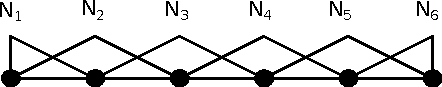
\includegraphics[width=.7\linewidth]{original_basis}\\
  \vspace{1em}
  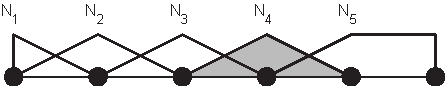
\includegraphics[width=.7\linewidth]{mortar_basis}\\
  \vspace{1em}
  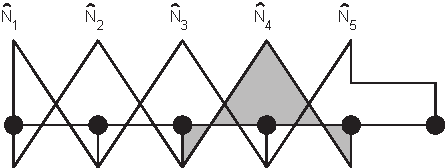
\includegraphics[width=.7\linewidth]{dual_mortar_basis}
  \caption{Lagrange multiplier basis functions for the piecewise linear elements, top: original piecewise linear basis, middle: piecewise linear basis with modification at the right end, bottom: dual basis functions for the piecewise linear elements, modification at the right end (Courtesy of Zienkiewicz~\cite{zienkiewicz1977finite}).}\label{fig:mortar_basis}
\end{figure}

\section{Research contributions}

In this dissertation, the dual mortar framework for most prevailing higher-order partial differential equations (including biharmonic problems, Cahn-Hilliard problems and Kirchhoff-Love shell problems) are developed. The primary contributions of this dissertation are:
\begin{itemize}
    \item Formulation and implementation of an isogeometric B\'ezier dual mortar method for the biharmonic problem on multi-patch domains. The formulation leads to an efficient construction of a sparse constrained linear system. We prove the well-posedness of the formulation and specify requirements to achieve optimal convergence. 
    \item Development of the enriched \Bezier dual basis. The enriched \Bezier dual basis functions are constructed via a quadrature-free algorithm and can reproduce polynomials up to a given degree. 
    \item Formulation and implementation of an isogeometric \Bezier dual mortar method for the Kirchhoff-Love shell problem on multi-patch domains. 
    \item Extension of \Bezier dual basis functions to alleviate transverse shear locking in Timoshenko beams and volumetric locking in nearly compressible linear elasticity. Based on the different interpretation of the $\bar{B}$ formulation, we develop two formulations for locking problems.
    \item An isogeometric analysis code in C++ is developed. Eigen library~\cite{eigenweb} is adopted as the primary linear solver. The assembly routine is multi-threaded by the thread module in the Standard Template Library (STL). This code is capable of handling nonlinear dyanmic problems with higher mesh resolution. 
\end{itemize}

\section{Organization of the dissertation}

The remainder of this thesis is structured as follows: Chapter~\ref{chp:chapter2} provides an overview of isogeometric analysis, e.g. the formulation of B-splines and NURBS, knot insertion and degree elevation algorithms. In addition, the concepts of \Bezier extraction/projection and dual basis functions are explained. In Chapter~\ref{chp:chapter3} the \Bezier dual mortar method for the biharmonic problem is theoretically and numerically studied. The optimality of the proposed formulation requires the \textit{inf-sup} stable as well as a suitable approximation property for the Lagrange multiplier space. However, numerical studies indicate that \Bezier dual basis fails to provide adequate approximation, leading to sub-optimal convergence results. In Chapter~\ref{chp:chapter4}, we investigate all factors that influence the approximation of basis functions and develop the enriched \Bezier dual basis. The enriched \Bezier dual basis, constructed via a quadrature-free algorithm, possesses the polynomial reproduction ability and compact support. The accuracy and robustness of the enriched \Bezier dual basis is thoroughly tested by various $2^\text{nd}$ and $4^\text{th}$ order problems. In Chapter~\ref{chp:chapter5}, the \Bezier dual mortar method for the Kirchhoff-Love shell problem is presented. The formulation is based on a dual mortar compatible constraint and handles both smooth shell coupling problem as well as kinked shell coupling problem. The enriched \Bezier dual basis is adopted as discretized Lagrange multipliers, leading to a sparse linear system. Several linear and nonlinear benchmark problems verify the accuracy and robustness of this approach. In Chapter~\ref{chp:chapter6}, the application of \Bezier dual basis is extended to alleviate transverse shear locking in Timoshenko beams and volumetric locking in nearly compressible linear elasticity without populating the stiffness matrix. Finally, conclusions and directions for future work are given in Chapter~\ref{chp:chapter7}.
% \chapter{Preliminaries}
\label{chp:chapter2}
\graphicspath{{figures/}{figures/chapter2/}}
\pgfplotsset{
    table/search path={{figures/chapter2/data},{data}},
}

Isogeometric analysis (IGA), introduced by Hughes et al. \cite{HUGHES20054135}, adopts the spline basis, which underlies the CAD geometry, as the basis for analysis. Of particular importance is the positive impact of smoothness on numerical solutions, where, in many application domains, IGA outperforms classical finite elements~\cite{cottrell2009isogeometric,cottrell_studies_2007,cottrell2006isogeometric,hughes_duality_2008,bazilevs_isogeometric_2010,evans_n-widths_2009}.

In this chapter, a brief overview of spline basis functions that are most commonly used in Isogeometric Analysis are given in~\ref{sec:spline_overview}. In~\ref{sec:geometric_algorithms}, we review some of the most popular algorithms in manipulating splines including \Bezier extraction and \Bezier projection. Dual basis serves as the main research tool for this thesis. The concept of dual basis functions is also introduced in~\ref{sec:dual_basis}.

\section{Splines}\label{sec:spline_overview}

\subsection{The univariate Bernstein basis}

The $i^{\text{th}}$ univariate Bernstein basis function of degree $p$ on the unit interval $\left[ 0,1 \right]$ is defined by
\begin{equation}
    B_i^p(\xi) = \binom {p}{i}\xi^i(1-\xi)^{p-i}
\end{equation}
where the binomial coefficient $\binom {p}{i}=\dfrac{p!}{i!(p-i)!}$, $0\leq{i}\leq{p}$. The polynomial degree superscript will be omitted when unnecessary. Matrix-vector notation will be used throughout, with bold fonts indicating matrices and vectors, e.g. the vector form of a set of Bernstein basis functions is denoted by
\begin{equation}
    \mathbf{B}^p(\xi)=
    \begin{bmatrix}
        B_0^p(\xi) \\
        B_1^p(\xi) \\
        \vdots     \\
        B_p^p(\xi)
    \end{bmatrix}.
\end{equation}
The Bernstein basis of degree $p$ spans the space of polynomials of degree $p$. The Gramian matrix $\mathbf{G}^p = [G_{i,j}^p]$ can be computed by
\begin{equation}
    G_{i,j}^p=\int_0^1B_i^p(\xi) B_j^p(\xi)d\xi,\qquad{i,j\in\left\{0,1,\dots, p\right\}}.\label{eq:gramian_bernstein}
\end{equation}
Eq.~\eqref{eq:gramian_bernstein} can be evaluated in closed form (see~\cite{farouki1988algorithms}) as
\begin{equation}
    G_{i,j}^p = \frac{\binom {p}{i}\binom {p}{j}}{(2p+1)\binom {2p}{i+j}}\label{eq:gramian_bernstein_closed_form}
\end{equation}
and its inverse (see~\cite{juttler1998dual}) as
\begin{equation}
    [G_{i,j}^p]^{-1} = \frac{(-1)^{i+j}}{\binom {p}{i}\binom {p}{j}}\sum_{k=0}^{\min(i,j)}\binom{p+k+1}{p-i}\binom{p-k}{p-i}\binom{p+k+1}{p-j}\binom{p-k}{p-j}.\label{eq:inverse_gramian_bernstein_closed_form}
\end{equation}
A Bernstein basis defined over an arbitrary interval $\left[\xi_\alpha,\xi_\beta\right]$ can be evaluated from
\begin{equation}
    B_i^p(\frac{\xi-\xi_\alpha}{\xi_\beta-\xi_\alpha}),\qquad \xi\in\left[\xi_\alpha,\xi_\beta\right].
\end{equation}
The corresponding Gramian and inverse can be obtained by multiplying and dividing the matrices in Eq.~\eqref{eq:gramian_bernstein_closed_form} and Eq.~\eqref{eq:inverse_gramian_bernstein_closed_form} by the scaling factor $(\xi_\beta-\xi_\alpha)$, respectively. For the sake of simplicity, we use the same symbols to represent the Bernstein basis defined on different intervals. A closed form expression for the $L^2$ inner product between the Bernstein basis $B_i^p(\xi)$ and polynomial $\xi^j$ is given by
\begin{equation}
    \int_0^1 B_i^p (\xi) \xi^j d\xi = \binom{p}{i} \frac{(i+j)! (p-i)!}{(p+j+1)!}.\label{eq:inner_product_bernstein_polynomial}
\end{equation}

Bernstein basis possess the following properties:
\begin{itemize}
    \item Nonnegativity: $B_i^p(\xi)\geq 0$ for all $i$, $p$, and $0\leq\xi\leq 1$;
    \item Partition of unity: $\sum_{i=0}^pB_i^p(\xi)=1$, for all $0\leq\xi\leq 1$;
    \item Interpolatory at the ends: $B_0^p(0)=B_p^p(1)=1$.
\end{itemize}
% Given a set of control points $\left\{\mathbf{P}_i\right\}_{i=0}^p$, the corresponding \Bezier curve is defined by:
% \begin{equation}
%     \mathbf{C}(\xi) = \sum_{i=1}^p\mathbf{P}_i B_i^p(\xi).
% \end{equation}

However, the global support of the Bernstein basis makes it impossible to locally edit a \Bezier curve, which is a urgent requirement for geometry modeling. This problem can be overcome by using B-splines.

\subsection{The univariate B-spline basis}

A set of univariate B-spline basis functions of degree $p$ can be uniquely defined by a non-decreasing knot vector $\mathbf{\Xi}=\left\{\xi_i\right\}_{i=0}^{n+p}$, where $n$ is the number of B-spline basis functions. In this work, we only use open knot vectors, i.e., $\xi_0=\xi_1=\dots=\xi_{p}$ and $\xi_{n}=\xi_{n+1}=\dots=\xi_{n+p}$ defined over the interval $\left[0,1\right]$. The value of the $i^{\text{th}}$ B-spline basis function is recursively defined using the Cox-de Boor formula~\cite{piegl2012nurbs}
\begin{align}
    N_{i}^0(\xi) & =\begin{cases}1 & \xi_i\leq{\xi}\leq{\xi_{i+1}}\\0 & \text{otherwise} \end{cases}                                                                                          \\
    N_{i}^p(\xi) & =\frac{\xi-\xi_i}{\xi_{i+p}-\xi_i}N_{i}^{p-1}(\xi)+\frac{\xi_{i+p+1}-\xi}{\xi_{i+p+1}-\xi_{i+1}}N_{i+1}^{p-1}(\xi).
\end{align}

In addition to the properties of Bernstein basis, B-splines also possess:
\begin{itemize}
    \item Compact support: $\supp{N_{i}^p}\subset \left[\xi_i,\xi_{i+p+1}\right]$.
\end{itemize}
This feature is crucial for both geometry modeling and finite element analysis. In modeling, it allows the changing in a localized region while keeping other parts unchanges. In finite element analysis, it ensures the sparse structure of the discretized linear system.

\begin{figure}[ht]
    \center
    \begin{subfigure}[t]{\linewidth}
        \center
        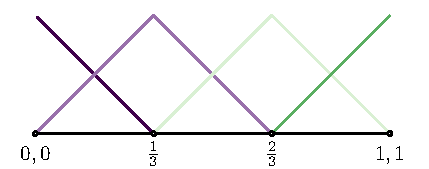
\includegraphics[scale=1.2]{p=1_space}
    \end{subfigure}
    \begin{subfigure}[t]{\linewidth}
        \center
        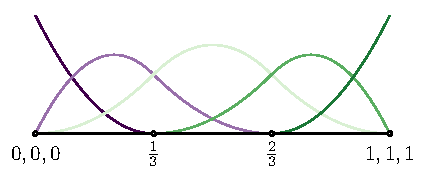
\includegraphics[scale=1.2]{p=2_space}
    \end{subfigure}
    \caption[B-spline basis functions of different degrees.]{B-spline basis functions of different degrees. Top: linear spline basis functions defined by $\left\{0,0,1/3,2/3,1,1\right\}$. Bottom: quadratic spline basis functions defined by $\left\{0,0,0,1/3,2/3,1,1,1\right\}$.}\label{fig:spline_basis}
\end{figure}

B-splines of different degrees are shown in Figure~\ref{fig:spline_basis}. As can be seen, linear B-spline basis functions are identical to the classic hat functions that widely used in finite element analysis. Compared with quadratic Lagrange polynomials in Figure~\ref{fig:lagrange_polynomial}, quadratic B-splines are smoother across each mesh grids. Indeed, B-splines of degree $p$ have up to $p-1$ continuous derivatives. The inter-element continuity can be manipulated by repeating knots. In general, basis functions at knot of multiplicity $m$ are $C^{p-m}$ continuity.

\begin{figure}[ht]
    \center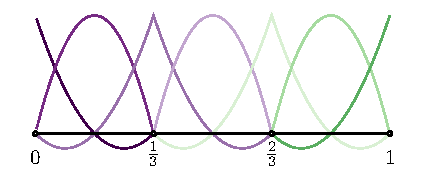
\includegraphics[scale=1.2]{p=2_space_2}
    \caption{Quadratic Lagrange polynomials defined on the same mesh grid as the splines in Figure~\ref{fig:spline_basis}.}\label{fig:lagrange_polynomial}
\end{figure}


A $d$-dimensional B-spline curve $\mathbf{S}(\xi)\in{\R^d}$ can then be defined as
\begin{equation}
    \mathbf{S}(\xi)=\sum_A N_{A,p}(\xi)\mathbf{P}_A
\end{equation}
where $\mathbf{P}_A=(p_A^1,p_A^2,\ldots,p_A^d)^T$ is a $d$-dimensional control point. An example of a B-spline curve is illustrated in Figure~\ref{fig:b-spline_and_geometry}.

\begin{figure}[ht]
    \center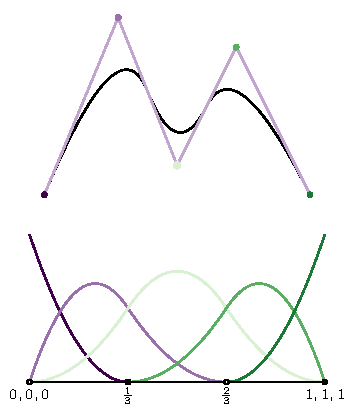
\includegraphics[scale=1.3]{geometry}
    \caption{A B-spline piecewise quadratic curve in $\R^2$ and the corresponding B-spline basis.}\label{fig:b-spline_and_geometry}
\end{figure}

\FloatBarrier
\subsection{The univariate NURBS basis}

B-splines can be used to represent piecewise polynomial functions but are not capable of representing conic sections (e.g. circles, ellipses and hyperbolas). NURBS(Non-Uniform Rational B-Spline) overcome this shortcoming.  A NURBS basis function can be written as
\begin{equation}
    R_{A,p}(\xi)=\dfrac{N_{A,p}(\xi)w_A}{W{(\xi)}}
\end{equation}
where $w_A$ is called a weight and
\begin{align}
    \label{eq:weight}
    W(\xi)=\sum_{A} N_{A,p}(\xi)w_A
\end{align}
is called the weight function. A $d$-dimensional rational curve $\mathbf{S}(\xi)\in{\R^d}$ can then be defined as
\begin{equation}
    \mathbf{S}(\xi)=\sum_A R_{A,p}(\xi)\mathbf{P}_A.
\end{equation}
It is often more convenient to represent the $d$-dimensional NURBS in a $(d+1)$-dimensional homogeneous space by defining $\mathbf{P}_A^w=(p_A^1w_A,p_A^2w_A,\ldots,p_A^dw_A,w_A)^T$ and the corresponding $(d+1)$-dimensional B-spline curve as
\begin{align}
    \mathbf{S}^w(\xi) & =\sum_A N_{A,p}(\xi)\mathbf{P}_A^w
\end{align}
such that each component of $\mathbf{S}^w$ can be written as
\begin{align}
    S_i(\xi) & =\dfrac{{S}_i^w(\xi)}{{S}_{d+1}^w(\xi)}.
\end{align}
In the homogeneous form, NURBS can be manipulated with standard B-spline algorithms.

\subsection{The multivariate spline basis}

In higher dimensions, Bernstein, B-spline, and NURBS basis functions are formed by the Kronecker product of univariate basis functions. For example, two-dimensional B-spline basis functions of degree $\mathbf{p}=(p_\xi, p_\eta)$ are defined by
\begin{equation}
    \mathbf{N}^\mathbf{p}(\xi,\eta)=\mathbf{N}^{p_\xi}(\xi)\otimes\mathbf{N}^{p_\eta}(\eta)
\end{equation}
where $\mathbf{N}^{p_\xi}(\xi)$ and $\mathbf{N}^{p_\eta}(\eta)$ are vectors of basis functions in the $\xi$ and $\eta$ directions, respectively. A particular multivariate basis function can be written as
\begin{equation}
    {N}_{A(i,j)}^\mathbf{p}(\xi,\eta)={N}_{i,p_\xi}(\xi){N}_{j,p_\eta}(\eta)
\end{equation}
where the index mapping is defined as
\begin{equation}
    A(i,j)=n_\eta{i}+j.
\end{equation}
The integer $n_\eta$ is the number of basis functions in $\eta$ direction. In three-dimensional space, a set of basis functions can be constructed by the Kronecker product between two-dimensional basis functions and univariate basis functions.

\section{Geometric Algorithms}\label{sec:geometric_algorithms}

\subsection{Knot insertion}

The knot insertion algorithm ensures the insertion of one or multiple knots into a knot vector $\mathbf{\Xi}$ without changing the shape and parameterization of the curve. It allows us to conduct \textit{h}-refinement (subdividing elements into smaller ones without changing the type of basis functions used) in the context of Isogeometric Analysis. The detailed algorithm of knot insertion can be found in~\cite{piegl2012nurbs}.

An example of knot insertion of the B-spline curve in Figure~\ref{fig:b-spline_and_geometry} is illustrated in Figure~\ref{fig:b-spline_h_refine}. A set of knots $\left\{\frac{1}{6}, \frac{1}{2}, \frac{5}{6}\right\}$ are inserted into the original knot vector $\mathbf{\Xi}=\left\{0,0,0,1/3,2/3,1,1,1\right\}$.  The inserted curve remains geometrically and parametrically identical to the original curve. Meanwhile, knot spans $[ \xi_i,\xi_{i+1} )$ are splitted into smaller ones.

\begin{figure}[ht]
    \center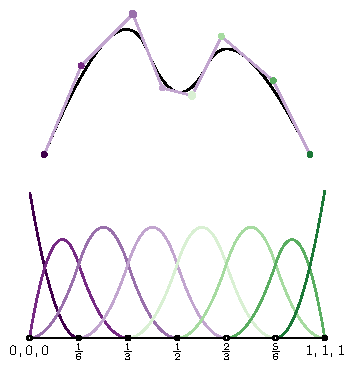
\includegraphics[scale=1.3]{h_refine}
    \caption{Knot insertion for the curve in Figure~\ref{fig:b-spline_and_geometry}. The inserted curve is geometrically and parametrically identical to the original curve.}\label{fig:b-spline_h_refine}
\end{figure}

\subsection{Degree elevation}

The degree elevation algorithm increases the polynomial degree of each B-spline basis functions while preserves the geometry and parameterization of the curve. It allows us to conduct \textit{p}-refinement (increasing the degree of basis functions without changing the number of element used) in the context of Isogemetric Analysis. The detailed algorithm of degree elevation can be found in~\cite{piegl2012nurbs}.

An example of degree elevation of the B-spline curve in Figure~\ref{fig:b-spline_and_geometry} is illustrated in Figure~\ref{fig:b-spline_p_refine}, where the original quadratic spline curve is elevated to cubic and the shape remains unchanged. Recalling that the basis is $C^{p-m}$ continuous at a knot of multiplicity $m$, it is clear that, to preserve the inter-element continuity, the multiplicity of each knots must be increased as the increase of the polynomial degree. In Figure~\ref{fig:b-spline_p_refine}, the multiplicity each knot is increased by one.

\begin{figure}[ht]
    \center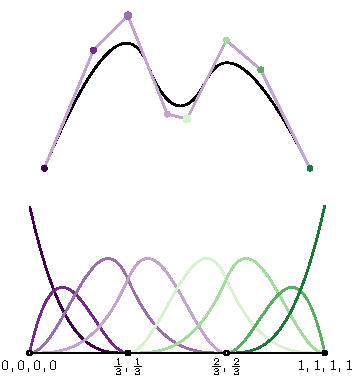
\includegraphics[scale=1.3]{p_refine}
    \caption{Degree elevation for the curve in Figure~\ref{fig:b-spline_and_geometry}. The degree elevated curve is geometrically and parametrically identical to the original curve.}\label{fig:b-spline_p_refine}
\end{figure}

\subsection{\Bezier extration}

\Bezier extraction is a technique that is often used to facilitate the incorporation of isogeometric analysis into existing finite element codes~\cite{borden2011isogeometric,scott2011isogeometric}. \Bezier extraction defines an injection that maps a space spanned by B-spline basis to a space spanned by piecewise Bernstein basis. \Bezier extraction is accomplished by repeating all interior knots of a knot vector until they have a multiplicity equal to $p+1$. The interior knots repeating process defines a linear operator $\mathbf{C}$ (see~\cite{borden2011isogeometric}) such that
\begin{equation}
    \mathbf{N}(\xi)=\mathbf{C}\mathbf{B}(\xi).
\end{equation}
The localization of $\mathbf{C}$ to an element domain produces the element extraction operator $\mathbf{C}^e$.
Given control points $\mathbf{P}^e$, the corresponding B\'ezier control points $\mathbf{Q}^e$ can be computed directly as
\begin{equation}
    \mathbf{Q}^e=(\mathbf{C}^e)^T\mathbf{P}^e.
\end{equation}
A graphical depiction of B\'{e}zier extraction over an element is shown in Figure~\ref{fig:element_extraction_projection}.

\begin{figure}
    \centering
    \begin{subfigure}{\linewidth}
        \center
        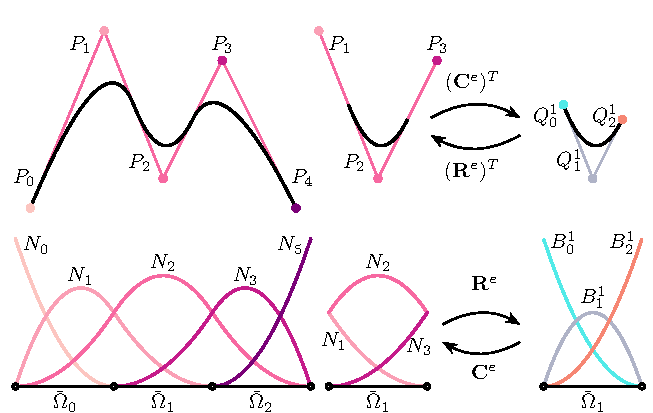
\includegraphics[width=.7\linewidth]{elements_global.pdf}
        \caption{}\label{fig:element_extraction_projection}
    \end{subfigure}
    \begin{subfigure}{\linewidth}
        \center
        \includestandalone[scale = .8]{bezier_extraction_demo}
        \caption{}\label{fig:bezier_extraction_process}
    \end{subfigure}
    \caption{Illustration of \Bezier extraction and projection in one dimension for a B-spline of degree 2 and knot vector $\left\{0,0,0,1/3/2/3,1,1,1\right\}$. (a) The element extraction and projection for the second element. (b) \Bezier extraction over the entire domain.}
\end{figure}

It is possible to view \Bezier projection as a global assembly procedure. The B-spline basis vector $\mathbf{N}$ of dimension $n_N$ can be represented by a set of Bernstein basis functions $\mathbf{B}$ of dimension $n_B$ defined on each element as
\begin{equation}
	\mathbf{N} = \mathbf{A}^T\mathbf{C}\mathbf{B},
\end{equation}
where $\mathbf{C}$ is a block diagonal matrix with \Bezier element extraction operators on the diagonal and the rectangular assembly operator $\mathbf{A}$ is the permutation matrix that maps local element degrees of freedom to global degrees of freedom. The assembly operator $\mathbf{A}$ satisfies the following properties:
\begin{itemize}
	\item Each row of $\mathbf{A}$ contains a single unity-valued entry; all other entries are zero.
	\item Each column of $\mathbf{A}$ contains at most $p+1$ unity-valued entries; all other entries are zero.
	\item Compact support. The non-zero entries can be associated to no more than $p+1$ consecutive elements.
	\item If we consider the column vectors $\mathbf{A}_i$ of $\mathbf{A}$, the space $\spn\left\{\mathbf{A}_i\right\}_{i=0}^{n_N-1}$ is an $n_N$ dimensional subspace of $\mathbb{R}^{n_B}$ and $\left\{\mathbf{A}_i\right\}_{i=0}^{n_N-1}$ are orthogonal, i.e.
	      \begin{equation}
		      \mathbf{A}_i\cdot\mathbf{A}_j\neq{}0\iff{i=j}.
	      \end{equation}
\end{itemize}

The \Bezier extraction process for the quadratic B-spline basis defined by the knot vector $\{0,0,0,1/3,2/3,1,1,1\}$ is shown in Fig.~\ref{fig:bezier_extraction_process}. The assembly operator $\mathbf{A}$ for this example is given by
\begin{equation}\label{eq:assembly_matrix}
	\mathbf{A} =
	\begin{blockarray}{cccccc}
		N_0 & N_1  & N_2  & N_3  & N_4 \\
		\begin{block}{[ccccc]c}
			1 & \hfsetfillcolor{hred!10}\hfsetbordercolor{hred}\tikzmarkin{a}(0.1,-0.1)(-0.1,0.35)0 & 0 & 0 & 0 & N_0^0 \\
			0 & 1 & 0 & 0 & 0 & N_1^0 \\
			0 & 0 & 1 & 0 & 0 & N_2^0 \\
			0 & 1 & 0 & 0 & 0 & N_0^1 \\
			0 & 0 & 1 & 0 & 0 & N_1^1 \\
			0 & 0 & 0\tikzmarkend{a} & 1 & 0 & N_2^1 \\
			0 & 0 & 1 & 0 & 0 & N_0^2 \\
			0 & 0 & 0 & 1 & 0 & N_1^2 \\
			0 & 0 & 0 & 0 & 1 & N_2^2 \\
		\end{block}
	\end{blockarray},
\end{equation}
where the highlighted submatrix is the restriction of $\mathbf{A}$ onto elements $\Omega_0$ and $\Omega_1$, and onto the B-spline basis functions $N_1$ and $N_2$.

\subsection{B\'ezier projection}
\label{sec:bproject}

B\'{e}zier projection can be viewed as the inverse of extraction~\cite{thomas_bezier_2015}. It defines an surjection that maps a space spanned by  piecewise Bernstein basis onto a space spanned by B-spline basis. B\'ezier projection uses an element reconstruction operator $\mathbf{R}^e\equiv(\mathbf{C}^e)^{-1}$ such that the global control point values, corresponding to those basis functions defined over the support of an element $e$, can be determined directly from \Bezier control values as
\begin{equation}
    \mathbf{P}^e=(\mathbf{R}^e)^T\mathbf{Q}^e
\end{equation}
where $\mathbf{Q}^e$ is any field in B\'ezier form. The action of the element reconstruction operator is depicted graphically in Figure~\ref{fig:element_extraction_projection}. For example, given any function $u \in L^2$, we can compute $\mathbf{Q}^e$ as
\begin{equation}
    \mathbf{Q}^e=(\mathbf{G}^e)^{-1}\mathbf{F}^e
    \label{eq:element-Qi}
\end{equation}
where $\mathbf{G}^e$ is the Gramian matrix corresponding to the Bernstein basis with components
\begin{align}
    {G}_{ij}^e & = \int_{\Omega^e} B^e_i B^e_j \, d\Omega =\langle{B^e_{i},B^e_{j}}\rangle_{\Omega^e}\label{eq:element_gramian}
\end{align}
and
\begin{align}
    {F}^e_i & =  \int_{\Omega^e} B^e_i u \, d\Omega = \langle{B^e_{i,},u}\rangle_{\Omega^e}.
\end{align}
Note that efficiency gains can be had at the expense of accuracy by instead performing the integration in the parametric domain of the element~\cite{thomas_bezier_2015}.

The element-wise projection produces one control value for each element in the support of the function.  These values must be combined in order to provide the final control value.  A core component of the B\'ezier projection algorithm is the definition of an appropriate averaging operation. The process of computing the weights is illustrated in Figure~\ref{fig:weights}. A weighted average of the values is computed using the weighting
\begin{equation}\label{eq:Bezier_weight}
    \omega_a^e=\dfrac{\int_{\Omega^e} N_{a}^e \, d\Omega}{\int_{\Omega^A} N_{A(e,a)} \, d\Omega}
\end{equation}
where $\Omega^e$ corresponds to the physical domain of element $e$, $A(e,a)$ is a mapping from a local nodal index $a$ defined over element $e$ to a corresponding global node index $A$, and $\Omega^A$ corresponds to the physical support of $N_A$. The final averaged global control point is then calculated as
\begin{equation}
    P_A=\sum_{\Omega^e\in \Omega^A } \omega_{A(e,a)} P_{A(e,a)}.
\end{equation}
B\'ezier projection onto NURBS functions can be defined in an analogous manner~\cite{thomas_bezier_2015}.

The individual steps comprising the \Bezier projection algorithm are
illustrated in Figure~\ref{fig:loc-proj-example} where
the curve defined by $\vec{f}(t)=\left( \frac{t}{3}
    \right)^{3/2}\vec{e}_1+\frac{1}{10}\sin (\pi t )\,\vec{e}_2$,
$t\in[0,3]$ is projected onto the quadratic B-spline basis defined by
the knot vector $\left\{0,0,0,\frac{1}{3},\frac{2}{3},1,1,1\right\}$. For this example,
the algorithm proceeds as follows:

\begin{description}

    \item{Step 1:} The function $\mathbf{f}$ is projected onto the Bernstein basis of each element. This results in a set of
          \Bezier coefficients that define an approximation to $\mathbf{f}$.
          The \Bezier coefficients are indicated in part (1) of Figure~\ref{fig:loc-proj-example} by
          square markers that have been colored to match the corresponding
          element. Each \Bezier segment is discontinuous.

    \item{Step 2:} The element reconstruction operator $\mathbf{R}^e$ is used to convert the
          \Bezier control points into spline control points associated with the
          basis function segments over each element.
          The new control points are marked with inverted triangles and
          again colored to indicate the element with which the control point is
          associated. The control points occur in clusters.
          The clusters of control points represent the contributions from
          multiple elements to a single spline basis function control point.

    \item{Step 3:} Each cluster of control points is averaged to obtain a
          single control point by weighting each point in the cluster according
          to the weighting given in (\ref{eq:Bezier_weight}). The resulting control
          points are shown as circles with the relative contribution from each
          element to each control point indicated by the colored fraction of the
          control point marker. Colors in Figures~\ref{fig:weights} and~\ref{fig:loc-proj-example} are coordinated
          to illustrate where the averaging weights come from and their values.
\end{description}

\begin{figure}[htb]
    \centering
    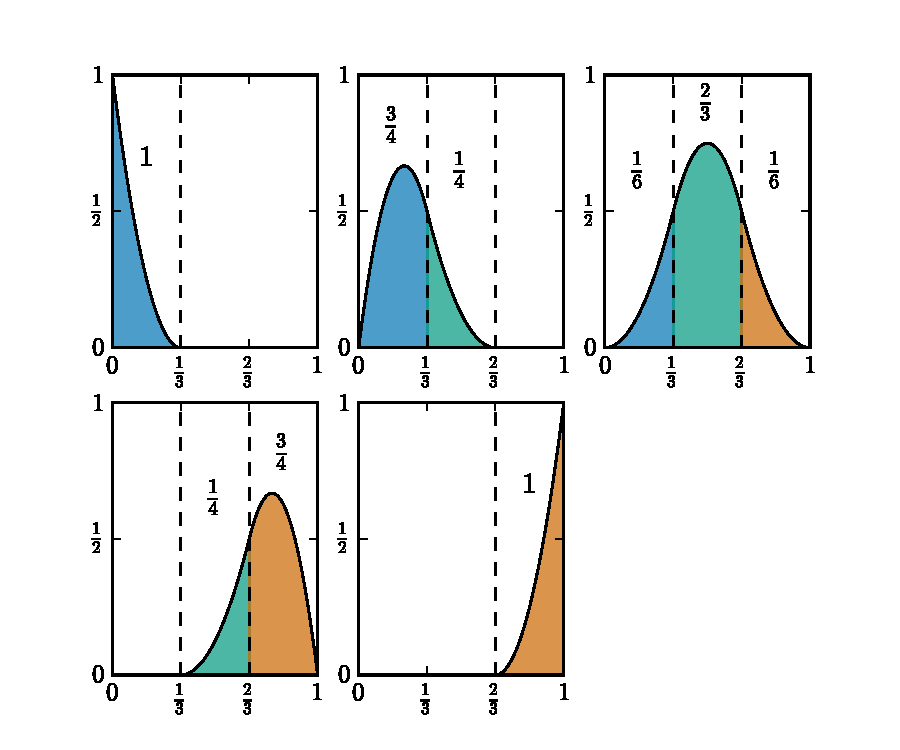
\includegraphics[width=5in]{weights.pdf}
    \caption{\label{fig:weights}Weights over each knot span associated
        with the basis function defined by the knot vector
        $[0,0,0,\frac{1}{3},\frac{2}{3},1,1,1]$.}
\end{figure}
\begin{figure}[htb]
    \centering
    \begin{tabular}{c p{4in} p{2in}}
        (0) & \raisebox{-.5\height}{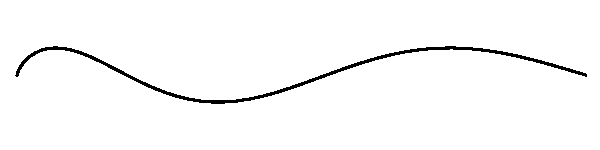
\includegraphics[width=4in]{local_proj_steps1.pdf}} & \begin{minipage}[t]{2in}Target function\end{minipage} \\
        (1) & \raisebox{-.5\height}{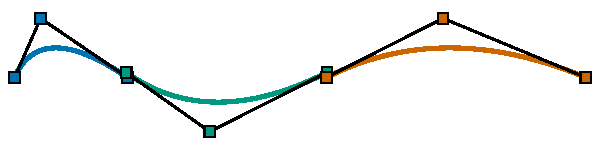
\includegraphics[width=4in]{local_proj_steps2.pdf}} & \begin{minipage}[t]{2in}Perform local projection to obtain \Bezier control points (represented by squares, colored to match elements)\end{minipage} \\
        (2) & \raisebox{-.5\height}{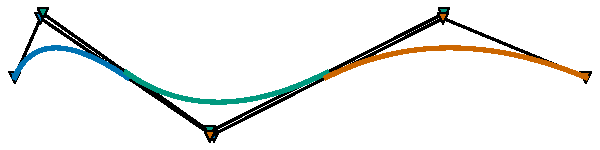
\includegraphics[width=4in]{local_proj_steps3.pdf}} & \begin{minipage}[t]{2in}Use element reconstruction operator to project \Bezier points to spline control points (represented by inverted triangles, colored to match elements)\end{minipage} \\
        (3) & \raisebox{-.5\height}{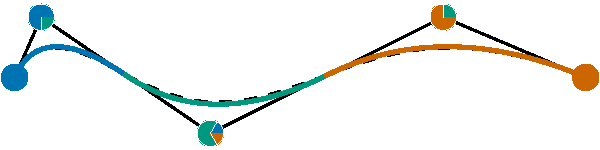
\includegraphics[width=4in]{local_proj_steps4.pdf}} & \begin{minipage}[t]{2in}Apply smoothing algorithm (contribution of each element to each control point shown by colored fraction)\end{minipage} \\
        (4) & \raisebox{-.5\height}{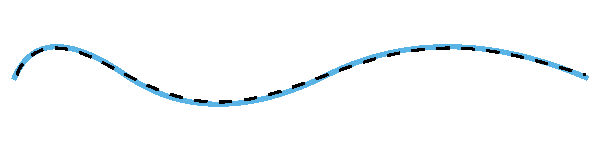
\includegraphics[width=4in]{local_proj_steps5.pdf}} & \begin{minipage}[t]{2in}Comparison of final function (light blue) and target function (dashed)\end{minipage}
    \end{tabular}
    \caption{\label{fig:loc-proj-example}Steps of \Bezier projection.}
\end{figure}

\section{Dual basis}\label{sec:dual_basis}
%%TODO: bezier dual basis function will be used for what?
In this section, we give a brief introduction to the concept of global and \Bezier dual basis functions. \Bezier dual basis functions will be used in Section to facilitate the solution of domain coupling problems in the dual mortar method. A dual basis is defined as a set of basis functions $\{\hat{N}_i\}_{i=1}^{n}$, which are dual to a corresponding set of primal basis functions $\{{N}_i\}_{i=1}^{n}$ in the sense that
\begin{equation}\label{eq:def:dual}
    \langle\hat{N}_i,N_j\rangle_\Omega:=\int_\Omega\hat{N}_iN_jd\Omega=\delta_{ij}, \quad\forall{}i,j\in\left[1,2,\dots,n\right],
\end{equation}
where $\delta_{ij}$ is the Kronecker delta.

\subsection{Global dual basis}

The global dual basis functions  $\{\hat{N}_i^G\}_{i=1}^{n}$ for a given set of primal basis function $\{{N}_i\}_{i=1}^{n}$ can be computed as
\begin{equation}
    \hat{N}_i^G=\sum_j G^{-1}_{ij}N_j,\label{eq:global_dual}
\end{equation}
where  $G^{-1}_{ij}$ are the components of the inverse of the Gramian matrix $\mathbf{G}$ with components $G_{ij}=\langle{N}_i,N_j\rangle_\Omega$.


In Isogeometric Analysis, we choose B-spline functions as the primal basis. One important property of B-spline functions is that they have compact support. This leads to sparse linear systems when these functions are used to define the trial and weighting function spaces in a Galerkin method. The global dual basis functions, however, do not have compact support and will result in dense linear systems when used as the weighting function space in a Galerkin method. Dual basis supports are shown in Figure~\ref{fig:bezier_extraction_illustration} where we have highlighted one B-spline function in Figure~\ref{fig:b-spline-func} and then shown the corresponding global dual basis function in Figure~\ref{fig:global_dual}.

\begin{figure}[ht]
    \center
    \begin{subfigure}{\linewidth}
        \center
        \includestandalone[scale=1]{basisfunctions}
        \caption{}\label{fig:b-spline-func}
    \end{subfigure}
    \begin{subfigure}{\linewidth}
        \center
        \includestandalone[scale=1]{dual_global_one}
        \caption{}\label{fig:global_dual}
    \end{subfigure}
    \begin{subfigure}{\linewidth}
        \center
        \includestandalone[scale=1]{bezier_dual_one}
        \caption{}\label{fig:bezier_dual}
    \end{subfigure}
    % or use \input{mytikz}
    \caption{A comparison of a B-spline basis function (a) with the corresponding global dual basis function (b) and the \Bezier dual basis function (c).}
    \label{fig:bezier_extraction_illustration}
\end{figure}

\subsection{\Bezier dual basis}

To maintain the sparsity of linear systems we will use \Bezier dual basis functions, which are computed locally and have compact support. These functions are computed using the \Bezier projection operator introduced in~\cite{thomas_bezier_2015}. The \Bezier dual basis has been shown to be effective in reducing volumetric and shear locking~\cite{MIAO2018273}, alleviating membrane locking in Kirchhoff-Love shells~\cite{greco2018reconstructed}, and as a dual mortaring strategy for elasticity problems~\cite{zou2018isogeometric}.

The construction of \Bezier dual basis functions leverages \Bezier extraction/projection~\cite{borden2011isogeometric, thomas2015bezier} and can be performed in several simple steps. For a given \Bezier element, $\Omega_e$, the element extraction operator $\mathbf{C}^e$ is computed. The element extraction operator maps a set of Bernstein polynomials $\{B_i\}_{i=1}^m$ defined over a \Bezier element, where $m$ depends on the polynomial degree of the \Bezier element in each parametric direction, into the set of global B-spline basis functions that have support over that element. The element reconstruction operator, $\mathbf{R}^e$, and the Gramian matrix, $\mathbf{G}^{e}$~\eqref{eq:element_gramian}, of the Bernstein polynomials defined over the element are then computed. The element extraction operator for the dual basis is then simply
\begin{equation}
    \hat{\mathbf{D}}^e=\text{diag}(\omega^e)\mathbf{R}^e\left[\mathbf{G}^{e}\right]^{-1}
\end{equation}
where $\text{diag}(\omega^e)$ is a diagonal matrix with the \Bezier projection weights~\eqref{eq:Bezier_weight} on the diagonal.

The restriction of a \Bezier dual basis functions $\hat{N}_i^B$ to $\Omega_e$ is then computed as
\begin{equation}
    \hat{N}^B_i\vert_{\Omega_e}=\sum_{j=1}^m\hat{D}^e_{ij}B_j.\label{eq:bezier-dual-basis}
\end{equation}
From this local definition of the dual basis over an element we have
\begin{equation}
    \int_{\Omega_e}\hat{N}^B_iN_jd\Omega=\omega^e_i\delta_{ij},
\end{equation}
and
\begin{equation}
    \A_e{} \int_{\Omega_e}\hat{N}^B_iN_jd\Omega=\delta_{ij},
\end{equation}
where $\A$ is the standard assembly operator \cite{Hug00} . The \Bezier dual basis of the B-spline basis function highlighted in Figure~\ref{fig:b-spline-func} is shown in Figure~\ref{fig:bezier_dual}. Note that the \Bezier dual basis function has the same compact support as the primal B-spline basis function.

\subsection{Rational dual basis functions}
If rational basis functions are used, the construction of the dual basis must be modified slightly. A rational dual basis must satisfy the biorthogonality requirement
\begin{align}
    \int_{\Omega} \bar{R}_A R_B \, d\Omega= \delta_{AB}.
\end{align}
A simple way to achieve biorthogonality is to define
\begin{align}
    \bar{R}_A & = W \bar{N}_A/w_A
\end{align}
where $W$ is the rational weight given in (\ref{eq:weight}). Now
\begin{align}
    \int_{\Omega} \bar{R}_A R_B \, d\Omega & = \int_{\Omega} \bar{N}_A N_B \, d\Omega = \delta_{AB}.
\end{align}

\begin{remark}
    The \Bezier dual basis functions define a quasi-interpolation operator $\mathcal{T}(f)=\sum_i \langle\hat{N}^B_i,f\rangle N_i$, which possesses the following properties:
    \begin{itemize}
        \item Optimal approximation: for $p^\text{th}$ order spline basis function and $f\in C^\infty$, the approximation error is given by~\cite{thomas_bezier_2015}
              \begin{equation}
                  \|\mathcal{T}(f)-f\|_{L^2}\leq Ch^{p+1}\|f\|_{H^{p+1}}.
              \end{equation}
        \item Boundary interpolation: for two sets of $p^\text{th}$ order spline basis functions $\{{N^s_i}\}_{i=1}^{n_s}$ and $\{{N^m_i}\}_{i=1}^{n_m}$ defined on $\left[{0,L}\right]$, if the first and last elements of $s$ are subsets of the first and last elements of $m$, then
              \begin{equation}
                  \mathcal{T}^s(f^m)(0)=f^m(0)\;\text{ and }\;\mathcal{T}^s(f^m)(L)=f^m(L),\quad\forall f^m\in\spn\{{N^m_i}\}_{i=1}^{n_m}.\label{eq:boundary_interpolation}
              \end{equation}
    \end{itemize}
    The second property is critical for the coercivity of the biharmonic problem on multi-patch domains.
\end{remark}
% \chapter{Isogeometric B\'ezier dual mortaring: The biharmonic problem}
\label{chp:chapter3}
\graphicspath{{figures/}{figures/chapter3/}}
\pgfplotsset{
  table/search path={{figures/chapter3/data},{data}},
}

In this dissertation, we assume that some form of reparameterization has been performed (see Figure~\ref{fig:geometries} on the right) on a CAD model to either remove some or all of the trimming curves and/or to restructure the underlying patch layout to improve the parameterization (e.g., reduce degree, distortion, complexity, etc.). However, we relax the requirement that adjacent patches share a consistent parameterization along shared edges and instead introduce a dual mortaring along the shared interfaces. Relaxing this requirement can simplify the reparameterization process leading to more robust approaches~\cite{xu2011parameterization}. This dual mortaring can be built into the simulation technology directly or can be used to build a weakly continuous basis which can then be used for either design or analysis. The present work leverages B\'ezier dual mortaring along each patch interface. In particular, in this work, the B\'ezier dual mortaring approach, introduced in~\cite{zou2018isogeometric}, is extended to biharmonic problems, which require the weak satisfaction of $C^1$ continuity. To preserve the sparsity of the condensed linear system, we propose a dual mortar suitable $C^1$ constraint and the corresponding Lagrange multiplier. Several different treatments of extraordinary points are considered. Numerical benchmarks illustrate the accuracy and robustness of the proposed method for both $2^\text{nd}$ and $4^\text{th}$ order problems.\par

\section{The dual mortar method}
\label{sec:dual-mortar-method}
We introduce the dual mortar method in the context of an abstract formulation for a constrained problem: find $u\in\mathcal{X}$ and $\lambda\in\mathcal{M}$ such that
\begin{equation}\label{eq:LM-form}
  \left\{\begin{alignedat}{2}
    a(v,u)+b(v,\lambda)&=l(v)\quad &&\forall{}v\in\mathcal{X},\\
    b(\mu,u)&=0\quad &&\forall{}\mu\in\mathcal{M},
  \end{alignedat}\right.
\end{equation}
where $a(\cdot,\cdot)$ is a bilinear form representing a potential energy, $l(\cdot)$ is a linear form representing the external load and $b(\cdot,\cdot)$ is a bilinear form representing a set of constraints on the solution $u$. In Section~\ref{sec:dual-mortar-formulation}, $b(\cdot,\cdot)$ will represent the continuity constraints across patch boundaries.

If we introduce a pair of discrete function spaces $\mathcal{X}^h \subset \mathcal{X}$ and $\mathcal{M}^h \subset \mathcal{M}$ we can represent the weak form~\eqref{eq:LM-form} as the matrix problem
\begin{equation}\label{eq:disc-LM-form}
  \mathbf{K}^\text{LM}\mathbf{U}^{\text{LM}}=\begin{bmatrix}
    \mathbf{K} & \mathbf{B}^T \\
    \mathbf{B} & \mathbf{0}
  \end{bmatrix}\mathbf{U}^{\text{LM}}
  =
  \begin{bmatrix}
    \mathbf{F} \\
    \mathbf{0}
  \end{bmatrix},
\end{equation}
where $\mathbf{K}$ is the discretized stiffness matrix, $\mathbf{F}$ is the discretized external force vector, $\mathbf{B}$ is the discretized constraints matrix and $\mathbf{U}^{\text{LM}}$ is a vector containing the control values of the displacement field $u^h \in \mathcal{X}^h$ and Lagrange multiplier field $\lambda^h \in \mathcal{M}^h$. The stiffness matrix $\mathbf{K}^\text{LM}$ for the discrete problem~\eqref{eq:disc-LM-form} always contains both positive and negative eigenvalues, for which iterative methods are known to be less efficient than for symmetric positive definite systems. More importantly, the constraint matrix $\mathbf{B}$ might be row-wise linearly dependent if the Lagrange multiplier space $\mathcal{M}^h$ is not discretized with caution. This will lead to a non-invertible linear system. The mortar method resolves these issues by introducing a constrained function space
\begin{equation}
  \mathcal{K}\coloneq\{u\in\mathcal{X}\, | \, b(\lambda,u)=0, \quad \forall{}\lambda\in\mathcal{M}\}.
\end{equation}
The saddle point problem~\eqref{eq:LM-form} can now be transformed into a minimization problem: find $u\in\mathcal{K}$ such that
\begin{equation}
  a(v, u)=l(v),\quad \forall{}v\in\mathcal{K}.
\end{equation}
Given $\mathbf{N}$, the vector containing the basis functions of $\mathcal{X}^h$, the vector containing the basis functions of $\mathcal{K}^h$ is given by
\begin{equation}
  \mathbf{N}^k=\mathbf{C}^T\mathbf{N},\label{eq:basis-null-space}
\end{equation}
where the matrix $\mathbf{C}$ is the vector basis of the null space of the constraint matrix $\mathbf{B}$. If the Lagrange multiplier space is discretized by a set of dual basis functions, the constraint matrix $\mathbf{B}$ can be written as~\cite{gilbert1987computing}
\begin{equation}\label{eq:constraint-form}
  \mathbf{B}=\begin{bmatrix}
    \mathbf{B}_1 & \mathbf{B_2}
  \end{bmatrix},
\end{equation}
where $\mathbf{B}_1$ is an identity matrix, and the bandwidth of $\mathbf{B}_2$ depends on the support size of dual basis functions. For a constraint matrix $\mathbf{B}$ constructed using \Bezier dual basis functions, $\mathbf{B}_2$ is a sparse matrix with limited bandwidth, while the global dual basis functions leads to a dense $\mathbf{B}_2$.\par

For a $\mathbf{B}$ in the form~\eqref{eq:constraint-form} with $\mathbf{B}_1 = \mathbf{I}$, the vector basis of its null space can be obtained from
\begin{equation}
  \mathbf{C}=\begin{bmatrix}
    -\mathbf{B}_2 \\
    \mathbf{I}
  \end{bmatrix}.
  \label{eq:null-space}
\end{equation}
The mortar linear system can now be written as
\begin{equation}
  \mathbf{K}^{\text{mortar}}\mathbf{U}^{\text{mortar}}=\mathbf{C}^T\mathbf{K}\mathbf{C}\mathbf{U}^{\text{mortar}}=\mathbf{C}^T\mathbf{F}.\label{eq:mortar-form-discretized}
\end{equation}
The relation between the mortar displacement nodal value vector $\mathbf{U}^{\text{mortar}}$ and $\mathbf{U}^{\text{LM}}$ is given by
\begin{equation}
  \mathbf{U}^{\text{LM}}=\mathbf{C}\mathbf{U}^{\text{mortar}}.
\end{equation}
With a sparse $\mathbf{C}$ obtained from the \Bezier dual basis, the stiffness matrix of the mortar formulation $\mathbf{K}^{\text{mortar}}$ will remain sparse, resulting in an efficient linear system.

\section{A dual mortar formulation for the multi-patch biharmonic problem}
\label{sec:dual-mortar-formulation}

In this section, we present a formulation for the biharmonic problem over multi-patch tensor product domains. Because the biharmonic problem requires trial and test functions that are in $H^2$, we will use the dual mortar method to add constraints between patch boundaries to weakly enforce $C^1$ continuity. We begin by introducing concepts from domain decomposition.

\subsection{Domain decomposition}\label{sec:domain_decompostion}

Let $\Omega$ be a bounded open domain in $\mathbb{R}^2$ with its boundary denoted by $\partial\Omega$. We assume that $\Omega$ can be subdivided into $K$ non-overlapping patches $\Omega_k$ for $1\leq{}k\leq{}K$, i.e.
\begin{equation}
  \bar{\Omega} = \bigcup_{k=1}^{K} \bar{\Omega}_{k}  \quad \textrm{and} \quad {\Omega}_{k}\bigcap{\Omega}_{l}=\emptyset, \quad \forall k\neq{l}
\end{equation}
where $\bar{\Omega}_k$ is the closure of $\Omega_k$. For simplicity, we only consider the case where the intersection of two patches is either empty, a single vertex, or the entire edge. We denote the common interface of two neighboring patches as $\Gamma_{kl} = \partial{\Omega}_k\bigcap\partial{\Omega}_l$ so that $\Gamma_{kl}=\emptyset$ if $\Omega_k$ is not a neighbor of $\Omega_l$. We also define the skeleton $\mathbf{S}=\bigcup_{k,l\in{K}, k<{l}}\Gamma_{kl}$ as the union of all interfaces in $\Omega$. The set $\mathbf{V}$ denotes the set of all vertices in $\Omega$. A representative example of a multi-patch geometry is shown in Figure~\ref{fig:partition}.

\begin{figure}[ht]
  \center
  \includestandalone[scale=1]{patch_partition}
  % or use \input{mytikz}
  \caption{An example of a domain decomposition of a triangular domain. The patches are defined on different parametric domains and are connected via geometric mappings.}
  \label{fig:partition}
\end{figure}

For each patch, there exists a bijective geometric mapping from the parametric domain $\hat{\Omega}_k$ to the physical domain $\Omega_k$, which is defined as
\begin{equation}
  \mathbf{F}_{k}\left(\xi_{k},\eta_{k}\right)\colon{\hat{\Omega}_k}\mapsto{{\Omega}_k}\in\mathbb{R}^2,
\end{equation}
where $\left(\xi_{k},\eta_{k}\right)$ are the coordinates of the parametric domain. For simplicity and without loss of generality, we assume the parametric domain is ${\hat{\Omega}_k}=\left[{0,1}\right]\times\left[{0,1}\right]$ for all patches.

We can use the mappings $\mathbf{F}_k$ to create connections between neighboring patches. Due to the fact that $\mathbf{F}_k$ is a bijection, there exists an inverse mapping denoted by $\mathbf{F}^{-1}_k$. We can construct a bijective transformation on the intersection $\Gamma_{kl}$ as
\begin{equation}
  \mathbf{E}_{kl}=\mathbf{F}_{l}^{-1}\circ\mathbf{F}_{k},
\end{equation}
which maps a parametric point on $\partial{\hat{\Omega}}_k\bigcap \hat{\Gamma}_{kl}$ to a physical point on the intersection $\Gamma_{kl}$ and then to a parametric point on $\partial{\hat{\Omega}}_l\bigcap \hat{\Gamma}_{kl}$. With the mapping $\mathbf{E}_{kl}$ in hand, we are now ready to formulate the biharmonic problem over multi-patch domains.

\subsection{The biharmonic problem}

The strong form governing equation and boundary conditions of the homogeneous biharmonic problem defined over the domain $\Omega$ is given by the following:

\begin{equation}\label{eq:strong-form}
  \left\{\begin{alignedat}{2}
    \Delta^2u&=f\quad &&\text{on }\Omega,\\
    u=\frac{\partial{u}}{\partial{\mathbf{n}}}&=0\quad &&\text{on }\partial\Omega,
  \end{alignedat}\right.
\end{equation}
with $f\in{}L^2(\Omega)$ and $u\in{}C^4(\Omega)$. This problem can be restated in the weak form as: find $u\in{}H^2_0(\Omega)$ such that
\begin{equation}\label{eq:weak-form}
  a_b(u,v)=l(v),\quad\forall{}v\in{}H^2_0(\Omega),
\end{equation}
with
\begin{equation}
  \begin{split}
    a_b(u,v)&=\int_{\Omega}\nabla u \nabla v d \Omega,\\
    l(v) &= \int_{\Omega} fv d \Omega,
  \end{split}
\end{equation}
where $H^2_0(\Omega)$ is the Sobolev space containing all functions in the space $H^2(\Omega)$ that also satisfy the homogeneous Dirichlet boundary conditions in~\eqref{eq:strong-form}.

For a partitioned domain $\Omega$, as defined in Section~\ref{sec:domain_decompostion}, the construction of a finite dimensional subspace of $H^2_0(\Omega)$ is a nontrivial task because there is no guarantee that the discretization of neighboring domains is smooth enough across shared boundaries to satisfy the $H^2(\Omega)$ requirement. In order to handle multi-patch geometries, we will recast the biharmonic problem in terms of the following Lagrange multiplier formulation: find $u\in{\mathcal{X}_b}$, $\lambda_0\in{\mathcal{M}_0}$ and $\lambda_1\in{\mathcal{M}_1}$ such that:
\begin{equation}
  \left\{\begin{alignedat}{2}
    a_b(u,v)+b_0(\lambda_0,v)+b_1(\lambda_1,v)&=l(v)\quad&&\forall v\in{\mathcal{X}_b},\\
    b_0(\mu_0,u)&=0 \quad&&\forall \mu_0\in{\mathcal{M}_0},\\
    b_1(\mu_1,u)&=0 \quad&&\forall \mu_1\in{\mathcal{M}_1},
  \end{alignedat}\right.
\end{equation}
where
\begin{equation}
  \mathcal{X}_b\coloneq\{v\in{}L^2(\Omega)\,\vert\,{}v\vert_{\Omega_k}\in{}H^2(\Omega_k),\,{}1\leq{}k\leq{}K\text{  and }v\vert_{\partial{}\Omega}=\frac{\partial{}v}{\partial{\mathbf{n}}}\vert_{\partial{}\Omega}=0\},
\end{equation}
is an unconstrained broken Sobolev space endowed with the norm $\|u\|_{H^2_*(\Omega)}=\left(\sum_{k=1}^K \|u\|_{H^2(\Omega_k)}\right)^{1/2}$, $\mathcal{M}_0$ and $\mathcal{M}_1$ are Lagrange multiplier spaces, and $b_0$ and $b_1$ impose the required constraints on $u$ to satisfy the $H^2$ requirement. We will define $b_0$ and $b_1$ in the following section.

\begin{remark}
  Strictly speaking, the restriction of $u\in{}H^2(\Omega)$ to the boundary $\partial\Omega$ is ill-defined. To rigorously define the value of $u$ and its normal derivative on $\partial\Omega$, we need the help of the trace operator $T$. A standard trace theorem states~\cite{grisvard2011elliptic}: Given $\Omega$ with a boundary $\partial \Omega$ of class $C^{k,1}$ (i.e., $k$ times continuously differentiable and its $k^\text{th}$ order derivatives are Lipschitz continuous). Assume that $l\leq k$. Then the mapping
  \begin{equation}
    u \rightarrow \{Tu, T\frac{\partial u}{\partial \mathbf{n}}, \dots, T\frac{\partial^l u}{\partial^l \mathbf{n}}\},
  \end{equation}
  is a bounded linear operator from $H^{k+1}(\Omega)$ onto $\prod_{j=0}^lH^{k-j+\frac{1}{2}}(\partial \Omega)$. And if $u\in{}H^{k+1}(\Omega)\cap{}C^\infty(\Omega)$, we have the following relation
  \begin{equation}
    \{u, \frac{\partial u}{\partial \mathbf{n}}, \dots, \frac{\partial^l u}{\partial^l \mathbf{n}}\} =
    \{Tu, T\frac{\partial u}{\partial \mathbf{n}}, \dots, T\frac{\partial^l u}{\partial^l \mathbf{n}}\}
  \end{equation}
  Hence, for $u\in{}H^2(\Omega)$, we have $Tu\in H^{\frac{3}{2}}(\partial \Omega)$ and $T\frac{\partial u}{\partial \mathbf{n}}\in H^{\frac{1}{2}}(\partial \Omega)$. If $u\circ \mathbf{F} \in H^2({\hat{\Omega}})$ and each entries of $\nabla \mathbf{F}^{-1}$ are in $L^{\infty}(\Omega)$, then~\cite{ciarlet1972interpolation}
  \begin{equation}
    \begin{bmatrix}
      \frac{\partial u\circ \mathbf{F}}{\partial \xi} \circ \mathbf{F}^{-1} \\
      \frac{\partial u\circ \mathbf{F}}{\partial \eta} \circ \mathbf{F}^{-1}
    \end{bmatrix}
    \in H^{1}(\Omega)^2.
  \end{equation}
  As a result, $T\left(\frac{\partial u\circ \mathbf{F}}{\partial \xi} \circ \mathbf{F}^{-1}\right)\in H^{\frac{1}{2}}(\partial \Omega)$ and $T\left(\frac{\partial u\circ \mathbf{F}}{\partial \eta} \circ \mathbf{F}^{-1}\right)\in H^{\frac{1}{2}}(\partial \Omega)$.\par
  This result guarantees $H^2_0(\Omega)$ and the inter-patch constraints that will be discussed in the next section are all well-defined. In order to avoid cumbersome notation, the trace operator $T(\cdot)$ is suppressed and we will use $\{ \frac{\partial u}{\partial \xi}, \frac{\partial u}{\partial \eta} \}$ to refer to $\{ \frac{\partial u\circ \mathbf{F}}{\partial \xi} \circ \mathbf{F}^{-1},\frac{\partial u\circ \mathbf{F}}{\partial \eta} \circ \mathbf{F}^{-1} \}$.
\end{remark}

\subsection{Dual-compatible $C^1$ constraints}

We now develop a set of constraints to impose $C^1$ continuity across patch boundaries under the dual mortar framework. Since $C^1(\Omega) \subset H^2(\Omega)$, we will be able to use these constraints to solve the multi-patch biharmonic problem.\par

To illustrate our method, we consider the construction of $C^1$ constraints for the two-patch domain shown in Figure~\ref{fig:two-patch-mesh}. We call $\Omega_s$ the slave domain and $\Omega_m$ the master domain. For a function $u \in C^1( \Omega_s \cup \Omega_m )$ with
\begin{equation}
  u=
  \begin{cases}
    u_s\quad \text{in }\Omega_s \\
    u_m\quad \text{in }\Omega_m,
  \end{cases}
\end{equation}
and $u_s\in{}C^1(\Omega_s)$, $u_m\in{}C^1(\Omega_m)$ the following two constraints are required across the intersection $\Gamma_{sm}$:
\begin{subequations}
  \begin{align}
    [u]_{\Gamma_{sm}}                                                   & =0,\label{eq:biharmonic_c0}                                                        \\
    \left[\frac{\partial{u}}{\partial{\mathbf{n}}}\right]_{\Gamma_{sm}} & =0,\quad\text{with }\mathbf{n}=\mathbf{n}_s=-\mathbf{n}_m,\label{eq:biharmonic_c1}
  \end{align}
\end{subequations}
where $\mathbf{n}_k$ is the outward normal direction of $\partial{\Omega_k}$ and
\begin{equation}
  [\cdot]_{\Gamma_{sm}}\coloneq\cdot\vert_{\Omega_s}-\cdot\vert_{\Omega_m}
  %   \scott{Check this notation, it doesn't see quite right}
\end{equation}
is the jump operator. The continuity constraint~\eqref{eq:biharmonic_c0} can naturally be incorporated into the framework of the dual mortar formulation. The smoothness constraint~\eqref{eq:biharmonic_c1}, however, can not be directly imposed. First, the existence of a dual basis for $\frac{\partial{N_i}}{\partial{\mathbf{n}}}\vert_{\Gamma_{sm}}$ is doubtful. Even if these dual basis functions do exist, since they are biorthogonal to the normal derivative of the basis functions, their formulation will depend on the parameterization of $\Gamma_{sm}$ and the geometric information of $\Omega_s$. This complex geometric dependence would destroy the simplicity of the dual basis formulation. To overcome this issue, we instead propose a smoothness constraint involving parametric derivatives only.
\begin{figure}[ht]
  \center
  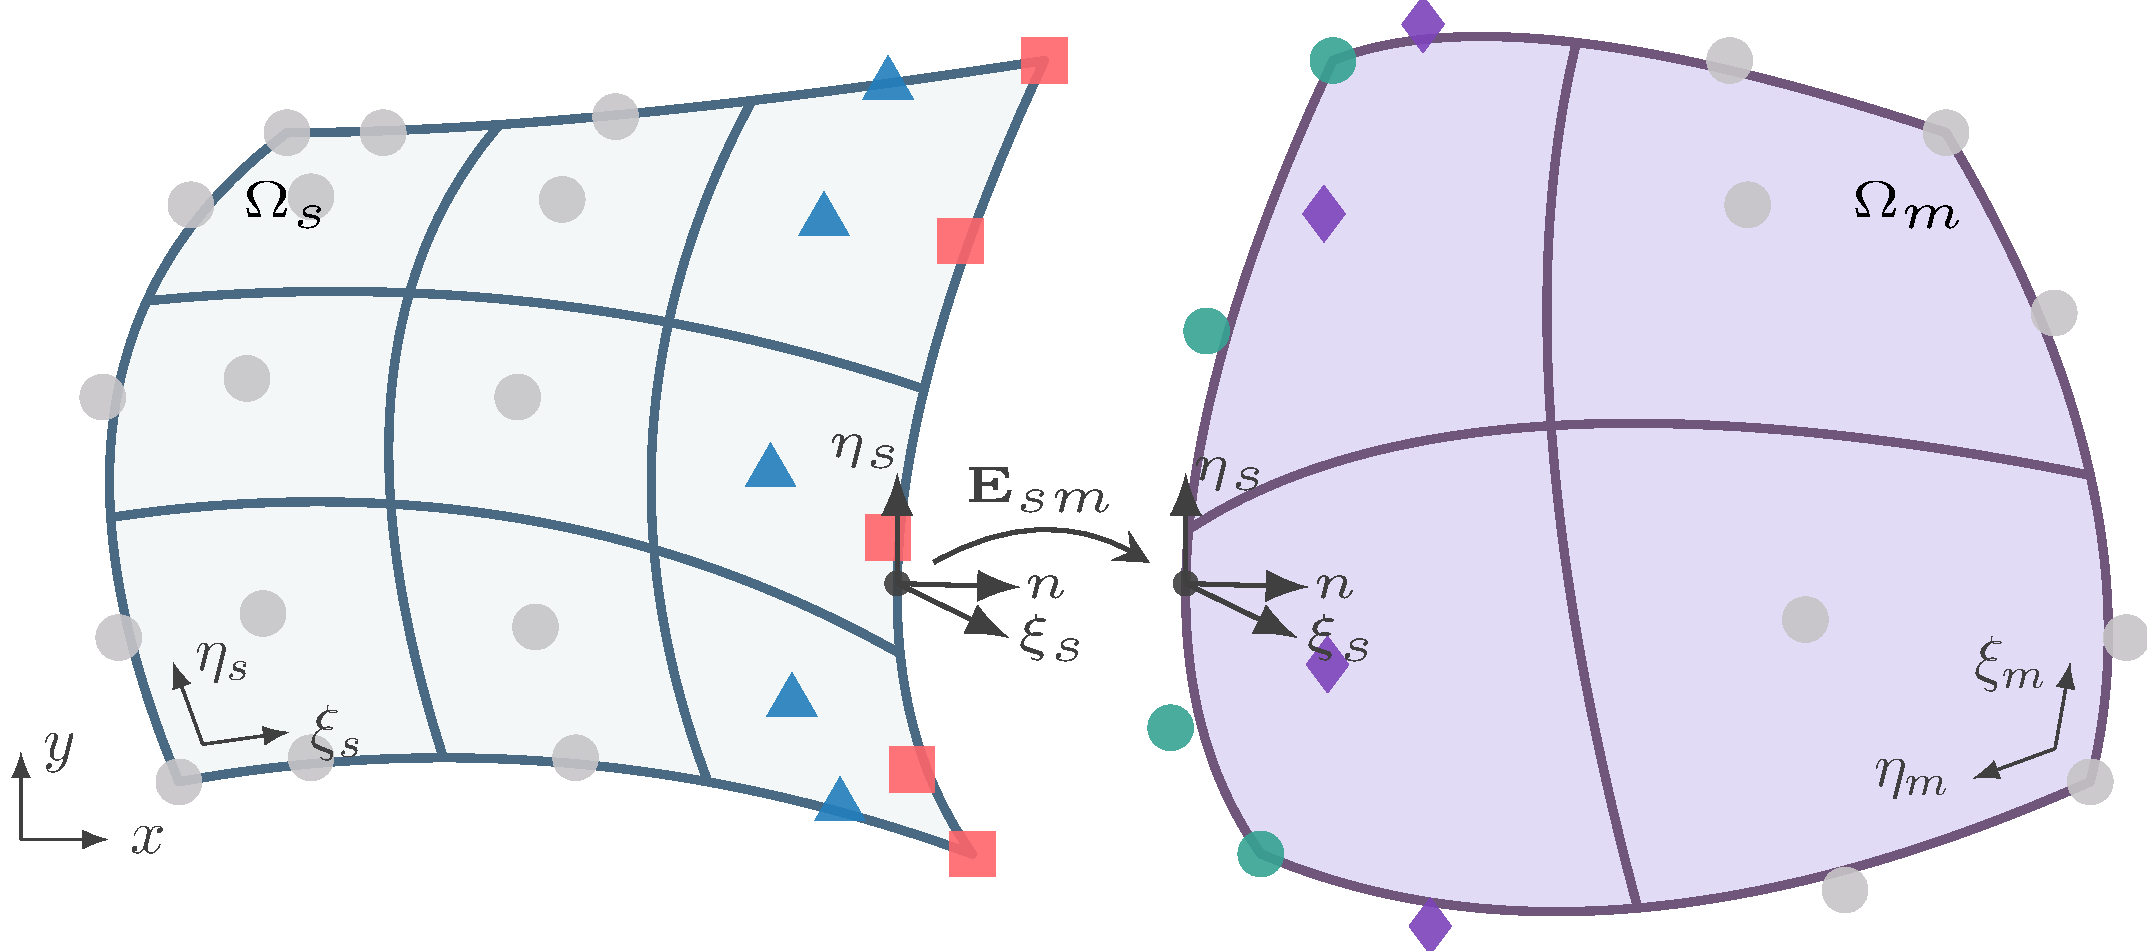
\includegraphics[scale=.4]{two-patch-mesh}
  % or use \input{mytikz}
  \caption{A two-patch planar domain $\Omega$ consisting of two patches $\Omega_s$ and $\Omega_m$ that are defined by the two mappings $\mathbf{F}_s$ and $\mathbf{F}_m$.}
  \label{fig:two-patch-mesh}
\end{figure}

\begin{lemma}
  Given two differentiable bijective geometric mappings $\mathbf{F}_{s}\colon\hat{\Omega}_s\rightarrow{\Omega}_s$ and $\mathbf{F}_{m}\colon\hat{\Omega}_m\rightarrow{\Omega}_m$, a $C^0$-continuous function $u$ is $C^1$-continuous in the physical domain if and only if
  \begin{equation}
    \left[\frac{\partial{u}}{\partial{\mathbf{\xi}_s}}\right]_{\Gamma_{sm}}=0\quad\text{ and }\quad\left[\frac{\partial{u}}{\partial{\mathbf{\eta}_s}}\right]_{\Gamma_{sm}}=0. \label{eq:biharmonic_c1_mod}
  \end{equation}

  \begin{proof}
    It suffices to consider two neighboring patches as shown in Figure~\ref{fig:two-patch-mesh}. In this configuration, if $u$ is a $ C^0$-continuous function then $[\frac{\partial{u}}{\partial{\mathbf{\eta}_s}}]_{\Gamma_{sm}}=0$. If $u$ is also $C^1$-continuous, we have
    \begin{equation}
      0=\left[\frac{\partial{u}}{\partial{\mathbf{n}}}\right]_{\Gamma_{sm}}=\left[\frac{\partial{u}}{\partial{\mathbf{\xi}_s}}\right]_{\Gamma_{sm}}\frac{\partial{}\xi_s}{\partial{\mathbf{n}}}+\left[\frac{\partial{u}}{\partial{\mathbf{\eta}_s}}\right]_{\Gamma_{sm}}\frac{\partial{}\eta_s}{\partial{\mathbf{n}}}\Longrightarrow\left[\frac{\partial{u}}{\partial{\mathbf{\xi}_s}}\right]_{\Gamma_{sm}}\frac{\partial{}\xi_s}{\partial{\mathbf{n}}}=0
    \end{equation}
    The fact that $\mathbf{F}_{s}$ is bijective and $\frac{\partial{}\eta_s}{\partial{\mathbf{n}}} = 0$ indicates $\frac{\partial{}\xi_s}{\partial{\mathbf{n}}}\neq{}0$. Hence, $\left[\frac{\partial{u}}{\partial{\mathbf{\xi}_s}}\right]_{\Gamma_{sm}}=0$. On the other hand,
    \begin{equation}
      \begin{cases}
        \left[\frac{\partial{u}}{\partial{\mathbf{\xi}_s}}\right]_{\Gamma_{sm}}=0 \\
        \left[\frac{\partial{u}}{\partial{\mathbf{\eta}_s}}\right]_{\Gamma_{sm}}=0
      \end{cases}
      \Longrightarrow
      \left[\frac{\partial{u}}{\partial{\mathbf{n}}}\right]_{\Gamma_{sm}}=\left[\frac{\partial{u}}{\partial{\mathbf{\xi}_s}}\right]_{\Gamma_{sm}}\frac{\partial{}\xi_s}{\partial{\mathbf{n}}}+\left[\frac{\partial{u}}{\partial{\mathbf{\eta}_s}}\right]_{\Gamma_{sm}}\frac{\partial{}\eta_s}{\partial{\mathbf{n}}}=0
    \end{equation}
    This concludes the proof.
  \end{proof}
\end{lemma}

Hence, the constraints in~\eqref{eq:biharmonic_c1_mod} are equivalent to constraint~\eqref{eq:biharmonic_c1}. On an intersection that is parallel to the $\eta_s$ direction in the parametric domain, the constraint $\left[\frac{\partial{u}}{\partial{\mathbf{\xi}_s}}\right]_{\Gamma_{sm}}=0$ is utilized; on an intersection that is parallel to the $\xi_s$ direction in the parametric domain, the constraint $\left[\frac{\partial{u}}{\partial{\mathbf{\eta}_s}}\right]_{\Gamma_{sm}}=0$ is utilized.

\begin{remark}
  In order to demonstrate the advantages of the constraints in~\eqref{eq:biharmonic_c1_mod}, we consider the following intergral:
  %   \scott{what is the -1 in the integral mean?}
  \begin{equation}
    \begin{split}
      \int_{\Gamma_{sm}}\frac{\partial{}N_a(\xi_s,\eta_s)}{\partial{}\xi_s}\hat{N}_{j}(\eta_s)d\Gamma&=\int_{\Gamma_{sm}}\frac{\partial{}N_{n_{\xi_s}-1}(1)N_{i}(\eta_s)}{\partial{}\xi_s}\hat{N}_{j}(\eta_s)d\Gamma\\
      &=\frac{\partial{}N_{n_{\xi_s}-1}(1)}{\partial{}\xi_s}\int_{\Gamma_{sm}}N_{i}(\eta_s)\hat{N}_{j}(\eta_s)d\Gamma
    \end{split}\quad i,j\in\left\{1,2,\dots, n_{\eta_s}\right\}
    \label{eq:advan_constraint}
  \end{equation}
  where $n_{\xi_s}$ and $n_{\eta_s}$ are the number of nodes in the $\xi_s$ and $\eta_s$ directions of the slave patch, respectively, and the index $a = n_{\xi_s}i-1$. This integral is one term that is involved in the discretization of the constraint~\eqref{eq:biharmonic_c1} and is constructed by a Lagrange multiplier basis function $\hat{N}_j(\eta_s)$ and an activated basis function of the slave patch $N_a(\xi_s,\eta_s)$ that is one column away from the intersection (denoted by the blue triangles in Figure~\ref{fig:two-patch-mesh}). Due to the tensor product structure of multivariate spline basis functions, the derivative in one direction ($\xi_s$ for this case) will not influence the contributions coming from other directions. Hence, the dual basis function of an activated basis function in the constraint $\left[\frac{\partial{u}}{\partial{\mathbf{\xi}_s}}\right]_{\Gamma_{sm}}=0$ can be constructed by the dual basis function of its $\eta_s$ component divided by $\frac{\partial{}N_{n_{\xi_s}-1}(1)}{\partial{}\xi_s}$.
\end{remark}
The only issue now is how to evaluate the derivative of $u_m$ w.r.t. $\xi_s$ or $\eta_s$ directions. This can be done by considering the following chain rule
\begin{align}
  \begin{bmatrix}
    \tfrac{\partial{u_m}}{\partial{\xi_s}} \\
    \tfrac{\partial{u_m}}{\partial{\eta_s}}
  \end{bmatrix}
  =
  \begin{bmatrix}
    \frac{\partial\xi_m}{\partial\xi_s}  & \frac{\partial\xi_m}{\partial\eta_s}  \\
    \frac{\partial\eta_m}{\partial\xi_s} & \frac{\partial\eta_m}{\partial\eta_s}
  \end{bmatrix}^T
  \cdot
  \begin{bmatrix}
    \tfrac{\partial{u_m}}{\partial{\xi_m}} \\
    \tfrac{\partial{u_m}}{\partial{\eta_m}}
  \end{bmatrix}
  =
  \nabla\mathbf{E}_{sm}^T
  \cdot
  \begin{bmatrix}
    \tfrac{\partial{u_m}}{\partial{\xi_m}} \\
    \tfrac{\partial{u_m}}{\partial{\eta_m}}
  \end{bmatrix}.
\end{align}
The Jacobian of the composition mapping $\mathbf{E}_{sm}$ can be written as
\begin{equation}
  \nabla\mathbf{E}_{sm}=\nabla(\mathbf{F}_{m}^{-1}\circ\mathbf{F}_{s})=\nabla(\mathbf{F}_{m}^{-1})\cdot{}\nabla\mathbf{F}_{s}=(\nabla\mathbf{F}_{m})^{-1}\cdot{}\nabla\mathbf{F}_{s}.
\end{equation}

\subsection{The dual mortar formulation}
The Lagrange multiplier formulation for the multi-patch biharmonic problem can be defined as: find $u\in{\mathcal{X}_b}$, $\lambda_0\in{\mathcal{M}_0}$ and $\lambda_1\in{\mathcal{M}_1}$ such that
\begin{equation}
  \left\{\begin{alignedat}{2}
    a_b(u,v)+b_0(\lambda_0,v)+b_1(\lambda_1,v)&=l(v)\quad&&\forall v\in{\mathcal{X}_b},\\
    b_0(\mu_0,u)&=0 \quad&&\forall \mu_0\in{\mathcal{M}_0},\\
    b_1(\mu_1,u)&=0 \quad&&\forall \mu_1\in{\mathcal{M}_1},
  \end{alignedat}\right.\label{eq:biharmonic_mixed}
\end{equation}
with
\begin{subequations}
  \begin{align}
    b_0(\lambda_0,v) & =\sum_{\Gamma\in\mathbf{S}}\int_\Gamma[u]_{\Gamma}\lambda_0d\Gamma,\label{eq:operator-b0}                                                                                                                                                                                                                          \\
    b_1(\lambda_1,v) & =\sum_{\Gamma\in\mathbf{S}}\left(\int_\Gamma\left[\frac{\partial{u}}{\partial{\xi_s}}\right]_{\Gamma}\lambda_1d\Gamma\text{ if }\Gamma\parallel\eta_s\text{ or }\int_\Gamma\left[\frac{\partial{u}}{\partial{\eta_s}}\right]_{\Gamma}\lambda_1d\Gamma\text{ if }\Gamma\parallel\xi_s\right).\label{eq:operator-b1}
  \end{align}
\end{subequations}
The constrained function space required by the dual mortar formulation of the multi-patch biharmonic problem can then be defined as
\begin{equation}
  \mathcal{K}_b:=\left\{u\in{}\mathcal{X}_b\,\vert\,b_0(\mu_0,u)=0 \text{ and }b_1(\mu_1,u)=0\,\forall(\mu_0,\mu_1)\in{\mathcal{M}_0\times{}\mathcal{M}_1}\right\}.\label{eq:constrained_space}
\end{equation}

\subsection{Discretization}

For each intersection, the two adjacent patches are classified as either slave $\Omega_s$ or master $\Omega_m$. One patch can, at the same time, be a master for one intersection and a slave for another intersection. To approximate the solution of the variational problem, we use B-spline basis functions $\{N^s_i\}_{i\in{I_s}}$ and $\{N^m_i\}_{i\in{I_m}}$ to discretize $\Omega_s$ and $\Omega_m$, respectively. Note that, on the intersection, we select the side with finer trace mesh as the slave patch and denote the other side as the master patch. This selection strategy can minimize the error from variational crimes~\cite{strang1973analysis,brenner_mathematical_2007}.
% (\scott{is this absolutely necessary? what happens if its not the case?}. 
An appropriate indexing is chosen so that there is no overlap between the index sets $I_s$ and $I_m$ (i.e., given $n_s$ basis functions in $\Omega_s$, we can assume the starting index in the index set $I_m$ is $n_s+1$). The discretized geometrical mappings are represented by
\begin{align}
  \mathbf{F}_s & =\sum_{i\in{I_s}}\mathbf{P}_i^sN_i^s, \\
  \mathbf{F}_m & =\sum_{i\in{I_m}}\mathbf{P}_i^mN_i^m,
\end{align}
where the control points $\mathbf{P}_i^s,\mathbf{P}_i^m\in\mathbb{R}^2$. The discrete space $\mathcal{X}_b^h \subset \mathcal{X}_b$ contains the discretized test and weighting functions. In other words,
\begin{equation}
  u^h=\sum_{i\in{I_s\cup{}I_m}}U_iN_i,\quad v^h=\sum_{i\in{I_s\cup{}I_m}}V_iN_i
\end{equation}
with
\begin{align}
  N_i=
  \begin{cases}
    N_i^s \quad & i\in{I_s}, \\
    N_i^m \quad & i\in{I_m}.
  \end{cases}
\end{align}
The discrete Lagrange multiplier spaces $\mathcal{M}_0^h \subset \mathcal{M}_0$ and $\mathcal{M}_1^h \subset \mathcal{M}_1^h$ are created using the dual basis. Depending on the orientation of the intersection, we have that
\begin{itemize}
  \item for the intersection $\xi_s=0$,
        \begin{equation}
          \begin{split}
            \lambda_0^h&=\sum_{i=1}^{n_{\eta_s}}\Lambda^0_i\hat{N}^s_i(\eta_s),\quad  \mu_0^h=\sum_{i=1}^{n_{\eta_s}}\delta\Lambda^0_i\hat{N}^s_i(\eta_s)\\
            \lambda_1^h&=\sum_{i=1}^{n_{\eta_s}}\Lambda^1_i\frac{\hat{N}^s_i(\eta_s)}{c}, \quad \mu_1^h=\sum_{i=1}^{n_{\eta_s}}\delta\Lambda^1_i\frac{\hat{N}^s_i(\eta_s)}{c},\quad c=\left.\frac{\partial{N^s_2(\xi_s)}}{\partial{\xi_s}}\right|_{\xi_s=0},
          \end{split}
        \end{equation}
  \item for the intersection $\xi_s=1$,
        \begin{equation}
          \begin{split}
            \lambda_0^h&=\sum_{i=1}^{n_{\eta_s}}\Lambda^0_i\hat{N}^s_i(\eta_s),\quad \mu_0^h=\sum_{i=1}^{n_{\eta_s}}\delta\Lambda^0_i\hat{N}^s_i(\eta_s)\\
            \lambda_1^h&=\sum_{i=1}^{n_{\eta_s}}\Lambda^1_i\frac{\hat{N}^s_i(\eta_s)}{c},\quad \mu_1^h=\sum_{i=1}^{n_{\eta_s}}\delta\Lambda^1_i\frac{\hat{N}^s_i(\eta_s)}{c},\quad c=\left.\frac{\partial{N^s_{n_{\xi_s}-1}(\xi_s)}}{\partial{\xi_s}}\right|_{\xi_s=1},
          \end{split}
        \end{equation}
  \item for the intersection $\eta_s=0$,
        \begin{equation}
          \begin{split}
            \lambda_0^h&=\sum_{i=1}^{n_{\xi_s}}\Lambda^0_i\hat{N}^s_i(\xi_s),\quad \mu_0^h=\sum_{i=1}^{n_{\xi_s}}\delta\Lambda^0_i\hat{N}^s_i(\xi_s)\\
            \lambda_1^h&=\sum_{i=1}^{n_{\xi_s}}\Lambda^1_i\frac{\hat{N}^s_i(\xi_s)}{c},\quad \mu_1^h=\sum_{i=1}^{n_{\xi_s}}\delta\Lambda^1_i\frac{\hat{N}^s_i(\xi_s)}{c},\quad c=\left.\frac{\partial{N^s_2(\eta_s)}}{\partial{\eta_s}}\right|_{\eta_s=0},
          \end{split}
        \end{equation}
  \item for the intersection $\eta_s=1$,
        \begin{equation}
          \begin{split}
            \lambda_0^h&=\sum_{i=1}^{n_{\xi_s}}\Lambda^0_i\hat{N}^s_i(\xi_s), \quad  \mu_0^h=\sum_{i=1}^{n_{\xi_s}}\delta\Lambda^0_i\hat{N}^s_i(\xi_s)\\
            \lambda_1^h&=\sum_{i=1}^{n_{\xi_s}}\Lambda^1_i\frac{\hat{N}^s_i(\xi_s)}{c},\quad \mu_1^h=\sum_{i=1}^{n_{\xi_s}}\delta\Lambda^1_i\frac{\hat{N}^s_i(\xi_s)}{c},\quad c=\left.\frac{\partial{N^s_{n_{\eta_s}-1}(\eta_s)}}{\partial{\eta_s}}\right|_{\eta_s=1}.
          \end{split}
        \end{equation}
\end{itemize}\par

By substituting the discretized displacement field and Lagrange multipliers into the bilinear form $a_b(\cdot,\cdot)$, $b_0(\cdot,\cdot)$ and $b_1(\cdot,\cdot)$, we obtain the following stiffness and constraint matrices
\begin{equation}
  \mathbf{V}^T\mathbf{K}_b\mathbf{U}=a_b(u^h,v^h)\quad\text{and}\quad
  \begin{bmatrix}
    \delta\mathbf{\Lambda}^0 \\
    \delta\mathbf{\Lambda}^1
  \end{bmatrix}^T\mathbf{B}_b\mathbf{U}=\begin{bmatrix}
    b_0(\mu_0^h,u^h) \\
    b_1(\mu_1^h,u^h)
  \end{bmatrix}.
\end{equation}
The remaining question is how to effectively construct the vector basis (in matrix form $\mathbf{C}_b$) of the null space of $\mathbf{B}_b$ such that the resulting basis functions (constructed by Equation~\eqref{eq:basis-null-space}) of $\mathcal{K}_b^h \subset \mathcal{K}_b$ have compact support and lead to a sparse stiffness matrix in~\eqref{eq:mortar-form-discretized}.

\section{Building a basis for the null space of $\mathbf{B}_b$}

\subsection{The two-patch case}

Recall from Section~\ref{sec:dual-mortar-method} that for a constraint matrix taking the form~\eqref{eq:constraint-form} the corresponding operator $\mathbf{C}$ can be constructed in an elegant manner via Equation~\eqref{eq:null-space}. In this section, we will show how to recover form~\eqref{eq:constraint-form} from the constraint matrix $\mathbf{B}_b$ via a simple linear transformation. We first classify the basis functions of $\mathcal{X}_b^h$ into five different types, depending on their proximity to an interface, as shown in Figure~\ref{fig:two-patch-mesh}:
\begin{enumerate}
  \item The basis functions $N^s_i$ such that $\supp{N^s_i}\bigcap\Gamma_{sm}=\emptyset$ and $\supp{\frac{\partial{}N^s_i}{\partial{\xi_s}}}\bigcap\Gamma_{sm}\neq\emptyset$ (the second closest column of slave basis functions to the intersection $\Gamma_{sm}$), whose indices are denoted by the index set $I_\text{i}$. (denoted by blue triangles)
  \item The basis functions $N^s_i$ such that $\supp{N^s_i}\bigcap\Gamma_{sm}\neq\emptyset$ (the column of slave basis functions on the intersection $\Gamma_{sm}$), whose indices are denoted by the index set $I_\text{ii}$. (denoted by red squares)
  \item The basis functions $N^m_i$ such that $\supp{N^m_i}\bigcap\Gamma_{sm}\neq\emptyset$  (the column of master basis functions on the intersection $\Gamma_{sm}$), whose indices are denoted by the index set $I_\text{iii}$. (denoted by green circles)
  \item The basis functions $N^m_i$ such that $\supp{N^m_i}\bigcap\Gamma_{sm}=\emptyset$ and $\supp{\frac{\partial{}N^m_i}{\partial{\xi_s}}}\bigcap\Gamma_{sm}\neq\emptyset$  (the second closest column of master basis functions to the intersection $\Gamma_{sm}$), whose indices are in the index set $I_\text{iv}$. (denoted by purple diamonds)
  \item The basis functions $N^m_i$ whose values and first order derivative values in the $\xi_s$ direction are zero on $\Gamma_{sm}$, whose indices are denoted by the index set $I_\text{v}$. (denoted by grey circles)
\end{enumerate}\par

Since the structure of the constraint matrix $\mathbf{B}_b$ depends on the index sets $I_s$ and $I_m$ and the ordering of the Lagrange multiplier basis functions we introduce two permutation matrices $\mathbf{P}_c$ and $\mathbf{P}_r$ (this step is not neccessary from the implementation point-of-view, but is helpful during the derivation, especially for multi-patch problems). We define the column-wise permutation matrix $\mathbf{P}_c$ as
\begin{equation}
  \begin{bmatrix}
    \mathbf{I}_\text{i}   \\
    \mathbf{I}_\text{ii}  \\
    \mathbf{I}_\text{iii} \\
    \mathbf{I}_\text{iv}  \\
    \mathbf{I}_\text{v}
  \end{bmatrix}=
  \mathbf{P}_c
  \begin{bmatrix}
    \mathbf{I}_s \\
    \mathbf{I}_m
  \end{bmatrix},
\end{equation}
where $\mathbf{I}_i$ is the vector form of the index set  $I_i$. We also define a row-wise permutation matrix $\mathbf{P}_r$ such that the permuted constraint matrix can be written in the partitioned form
\begin{equation}
  \mathbf{B}_p=\mathbf{P}_r\mathbf{B}_b\mathbf{P}_c^T=
  \begin{bmatrix}
    \mathbf{B}_1^1 & \mathbf{B}_1^2 & \mathbf{B}_1^3 & \mathbf{B}_1^4 & \mathbf{0} \\
    \mathbf{0}     & \mathbf{B}_2^2 & \mathbf{B}_2^3 & \mathbf{0}     & \mathbf{0}
  \end{bmatrix},
\end{equation}
where $\mathbf{B}_1^1$ is the contribution of the first type of B-spline basis function in the discretization of $b_1$ and $\mathbf{B}_2^2$ is the contribution of the second type of B-spline basis function in the discretization of $b_0$. Under the row-wise permutation matrix $\mathbf{P}_r$, $\mathbf{B}_1^1$ and $\mathbf{B}_2^2$ become identity submatrices. Under a rank-preserving transformation $\mathbf{T}$ we can eliminate the submatrix $\mathbf{B}_1^2$ such that
\begin{equation}
  \sbox0{$\begin{matrix}\mathbf{B}_1^3-\mathbf{B}_1^2\mathbf{B}_2^3 & \mathbf{B}_1^4 & \mathbf{0} \\ \mathbf{B}_2^3 & \mathbf{0} & \mathbf{0}\end{matrix}$}
  \mathbf{T}\mathbf{B}_p=\left[
    \begin{array}{c:c}
      \makebox[\wd0/3]{\large $\mathbf{I}$} & \usebox{0} \\
    \end{array}
    \right].\label{eq:simple_form}
\end{equation}
We may now take
\begin{equation}
  \mathbf{C}_p=
  \left[\begin{array}{ccc}
      \mathbf{B}_1^2\mathbf{B}_2^3-\mathbf{B}_1^3 & -\mathbf{B}_1^4 & \mathbf{0}        \\
      -\mathbf{B}_2^3                             & \mathbf{0}      & \mathbf{0}        \\ \hdashline[2pt/2pt]
      \multicolumn{3}{c}{\multirow{3}{*}{\raisebox{0mm}{\scalebox{1.5}{$\mathbf{I}$}}}} \\
                                                  &                 &
    \end{array}\right].
\end{equation}
The vector basis of the null space of $\mathbf{B}_b$ can now be obtained from
\begin{equation}
  \mathbf{C}_b=\mathbf{P}_c^T\mathbf{C}_p.\label{eq:permuted_back_nullspace}
\end{equation}
Examples of basis functions, represented by vectors of $\mathbf{C}_b$, are shown in Figure~\ref{fig:constrained_basis}.
% \scott{We need some plots of weak basis functions to drive home the point}
\begin{figure}[ht]
  \center
  \begin{subfigure}[b]{0.47\textwidth}
    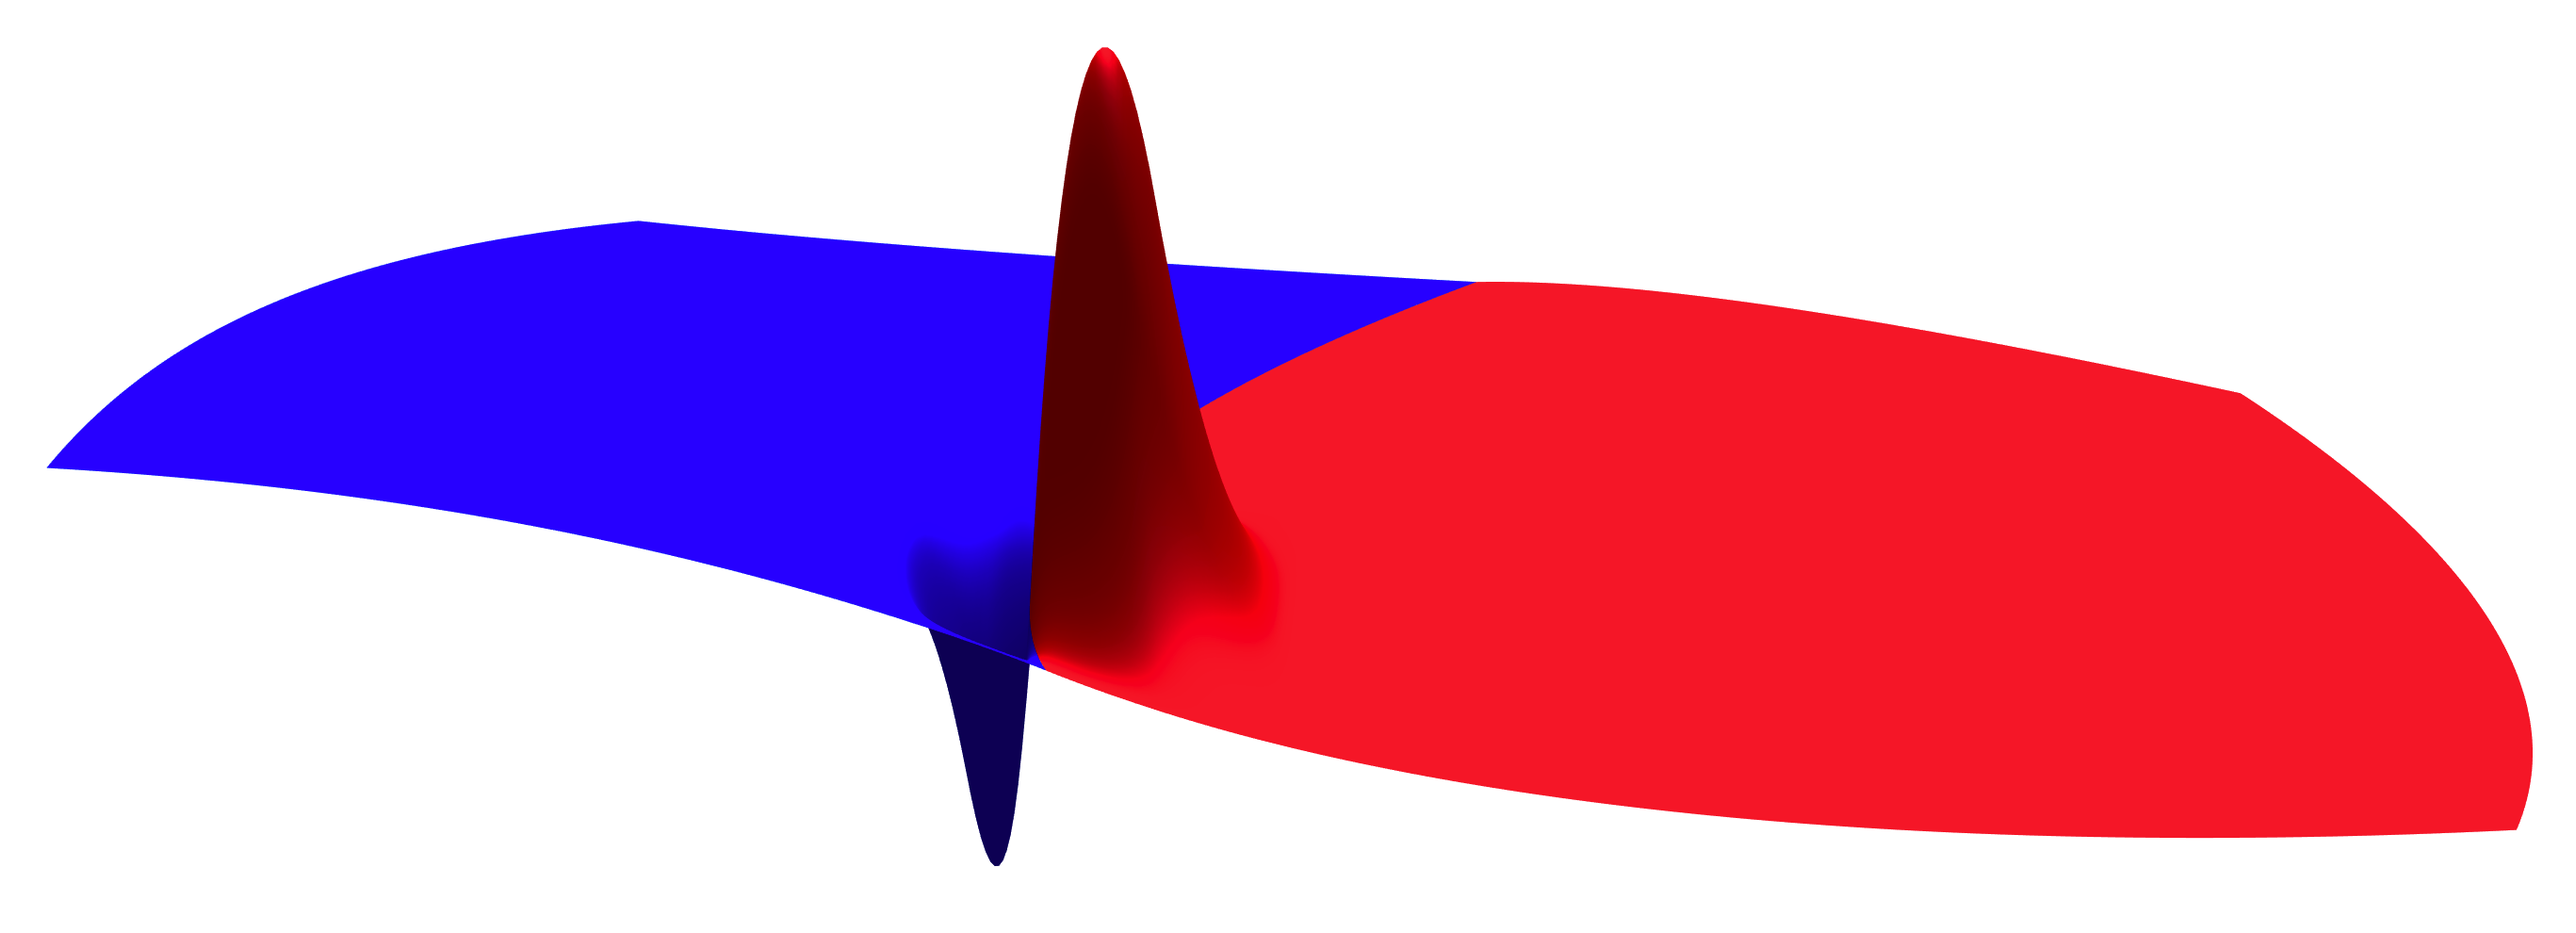
\includegraphics[scale=.15]{constrained_basis2}
  \end{subfigure}
  \hfill
  \begin{subfigure}[b]{0.47\textwidth}
    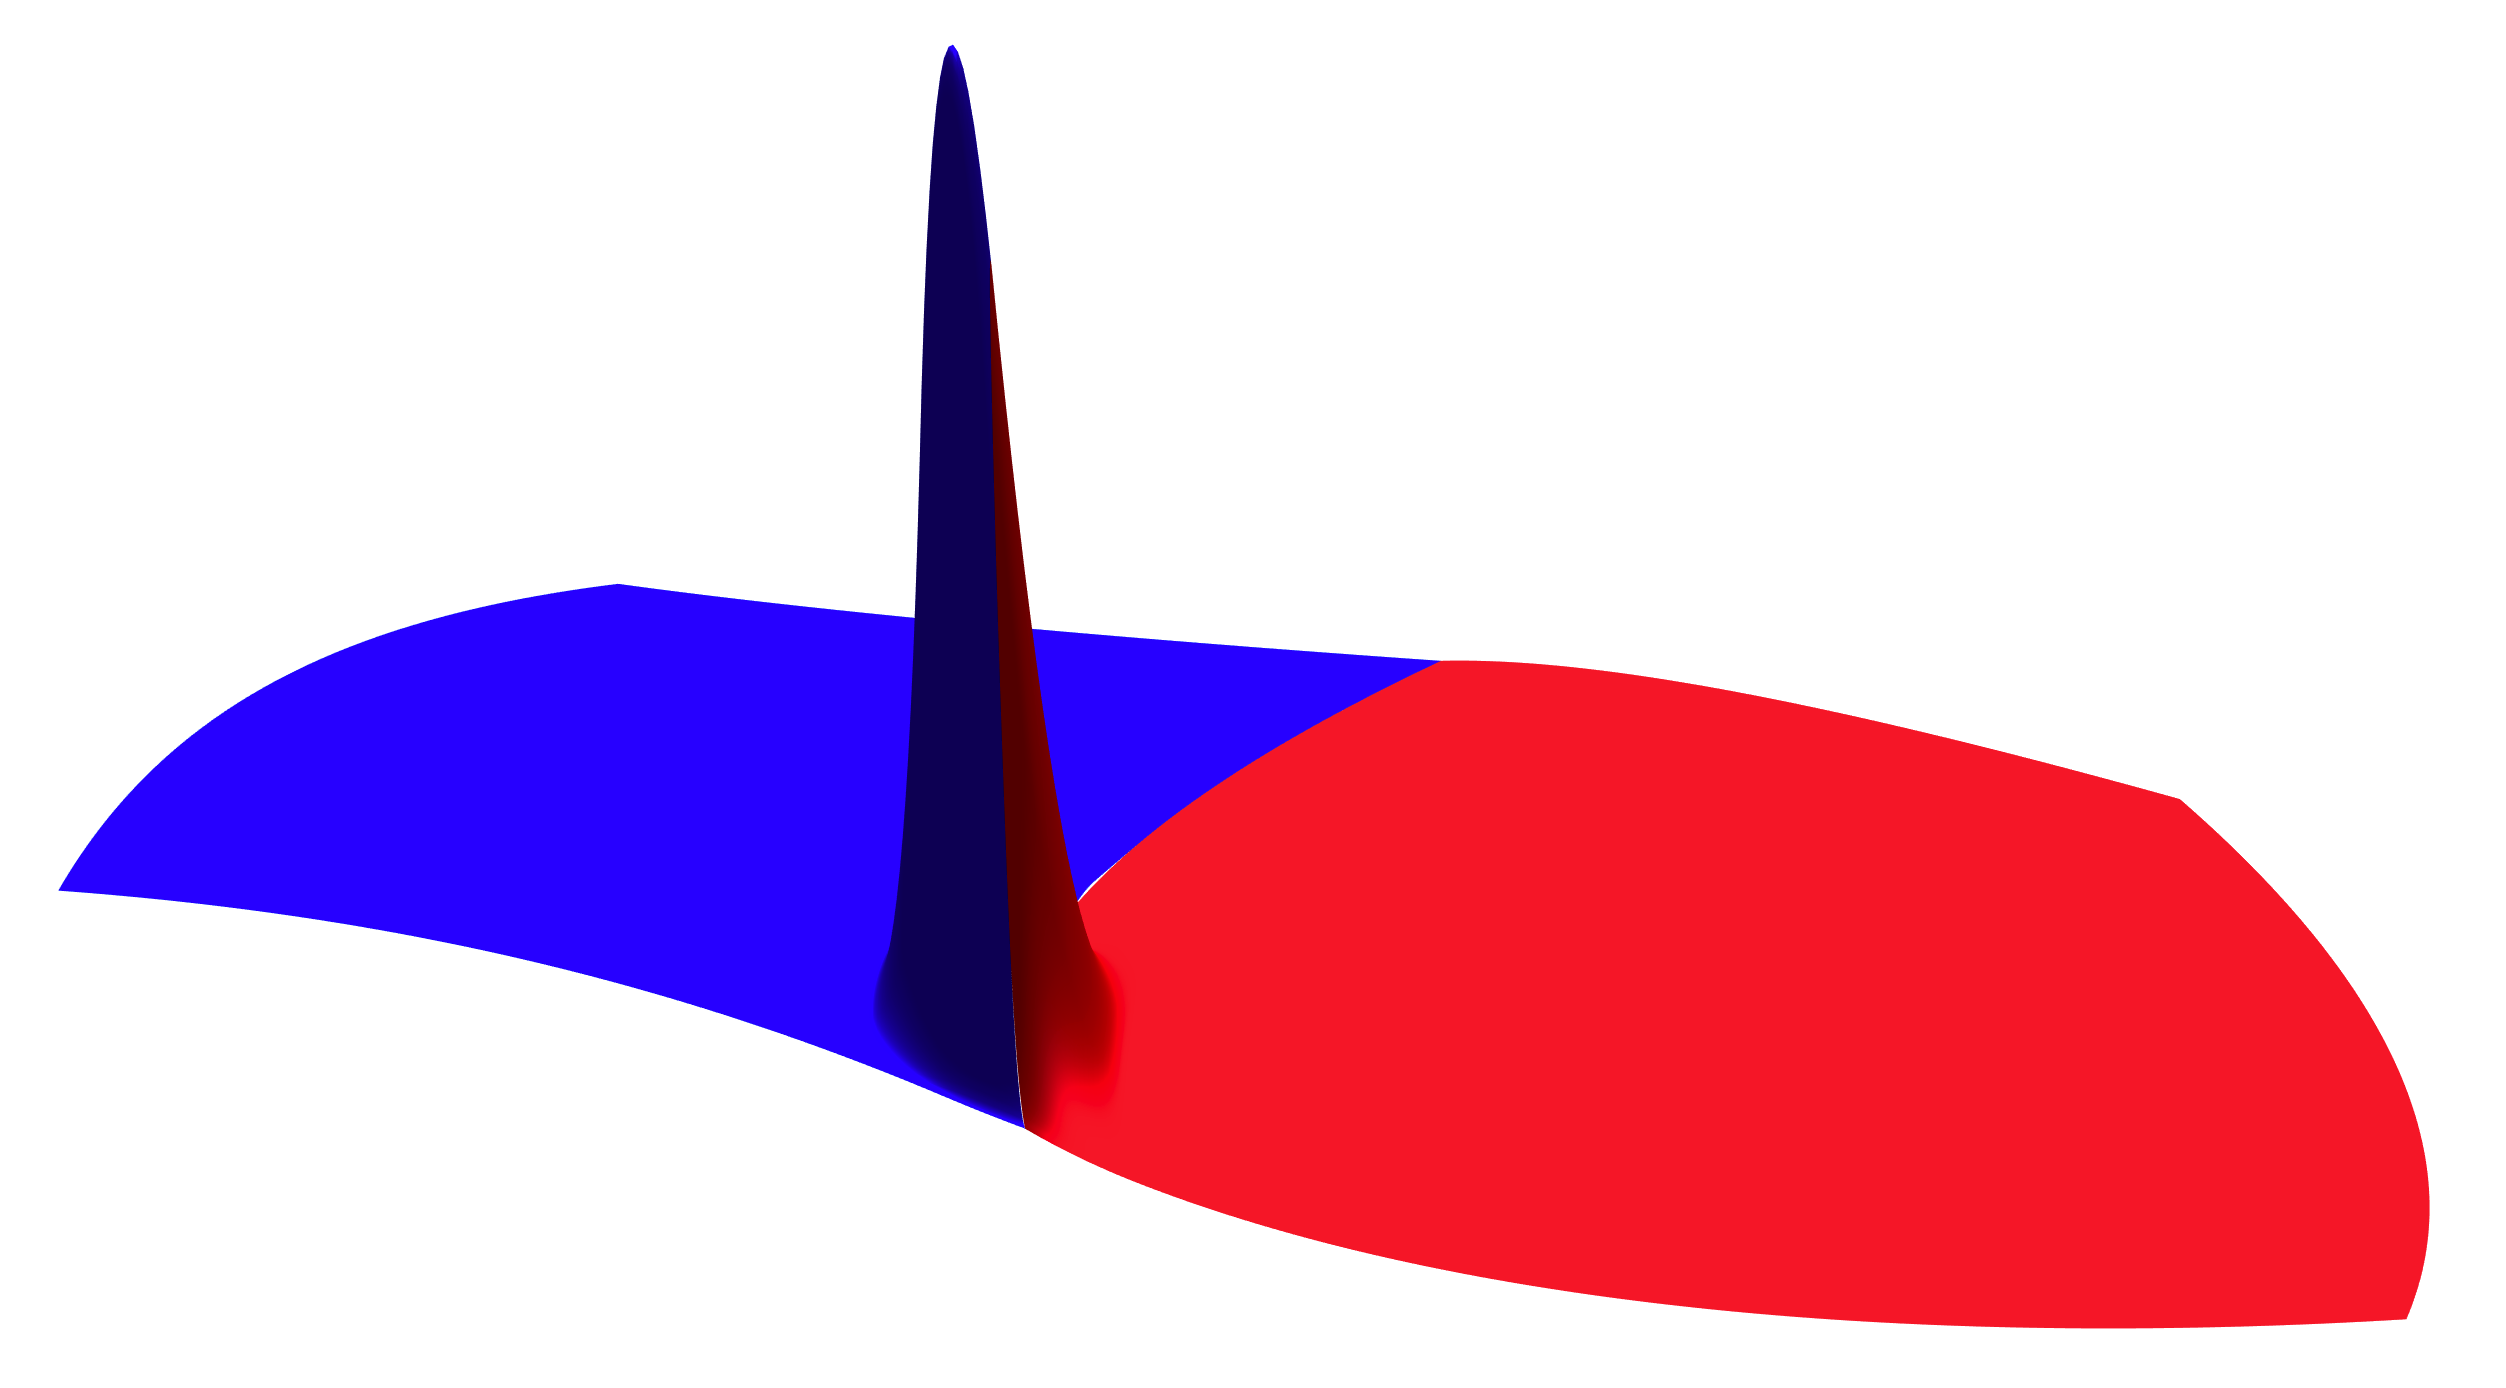
\includegraphics[scale=.15]{constrained_basis1}
  \end{subfigure}
  % or use \input{mytikz}
  \caption{Two exemplary basis functions in the constrained space $\mathcal{K}_b^h$.}
  \label{fig:constrained_basis}
\end{figure}

\subsection{The multi-patch case}

To extend this approach to more complex geometries requires the ability to stitch together multiple patches as shown in Figure~\ref{fig:three-patch-mesh}. To build the null space of a constraint matrix in the neighborhood of a vertex requires special care. From an implementation perspective, if we naively let the Lagrange multiplier spaces along all the interfaces adjacent to the vertex have the same dimension as the univariate spline basis along the slave side of the interface, there will be basis functions which serve as both slave and master. As an example, consider the the basis functions corresponding to the black pentagons of patch $\Omega_2$ in Figure~\ref{fig:three-patch-mesh}. As a result, there is no permutation under which the constraint matrix $\mathbf{B}$ can be modified to form~\eqref{eq:constraint-form} so that the basis of the null space can be found in a trivial way. Additionally, although the constraint matrices defined on each interface adjacent to a vertex are full row rank, the assembled constraint matrix $\mathbf{B}$ may not be full row rank. To overcome this problem, one may adopt matrix factorization techniques to solve the null space problem of a general constraint matrix $\mathbf{B}$, including LU, QR, SVD, etc. For example, a rank-revealing QR factorization of a rank-deficient constraint matrix $\mathbf{B}$ yields
\begin{equation}
  \mathbf{B}\mathbf{P}=
  \mathbf{Q}
  \begin{bmatrix}
    \mathbf{R}_1 & \mathbf{R}_2 \\
    \mathbf{0}   & \mathbf{0}
  \end{bmatrix}
\end{equation}
where $\mathbf{P}$ is a permutation matrix, $\mathbf{Q}$ is a unitary matrix, $\mathbf{R}_1$ is an upper triangular matrix and $\mathbf{R}_2$ is a rectangular matrix. The vector basis of the null space can then be taken to be
\begin{equation}
  \mathbf{C}=
  \mathbf{P}
  \begin{bmatrix}
    -\mathbf{R}_1^{-1}\mathbf{R}_2 \\
    \mathbf{I}
  \end{bmatrix}.\label{eq:direct_kernel}
\end{equation}
This type of global factorization has been utilized for patch coupling problems in~\cite{coox_robust_2017, coox2017flexible, dornisch2017dual}. However, it requires a global factorization of the entire constraint matrix $\mathbf{B}$, and fails to leverage the local properties of the dual basis. Moreover, the sparsity of the resulting constrained stiffness matrix might be negatively impacted since the inverse of $\mathbf{R}_1$ is a dense matrix. Additionally, \textit{inf-sup} stability may be violated and pathologies can be activated such as spurious oscillations and locking~\cite{barbosa1991finite}. For $2^\text{nd}$ order problems, one approach is to reduce the polynomial order of elements adjacent to vertices by one~\cite{bernardi_domain_1993,bernardi_basics_2005,belgacem_mortar_1998,brivadis_isogeometric_2015}. Then the modified Lagrange multiplier discretization is a subspace of the trace space of the slave patch of codimension $2$. By reducing the number of constraints, the basis functions in the neighborhood of vertices can now be considered masters. In addition, the modified Lagrange multiplier discretization is \textit{inf-sup} stable.\par

We introduce a sixth kind of B-spline basis function near a vertex $v\in \mathbf{V}$,
\begin{enumerate}
  \setcounter{enumi}{5}
  \item The basis function $N_i$ such that $\supp{N_i}\bigcap{v}\neq{}0$, or $\supp{\frac{\partial{}N_i}{\partial\xi}}\bigcap{v}\neq{}0$,  or $\supp{\frac{\partial{}N_i}{\partial\eta}}\bigcap{v}\neq{}0$ or $\supp{\frac{\partial^2{}N_i}{\partial\xi\partial\eta}}\bigcap{v}\neq{}0$, whose indices are denoted by the index set $I_\text{vi}$ (denoted by black pentagons in Figure~\ref{fig:three-patch-mesh}).
\end{enumerate}
The definitions of the other five kinds of B-spline basis functions remain the same except that their intersection with the sixth kind are excluded, that is
\begin{equation}
  I_k=I_k-I_\text{vi}\bigcap{}I_k, \quad k\in\{\text{i},\text{ii},\dots,\text{v}\}.
\end{equation}

\begin{figure}[ht]
  \center
  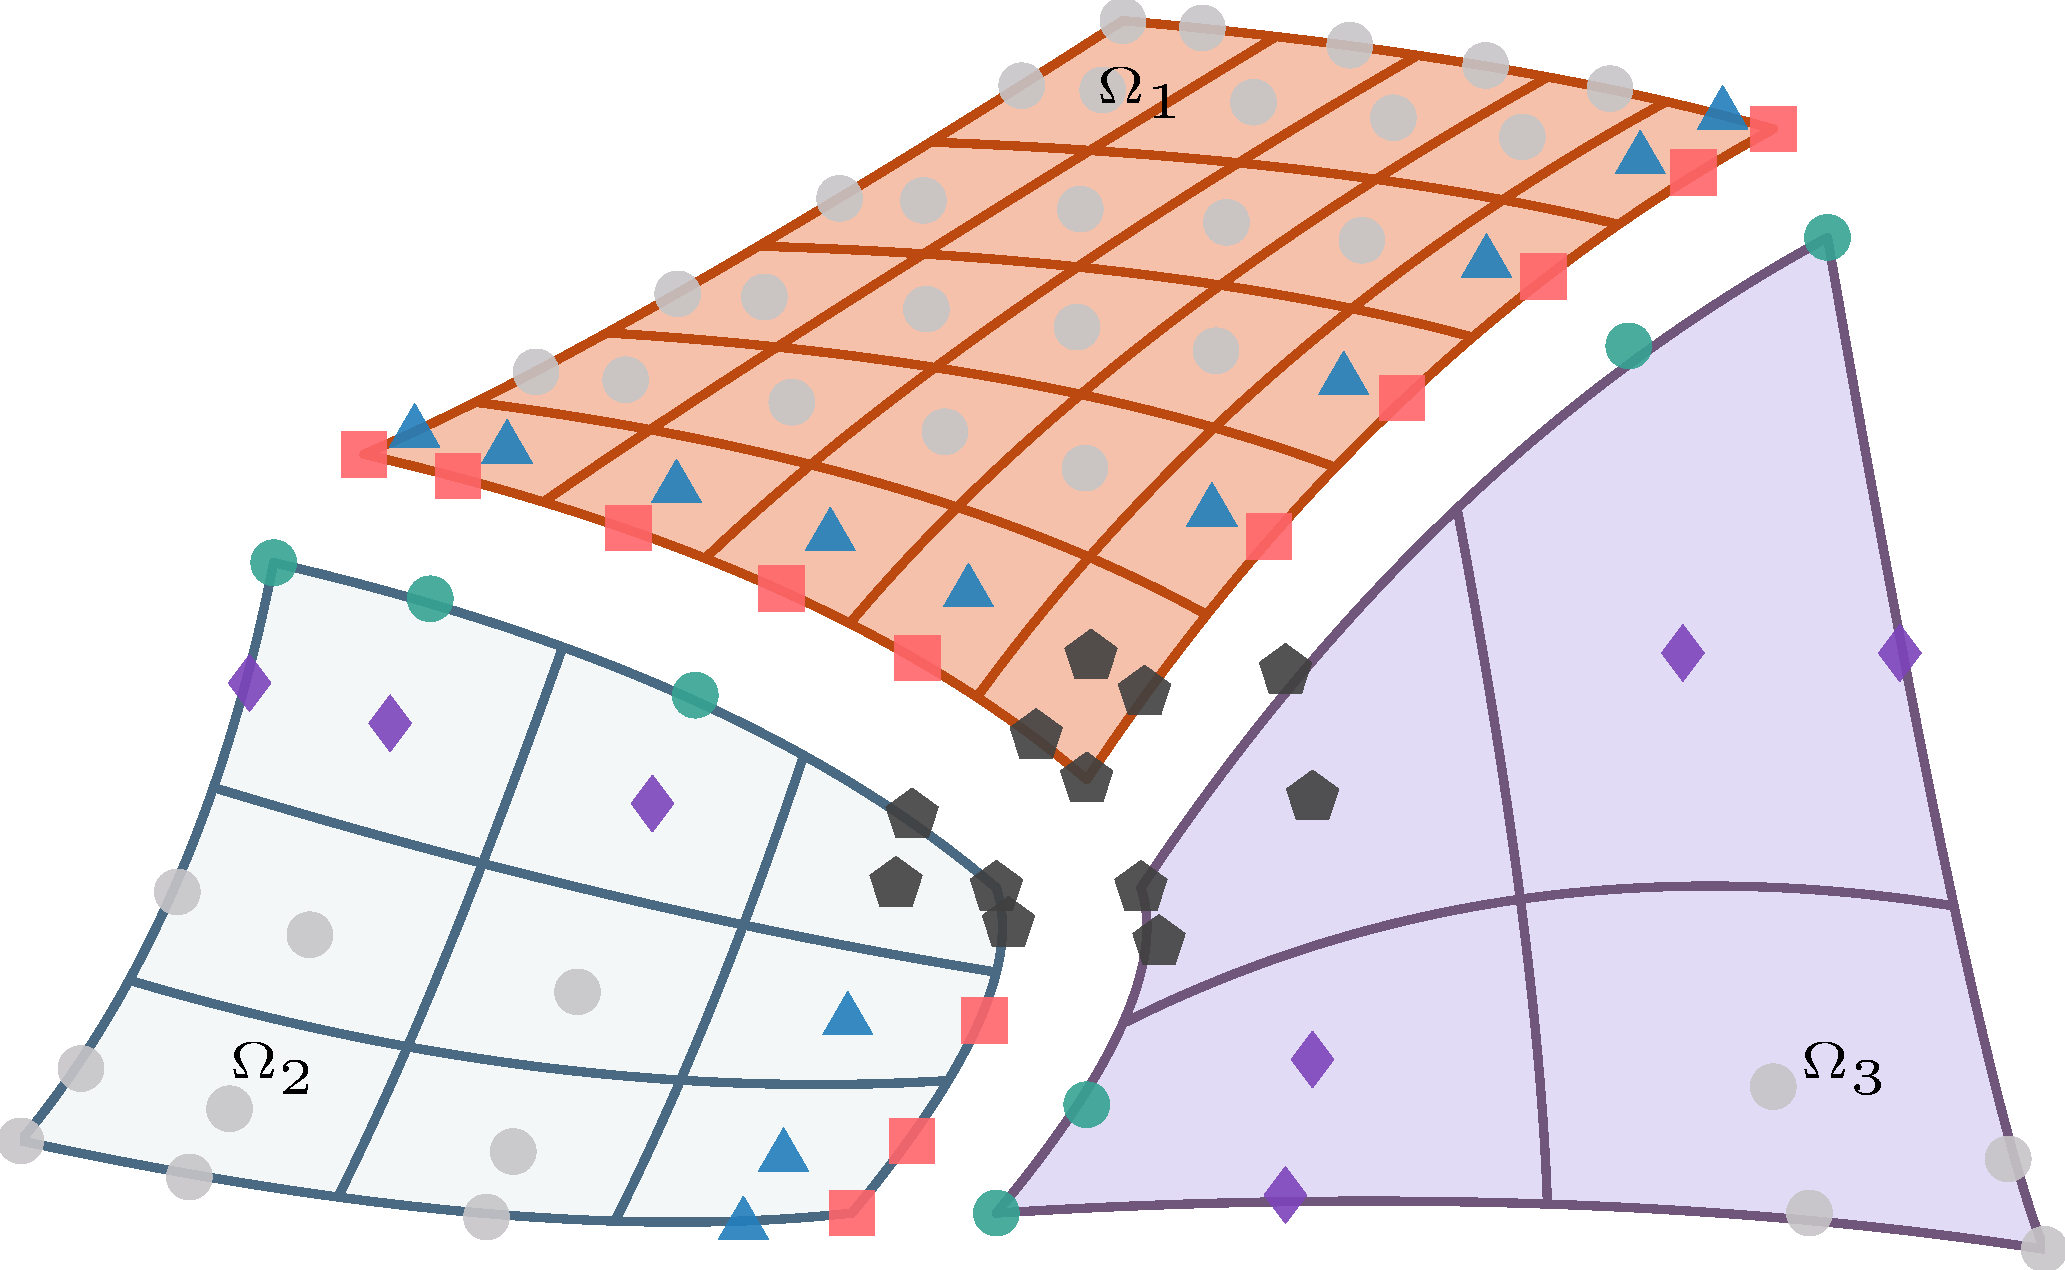
\includegraphics[scale=.4]{three-patch-mesh_backup}
  % or use \input{mytikz}
  \caption{A three-patch planar domain $\Omega$ consisting of $\Omega_1$, $\Omega_2$ and $\Omega_3$.}
  \label{fig:three-patch-mesh}
\end{figure}

\subsubsection{Global dual basis multi-patch treatment}\label{sec:vertex_modification}
In this approach, we reduce the number of constraints on each interface such that all of the sixth kind of B-spline basis functions can be classified as masters. For the biharmonic problem this requires a reduction of four constraints per vertex per patch. We accomplish this by coarsening the mesh in the neighborhood of each vertex. Specifically, we remove the two knots adjacent to each vertex. An example of this coarsening procedure for cubic univariate B-spline basis functions is shown in Figure~\ref{fig:boundary_modification}. The corresponding global dual basis can then be constructed by using~\eqref{eq:global_dual}. For a set of B-spline basis functions $\left\{N_i\right\}_{i=1}^n$ and the corresponding coarsened global dual basis $\left\{\hat{N}^G_i\right\}_{i=1}^{n-4}$, the biorthogonality relation is then given as
\begin{equation}
  \int_\Gamma \hat{N}^G_iN_{j+2} d\Gamma = \delta_{ij}, \quad \forall 1\leq i,j-2\leq n-4.\label{eq:modify_biorthogonality}
\end{equation}
In other words, the biorthogonality relation holds for all but the two basis functions nearest the vertices.\par

\begin{figure}[ht]
  \centering
  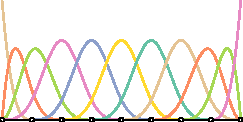
\includegraphics[width=.4\linewidth]{basis_original}\\
  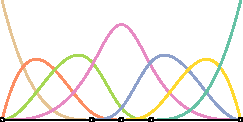
\includegraphics[width=.4\linewidth]{basis_coarse}
  \caption{A coarsening procedure for cubic B-spline basis functions. Top: original cubic basis functions. Bottom: basis functions of the coasened mesh, where two knots on each end are removed.}\label{fig:boundary_modification}
\end{figure}

A column-wise permutation matrix $\mathbf{P}_c$ which handles the multi-patch case can be defined as
\begin{equation}
  \begin{bmatrix}
    \mathbf{I}_\text{i}   \\
    \mathbf{I}_\text{ii}  \\
    \mathbf{I}_\text{iii} \\
    \mathbf{I}_\text{iv}  \\
    \mathbf{I}_\text{v}   \\
    \mathbf{I}_\text{vi}
  \end{bmatrix}=
  \mathbf{P}_c
  \begin{bmatrix}
    \mathbf{I}_1 \\
    \mathbf{I}_2 \\
    \vdots
  \end{bmatrix}.
\end{equation}
With the help of a row-wise permutation matrix, $\mathbf{P}_r$, the permuted constraint matrix can be written in the partitioned form
\begin{equation}
  \mathbf{B}^\text{mod}_p:=\mathbf{P}_r\mathbf{B}^\text{mod}_b\mathbf{P}_c^T=
  \begin{bmatrix}
    {\mathbf{B}}_1^1 & {\mathbf{B}}_1^2 & {\mathbf{B}}_1^3 & {\mathbf{B}}_1^4 & \mathbf{0} & {\mathbf{B}}_1^6 \\
    \mathbf{0}       & {\mathbf{B}}_2^2 & {\mathbf{B}}_2^3 & \mathbf{0}       & \mathbf{0} & {\mathbf{B}}_2^6
  \end{bmatrix},\label{eq:cross_point_constraint_structure}
\end{equation}
where $\mathbf{B}^\text{mod}_b$ is the constraint matrix constructed from the coarsened dual basis, $\mathbf{B}_1^1$ is the contribution of the first type of B-spline basis function in the discretization of $b_1$, and $\mathbf{B}_2^2$ is the contribution of the second type of B-spline basis function in the discretization of $b_0$. Under the row-wise permutation matrix $\mathbf{P}_r$, $\mathbf{B}_1^1$ and $\mathbf{B}_2^2$ become identity submatrices. Note that in the multi-patch case, basis functions in the neighborhood of in-domain vertices are excluded from the definitions of the first four types of B-spline basis functions. As a result, there is no basis function that will serve as both slave and master. As for the two patch case, the vector basis of the null space of $\mathbf{B}^\text{mod}_b$, denoted by $\mathbf{C}^\text{mod}_b$, can now be obtained from Equation~\eqref{eq:permuted_back_nullspace}, with
\begin{equation}
  \mathbf{C}^\text{mod}_p =
  \left[\begin{array}{cccc}
      {\mathbf{B}}_1^2{\mathbf{B}}_2^3-{\mathbf{B}}_1^3 & -{\mathbf{B}}_1^4 & \mathbf{0} & -{\mathbf{B}}_1^6 \\
      -{\mathbf{B}}_2^3                                 & \mathbf{0}        & \mathbf{0} & -{\mathbf{B}}_2^6 \\ \hdashline[2pt/2pt]
      \multicolumn{4}{c}{\multirow{3}{*}{\raisebox{0mm}{\scalebox{1.5}{$\mathbf{I}$}}}}                      \\
                                                        &                   &            &
    \end{array}\right].\label{eq:nullspace_modification}
\end{equation}

\begin{figure}[ht]
  \centering
  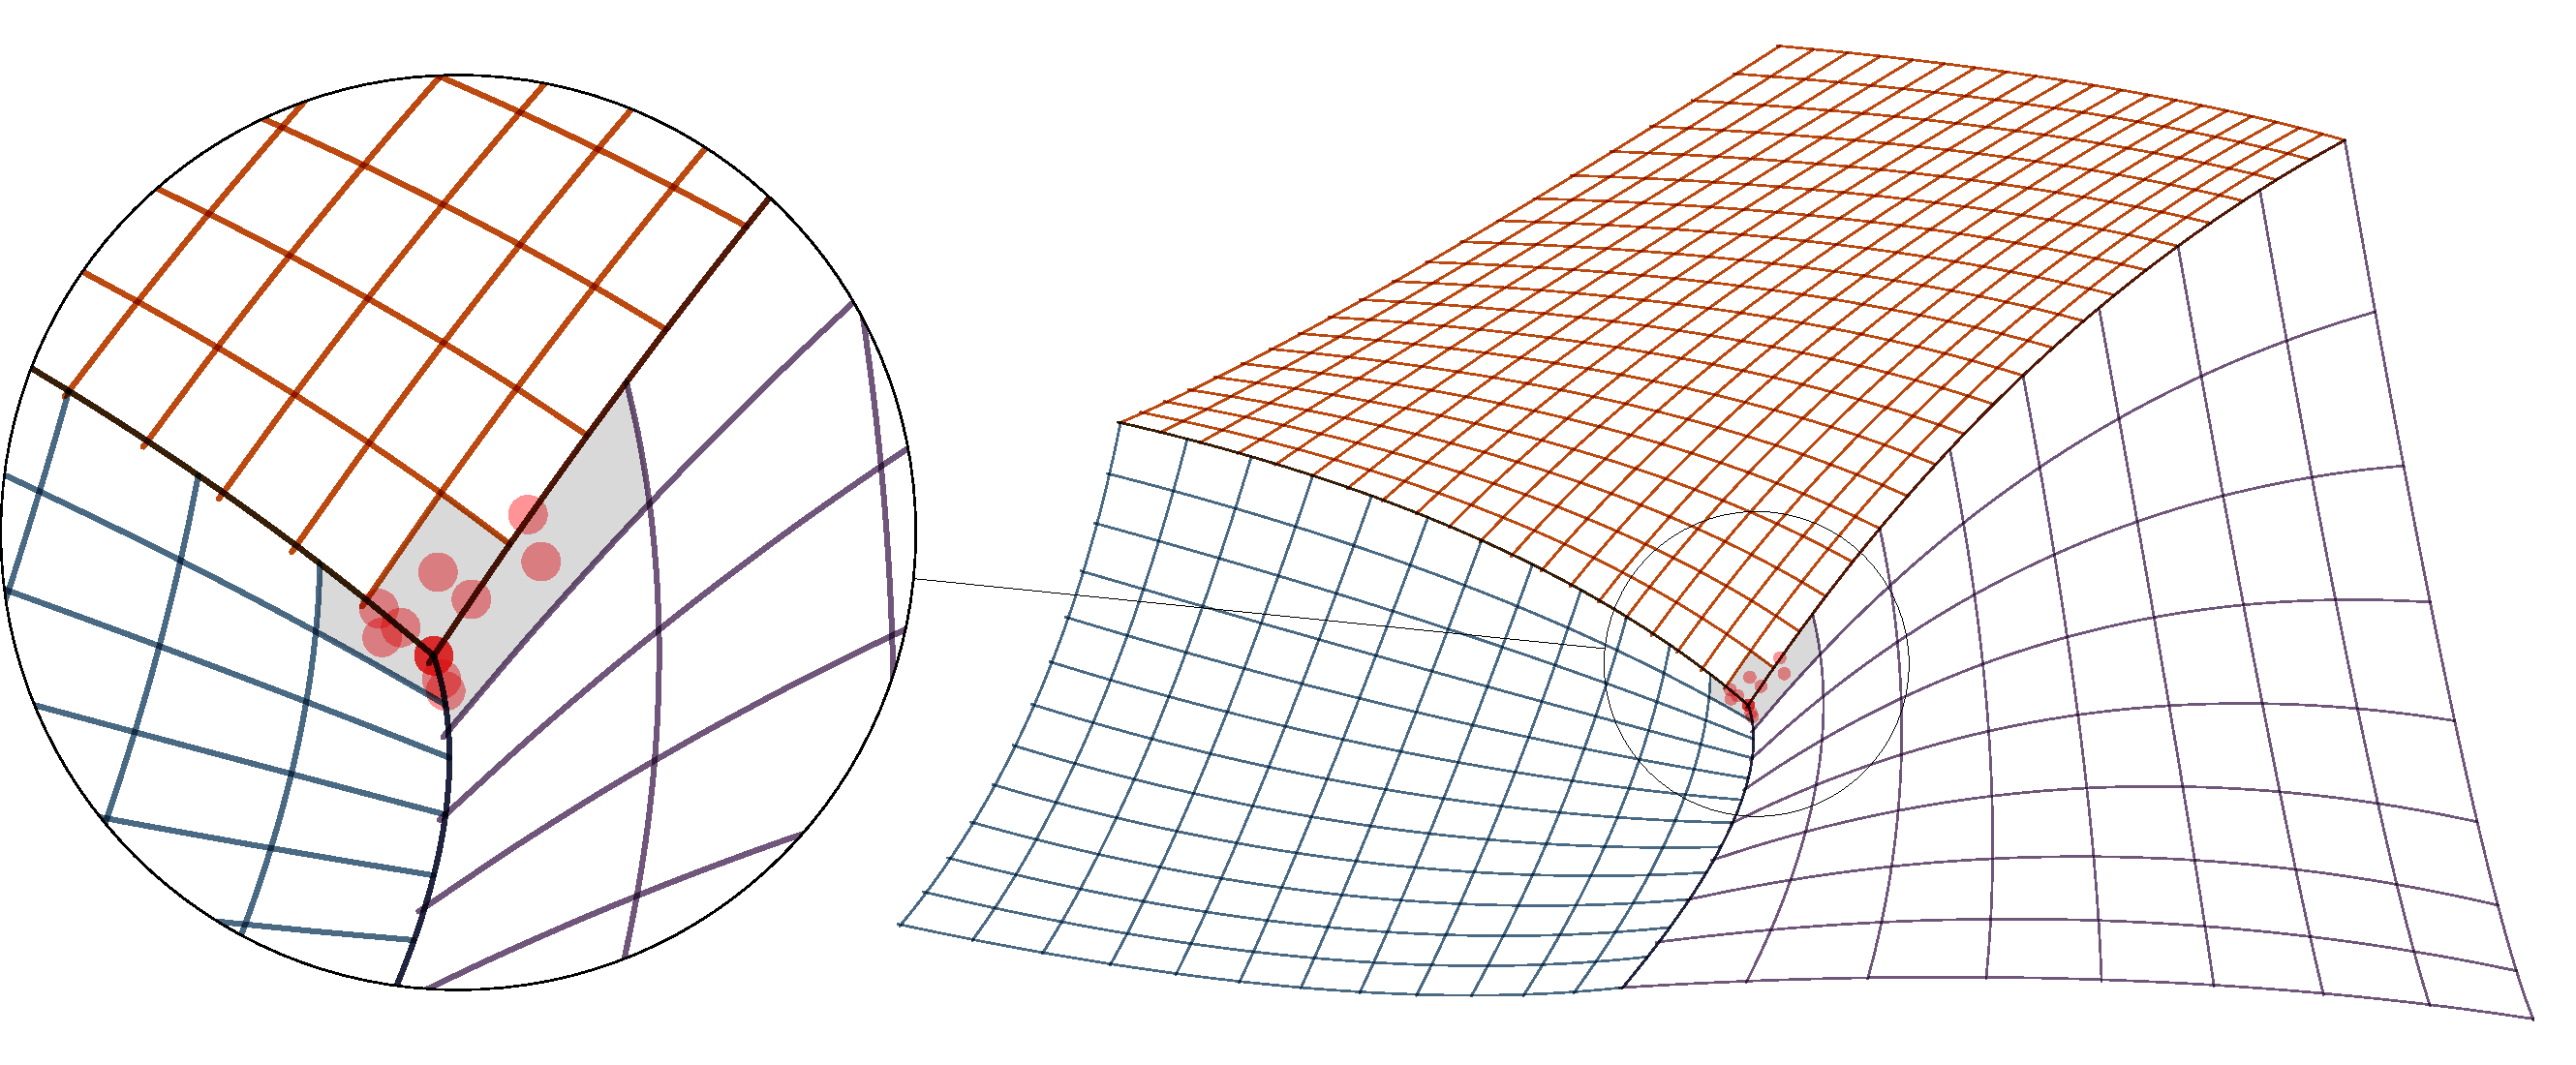
\includegraphics[width=\linewidth]{mesh_spy_modify}
  \caption{The degrees of freedom (red dots) involved in the constraint matrix $\mathbf{B}_v$ in section~\ref{sec:vertex_modification}.}\label{fig:cross_point_dof_modify}
\end{figure}

In order to guarantee the well-posedness of the mortar formulation and to improve the approximation, we further apply two continuity constraints at each vertex
\begin{equation}
  \left\{\begin{split}
    &u_s(v) = u_m(v)\\
    &\frac{\partial u_s(v)}{\partial \xi_s} = \frac{\partial u_m(v)}{\partial \xi_s}\text{ if }\Gamma\parallel\eta_s\text{ or }\frac{\partial u_s(v)}{\partial \eta_s} = \frac{\partial u_m(v)}{\partial \eta_s}\text{ if }\Gamma\parallel\xi_s
  \end{split}\right.,\label{eq:vertex_constraint}
\end{equation}
where $v$ is the position of a vertex. The matrix form of the pointwise constraints~\eqref{eq:vertex_constraint} is denoted by $\mathbf{B}_v$. Hence, in the presence of in-domain vertices, the constraint matrix $\mathbf{B}_b$ is formed from both applying constraints weakly through the coarsened dual basis functions along each interface and by applying constraints strongly at each vertex as
\begin{equation}
  \mathbf{B}_b =
  \begin{bmatrix}
    \mathbf{B}_v \\
    \mathbf{B}^\text{mod}_b
  \end{bmatrix}.
\end{equation}
The null space of $\mathbf{B}_b$ is the intersection of the null space of $\mathbf{B}_v$ and the null space of $\mathbf{B}^\text{mod}_b$. As a result, $\mathbf{C}_b$ is the vector basis of the null space of $\mathbf{B}_v$ constructed from $\Ima\mathbf{C}^\text{mod}_b$. First, we split the column vectors of $C^\text{mod}_b$ into two matrices
\begin{equation}
  \begin{split}
    \mathbf{C}_1&:=\{\mathbf{v}\in\mathbf{C}^\text{mod}_b\colon{\mathbf{B}_v\mathbf{v}={0}}\},\\
    \mathbf{C}_2&:=\{\mathbf{v}\in\mathbf{C}^\text{mod}_b\colon{\mathbf{B}_v\mathbf{v}\neq{0}}\}.
  \end{split}
\end{equation}
An example of this split is given in Figure~\ref{fig:overlap_nonoverlap_modify}. $\mathbf{C}_1$ contains vectors of $\mathbf{C}^\text{mod}_b$ that are also in the null space of $\mathbf{B}_v$. Thus, they contribute to part of $\mathbf{C}_b$. The null space of $\mathbf{B}_v$ from $\Ima \mathbf{C}_2$ can be constructed as $\mathbf{C}_2\bar{\mathbf{C}}$, where $\bar{\mathbf{C}}$ is the vector basis of the null space of $\bar{\mathbf{B}} = \mathbf{B}_v\mathbf{C}_2$ and can be constructed through the factorization in~\eqref{eq:direct_kernel}. Since for each patch, only at most four degrees of freedom per vertex per patch are involved in the formulation of $\mathbf{B}_v$ (see Figure~\ref{fig:cross_point_dof_modify}), the number of vectors in $\mathbf{C}_2$ is very small and the cost of the factorization of $\bar{\mathbf{B}}$ is negligible. The vector basis of the null space of $\mathbf{B}_b$ can now be given as
\begin{equation}
  \mathbf{C}_b =
  \begin{bmatrix}
    \mathbf{C}_1 & \mathbf{C}_2\bar{\mathbf{C}}\label{eq:c_b_matrix}
  \end{bmatrix}.
\end{equation}

\begin{figure}[ht]
  \centering
  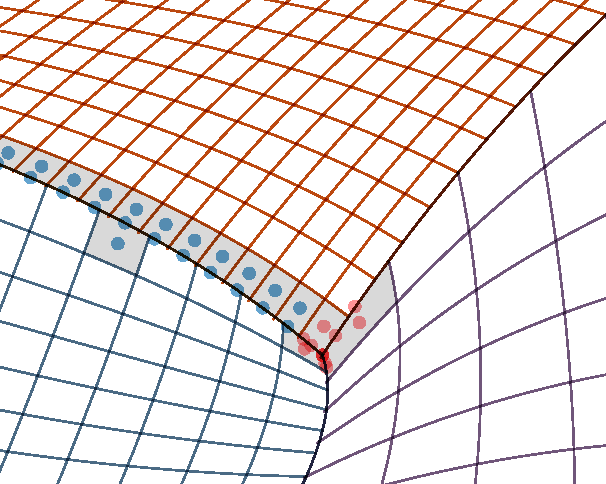
\includegraphics[width=.47\linewidth]{trim_nonoverlap_modify}\qquad
  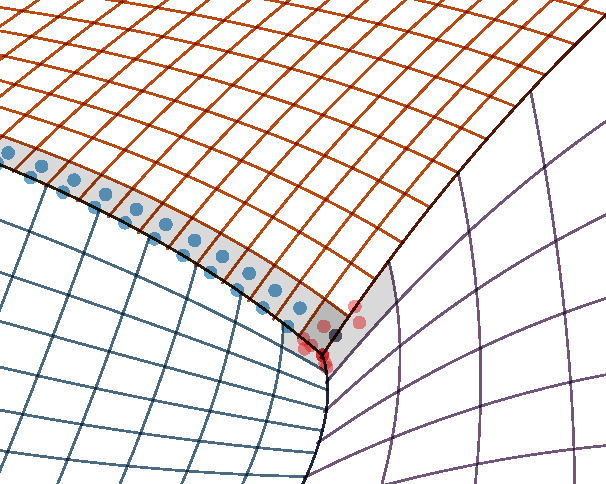
\includegraphics[width=.47\linewidth]{trim_overlap_modify}
  \caption{Activated degrees of freedom of the vector basis (blue) defined by the columns of $\mathbf{C}_b^\text{mod}$. Left: A vector basis classified as $\mathbf{C}_1$; Right: A vector basis classified as $\mathbf{C}_2$}\label{fig:overlap_nonoverlap_modify}
\end{figure}

\begin{remark}
  The \Bezier dual basis can also be coarsened by replacing the three closest basis functions at each vertex by their summation. In other words, for a set of \Bezier dual basis functions $\{\hat{N}^B_i\}_{i=1}^n$, the coarsened \Bezier dual basis functions $\{\hat{N}^\text{mod}_i\}_{i=1}^{n-4}$ are defined as follows
  \begin{equation}
    \hat{N}^\text{mod}_i=
    \begin{cases}
      \hat{N}^B_1+\hat{N}^B_2+\hat{N}^B_3\quad           & i=1,              \\
      \hat{N}^B_{n}+\hat{N}^B_{n-1}+\hat{N}^B_{n-2}\quad & i=n-4,            \\
      \hat{N}^B_{i+3}\quad                               & \text{otherwise}.
    \end{cases}\label{eq:bezier_dual_modification}
  \end{equation}
  This modification preserves the biorthogonality relation~\eqref{eq:modify_biorthogonality}. However, as can be seen from numerical examples, the modified \Bezier dual basis demonstrate poor performance. Hence, in the next subsection, we will introduce a multi-patch treatment for \Bezier dual basis functions without resorting to a modification at each vertex.
\end{remark}

\subsubsection{\Bezier dual basis multi-patch treatment}\label{sec:original_dual_basis}

In this approach, the basis functions in the discrete Lagrange multiplier spaces $\mathcal{M}^h_0$ and $\mathcal{M}^h_1$ are classified according to their proximity to a vertex. The basis functions in $\mathcal{M}^{h}_v$ are those in both $\mathcal{M}^h_0$ and $\mathcal{M}^h_1$ whose values and derivatives are non-zero at a vertex. The remaining basis functions are put in $\mathcal{M}^{h}_\text{inter}$. The constraint matrix can then be written as
\begin{equation}
  \mathbf{B}_b =
  \begin{bmatrix}
    \mathbf{B}_v \\
    \mathbf{B}_\text{inter}
  \end{bmatrix}
\end{equation}
where $\mathbf{B}_v$ is the matrix form of $b_0$ and $b_1$ restricted to the functions in $\mathcal{M}^{h}_v$ and $\mathbf{B}_\text{inter}$ is the matrix form of $b_0$ and $b_1$ restricted to the functions in $\mathcal{M}^{h}_\text{inter}$. Note that $\mathbf{B}_\text{inter}$ has the same structure as $\mathbf{B}_b^\text{mod}$ in Section~\ref{sec:vertex_modification}. The basis vectors of the null space of $\mathbf{B}_\text{int}$ can be constructed from~\eqref{eq:nullspace_modification} and is denoted by $\mathbf{C}_\text{inter}$. Using the approach outlined in Section~\ref{sec:vertex_modification}, we construct the basis vectors of the null space of $\mathbf{B}_v$ from $\Ima \mathbf{C}_\text{inter}$. $\mathbf{C}_\text{inter}$ can also be split into two submatrices $\mathbf{C}_1$ and $\mathbf{C}_2$. However, owing to the fact that $\mathbf{B}_v$ is constructed variationally, slightly more degrees of freedom are involved than in the approach described in Section~\ref{sec:vertex_modification} (see Figure~\ref{fig:cross_point_dof}). However, thanks to the locality of the \Bezier dual basis, the number of vectors in $\mathbf{C}_2$ is fixed. An example of this split is given in Figure~\ref{fig:overlap_nonoverlap}. Following the same procedure as described in Section~\ref{sec:vertex_modification}, we can construct $\mathbf{C}_b$ from Equation~\eqref{eq:c_b_matrix}.

\begin{figure}[ht]
  \centering
  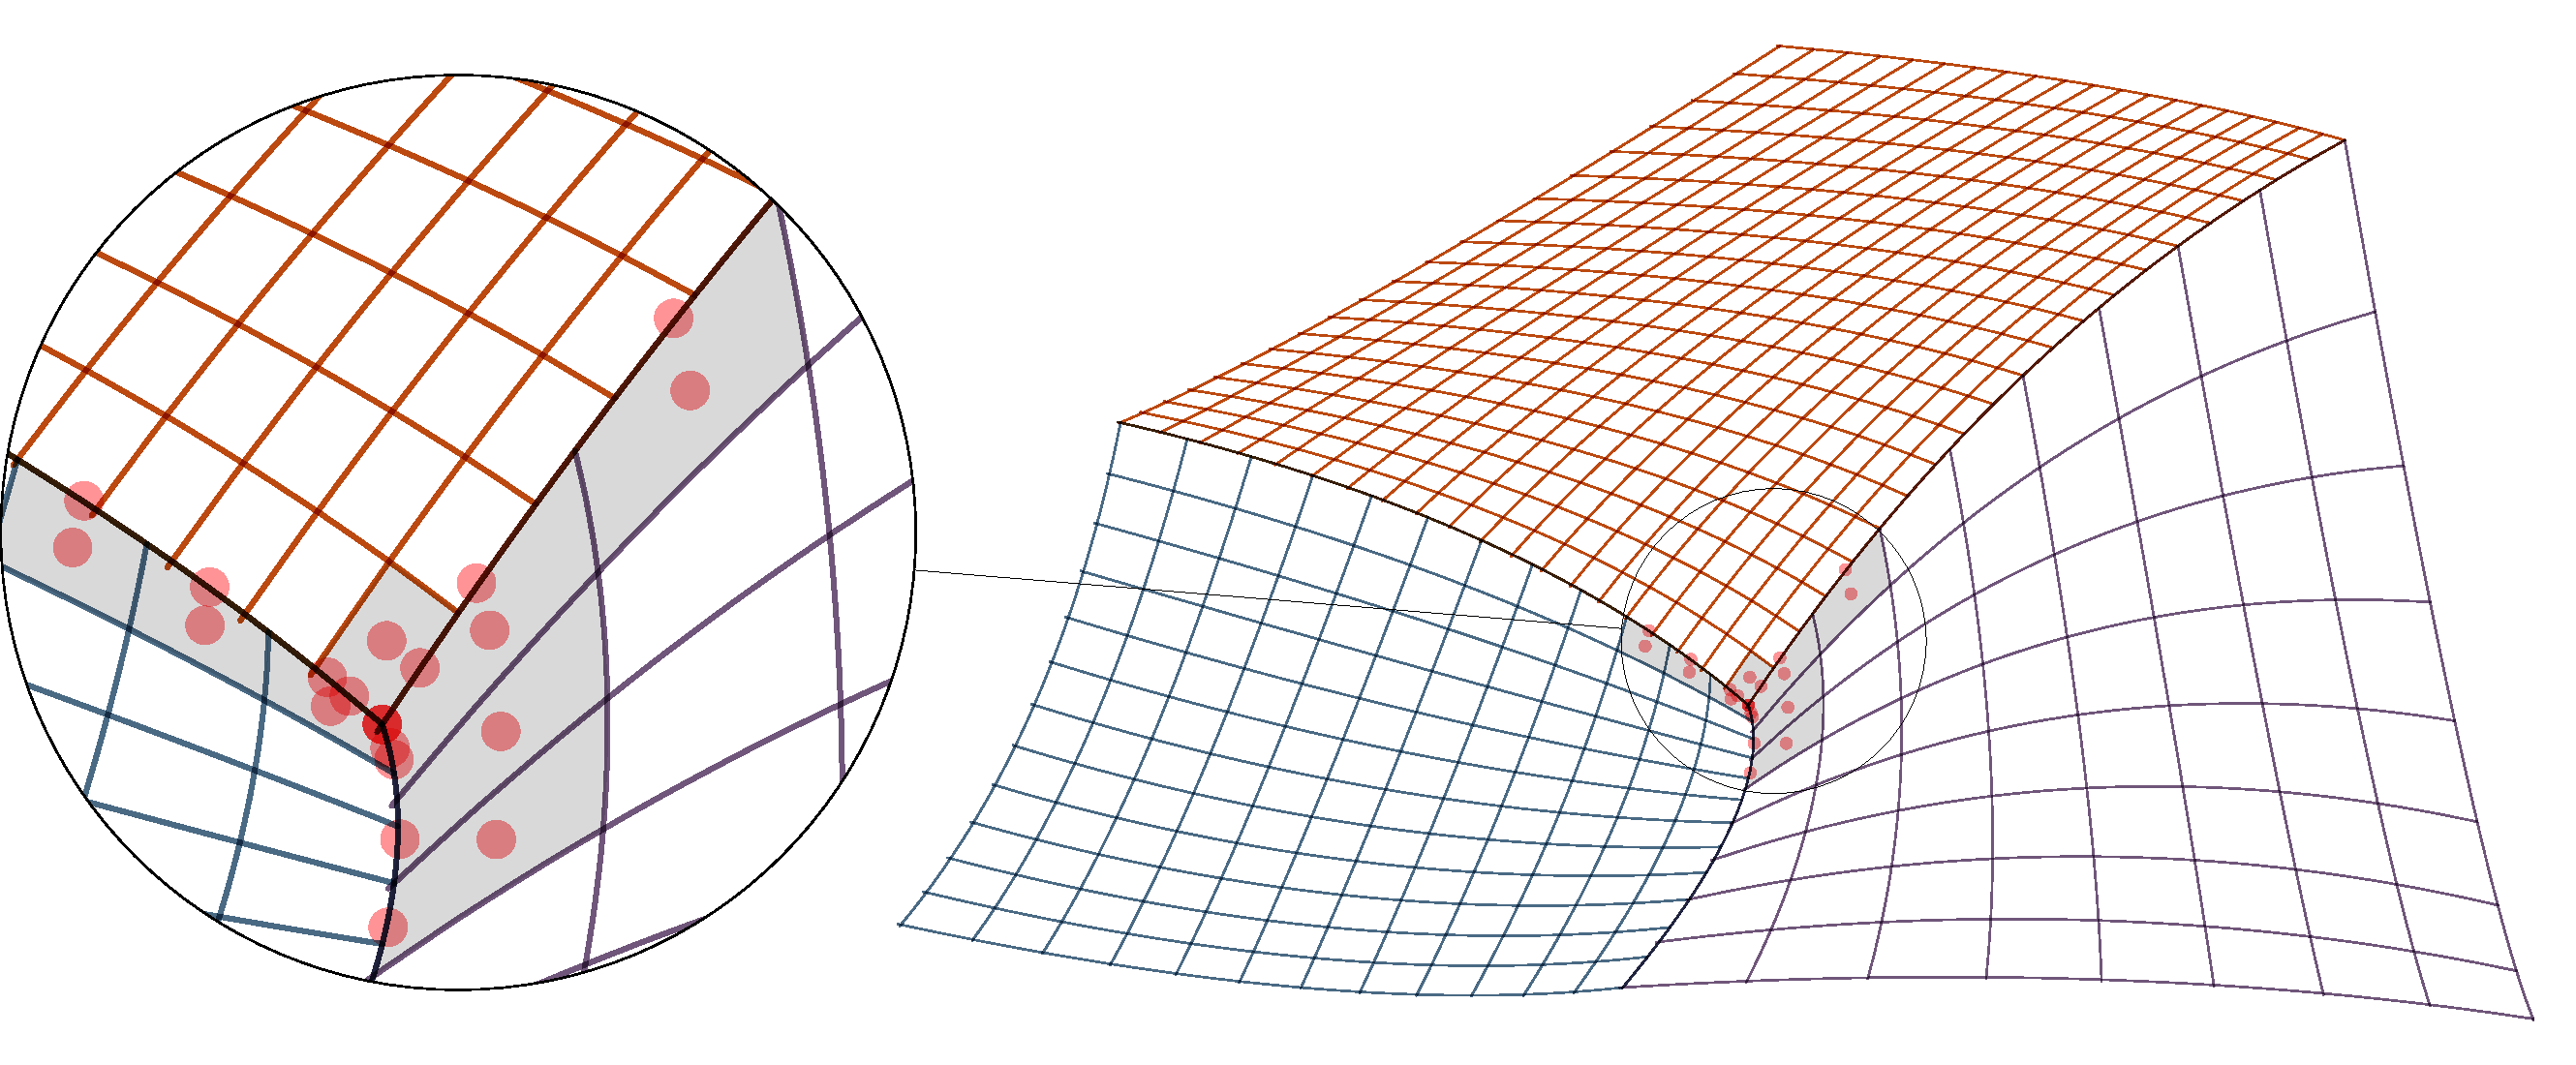
\includegraphics[width=\linewidth]{mesh_spy}
  \caption{The degrees of freedom (red dots) involved in the constraint matrix $\mathbf{B}_v$ in section~\ref{sec:original_dual_basis} formed from quadratic B-splines.}\label{fig:cross_point_dof}
\end{figure}

\begin{figure}[ht]
  \centering
  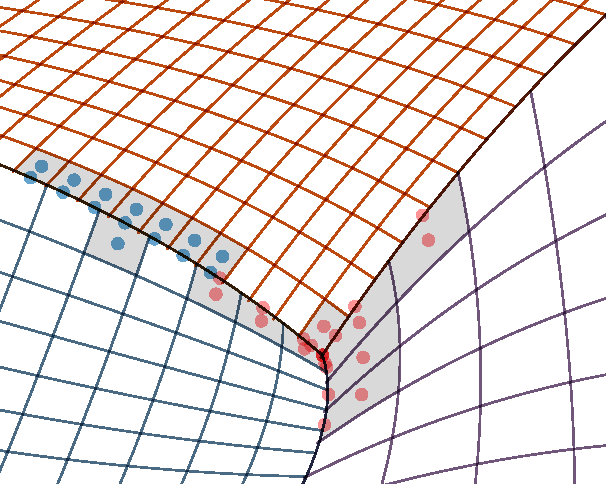
\includegraphics[width=.47\linewidth]{trim_nonoverlap}\qquad
  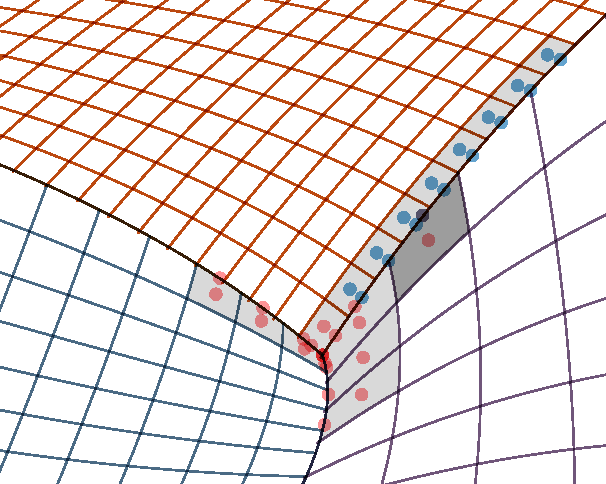
\includegraphics[width=.47\linewidth]{trim_overlap}
  \caption{Activated degrees of freedom of the vector basis (blue) defined by columns of $\mathbf{C}_\text{inter}$. Left: A vector basis classified as $\mathbf{C}_1$; Right: A vector basis classified as $\mathbf{C}_2$}\label{fig:overlap_nonoverlap}
\end{figure}

\begin{remark}
  This approach can be directly extended to the global dual basis as well. However, as can be seen from numerical examples, the global dual basis without the coarsening procedure is not inf-sup stable.
\end{remark}

\section{Finite element error analysis}\label{sec:error_analysis}

In this section, we study the finite element approximation of~\eqref{eq:biharmonic_mixed}. Suppose that $\mathcal{X}_b^h\subset{\mathcal{X}_b}$, $\mathcal{K}_b^h\subset{\mathcal{K}_b}$, $\mathcal{M}_0^h\subset{\mathcal{M}_0}$ and $\mathcal{M}_1^h\subset{\mathcal{M}_1}$ are finite-dimensional linear subspaces of the spaces $\mathcal{X}_b$, $\mathcal{K}_b$, $\mathcal{M}_0$, and $\mathcal{M}_1$.
\begin{lemma}\label{aspt:bounded-operator}
  (bounded above) The bilinear functionals $a_b(\cdot,\cdot)$, $b_0(\cdot,\cdot)$ and $b_1(\cdot,\cdot)$ are all bounded; i.e., there exists positive constants $C_a$, $C_{b_0}$ and $C_{b_1}$ such that
  \begin{align}
    \begin{split}
      \vert{a_b{(u,v)}}\vert&\leq{C_a\|u\|_{H^2_*}\|v\|_{H^2_*}},\\
      \vert{b_0{(\mu_0,u)}}\vert&\leq{C_{b_0}\|\mu_0\|_{H^{-\frac{3}{2}}}\|u\|_{H^2_*}},\\
      \vert{b_1{(\mu_1,u)}}\vert&\leq{C_{b_1}\|\mu_1\|_{H^{-\frac{1}{2}}}\|u\|_{H^2_*}},
    \end{split}
    \quad\quad
    \begin{split}
      \forall{u,v}&\in{\mathcal{X}_b},\\
      \forall{\mu_0}\in\mathcal{M}_0, {u}&\in{\mathcal{X}_b},\\
      \forall{\mu_1}\in\mathcal{M}_1, {u}&\in{\mathcal{X}_b}.
    \end{split}
  \end{align}

  \begin{proof}
    The continuity of $a_b(\cdot,\cdot)$ follows from the Cauchy-Schwarz inequality, the continuities of $b_0(\cdot,\cdot)$ and $b_1(\cdot,\cdot)$ follow from the definition of the dual norm and the trace theorem.
  \end{proof}
\end{lemma}

\begin{lemma}\label{aspt:coercive}
  (bounded below) The bilinear functional $a_b(\cdot,\cdot)$ is coercive on the space $\mathcal{K}^h_b$ that is constructed from both the global dual basis functions and the \Bezier dual basis functions, i.e.,
  \begin{equation}
    \exists{c_a>0}\;\text{that is independent of the mesh size $h$ such that}\,\,\forall{v^h}\in\mathcal{K}_b^h,\, a_b(v^h,v^h)\geq{c_a\|{v^h}\|_{H^2_*}}.\label{eq:coercive}
  \end{equation}
  \begin{proof}
    We introduce the function space $\bar{\mathcal{X}}_b$ as all functions in $\mathcal{X}_b$ that satisfy the pointwise constraint~\eqref{eq:vertex_constraint} on each vertex and are also $C^\infty$ in each patch. Then we have the following inclusion, $\mathcal{K}^h_b\subset \bar{\mathcal{X}}_b \subset  \mathcal{X}_b$. For the case of the \Bezier dual basis, the inclusion comes from~\eqref{eq:boundary_interpolation}; for the case of the global dual basis, the inclusion comes from the pointwise constraints at the vertex. We consider the coercivity of $a_b(\cdot,\cdot)$ on $\bar{\mathcal{X}}_b$. Suppose that this statement is false, then there exists a sequence $\{v_n\}_{n=1}^{\infty}\in \bar{\mathcal{X}}_b$ such that
    \begin{equation}
      \sum_{k=1}^K\vert v_n \vert_{H^2(\Omega_k)}\leq \frac{1}{n}\;\text{ and }\;\sum_{k=1}^K\| v_n \|_{H^2(\Omega_k)}=1.\label{eq:countrary}
    \end{equation}
    For any $1\leq k \leq K$, the sequence $\left\{ v_n\vert_{\Omega_k} \right\}_{n=1}^\infty$ is bounded in $H^2(\Omega_k)$. Hence, there exists a subsequence $\left\{ (v_n)_m\vert_{\Omega_k} \right\}_{m=1}^\infty$ such that
    \begin{equation}
      (v_n)_m\vert_{\Omega_k} \rightharpoonup v\vert_{\Omega_k} \text{weakly in } H^2(\Omega_k).
    \end{equation}
    By the Rellich-Kondrachov theorem, $\left\{ (v_n)_m\vert_{\Omega_k} \right\}_{m=1}^\infty$ converges to $v\vert_{\Omega_k}$ strongly in $H^1(\Omega_k)$. In other words,
    \begin{equation}
      \lim_{m\to\infty}\| (v_n)_m \vert_{\Omega_k} -v \vert_{\Omega_k}\|_{H^1(\Omega_k)}=0.
    \end{equation}
    From $\vert v_n \vert_{H^2(\Omega_k)}\rightarrow 0$, we have that $\left\{ (v_n)_m\vert_{\Omega_k} \right\}_{m=1}^\infty$ is a Cauchy sequence in $H^2(\Omega_k)$. Thus, we have that $v \vert_{\Omega_k}\in H^2(\Omega_k)$ and
    \begin{equation}
      \lim_{m\to\infty}\| (v_n)_m \vert_{\Omega_k} -v \vert_{\Omega_k}\|_{H^2(\Omega_k)}=0.
    \end{equation}
    From the approximation theory,
    \begin{equation}
      \inf_{r^k_n\in\mathcal{P}^1(\Omega_k)}\|v_{n}-r^k_n\|_{H^1(\Omega_k)}\leq C \vert v_{n} \vert_{H^2(\Omega_k)} \leq \frac{C}{n}
    \end{equation}
    where $\mathcal{P}^1(\Omega_k)$ is the $1^\text{st}$ order polynomial space on $\Omega_k$. Hence,
    \begin{equation}
      \| (r^k_n)_m-v\|_{H^1(\Omega_k)} \leq \| (r^k_n)_m-(v_n)_m\|_{H^1(\Omega_k)}+\| (v_n)_m-v\|_{H^1(\Omega_k)} \rightarrow 0.
    \end{equation}
    This means $v\vert_{\Omega_k}$ is a linear function on $\Omega_k$. If $\Omega_k$ is a boundary element (i.e. $\partial \Omega_k\bigcap \partial\Omega\neq\emptyset$), the only linear functions that satisfies the boundary condition is the zero function. Hence,
    \begin{equation}
      \|(v_{n})_m\|_{H^2(\Omega_k)}=\|(v_{n})_m-v\|_{H^2(\Omega_k)}\rightarrow 0.
    \end{equation}
    If patch $\Omega_l$ is coupled with $\Omega_k$ along the intersection $\Gamma_{kl}\parallel \eta_k$, then on both ends $a,b$ of $\Gamma_{kl}$ we have
    \begin{equation}
      v(a) = 0,\; v(b) = 0,\; \frac{\partial v(a)}{\partial \xi_k} = 0,\;\text{ and }\frac{\partial v(b)}{\partial \xi_k} = 0.\label{eq:boundary_conditions}
    \end{equation}
    Hence, $v\vert_{\Omega_l}=0$. Similar arguments can be applied to all patches, leading to
    \begin{equation}
      \sum_{k=1}^K\| (v_n)_m \|_{H^2(\Omega_k)}\rightarrow 0.
    \end{equation}
    This is inconsistent with~\eqref{eq:countrary}. As a result, \eqref{eq:coercive} holds.
  \end{proof}
\end{lemma}

\begin{theorem}
  There exists a unique solution $u^h\in{\mathcal{K}_b^h}$ that satisfies~\eqref{eq:weak-form} for all $v^h\in{\mathcal{K}_b^h}$, with $\mathcal{K}_b^h$ constructed using either the \Bezier or global dual basis.
  \begin{proof}
    Thanks to Lemma~\ref{aspt:bounded-operator} and Lemma~\ref{aspt:coercive}, the well-posedness of problem~\eqref{eq:weak-form} in $\mathcal{K}_b^h$ follows from the Lax-Milgram theorem~\cite{brenner_mathematical_2007}.\par
  \end{proof}
\end{theorem}

\begin{lemma}
  (Strang's lemma) Let $u\in H^2_0(\Omega)$ satisfy problem~\eqref{eq:weak-form} for all $v\in H^2_0(\Omega)$, then the error between $u$ and $u^h$ is given by
  \begin{equation}
    \|u-u^h\|_{H^2_*}\leq{\left(1+\frac{C_a}{c_a}\right)}\inf_{v^h\in{\mathcal{K}_b^h}}\|u-v^h\|_{H^2_*}+\frac{1}{c_a}\sup_{w^h\in \mathcal{K}_b^h\backslash \{0\}}\frac{\vert a_b(u-u^h,w^h) \vert }{\|w^h\|_{H^2_*}},
  \end{equation}
  where the first term on the righthand side is often called the approximation error and the second term is often called the consistency error.
  \begin{proof}
    See~\cite{brenner_mathematical_2007}.
  \end{proof}
\end{lemma}
From Strang's lemma, we may now obtain the following result by expanding the term $a_b(u-u^h,w^h)$.
\begin{theorem}\label{thm:fea-approx}
  The error between $u$ and $u^h$ is given by
  \begin{equation}
    \begin{split}
      \|u-u^h\|_{H^2_*}\leq &{\left(1+\frac{C_a}{c_a}\right)}\inf_{v^h\in{\mathcal{K}_b^h}}\|u-v^h\|_{H^2_*}+\frac{c_b}{c_a}\sum_{\Gamma\in \mathbf{S}}B,
    \end{split}
    \label{eq:fem_approximation}
  \end{equation}
  with
  \begin{equation}
    B= \left\{\begin{split}
      \inf_{\lambda_0^h\in \mathcal{M}_0^h}\| \frac{\partial \Delta u}{\partial \mathbf{n}} + r_{\eta_s} - \lambda_0^h \|_{H^{-\frac{3}{2}}(\Gamma)}+ \inf_{\lambda_1^h\in \mathcal{M}_1^h} \| \Delta u \frac{\partial \xi_s}{\partial \mathbf{n}} - \lambda_1^h \|_{H^{-\frac{1}{2}}(\Gamma)}\quad\quad &\Gamma\parallel \eta_s,\\
      \inf_{\lambda_0^h\in \mathcal{M}_0^h}\| \frac{\partial \Delta u}{\partial \mathbf{n}} + r_{\xi_s} - \lambda_0^h \|_{H^{-\frac{3}{2}}(\Gamma)}+ \inf_{\lambda_1^h\in \mathcal{M}_1^h} \| \Delta u \frac{\partial \eta_s}{\partial \mathbf{n}} - \lambda_1^h \|_{H^{-\frac{1}{2}}(\Gamma)}\quad \quad&\Gamma\parallel \xi_s,
    \end{split}\right.
  \end{equation}
  where
  \begin{equation}
    r_{\eta_s} = \partial_{\eta_s}\left(\Delta u \frac{\partial \eta_s}{\partial \mathbf{n}}\vert \Gamma' \vert\right)\frac{1}{\vert \Gamma' \vert},\quad r_{\xi_s} = \partial_{\xi_s}\left(\Delta u \frac{\partial \xi_s}{\partial \mathbf{n}}\vert \Gamma' \vert\right)\frac{1}{\vert \Gamma' \vert},
  \end{equation}
  with
  \begin{equation}
    \begin{split}
      \vert \Gamma' \vert = \sqrt{\frac{\partial x}{\partial \eta_s}^2+\frac{\partial y}{\partial \eta_s}^2}\quad\quad &\Gamma\parallel \eta_s\\
      \vert \Gamma' \vert = \sqrt{\frac{\partial x}{\partial \xi_s}^2+\frac{\partial y}{\partial \xi_s}^2}\quad\quad &\Gamma\parallel \xi_s
    \end{split}
  \end{equation}
  and $c_b$ is a constant independent of the mesh size.
  \begin{proof}
    Here we only discuss the stituation where $\Gamma\parallel \eta_s$. By Green's theorem, we have that
    \begin{equation}
      \begin{split}
        a_b(u-u^h,w^h)&=a_b(u, w^h)-\langle f,w^h \rangle_{\Omega}\\
        &=\langle \Delta^2u,w^h \rangle_{\Omega}+\sum_{\Gamma\in \mathbf{S}}\left(\int_\Gamma\Delta u\left[\frac{\partial{w^h}}{\partial \mathbf{n}}\right]_\Gamma d\Gamma - \int_\Gamma\frac{\partial \Delta u}{\partial \mathbf{n}}\left[{w^h}\right]_\Gamma d\Gamma\right)-\langle f,w^h \rangle_{\Omega}\\
        &=\sum_{\Gamma\in \mathbf{S}}\left(\int_\Gamma\Delta u\left[\frac{\partial{w^h}}{\partial \mathbf{n}}\right]_\Gamma d\Gamma - \int_\Gamma\frac{\partial \Delta u}{\partial \mathbf{n}}\left[{w^h}\right]_\Gamma d\Gamma\right)\\
        &=\sum_{\Gamma\in \mathbf{S}}\left(\int_\Gamma\Delta u \frac{\partial \xi_s}{\partial \mathbf{n}}\left[\frac{\partial{w^h}}{\partial \xi_s}\right]_\Gamma d\Gamma+\int_\Gamma\Delta u \frac{\partial \eta_s}{\partial \mathbf{n}}\left[\frac{\partial{w^h}}{\partial \eta_s}\right]_\Gamma d\Gamma-\int_\Gamma\frac{\partial \Delta u}{\partial \mathbf{n}}\left[{w^h}\right]_\Gamma d\Gamma\right),
      \end{split}
    \end{equation}
    where the second term can be rewritten as
    \begin{equation}
      \begin{split}
        \int_\Gamma\Delta u \frac{\partial \eta_s}{\partial \mathbf{n}}\left[\frac{\partial{w^h}}{\partial \eta_s}\right]_\Gamma d\Gamma &= \int_0^1\Delta u \frac{\partial \eta_s}{\partial \mathbf{n}}\left[\frac{\partial{w^h}}{\partial \eta_s}\right]_\Gamma \vert \Gamma' \vert d\eta_s\\
        &=-\int_0^1\partial_{\eta_s}\left(\Delta u \frac{\partial \eta_s}{\partial \mathbf{n}}\vert \Gamma' \vert\right)\left[{w^h}\right]_\Gamma d\eta_s\\
        &=-\int_\Gamma r_{\eta_s}\left[{w^h}\right]_\Gamma d\Gamma.
      \end{split}
    \end{equation}
    Hence,
    \begin{equation}
      a_b(u-u^h,w^h)=\sum_{\Gamma\in \mathbf{S}}\left(\int_\Gamma\Delta u \frac{\partial \xi_s}{\partial \mathbf{n}}\left[\frac{\partial{w^h}}{\partial \xi_s}\right]_\Gamma d\Gamma-\int_\Gamma\left(\frac{\partial \Delta u}{\partial \mathbf{n}} + r_{\eta_s}\right)\left[{w^h}\right]_\Gamma d\Gamma\right).
    \end{equation}
    Next, using the constraints in the definition of the function space $\mathcal{K}^h_b$, we have that, for any $\lambda_0^h, \lambda_1^h \in \mathcal{M}_0^h\times\mathcal{M}_1^h$,
    \begin{equation}
      \begin{split}
        \sum_{\Gamma\in \mathbf{S}}\left(\int_\Gamma\left(\frac{\partial \Delta u}{\partial \mathbf{n}} + r_{\eta_s}  \right)\left[{w^h}\right]_\Gamma d\Gamma\right) &= \sum_{\Gamma\in \mathbf{S}}\left(\int_\Gamma\left(\frac{\partial \Delta u}{\partial \mathbf{n}} + r_{\eta_s} - \lambda_0^h \right)\left[{w^h}\right]_\Gamma d\Gamma\right)\\
        &\leq \sum_{\Gamma\in \mathbf{S}} \| \frac{\partial \Delta u}{\partial \mathbf{n}} + r_{\eta_s} - \lambda_0^h \|_{H^{-\frac{3}{2}}(\Gamma)}\left(\|w^h_s\|_{H^{\frac{3}{2}}(\Gamma)}+\|w^h_m\|_{H^{\frac{3}{2}}(\Gamma)}\right),
      \end{split}
    \end{equation}
    and
    \begin{equation}
      \begin{split}
        \sum_{\Gamma\in \mathbf{S}}\left(\int_\Gamma\Delta u \frac{\partial \xi_s}{\partial \mathbf{n}}\left[\frac{\partial{w^h}}{\partial \xi_s}\right]_\Gamma d\Gamma\right) &= \sum_{\Gamma\in \mathbf{S}}\left(\int_\Gamma\left(\Delta u \frac{\partial \xi_s}{\partial \mathbf{n}} - \lambda_1^h \right)\left[\frac{\partial{w^h}}{\partial \xi_s}\right]_\Gamma d\Gamma\right)\\
        &\leq \sum_{\Gamma\in \mathbf{S}} \| \Delta u \frac{\partial \xi_s}{\partial \mathbf{n}} - \lambda_1^h \|_{H^{-\frac{1}{2}}(\Gamma)}\left(\|\frac{\partial w^h_s}{\partial \xi_s}\|_{H^{\frac{1}{2}}(\Gamma)}+\|\frac{\partial w^h_m}{\partial \xi_s}\|_{H^{\frac{1}{2}}(\Gamma)}\right).
      \end{split}
    \end{equation}
    From the trace theorem, we obtain the following conclusion:
    \begin{equation}
      \sup_{w^h\in \mathcal{K}_b^h\backslash \{0\}}\frac{\vert a_b(u-u^h,w^h) \vert }{\|w^h\|_{H^2_*(\Omega)}}\leq c_b\sum_{\Gamma\in \mathbf{S}}\left( \inf_{\lambda_0^h\in \mathcal{M}_0^h}\| \frac{\partial \Delta u}{\partial \mathbf{n}} + r_{\eta_s} - \lambda_0^h \|_{H^{-\frac{3}{2}}(\Gamma)}+ \inf_{\lambda_1^h\in \mathcal{M}_1^h} \| \Delta u \frac{\partial \xi_s}{\partial \mathbf{n}} - \lambda_1^h \|_{H^{-\frac{1}{2}}(\Gamma)}\right).\label{eq:consistency_error}
    \end{equation}
  \end{proof}
\end{theorem}
Hence, the error of finite element approximations in the broken $H^2_*(\Omega)$ norm are bounded by the best $H^2(\Omega)$ approximation of $u^h\in\mathcal{K}_b^h$ and the best approximations of $\mu_0^h\in{\mathcal{M}_0^h}$, $\mu_1^h\in{\mathcal{M}_1^h}$ in $H^{-\frac{3}{2}}(\Gamma)$ and $H^{-\frac{1}{2}}(\Gamma)$, respectively.

Now, let $P_0$ and $P_1$ be $L^2$ projection operators in $\mathcal{M}^h_0$ and $\mathcal{M}^h_1$. Then the approximation of $u$ in the fractional Sobolev space $H^{s-\frac{1}{2}}(\Gamma)$ is given by~\cite{lamichhane2006higher, bernardi_domain_1993}
\begin{equation}
  \|u-P_iu\|_{L^2(\Gamma)}\leq Ch^{\min\{s,(p_i) + 1\}-\frac{1}{2}}\|u\|_{H^{s-\frac{1}{2}}(\Gamma)}, \quad \; i\in\left\{ 0, 1 \right\},\label{eq:estimates}
\end{equation}
where $p_0$ and $p_1$ are the polynomial order that $\mathcal{M}^h_0$ or $\mathcal{M}^h_1$ reproduce, respectively.

Now, recalling the standard Aubin-Nitsche duality argument~\cite{tagliabue2014isogeometric, strang1973analysis} and applying estimates~\eqref{eq:estimates} and the trace theorem, we get
\begin{equation}
  \begin{cases}
    \|u-P_0u\|_{H^{-\frac{3}{2}}(\partial \Omega_k)}\leq C h_k^{\frac{3}{2}}\|u-P_0u\|_{L^2(\partial \Omega_k)}\leq Ch_k^{\min\{s,p_0+1\}+1}\|u\|_{H^{s-\frac{1}{2}}(\partial \Omega_k)}\leq Ch_k^{\min\{s,p_0+1\}+1}\|u\|_{H^{s}(\Omega_k)}, \\
    \|u-P_1u\|_{H^{-\frac{1}{2}}(\partial \Omega_k)}\leq C h_k^{\frac{1}{2}}\|u-P_1u\|_{L^2(\partial \Omega_k)}\leq Ch_k^{\min\{s,p_1+1\}}\|u\|_{H^{s-\frac{1}{2}}(\partial \Omega_k)}\leq Ch_k^{\min\{s,p_1+1\}}\|u\|_{H^{s}(\Omega_k)}.
  \end{cases}
\end{equation}
Although the approximation power of $\mathcal{K}_b^h$ remains unknown, the ability of $\mathcal{X}_b^h$ to approximate functions $u\in H^s(\Omega)$ is given by
\begin{equation}
  \inf_{v^h\in{\mathcal{X}^h_b}} \|u-v^h\|_{H^l(\Omega_k)}\leq{Ch_k^{\min\{s,p+1\}-l}}\|u\|_{H^{s}(\Omega_k)},
\end{equation}
where $p$ is the polynomial order that $\mathcal{X}^h_b$ reproduces. In order to find the best approximation error of $\mathcal{K}_b^h$, we need the following assumption:
\begin{assumption}\label{aspt:inf-sup}
  (inf-sup) Assume that the bilinear functionals $b_0(\cdot,\cdot)$ and $b_1(\cdot,\cdot)$ are inf-sup stable in the discretized formulation, i.e., there exist positive constants $\beta_0$ and $\beta_1$ independent of the mesh size such that
  \begin{align}
    \inf_{\mu_0^h\in\mathcal{M}_0^h}\sup_{u^h\in\mathcal{X}_b^h\backslash \{0\}}\frac{{b_0\left({\mu_0^h,u}\right)}}{\|u^h\|_{H^2_*}\|\mu_0^h\|_{H^{-\frac{3}{2}}}}\geq{\beta_0}, \\
    \inf_{\mu_1^h\in\mathcal{M}_1^h}\sup_{u^h\in\mathcal{X}_b^h\backslash \{0\}}\frac{{b_1\left({\mu_0^h,u}\right)}}{\|u^h\|_{H^2_*}\|\mu_1^h\|_{H^{-\frac{1}{2}}}}\geq{\beta_1}.
  \end{align}
\end{assumption}
Now we may bound the best approximation error of $\mathcal{K}_b^h$ by the best approximation error of $\mathcal{X}_b^h$ via the following result.
\begin{theorem}
  Under Lemma~\ref{aspt:bounded-operator} and Assumption~\ref{aspt:inf-sup}, we have that, for any $u\in\mathcal{K}_b$,
  \begin{equation}
    \inf_{v^h\in{\mathcal{K}_b^h}}\|{u-v^h}\|_{H^2_*}\leq\left({1+\frac{C_b}{\beta}}\right)\inf_{w^h\in{\mathcal{X}_b^h}}\|{u-w^h}\|_{H^2_*}
  \end{equation}
  where $\beta=\min\left({\beta_{0},\beta_{1}}\right)$, $C_b=\max\left({C_{b_0},C_{b_1}}\right)$.
  \begin{proof}
    See~\cite{brenner_mathematical_2007} or~\cite{boffi_mixed_2013}.
  \end{proof}
\end{theorem}

The optimality of $u^h\in\mathcal{K}_b^h$ in $H^2_*$ requires the \textit{inf-sup} stability of the bilinear functionals $b_0$ and $b_1$. The analytical study of the \textit{inf-sup} stability of these functionals is beyond the scope of this paper. Instead, we demonstrate the approximation ability of $\mathcal{K}_b^h$ by directly conducting $H^2_*$ projection in different numerical examples. We may now give the final estimate:
\begin{theorem}\label{thm:approximation-of-bezier-formulation}
  Given Assumption~\ref{aspt:inf-sup}, we have that, on a smooth discretization i.e. $\mathbf{F}_i\in \left(C^\infty(\Omega_i)\right)^2$, for any $u\in H^s(\Omega)$,
  \begin{equation}
    \|u-u^h\|_{H^2_*(\Omega)}^2 \leq C \sum_{k=1}^K h_k^{2\sigma}\|u\|^2_{H^s(\Omega_k)},
  \end{equation}
  where $\sigma=\min\{s-2,p-1,p_0+2,p_1+1\}$.
\end{theorem}
Hence, for a smooth solution $u$, the optimality of the finite element approximation of the proposed method requires that $p_0\geq p-3$ and $p_1\geq p-2$.

\begin{remark}
  Theorem~\ref{thm:fea-approx} gives meaning to the Lagrange multipliers. In other words,
  % \scott{This needs more detail to explain the physical meaning}. 
  \begin{equation}
    \left\{\begin{split}
      \lambda_0 &= \frac{\partial \Delta u}{\partial \mathbf{n}} + r_{\eta_s},\\
      \lambda_1 &= \Delta u \frac{\partial \xi_s}{\partial \mathbf{n}},
    \end{split}\right.\quad \Gamma\parallel \eta_s
    \quad\quad\text{ or }\quad\quad
    \left\{\begin{split}
      \lambda_0 &= \frac{\partial \Delta u}{\partial \mathbf{n}} + r_{\xi_s},\\
      \lambda_1 &= \Delta u \frac{\partial \eta_s}{\partial \mathbf{n}},
    \end{split}\right.\quad \Gamma\parallel \xi_s.
  \end{equation}
  If we apply the conventional $C^1$ constraints $\left[u\right]_\Gamma=0$ and $\left[\frac{\partial u}{\partial \mathbf{n}}\right]_\Gamma=0$, then
  \begin{equation}
    \left\{\begin{split}
      \lambda_0 &= \frac{\partial \Delta u}{\partial \mathbf{n}},\\
      \lambda_1 &= \Delta u.
    \end{split}\right.
  \end{equation}
\end{remark}

\section{Numerical examples}\label{sec:numerical_examples}

In this section, we investigate the performance of the proposed method using both global and \Bezier dual basis functions on several challenging benchmark problems. The first example is a two-patch coupling problem, where different discretizations and parameterizations are studied. To investigate the influence of the number of in-domain vertices, a three-patch coupling and a five-patch coupling problem are studied. The approximation errors of each benchmark problem are studied through the use of $H^2_*$ projection. To also demonstrate the advantages of the proposed coupling method for $2^\text{nd}$ order problems, we consider the transverse vibrations of an elastic membrane on a nine-patch square domain. For the two-patch cases, results computed using the global dual basis are labeled G-$Q_i$ while results computed using the \Bezier dual basis are labeled B-$Q_i$. The subscript $i$ denotes the degree. For the multi-patch cases, the methods tested are summarized in Table~\ref{tab:methods}. All problems are solved with the conjugate gradient module in Eigen~\cite{eigenweb}.


\begin{table}[h]
  \setlength{\tabcolsep}{10pt}
  \def\arraystretch{1.5}
  \caption{Summary of all the methods tested in Section~\ref{sec:numerical_examples}.}
  \begin{tabularx}{\textwidth}{>{\hsize=.1\textwidth}X>{\hsize=.6\textwidth}X>{\hsize=.2\textwidth}X}
    \hline
    Method   & Description                                                                                                                                                                           & Optimality                                                    \\
    \hline
    MG-$Q_i$ & Using the global dual basis with the multi-patch treatment described in Section~\ref{sec:vertex_modification}.                                                                        & Yes                                                           \\
    MB-$Q_i$ & Using the \Bezier dual basis with the multi-patch treatment described in Section~\ref{sec:vertex_modification}. The coarsening procedure follows~\eqref{eq:bezier_dual_modification}. & No, early domination of the consistency error.                \\
    OG-$Q_i$ & Using the global dual basis with the multi-patch treatment described in Section~\ref{sec:original_dual_basis}.                                                                        & No, the formulation is not \textit{inf-sup} stable.           \\
    OB-$Q_i$ & Using the \Bezier dual basis with the multi-patch treatment described in Section~\ref{sec:original_dual_basis}.                                                                       & No, but the domination of the consistency error is postponed. \\
    \hline
  \end{tabularx}
  \label{tab:methods}
\end{table}

\subsection{The approximation power of dual basis functions}
We study the approximation power of both global and \Bezier dual basis functions by considering the $L^2$ projection of a sinusoid function $u(x)=\sin (4\pi x)$ onto the domain $\left[0, 1\right]$. The $L^2$-error of the \Bezier dual basis is compared to that of the global dual basis in Figure~\ref{fig:l_2_error}. It can be seen that the global dual basis functions, as predicted, converge optimally while the convergence of \Bezier dual basis functions is sub-optimal and the error is $\mathcal{O}(h)$ for all tested polynomial degrees. \par

\begin{figure}[ht]
	\center
	\includestandalone[scale=1]{l_2_error}
	% or use \input{mytikz}
	\caption{A comparison of the convergence rates for global and \Bezier dual basis functions for the $L^2$ projection of a sine function $u(x)=\sin (4\pi x)$ onto the domain $\left[ 0, 1\right]$.}
	\label{fig:l_2_error}
\end{figure}

To better understand the cause of the poor approximation of the \Bezier dual basis, we consider the polynomial reproduction properties of the \Bezier dual basis. The domain $\Omega$ is uniformly partitioned into two elements since the B\'ezier dual basis is equivalent to the global dual basis on a one element domain. The $L^2$ approximation of the $n^{th}$ order Legendre polynomial is evaluated. From this test, we can see that the \Bezier dual basis functions can only reproduce the constant function. The result for the $3^\text{rd}$ order \Bezier dual basis is shown in Figure~\ref{fig:polynomial_completeness}. There are significant discrepancies between the dual approximations and the corresponding polynomials for all Legendre polynomials except the constant function. From the approximation theory, to achieve $p^\text{th}$ order convergence rates requires the reproduction of polynomials up to $p-1^\text{th}$ order. This explains the sub-optimality of the \Bezier dual basis in $L^2$ projection. Moreover, for the same mesh, the error increases as the polynomial order increases.\par

\begin{figure}[ht]
	\captionsetup[subfigure]{labelformat=empty, font = footnotesize}
	\centering
	\begin{subfigure}[b]{0.47\textwidth}
		\centering
		\includestandalone[scale=1]{Q3_p=0}
		\caption{$P_0(x)$}
	\end{subfigure}
	\begin{subfigure}[b]{0.47\textwidth}
		\centering
		\includestandalone[scale=1]{Q3_p=1}
		\caption{$P_1(x)$}
	\end{subfigure}
	\begin{subfigure}[b]{0.47\textwidth}
		\centering
		\includestandalone[scale=1]{Q3_p=2}
		\caption{$P_2(x)$}
	\end{subfigure}
	\begin{subfigure}[b]{0.47\textwidth}
		\centering
		\includestandalone[scale=1]{Q3_p=3}
		\caption{$P_3(x)$}
	\end{subfigure}
	\caption{The Legendre polynomials (\protect\blueline) and the corresponding best $L^2$ approximations (\protect\redline) by $3^\text{rd}$ order B\'ezier dual basis functions defined on a two element domain. B\'ezier dual basis functions can only replicate the constant function.}
	\label{fig:polynomial_completeness}
\end{figure}
The sub-optimality of the \Bezier dual basis may deteriorate the finite element approximation. From Theorem~\ref{thm:approximation-of-bezier-formulation} and an Aubin-Nitsche duality argument, the expected convergence rates of the proposed method with the \Bezier dual basis are $1$ in the $H^2_*$ norm and $2$ in the $L^2$ norm. Although the poor approximation power is currently a flaw in the \Bezier dual basis, its local support and straightforward construction make it an appealing choice in practical use. Additionally, the authors have recently developed a technique that restores the optimal approximation of the \Bezier dual basis without appreciably changing the simplicity of construction. These results will be reported in a forthcoming paper.
\FloatBarrier

\subsection{The biharmonic problem on a two-patch domain}\label{sec:two_patch}

We now solve the biharmonic problem $\Delta^2{}u=f$ on a square domain $\Omega={(0,1)\times(0,1)}$. A manufactured solution is given by
\begin{equation}
	u(x,y)=\sin(2\pi{x})\sin(2\pi{y})(xy(x-1)(y-1))^2.
\end{equation}
This solution satisfies the homogeneous Dirichlet boundary condition ($u=\frac{\partial{u}}{\partial{\mathbf{n}}}=0$) and is shown in Figure~\ref{fig:two_patch_biharmonic_problem_solution-plot}. The domain $\Omega$ is decomposed into two patches $\Omega_1={(0,0.4)\times(0,1)}$ and $\Omega_2={(0.4,1)\times(0,1)}$, as shown in Figure~\ref{fig:two_patch_biharmonic_problem}. The right-hand side function $f$ can be obtained by applying the biharmonic operator to $u$.\par

\begin{figure}[ht]
	\centering
	\begin{subfigure}[t]{0.3\textwidth}
		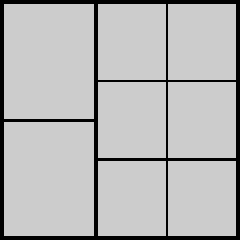
\includegraphics[width=\textwidth]{two_patch_basic}
		\caption{Simple non-conforming mesh}\label{fig:two_patch_biharmonic_problem_basic}
	\end{subfigure}
	\hfill
	\begin{subfigure}[t]{0.3\textwidth}
		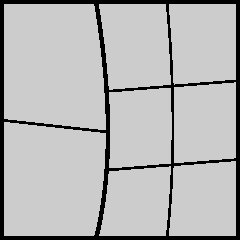
\includegraphics[width=\textwidth]{two_patch_distorted}
		\caption{Distorted non-conforming mesh}\label{fig:two_patch_biharmonic_problem_distorted}
	\end{subfigure}
	\hfill
	\begin{subfigure}[t]{0.3\textwidth}
		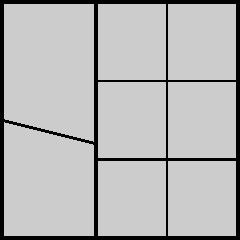
\includegraphics[width=\textwidth]{two_patch_nonmatch}
		\caption{non-conforming mesh with mismatched parameterizations}\label{fig:two_patch_biharmonic_problem_nonmatch}
	\end{subfigure}\\
	\begin{subfigure}[t]{0.35\textwidth}
		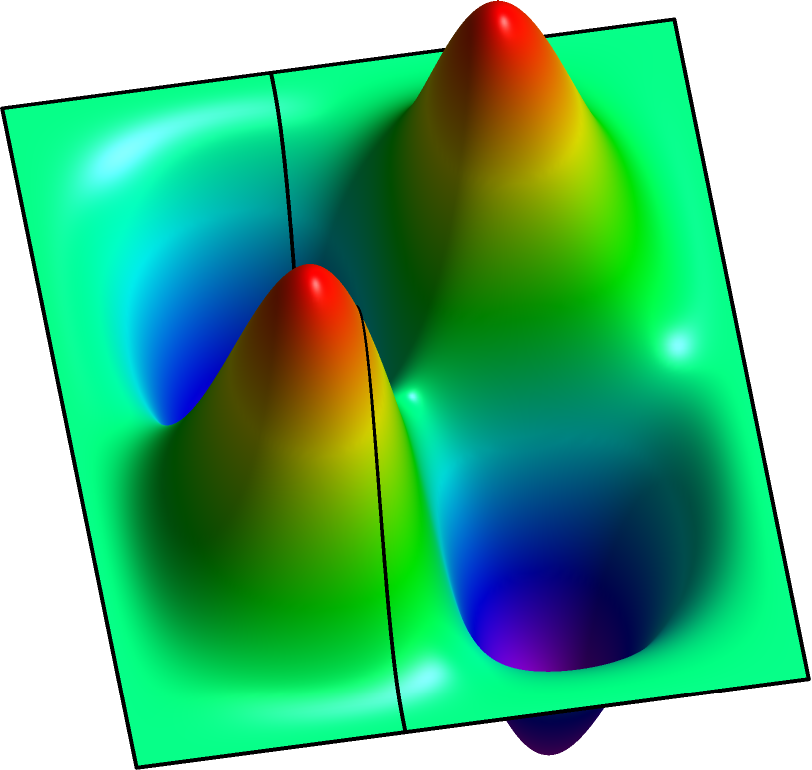
\includegraphics[width=\textwidth]{two_patches_solution-plot}

		\caption{The manufactured solution\vspace{3mm}}\label{fig:two_patch_biharmonic_problem_solution-plot}
	\end{subfigure}
	\caption{The discretizations of the domain $\Omega$ ((a) - (c)) and the manufactured solution (d) with the property $u=\frac{\partial{u}}{\partial{\mathbf{n}}}=0$ on $\partial{\Omega}$ for the problem in Section~\ref{sec:two_patch}.}\label{fig:two_patch_biharmonic_problem}
\end{figure}

\begin{figure}[ht]
	\centering
	\begin{subfigure}[b]{0.45\textwidth}
		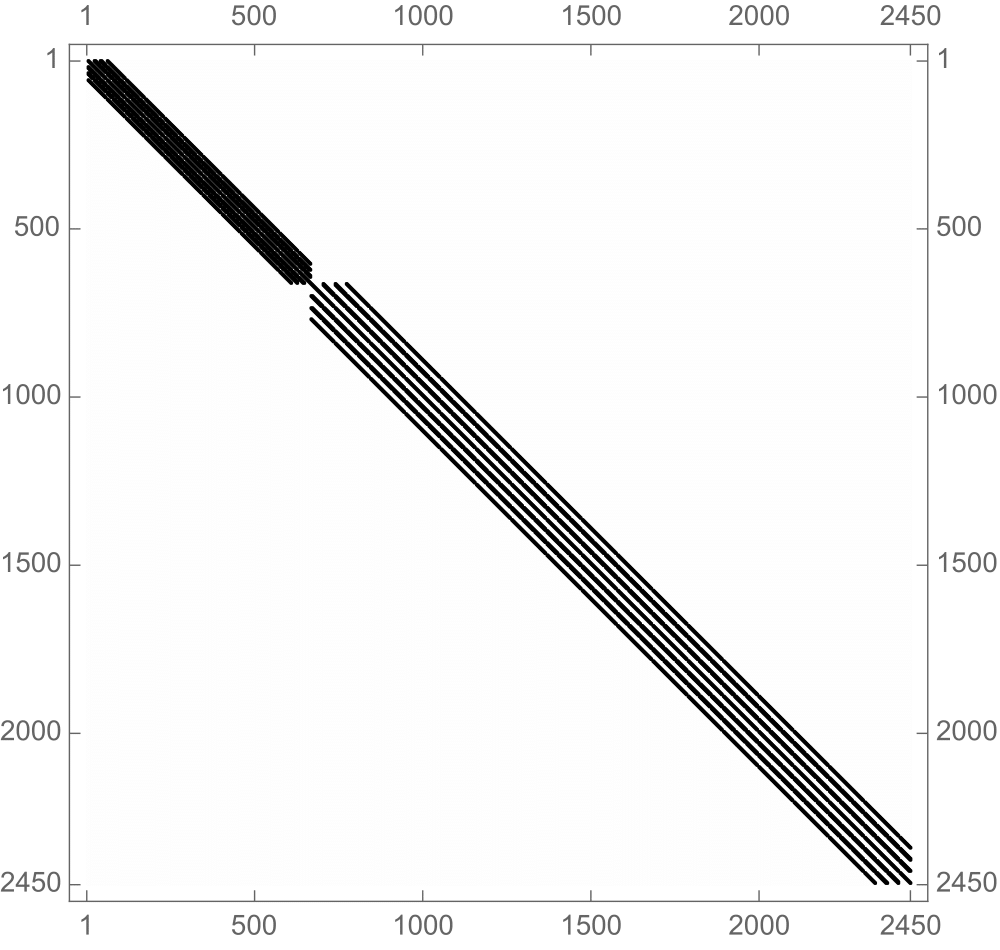
\includegraphics[width=\textwidth]{sp}
		\caption{}
	\end{subfigure}
	\begin{subfigure}[b]{0.45\textwidth}
		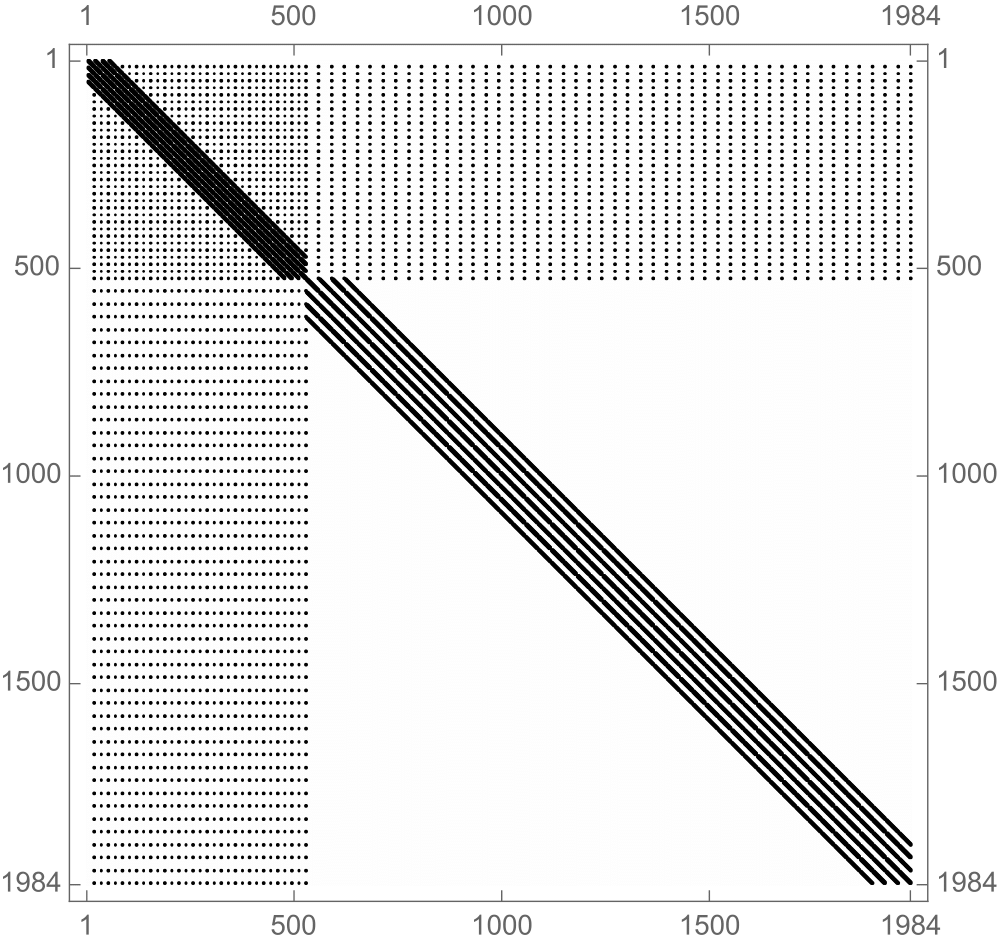
\includegraphics[width=\textwidth]{stand_sp}
		\caption{}
	\end{subfigure}
	\begin{subfigure}[b]{0.45\textwidth}
		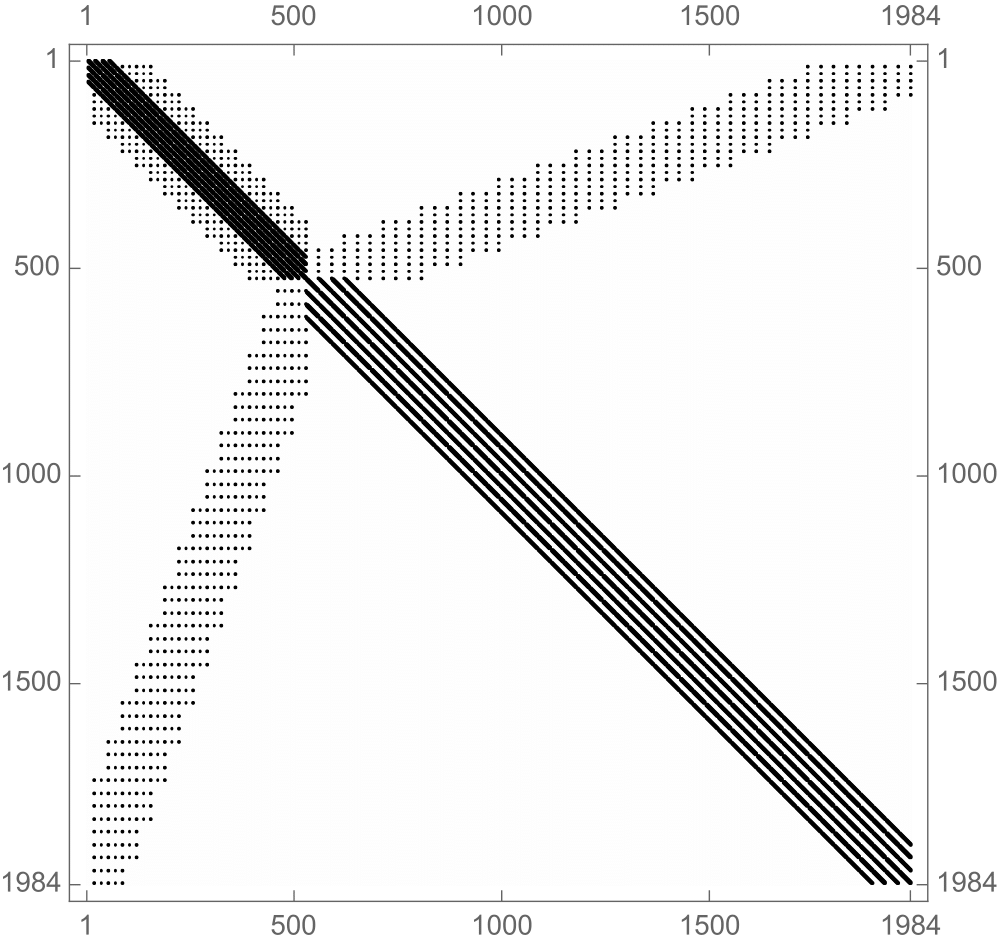
\includegraphics[width=\textwidth]{dual_sp}
		\caption{}
	\end{subfigure}
	\caption{Stiffness matrix sparsity patterns for (a) the uncoupled linear system, (b) the coupled linear system using the global dual basis, and (c) the coupled linear system using the \Bezier dual basis for the problem in Section~\ref{sec:two_patch}. The stiffness matrices are computed from the two-patch domain in Figure~\ref{fig:two_patch_biharmonic_problem_basic} after $4$ levels of refinement.}\label{fig:sparsity_pattern}
\end{figure}

The sparsity patterns for the stiffness matrices corresponding to the uncoupled problem, the coupled problem using the global dual basis, and the coupled problem using the \Bezier dual basis are shown in Figure~\ref{fig:sparsity_pattern}. Note that the matrix constructed using the global dual basis is denser than the matrix constructed using the \Bezier dual basis.\par

We conduct convergence studies for $p=2,3,4,5$ in both the $L^2$ and $H^2_*$ norms for the mesh shown in Figure~\ref{fig:two_patch_biharmonic_problem_basic}. The results are shown in Figure~\ref{fig:two_patc_biharmonic_convergence_basic}. Notice that despite the poor approximability of the \Bezier dual basis it performs surprisingly well in practice. As can be seen, both the global and B\'ezier dual basis obtain optimal convergence rates in both norms for all polynomial degrees. In fact, the convergence plots are almost identical between the global and \Bezier dual basis. The influence of the consistency error of the \Bezier dual basis cannot be observed for all tested polynomial degrees. We conjecture that for biharmonic problems, the coefficient $c_b$ in~\eqref{eq:consistency_error} is so small that the contribution of the consistency error in the finite element approximation is negligible.\par

\begin{figure}[ht]
	\centering
	\begin{subfigure}[b]{0.47\textwidth}
		\includestandalone[scale=.9]{two_patch_biharmonic_basic}
	\end{subfigure}
	\hfill
	\begin{subfigure}[b]{0.47\textwidth}
		\includestandalone[scale=.9]{two_patch_biharmonic_basic_H2}
	\end{subfigure}
	\caption{Convergence plots for the mesh shown in Figure~\ref{fig:two_patch_biharmonic_problem_basic}. Left: error measured in the $L^2$ norm. Right: error measured in the $H^2_*$ norm.}\label{fig:two_patc_biharmonic_convergence_basic}
\end{figure}

To study the performance of the proposed method in the presence of mesh distortion and mismatched parameterizations, we consider the meshes shown in Figure~\ref{fig:two_patch_biharmonic_problem_distorted} and~\ref{fig:two_patch_biharmonic_problem_nonmatch}. For the distorted mesh, shown in Figure~\ref{fig:two_patch_biharmonic_problem_distorted}, the proposed method with both global and B\'ezier dual basis functions perform similarly with optimal convergence rates being achieved in all cases as shown in Figure~\ref{fig:two_patc_biharmonic_convergence_distorted}.

For the mesh with mismatched parameterizations, shown in Figure~\ref{fig:two_patch_biharmonic_problem_nonmatch}, the convergence behavior of the B\'ezier dual basis, though optimal, deterioriates relative to the global dual basis as shown in Figure~\ref{fig:two_patc_biharmonic_convergence_nonmatch}. This indicates that the B\'ezier dual basis is more sensitive to mesh distortion than the global dual basis. Interestingly, as the mesh is refined, the results obtained using the $5^{th}$ order global dual basis become sub-optimal. We speculate that this is caused by an \textit{inf-sup} instability in this specific problem.

For the degree mismatched case shown in Figure~\ref{fig:two_patch_biharmonic_problem_basic}, the convergence rates are between $p_\text{left}+1$ and $p_\text{left}+2$ in the $L^2$ norm, and between $p_\text{left}-1$ and $p_\text{left}$ in the $H^2_*$ norm as expected for all cases and shown in Figure~\ref{fig:two_patc_biharmonic_convergence_diff_degree}. \par

\begin{figure}[ht]
	\centering
	\begin{subfigure}[b]{0.47\textwidth}
		\includestandalone[scale=.9]{two_patch_biharmonic_distorted}
	\end{subfigure}
	\hfill
	\begin{subfigure}[b]{0.47\textwidth}
		\includestandalone[scale=.9]{two_patch_biharmonic_distorted_H2}
	\end{subfigure}
	\caption{Convergence plots for the mesh shown in Figure~\ref{fig:two_patch_biharmonic_problem_distorted}. Left: error measured in the $L^2$ norm. Right: error measured in the $H^2_*$ norm.}\label{fig:two_patc_biharmonic_convergence_distorted}
\end{figure}

\begin{figure}[ht]
	\centering
	\begin{subfigure}[b]{0.47\textwidth}
		\includestandalone[scale=.9]{two_patch_biharmonic_nonmatch}
	\end{subfigure}
	\hfill
	\begin{subfigure}[b]{0.47\textwidth}
		\includestandalone[scale=.9]{two_patch_biharmonic_nonmatch_H2}
	\end{subfigure}
	\caption{Convergence plots for the mesh shown in Figure~\ref{fig:two_patch_biharmonic_problem_nonmatch}. Left: error measured in the $L^2$ norm. Right: error measured in the $H^2_*$ norm.}\label{fig:two_patc_biharmonic_convergence_nonmatch}
\end{figure}

\begin{figure}[ht]
	\centering
	\begin{subfigure}[b]{0.47\textwidth}
		\includestandalone[scale=.9]{two_patch_biharmonic_diff_degree}
	\end{subfigure}
	\hfill
	\begin{subfigure}[b]{0.47\textwidth}
		\includestandalone[scale=.9]{two_patch_biharmonic_diff_degree_H2}
	\end{subfigure}
	\caption{Convergence plots for the mesh shown in Figure~\ref{fig:two_patch_biharmonic_problem_basic} with mismatched degrees. Left: error measured in the $L^2$ norm. Right: error measured in the $H^2_*$ norm.}\label{fig:two_patc_biharmonic_convergence_diff_degree}
\end{figure}

Although a functional analysis of the contribution of the consistency error in the finite element approximation error is beyond the scope of this paper and postponed for future work, here we study the influence of the consistency error in a numerical manner. Since the finite element error is composed of the approximation error and the consistency error, the effect of the consistency error can be demonstrated by a comparison between the finite element error and the approximation error. The approximation error is the best $H^2_*$ approximation of $u$ in the discretized weak $C^1$ space $\mathcal{K}_b^h$, which is given as: find $u\in\mathcal{K}_b^h$ such that
\begin{equation}
	\langle{v^h,u^h}\rangle_{H^2_*}= \langle{v^h,u}\rangle_{H^2_*}\quad\quad\forall{v^h\in\mathcal{K}_b^h}.
\end{equation}

Plots of the approximation error for the proposed method for the meshes shown in Figure~\ref{fig:two_patch_biharmonic_problem} are shown in Figure~\ref{fig:two_patch_best_approximation}. As can be seen, the convergence plots of the approximation error are identical to those of the finite element error in the $H^2_*$ norm. The approximation errors for all cases are no more than $1\%$ smaller than their finite element counterparts, which confirms our conjecture that the contribution of the best approximation error for the Lagrange multipliers (the consistency error) are negligible for the problems we tested. In addition, the approximation error plots for the global dual basis also demonstrate wavy and less asymptotic behavior. For the $p=5$ mismatched non-conforming mesh case it also suffers from reduced convergence rates, which confirms that the main cause of this phenomena in the finite element approximation is due to the \textit{inf-sup} instability.\par


\begin{figure}[ht]
	\captionsetup[subfigure]{labelformat=empty, font = footnotesize, justification=centering}
	\centering
	\begin{subfigure}[b]{0.47\textwidth}
		\includestandalone[scale=.9]{two_patch_biharmonic_basic_H2}
		\caption{Simple non-conforming mesh}
		\vspace*{3mm}
	\end{subfigure}
	\hfill
	\begin{subfigure}[b]{0.47\textwidth}
		\includestandalone[scale=.9]{two_patch_biharmonic_distorted_H2}
		\caption{Distorted non-conforming mesh}
		\vspace*{3mm}
	\end{subfigure}
	%
	\begin{subfigure}[b]{0.47\textwidth}
		\includestandalone[scale=.9]{two_patch_biharmonic_nonmatch_H2}
		\caption{Mismatched non-conforming mesh}
	\end{subfigure}
	\hfill
	\begin{subfigure}[b]{0.47\textwidth}
		\includestandalone[scale=.9]{two_patch_biharmonic_diff_degree_H2}
		\caption{Degree mismatched non-conforming mesh}
	\end{subfigure}
	\caption{Convergence plots of the approximation error for the two-patch coupling problem shown in Figure~\ref{fig:two_patch_biharmonic_problem} and described in Section~\ref{sec:two_patch}.}\label{fig:two_patch_best_approximation}
\end{figure}


\subsection{The biharmonic problem on multi-patch domains}
\subsubsection{The biharmonic problem on a three-patch domain}\label{sec:three-patch}
We now examine the proposed method for multi-patch coupling. We first solve a biharmonic problem with the manufactured solution
\begin{equation}
	u(x,y)=sin(2\pi{x})sin(2\pi{y})\left({y(3x-y)(3x+2y-9)}\right)^2,
\end{equation}
on the triangular domain decomposed into three patches as shown in Figure~\ref{fig:three_patch_biharmonic_problem}. Both multi-patch treatments are tested in this problem.

\begin{figure}[ht]
	\centering
	\begin{subfigure}[b]{0.33\textwidth}
		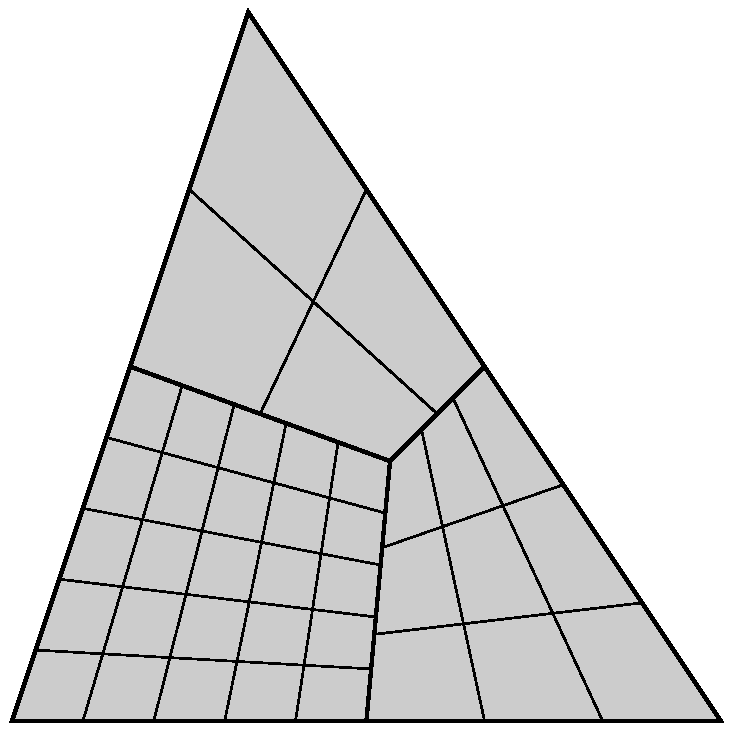
\includegraphics[width=\textwidth]{three_patch_basic}
		\caption{Non-conforming mesh}
	\end{subfigure}
	\begin{subfigure}[b]{0.41\textwidth}
		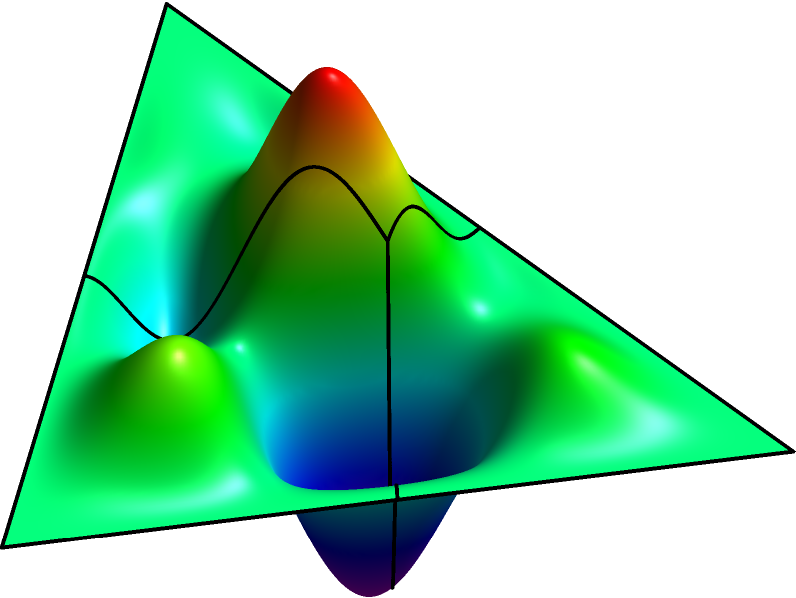
\includegraphics[width=\textwidth]{three_patches_solution-plot}
		\caption{The manufactured solution}
	\end{subfigure}
	\caption{The three-patch domain and the manufactured solution for the problem in Section~\ref{sec:three-patch}.}\label{fig:three_patch_biharmonic_problem}
\end{figure}

The results are shown in Figure.~\ref{fig:three_patc_biharmonic_convergence}. As can be seen, the MG method yields optimal convergence rates in both measures for all tested polynomial orders. The MB method, on the other hand, yields $\mathcal{O}(h)$ convergence in $H^2_*$ norm and $\mathcal{O}(h^2)$ convergence in $L^2$ norm. The poor performance of the MB method is due to the consistency error, which can be verified by the optimal convergence rates in the approximation error (see Figure~\ref{fig:three_patch_approximation}). Moreover, for $p=3,4,5$, the finite element error increases as the polynomial order increases, which is consistent with the approximation power of the \Bezier dual basis (see Figure~\ref{fig:l_2_error}). Nevertheless, despite the sub-optimal convergence for certain circumstances, the MB method still converges asymptotically for all tested cases. The OG method yields optimal results for all tested polynomial orders except $p=5$. The sub-optimal rate for $p=5$ in both the $L^2$ and $H^2_*$ norms is due to the approximation error (see Figure~\ref{fig:three_patch_approximation}). Although the consistency error still influences the finite element approximation of the OB method, the error level at which the consistency error dominates is much lower ($10^{4}$ times lower in the $L^2$ norm and $10^{3}$ times lower in the $H^2_*$ norm) than that of the MB method. As a result, for $p=2,3,4$, the results obtained from the OB method demonstrate optimal convergence with sub-optimal convergence only occurring at the finest mesh for $p=5$. The approximation error for both the MB and OB methods are optimal for all tested polynomial orders, which indicates the \textit{inf-sup} stability of the proposed method with the \Bezier dual basis.

\begin{figure}[ht]
	\centering
	\begin{subfigure}[b]{0.47\textwidth}
		\includestandalone[scale=.9]{three_patch_modify_biharmonic_basic}
	\end{subfigure}
	\hfill
	\begin{subfigure}[b]{0.47\textwidth}
		\includestandalone[scale=.9]{three_patch_modify_biharmonic_basic_H2}
	\end{subfigure}
	\begin{subfigure}[b]{0.47\textwidth}
		\includestandalone[scale=.9]{three_patch_biharmonic_basic}
	\end{subfigure}
	\hfill
	\begin{subfigure}[b]{0.47\textwidth}
		\includestandalone[scale=.9]{three_patch_biharmonic_basic_H2}
	\end{subfigure}
	\caption{Convergence plots for the three-patch problem in Section~\ref{sec:three-patch}. Left: error measured in $L^2$ norm. Right: error measured in $H^2_*$ norm.}\label{fig:three_patc_biharmonic_convergence}
\end{figure}


\begin{figure}[ht]
	\centering
	\begin{subfigure}[b]{0.47\textwidth}
		\includestandalone[scale=.9]{three_patch_modify_projection_basic_H2}
	\end{subfigure}
	\hfill
	\begin{subfigure}[b]{0.47\textwidth}
		\includestandalone[scale=.9]{three_patch_projection_basic_H2}
	\end{subfigure}
	\caption{Convergence plots of the approximation error for three-patch coupling in Section.~\ref{sec:three-patch}.}\label{fig:three_patch_approximation}
\end{figure}
\FloatBarrier

\subsubsection{The biharmonic problem on a five-patch domain}\label{sec:five-patch}

To further study the effect of in-domain vertices, we solve a biharmonic problem on a five-patch domain, as shown in Figure~\ref{fig:five_patch_biharmonic_problem}, with the manufactured solution
\begin{equation}
	u(x,y)=\sin(2\pi{x})^2\sin(2\pi{y})^2.
\end{equation}

\begin{figure}[ht]
	\centering
	\begin{subfigure}[b]{0.33\textwidth}
		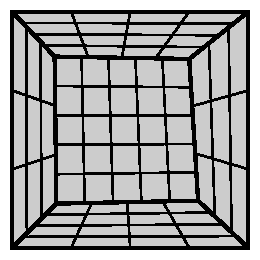
\includegraphics[width=\textwidth]{five_patch_basic}
		\caption{Non-conforming mesh}
	\end{subfigure}
	\begin{subfigure}[b]{0.34\textwidth}
		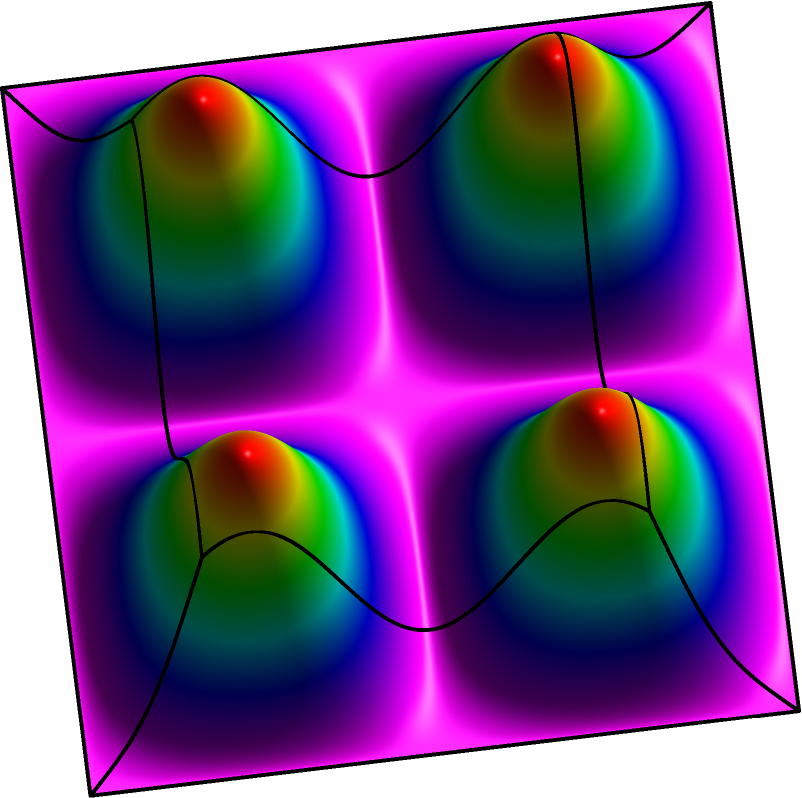
\includegraphics[width=\textwidth]{five_patch_solution-plot}
		\caption{The manufactured solution}
	\end{subfigure}
	\caption{The five-patch domain parameterization and the manufactured solution in Section~\ref{sec:five-patch}.}\label{fig:five_patch_biharmonic_problem}
\end{figure}

\begin{figure}[ht]
	\centering
	\begin{subfigure}[b]{0.47\textwidth}
		\includestandalone[scale=.9]{five_patch_modify_biharmonic_basic}
	\end{subfigure}
	\hfill
	\begin{subfigure}[b]{0.47\textwidth}
		\includestandalone[scale=.9]{five_patch_modify_biharmonic_basic_H2}
	\end{subfigure}

	\begin{subfigure}[b]{0.47\textwidth}
		\includestandalone[scale=.9]{five_patch_biharmonic_basic}
	\end{subfigure}
	\hfill
	\begin{subfigure}[b]{0.47\textwidth}
		\includestandalone[scale=.9]{five_patch_biharmonic_basic_H2}
	\end{subfigure}
	\caption{Convergence plots for the five-patch problem in Section~\ref{sec:three-patch}. Left: error measured in $L^2$ norm. Right: error measured in $H^2_*$ norm.}\label{fig:five_patc_biharmonic_convergence}
\end{figure}

The convergence behavior for all methods is shown in Figure~\ref{fig:five_patc_biharmonic_convergence}. The approximation error plots are shown in Figure~\ref{fig:five_patch_approximation}. The results are similar to that of the three-patch case. For the global dual basis, the MG method gives optimal convergence rates for both the $L^2$ and $H^2$ norms, while the OG method has an \textit{inf-sup} instability, which disrupts convergence rates for fine meshes. The OB method postpones the domination of the consistency error (i.e., postponed from $10^{-3}$ and $10^{-1}$ to $10^{-7}$ and $10^{-4}$ in the $L^2$ and $H^2$ norm, respectively) and significantly improves convergence rates.

\begin{figure}[ht]
	\centering
	\begin{subfigure}[b]{0.47\textwidth}
		\includestandalone[scale=.9]{five_patch_modify_projection_basic_H2}
	\end{subfigure}
	\hfill
	\begin{subfigure}[b]{0.47\textwidth}
		\includestandalone[scale=.9]{five_patch_projection_basic_H2}
	\end{subfigure}
	\caption{Convergence plots of the approximation error for five-patch coupling in Section.~\ref{sec:five-patch}.}\label{fig:five_patch_approximation}
\end{figure}
\FloatBarrier

\subsection{Transverse vibrations of an elastic membrane}\label{sec:eigenvalue}

We now study the OB method in the context of a $2^\text{nd}$-order eigenvalue problem. Of particular interest is the behavior of the highest frequencies in the system since they govern the critical timestep size in an explicit time-stepping scheme. In particular, we consider the transverse vibration of a square, elastic membrane on the domain $\left[{0,3}\right] \times \left[{0,3}\right]$ with the nonconforming discretization shown in Figure~\ref{fig:eigenvalue_mesh}. The natural frequencies and modes are governed by
\begin{equation}
	\left\{\begin{split}
		\nabla^2 u(x,y) +\omega^2 u(x,y) = 0, & \text{ in } \Omega,\\
		u(x, y) = 0 & \text{ on } \partial \Omega,
	\end{split}\right.
\end{equation}
where $\omega$ is the natural frequency. The exact natural frequencies are

\begin{equation}
	\omega_{mn} = \pi \sqrt{\left(\frac{m}{L}\right)^2+\left(\frac{n}{L}\right)^2},\quad\quad m,n = 1,2,3,\dots,
\end{equation}
where $L$ is the length of the boundary.\par

The highest computed eigenvalues for the OB method are given in Table~\ref{tab:eigenvalues}. As can be seen, the weak $C^1$ coupling dramatically reduces the highest eigenvalues for all tested cases. The effect becomes more significant as the polynomal degree is increased. For $p=5$, the highest eigenvalue obtained through weak $C^1$ coupling is $\frac{3}{5}$ of that obtained through weak $C^0$ coupling. The normalized discrete spectra for $p=5$ are shown in Figure~\ref{fig:spectra}. In this case, weak $C^1$ coupling improves the behavior of the entire spectra.

\begin{figure}[ht]
	\centering
	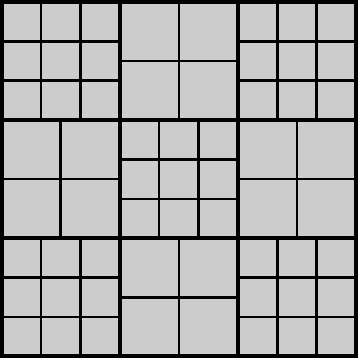
\includegraphics[width=.3\textwidth]{eigenvalue_mesh}
	\caption{The nine-patch domain parameterization for the eigenvalue problem in Section~\ref{sec:eigenvalue}.}\label{fig:eigenvalue_mesh}
\end{figure}

\begin{table}[!htbp]
	\centering
	\caption{The highest eigenvalues obtained by solving the eigenvalue problem for the square domain (see Figure~\ref{fig:eigenvalue_mesh})}
	\begin{tabular*}{\textwidth}{c @{\extracolsep{\fill}} SSSSSSSS}
		\toprule
		Refine &  \multicolumn{2}{c}{OB-$Q_2$} & \multicolumn{2}{c}{OB-$Q_3$} & \multicolumn{2}{c}{OB-$Q_4$} & \multicolumn{2}{c}{OB-$Q_5$}\\\cmidrule(lr{.5em}){2-3}\cmidrule(lr{.5em}){4-5}\cmidrule(lr{.5em}){6-7}\cmidrule(lr{.5em}){8-9}
		{} & \multicolumn{1}{c}{$C^0$} & \multicolumn{1}{c}{$C^1$} & \multicolumn{1}{c}{$C^0$} & \multicolumn{1}{c}{$C^1$} & \multicolumn{1}{c}{$C^0$} & \multicolumn{1}{c}{$C^1$} & \multicolumn{1}{c}{$C^0$} & \multicolumn{1}{c}{$C^1$}\\
		\midrule
		0   &  16.12  & 11.47  & 24.76  & 16.36 & 35.38  & 22.56  & 48.48  & 29.43\\
		1   &  20.97  & 17.41  & 29.39  & 20.86 & 41.41  & 26.91  & 54.60  & 34.18\\
		2   &  31.30  & 28.04  & 43.60  & 30.39 & 60.49  & 37.35  & 79.57  & 46.82\\
		3   &  54.04  & 52.61  & 78.60  & 51.09 & 108.47 & 61.75  & \cellcolor{hred!30}141.44 & \cellcolor{hred!30}81.53\\
		\bottomrule
	\end{tabular*}
	\label{tab:eigenvalues}
\end{table}

\begin{figure}[ht]
	\centering
	\includestandalone[scale=1.2]{spectrum}
	\caption{Normalized discrete spectra using $p=5$. Results are obtained after three uniform refinements.}\label{fig:spectra}
\end{figure}
\FloatBarrier

\section{Conclusion}\label{sec:conclusion}

In this paper, we present a dual mortar formulation for the biharmonic problem and investigate its properties analytically and numerically. With the help of the dual mortar suitable $C^1$ constraint, the biorthogonality between the dual basis functions and the corresponding primal spline basis functions can be extended to the discretized $C^1$ constraint matrix. Hence, the condensed stiffness matrix can be formed efficiently without the need to solve linear systems associated with each intersection. Furthermore, the condensed stifness matrix remains sparse if the dual basis functions are compactly supported, which is the case for the \Bezier dual basis.\par

Due to the presence of in-domain vertices, some control points may serve as both slave and master. To overcome this we propose two solutions. The first method localizes the constraints to the neighborhood of each vertex and solves for the null space of a localized linear system. The second method reduces the number of constraints at each vertex by reducing the number of degrees of freedom of the dual basis. For both cases, when the \Bezier dual basis is used, the resulting linear systems are sparse. A suite of numerical experiments demonstrate the effectiveness of the proposed approach. \par
% \chapter{The enriched B\'ezier dual basis}
\label{chp:chapter4}
\graphicspath{{figures/}{figures/chapter4/}}
\pgfplotsset{
    table/search path={{figures/chapter4/data},{data}},
}
\externaldocument[iii-]{exampleFiles/chapter3}
\externaldocument[ii-]{exampleFiles/chapter2}

In the previous chapter, we studied the approximation power of the \Bezier dual basis and the cause of its sub-optimality is the lack of polynomial reproduction. The sub-optimality of the \Bezier dual basis deteriorate the finite element approximation when is used as the discretization of Lagrange multiplier. The development of dual basis functions that are able to reproduce higher order polynomials while maintain compact support is crucial for the implementation of the dual mortar formulation in the previous chapter.\par

Dual functional of splines was first introduced by de Boor and Fix~\cite{de1973spline} to develop a quasi-interpolation operator for splines. Later on, de Boor presented dual basis functions in~\cite{de1975local}. Thomas et al.~\cite{thomas2015bezier} introduced the \Bezier projection operator as an efficient replacement of global $L^2$ projection. The dual basis induced by \Bezier projection operator has been utlized in~\cite{MIAO2018273,zou2018isogeometric} for alleviating locking and patch coupling, correspondingly. In the finite element framework, the construction of dual basis function with optimal appxoimation power was first presented in~\cite{oswald2001polynomial}. In~\cite{lamichhane2002higher}, Lamichhane and Wohlmuth introduced locally supported and continuous dual basis functions for quadratic finite elements. Later on, Lamichhane and Wohlmuth developed a group of dual basis that have the same support as the nodal finite element basis and possess adequate approximation power. Very recently, Wunderlich et al.~\cite{wunderlich2019biorthogonal} extend the formulation in~\cite{oswald2001polynomial} to the context of isogeometric analysis.\par

However, the construction algorithm in~\cite{oswald2001polynomial} calls the assembly routine twice--the first call is to construct dual basis with minimal support while the enrichment of dual basis is finished in the second call, which is inconvenient from the implementation perspective. Moreover, the condition numbers of a series of linear problems solved in~\cite{oswald2001polynomial} grow at the rate $p$, which may not be an issue for lower order basis. However, this may pollute results from higher order basis on large scale problems. \par

Based the formulation given in~\cite{oswald2001polynomial}, we propose a quadrature-free algorithm to efficiently construct enriched dual basis functions that reproduce polynomial up to a given degree. The linear systems solved in our algorithm is independent of the mesh size. Hence, there is no needs to take care of the conditioning. In addition, we utilize the enriched dual basis in the dual mortaring of $4^\text{th}$ order problems. \par

\section{Dual basis functions}

\subsection{Bernstein dual basis functions}
For a primal Bernstein basis $\mathbf{B}$, a dual basis $\hat{\mathbf{B}}$ can be formulated simply using the inverse Gramian as
\begin{equation}
	\hat{\mathbf{B}} = \mathbf{G}^{-1}\mathbf{B}.\label{eq:global_dual}
\end{equation}

\begin{figure}
    \centering
    \begin{subfigure}{.48\linewidth}
        \center
        \includestandalone[scale = .8]{bezier}
    \end{subfigure}
    \begin{subfigure}{.48\linewidth}
        \center
        \includestandalone[scale = .8]{bezier_dual}
    \end{subfigure}
	\caption{Piecewise \Bezier basis (left) and the corresponding dual basis (right) of degree $p=2$ defined by the knot vector $\left\{0,0,0,1/3,2/3,1,1,1\right\}$. Note that each dual basis has the same support as the corresponding primal basis function.}
	\label{fig:bezier_and_its_dual}
\end{figure}
A graphical depiction of Bernstein basis functions and the corresponding dual basis functions is shown in Figure~\ref{fig:bezier_and_its_dual}. The Bernstein dual basis $\hat{\mathbf{B}}$ has the following properties:
\begin{itemize}
	\item{\textbf{Local support.}} The Bernstein dual basis is locally supported and each dual basis has the same support as the corresponding primal basis function, i.e., $\supp{\hat{B}_i}=\supp{{B}_i}$.
	\item{\textbf{Polynomial completeness.}} The space spanned by the dual basis is the same as the space spanned by the primal Bernstein basis, i.e., $\spn\{\hat{\mathbf{B}}\}=\spn\{\mathbf{B}\}=\mathcal{X}$.
\end{itemize}

\subsection{B-spline dual basis functions}
For a primal B-spline basis $\mathbf{N}$, a dual basis $\hat{\mathbf{N}}$ can be formulated as
\begin{equation}
	\langle\hat{N}_i,N_j\rangle_\Omega:=\int_\Omega\hat{N}_iN_jd\Omega=\delta_{ij}.
\end{equation}
We denote the spans of ${\mathbf{N}}$ and $\hat{\mathbf{N}}$ by $\mathcal{N},\hat{\mathcal{N}}\subset\mathcal{X}$, respectively. We can also introduce a pair of quasi-interpolation operators
\begin{equation}
	\quasii{N}u = \sum_i\langle{\hat{N}_i,u}\rangle_\Omega{N}_i\text{, and }\quasiid{N}u = \sum_i\langle{{N}_i,u}\rangle_\Omega\hat{N}_i.\label{eq:quasi-interpolation-operators}
\end{equation}
\begin{remark}
	Both $\quasii{N}$ and $\quasiid{N}$ are projection operators, i.e., for all $u\in\mathcal{N}$, $v\in\hat{\mathcal{N}}$, $\quasii{N}u=u$ and $\quasiid{N}v=v$.
\end{remark}

The construction of a B-spline dual basis with the same properties as the Bernstein dual basis, i.e., local support and polynomial completeness, is challenging. A globally supported B-spline dual basis with polynomial completeness can be constructed using an inverse Gramian (see Equation~\eqref{eq:global_dual}). On the other hand, a locally supported B-spline dual basis which does not have polynomial completeness can be constructed using the \Bezier extraction procedure as follows:
\begin{lemma}
	$\{\hat{\mathbf{N}}\}\in\mathcal{X}$ is dual to ${\mathbf{N}}$ if and only if
	\begin{equation}
		\hat{\mathbf{N}} = \mathbf{W}^T\mathbf{R}^T\mathbf{G}^{-1}\mathbf{B}=\mathbf{W}^T\mathbf{R}^T\hat{\mathbf{B}},\label{eq:dual_basis_form}
	\end{equation}
	where the weighted assembly matrix $\mathbf{W}^T$ is a pseudo-inverse of $\mathbf{A}$, i.e., $\mathbf{W}^T\mathbf{A} = \mathbf{I}$.
\end{lemma}
\begin{proof}
	Given a basis vector in form~\eqref{eq:dual_basis_form}, its inner product with the spline basis vector is given by
	\begin{equation}
		\langle\hat{\mathbf{N}},\mathbf{N}^T\rangle_\Omega = \mathbf{W}^T\mathbf{R}^T\langle\hat{\mathbf{B}},\mathbf{B}^T\rangle_\Omega\mathbf{C}^T\mathbf{A}=\mathbf{I}.
	\end{equation}
	On the other hand, if we assume that $\{\hat{\mathbf{N}}\}\in\mathcal{X}$ is dual to ${\mathbf{N}}$, then since $\hat{N}_i=\quasii{X}\hat{N}_i=\sum_j\langle \hat{B}_j, \hat{N}_i\rangle \hat{B}_j$, we can rewrite the basis vector $\hat{\mathbf{N}}$ in terms of $\hat{\mathbf{B}}$ as
	\begin{equation}
		\hat{\mathbf{N}} = \tilde{\mathbf{W}}^T\hat{\mathbf{B}}\text{, with } \tilde{W}_{i,j} = \langle{\hat{B}_i,\hat{N}_j}\rangle_\Omega.
	\end{equation}
	Hence, one can rewrite $\hat{\mathbf{N}}$ in form~\eqref{eq:dual_basis_form}, with $\mathbf{W}=\mathbf{C}\tilde{\mathbf{W}}$.
\end{proof}
We can now see that the construction of a locally supported dual basis can be simplified to finding a set of banded vectors $\{\mathbf{W}_i\}_{i=0}^{n_N-1}$ such that
\begin{equation}
	\mathbf{W}_i\cdot\mathbf{A}_j=\delta_{ij}.\label{eq:biorthonormal}
\end{equation}

\begin{remark}
	Various dual basis functions for splines have been constructed in recent years. Using the fact that the assembly operator for splines is orthogonal to itself , i.e. $\mathbf{A}_i\mathbf{A}_j = c_j\delta_{ij}$, Seitz et al.~\cite{seitz2016isogeometric} utilized $\mathbf{A}$ as the assembly matrix in the construction of dual basis functions, the resulted dual basis functions satisfy the biorthogonal relation $\langle\hat{N}_i,N_j\rangle_\Omega=c_j\delta_{ij}$. In~\cite{thomas2015bezier}, Thomas et al. introduced a weighting scheme in constructing the assembly matrix $\mathbf{W}$ for dual basis functions. The weight of each dual basis functions in each elements are based on the area proportions of their primal counterparts. The resulted $\mathbf{W}$ satisfies the biorthonormal relation~\eqref{eq:biorthonormal} and the constructed dual basis has excellent performance when used as the quasi-interpolation operator $\quasii{N}$.
\end{remark}

\begin{remark}\label{rm:dual_qi_sub_optimal}
	Note that, in most cases, a locally constructed quasi-interpolation operator $\quasii{N}$ possesses optimal approximation power. However, without special care, the corresponding locally constructed dual quasi-interpolation operator $\quasiid{N}$ possesses sub-optimal approximation power. In fact, for any degree it usually provides an approximation accuracy of only $\mathcal{O}(h)$. This is due to the fact that $\quasiid{N}$ lacks polynomial completeness.
\end{remark}

\section{The approximation power of dual bases}\label{sec:approximation}

In addition to the application of the dual basis as a local functional for the quasi-interpolation operator $\quasii{N}$, the dual basis is also widely used to solve constrained finite element problems. The advantage of using a dual basis as the Lagrange multiplier is that the degrees of freedom associated with the multiplier can be locally condensed out leading to a sparse, positive-definite linear system.

However, the best finite element approximation of the Lagrange multiplier method is governed by the approximation power of the Lagrange multiplier. The approximation power of a conventional dual basis does not improve as the polynomial degree is increased. In this section, we discuss the theoretical requirements that a dual basis must satisfy to improve the approximation power to a given order. \par

We first state the approximation properties of a polynomial space $\mathcal{P}$, the proof of which can be found in~\cite{brenner_mathematical_2007}.
\begin{lemma}\label{lm:bramble-hilbert}
	(Bramble-Hilbert) Let $\Omega$ be star-shaped and $Q^qu$ be the Taylor polynomial of order $q$ of $u\in{H}^{q+1}(\Omega)$, then
	\begin{equation}
		\vert{u-Q^qu}\vert_{H^k(\Omega)}\leq{}C_{bh}h^{q+1-k}\vert{u}\vert_{H^{q+1}(\Omega)},\quad{}k=\left\{0,1,\dots,q+1\right\},
	\end{equation}
	where $h$ is the diameter of $\Omega$.
\end{lemma}

\begin{assumption}\label{aspt:global_polynomial_reproduction}
	(global idempotence) The dual quasi-interpolation operator $\quasiid{N}$ preserves polynomials of degree $q$ on the entire domain, i.e.,
	\begin{equation}
		\quasiid{N}p=p,\quad\forall{}p\in\mathcal{P}^q{(\Omega)}.
	\end{equation}
\end{assumption}

\begin{assumption}\label{aspt:local_support}
	(local support) Each dual basis function $\hat{N}_i$ is supported by at most $m$ connected elements and $\supp{{N}_i}\subset\supp{\hat{N}_i}$.
\end{assumption}

From Assumption~\ref{aspt:global_polynomial_reproduction} and Assumption~\ref{aspt:local_support}, we have the following result:
\begin{lemma}\label{lemma:local_polynomial_reproduction}
	(local idempotence) For each element $\Omega_e\subset\Omega$, there is an extension element $\hat{\Omega}_e$ comprised of a fixed number of connected elements such that
	\begin{equation}
		\left(\quasiid{N}p\right)\vert_{\Omega_e}=p,\quad\forall{}p\in\mathcal{P}^q{(\hat{\Omega}_e)}.
	\end{equation}
	\begin{proof}
		We define
		\begin{equation}
			\hat{\Omega}_e=
			\begin{cases}
				\bigcup_{i=0}^{e+m-1}\Omega_i,\quad{e-m+1<0}         \\
				\bigcup_{i=e-m+1}^{n_e-1}\Omega_i,\quad{e+m-1>n_e-1} \\
				\bigcup_{i=e-m+1}^{e+m-1}\Omega_i,\quad\text{otherwise},
			\end{cases}
		\end{equation}
		where $n_e$ is the number of elements in $\Omega$. Since each $\hat{N}_i$ is supported by at most $m$ connected elements, if $\Omega_e\subset\supp{\hat{N}_i}$, then $\supp{\hat{N}_i}\subset\hat{\Omega}_e$ and the evaluation $\langle{N_i,p}\rangle$ in~\eqref{eq:quasi-interpolation-operators} can be done in $\hat{\Omega}_e$, owing to $\supp{{N}_i}\subset\supp{\hat{N}_i}$. Hence, local polynomial preservation can be obtained from the global idempotence for polynomials.
	\end{proof}
\end{lemma}

\begin{assumption}\label{aspt:local_stability}
	(local stability) The restriction of the dual quasi-interpolation operator $\quasiid{N}$ on $\Omega_e$ is bounded, i.e.,
	\begin{equation}
		\|\quasiid{N}u\|_{H^k(\Omega_e)}\leq{}C_{st}\|u\|_{H^k(\hat{\Omega}_e)}.
	\end{equation}
\end{assumption}

Using the Bramble-Hilbert lemma, local idempotence, and local stability, we can state the convergence behavior of the dual quasi-interpolation operator $\quasiid{N}$.

\begin{theorem}
	Let $k$ and $m$ be integer indices with $0\leq{k}\leq{m}\leq{q+1}$ and $u\in{}H^m(\hat{\Omega}_e)$. Then for $0\leq{}k\leq{}m$, we have
	\begin{equation}
		\|{u-\quasiid{N}u}\|_{H^k(\Omega_e)}\leq{}C_{}h^{m-k}\|{u}\|_{H^m(\hat{\Omega}_e)}
	\end{equation}
	\begin{proof}
		$\forall{}p\in\mathcal{P}^q(\hat{\Omega}_e)$, we have
		\begin{align}
			\begin{split}
				\|{u-\quasiid{N}u}\|_{H^k(\Omega_e)}&\leq{}\|{u-p}\|_{H^k(\Omega_e)}+\|{p-\quasiid{N}u}\|_{H^k(\Omega_e)}\\
				&=\|{u-p}\|_{H^k(\Omega_e)}+\|{\quasiid{N}(p-u)}\|_{H^k(\Omega_e)}\\
				&\leq{}(1+C_{st})\|{u-p}\|_{H^k(\hat{\Omega}_e)},
			\end{split}
		\end{align}
		by choosing $p=Q^qu$, we have
		\begin{equation}
			\|{u-\quasiid{N}u}\|_{H^k(\Omega_e)}\leq{}(1+C_{st})\|{u-Q^qu}\|_{H^k(\hat{\Omega}_e)}\leq{}C_{bh}(1+C_{st})h^{m-k}\|{u}\|_{H^m(\hat{\Omega}_e)}.
		\end{equation}
	\end{proof}
\end{theorem}
Hence, in order for the quasi-interpolation operator $\quasiid{N}$ to converge at a given rate $q+1$, $\quasiid{N}$ must preserve polynomials on the entire domain up to degree $q$. In addition, the local support and local stability requirements must be satisfied. In the next section, we will construct a dual basis that satisfies Assumption~\ref{aspt:global_polynomial_reproduction} and explain how the construction procedure ensures the satisfaction of Assumption~\ref{aspt:local_support} and Assumption~\ref{aspt:local_stability}.

\section{Embedding polynomials into the dual basis function space}\label{sec:algorithm}

We now describe how to construct a set of enriched dual basis functions which will endow $\quasiid{N}$ with polynomial reproduction up to a given degree. The construction is a two-step procedure:
\begin{enumerate}
\item For a given assembly matrix $\mathbf{A}$, we find a set of sparse vectors $\{\mathbf{W}^\text{ini}_i\}_{i=0}^{n_N-1}$ such that $\mathbf{W}^\text{ini}_i\cdot\mathbf{A}_j=\delta_{ij}$. Its matrix form $\mathbf{W}^\text{ini}$ is considered to be the initial guess for the assembly matrix $\mathbf{W}$ of the desired dual basis.
  \item The vectors $\mathbf{W}^\text{ini}$ are then modified by vectors $\{\mathbf{W}^\text{mod}_i\}_{i=0}^{n_N-1}$ which come from the null space of $\spn\left\{\mathbf{A}_i\right\}_{i=0}^{n_N-1}$ until the required property is fulfilled. Note that such a modification will maintain the biorthogonal relation between $\{\mathbf{W}_i\}_{i=0}^{n_N-1}$ and $\{\mathbf{A}_i\}_{i=0}^{n_N-1}$ where
\begin{equation}
	\mathbf{W}_i=\mathbf{W}^\text{ini}_i+\mathbf{W}^\text{mod}_i.
\end{equation}
\end{enumerate}


\subsection{An orthonormal basis for the space $\mathbb{R}^{n_B}$}

To facilitate the construction of the enriched dual basis, we build a set of orthonormal vectors which form a basis for $\mathbb{R}^{n_B}$. Each orthonormal vector will have minimal support, where the support of a vector is taken to be the distance between the first and last nonzero entry. From the properties of the assembly operator $\mathbf{A}$ in Chapter~\ref{chp:chapter2}, we obtain two observations:
\begin{itemize}
	\item Column vectors $\mathbf{A}_i$ of $\mathbf{A}$ are orthogonal to each other.
	\item Any vectors that are orthogonal to $\mathbf{A}_i$ are also orthogonal to the rest vectors of $\mathbf{A}$, if they share the same non-zero entries as $\mathbf{A}_i$.
\end{itemize} 
Hence, a natural choice for this basis is given by the set of vectors comprising all of the normalized $\{\mathbf{A}_i\}_{i=0}^{n_N-1}$, denoted by $\{\mathbf{A}^n_i\}_{i=0}^{n_N-1}$, and the vectors which share the same non-zero entries as vectors in $\spn\left\{\mathbf{A}_i\right\}_{i=0}^{n_N-1}$ and span the null space of $\spn\left\{\mathbf{A}_i\right\}_{i=0}^{n_N-1}$, denoted by $\{\mathbf{A}^\perp_i\}_{i=0}^{n_B-n_N-1}$. Note that all non-zero entries of any $\{\mathbf{A}_i\}_{i=0}^{n_N-1}$ are unity-valued, a normalized vector $\mathbf{A}^n_i$ can be obtained by dividing the square root of the number of its non-zero entries.\par

Algorithm~\ref{alg:kernel_basis} can be used to efficiently construct the basis vectors $\{\mathbf{A}^\perp_i\}_{i=0}^{n_B-n_N-1}$. Note that each $\mathbf{A}^\perp_i$ can be used to construct a function in $\mathcal{X}$ as
\begin{equation}
	\tilde{N}_i=\left[\mathbf{A}^\perp_i\right]^T \mathbf{CB}.\label{eq:tidle-spline-basis}
\end{equation}
Since $\{\mathbf{A}^n_i\}_{i=0}^{n_N-1}$ and $\{\mathbf{A}^\perp_i\}_{i=0}^{n_B-n_N-1}$ span the space $\mathbb{R}^{n_B}$, $\{N_i\}_{i=0}^{n_N-1}$ and $\{\tilde{N}_i\}_{i=0}^{n_B-n_N-1}$ span the space $\mathcal{X}$.\par


\begin{algorithm}[H]\label{alg:kernel_basis}
	\SetKwInOut{Input}{Input}
	\SetKwInOut{Output}{Output}

	\Input{$\{\mathbf{A}_i\}_{i=0}^{n_N-1}$}
	\Output{A set of orthonormal basis vectors $\{\mathbf{A}^\perp_i\}_{i=0}^{n_B-n_N-1}$ for the null space of $\spn\left\{\mathbf{A}_i\right\}_{i=0}^{n_N-1}$}
	\BlankLine
	$j=0$\;
	Initialize $\{\mathbf{A}^\perp_i\}_{i=0}^{n_B-n_N-1}$ with zero vectors of size $n_B$\;
	\For{$i=0,1,\dots,n_N-1$}
	{
		$nz=\text{the number of nonzero entries of }\mathbf{A}_i$\;
		\If{$nz>1$}
		{
			\For{$k=1,\dots,nz-1$}{
				Map each entry of $[{{\underbrace{1,\dots,1}_{k}}, -k}]$ to $\mathbf{A}^\perp_j$ according to the indices of the nonzero entries of $\mathbf{A}_i$\;
				normalize $\mathbf{A}^\perp_j$ by $\mathbf{A}^\perp_j = \dfrac{\mathbf{A}^\perp_j}{\vert \mathbf{A}^\perp_j \vert}$ \;
				$j=j+1$\;
			}
		}
	}
	\caption{An algorithm to compute $\{\mathbf{A}^\perp_i\}_{i=0}^{n_B-n_N-1}$ with minimum support such that $\{\{\mathbf{A}^n_i\}_{i=0}^{n_N-1}$  ,$\{\mathbf{A}^\perp_i\}_{i=0}^{n_B-n_N-1}\}$ spans $\mathbb{R}^{n_B}$.}
\end{algorithm}

For example, using the assembly matrix $\mathbf{A}$ shown in~\eqref{ii-eq:assembly_matrix} as input, we can construct the following set of basis vectors from Algorithm~\ref{alg:kernel_basis}:
\begin{equation}
	\Biggl\{
	\underbrace{\begin{bmatrix} 1\\ 0\\ 0\\ 0\\ 0\\ 0\\ 0\\ 0\\ 0 \end{bmatrix},
		\begin{bmatrix} 0\\ 1/\sqrt{2}\\ 0\\ 1/\sqrt{2}\\ 0\\ 0\\ 0\\ 0\\ 0 \end{bmatrix},
		\begin{bmatrix} 0\\ 0\\ 1/\sqrt{3}\\ 0\\ 1/\sqrt{3}\\ 0\\ 1/\sqrt{3}\\ 0\\ 0 \end{bmatrix},
		\begin{bmatrix} 0\\ 0\\ 0\\ 0\\ 0\\ 1/\sqrt{2}\\ 0\\ 1/\sqrt{2}\\ 0 \end{bmatrix},
		\begin{bmatrix} 0\\ 0\\ 0\\ 0\\ 0\\ 0\\ 0\\ 0\\ 1 \end{bmatrix}}_{\{\mathbf{A}^n_i\}_{i=0}^{n_N-1}},
	\underbrace{\begin{bmatrix} 0\\ 1/\sqrt{2}\\ 0\\ -1/\sqrt{2}\\ 0\\ 0\\ 0\\ 0\\ 0 \end{bmatrix},
		\begin{bmatrix} 0\\ 0\\ 1/\sqrt{2}\\ 0\\ -1/\sqrt{2}\\ 0\\ 0\\ 0\\ 0 \end{bmatrix},
		\begin{bmatrix} 0\\ 0\\ 1/\sqrt{6}\\ 0\\ 1/\sqrt{6}\\ 0\\ -2/\sqrt{6}\\ 0\\ 0 \end{bmatrix},
		\begin{bmatrix} 0\\ 0\\ 0\\ 0\\ 0\\ 1/\sqrt{2}\\ 0\\ -1/\sqrt{2}\\ 0 \end{bmatrix}}_{\{\mathbf{A}^\perp_i\}_{i=0}^{n_B-n_N-1}}
	\Biggr\}.
\end{equation}

\subsection{An initial guess of $\mathbf{W}$}
An initial guess of $\mathbf{W}$ may be given by
\begin{equation}
	\mathbf{W}^\text{ini}_i=\mathbf{A}_i/n_i,\label{eq:initial_guess}
\end{equation}
where $n_i$ is the number of nonzero entries in $\mathbf{A}_i$. As will be seen in the next section, this initial guess $\mathbf{W}^\text{ini}$ is critical for finding an appropriate $\mathbf{W}^\text{mod}$ with the desired properties.

\subsection{Polynomial preservation}
We now establish an appropriate $\mathbf{W}^\text{mod}$ such that the quasi-interpolation operator $\quasiid{N}$ preserves a polynomial vector $\mathbf{P}=\left[{1, \xi,\dots,\xi^q}\right]^T$ ($q\leq{}p$), i.e.
\begin{equation}
	\quasiid{N}(\mathbf{P})=\mathbf{P}.\label{eq:global_polynomial_reproduction}
\end{equation}
Since both the dual basis function space $\hat{\mathcal{N}}$ and the polynomial space are subspaces of the piecewise Bernstein space $\mathcal{X}$, Equation~\eqref{eq:global_polynomial_reproduction} can be verified by the following variational problem:
\begin{equation}
	\langle v,\quasiid{N}(\mathbf{P}^T)\rangle_\Omega=\langle v,\mathbf{P}^T\rangle_\Omega,\;\; \forall v\in \mathcal{X}.\label{eq:global_polynomial_reproduction_test}
\end{equation}
Replacing $\quasiid{N}$ in Equation~\eqref{eq:global_polynomial_reproduction_test} by its definition (Equation~\eqref{eq:quasi-interpolation-operators}) and $v$ by the piecewise Bernstein basis representation, we have
\begin{align}
	\begin{split}
		\langle\mathbf{B},\hat{\mathbf{N}}^T\rangle_\Omega\langle\mathbf{N},\mathbf{P}^T\rangle_\Omega&=\langle\mathbf{B},\mathbf{P}^T\rangle_\Omega\\
		\mathbf{R}\mathbf{W}\langle\mathbf{N},\mathbf{P}^T\rangle_\Omega&=\langle\mathbf{B},\mathbf{P}^T\rangle_\Omega\\
		\mathbf{W}^\text{ini}\langle\mathbf{N},\mathbf{P}^T\rangle_\Omega+\mathbf{W}^\text{mod}\langle\mathbf{N},\mathbf{P}^T\rangle_\Omega&=\mathbf{C}\langle\mathbf{B},\mathbf{P}^T\rangle_\Omega
	\end{split}
\end{align}
where the vector form of the B-spline basis $\mathbf{N}$ may be replaced by its \Bezier extraction form, i.e.
\begin{equation}
	\mathbf{W}^\text{ini}\mathbf{A}^T\mathbf{C}\langle\mathbf{B},\mathbf{P}^T\rangle_\Omega+\mathbf{W}^\text{mod}\mathbf{A}^T\mathbf{C}\langle\mathbf{B},\mathbf{P}^T\rangle_\Omega=\mathbf{C}\langle\mathbf{B},\mathbf{P}^T\rangle_\Omega.\label{eq:splited_global_polynomial_reproduction_test}
\end{equation}
Thanks to the initial guess defined in Equation~\eqref{eq:initial_guess}, we have
\begin{equation}
	\mathbf{W}^\text{ini}\mathbf{A}^T=\mathbf{A}^n{\mathbf{A}^n}^T,
\end{equation}
where $\mathbf{A}^n$ is the matrix form of $\{\mathbf{A}^n_i\}_{i=0}^{n_N-1}$. Indeed, $\mathbf{A}^n{\mathbf{A}^n}^T\colon\mathbb{R}^{n_B}\rightarrow\spn\{\mathbf{A}^n_i\}_{i=0}^{n_N-1}$ is a $l^2$ projection operator for any vector in $\mathbb{R}^{n_B}$. Hence, owing to the direct sum decompostion
\begin{equation}
	\mathbb{R}^{n_B}=\spn\{\mathbf{A}^n_i\}_{i=0}^{n_N-1}\oplus\spn\{\mathbf{A}^\perp_i\}_{i=0}^{n_B-n_N-1},
\end{equation}
Equation~\eqref{eq:splited_global_polynomial_reproduction_test} is equivalent to
\begin{equation}
	\mathbf{W}^\text{mod}\mathbf{A}^T\mathbf{C}\langle\mathbf{B},\mathbf{P}^T\rangle_\Omega=\mathbf{A}^\perp{\mathbf{A}^\perp}^T\mathbf{C}\langle\mathbf{B},\mathbf{P}^T\rangle_\Omega,
\end{equation}
where $\mathbf{A}^\perp$ is the matrix form of $\{\mathbf{A}^\perp_i\}_{i=0}^{n_B-n_N-1}$, or
\begin{equation}
	\left[\mathbf{A}^\perp_i\right]^T\mathbf{W}^\text{mod}\langle\mathbf{N},\mathbf{P}^T\rangle_\Omega = \left[\mathbf{A}^\perp_i\right]^T\mathbf{C}\langle\mathbf{B},\mathbf{P}^T\rangle_\Omega=\langle \tilde{N}_i,\mathbf{P}^T\rangle_\Omega,\;\; i\in\left\{0,1,\dots,n_B-n_N-1\right\}. \label{eq:final_global_polynomial_reproduction}
\end{equation}

\begin{remark}
	Obviously, $\mathbf{A}^\perp{\mathbf{A}^\perp}^T\colon\mathbb{R}^{n_B}\rightarrow\spn\{\mathbf{A}^\perp_i\}_{i=0}^{n_B-n_N-1}$ is a $l^2$ projection operator in $\mathbb{R}^{n_B}$ and enjoys unity norm $\|\mathbf{A}^k{\mathbf{A}^k}^T\|=1$. Meanwhile, vectors $\{\mathbf{W}_i^\text{mod}\}_{i=0}^{n_N-1}\in\spn\{\mathbf{A}^\perp_i\}_{i=0}^{n_B-n_N-1}$, which ensures the modification made by $\mathbf{W}^\text{mod}$ will not influence the biorthogonal relation between $\mathbf{W}$ and $\mathbf{A}$.
\end{remark}



Now we can develop an efficient algorithm to compute the modification matrix $\mathbf{W}^\text{mod}$ satisfying Equation~\eqref{eq:final_global_polynomial_reproduction}. Having in mind the locality support of the constructed dual basis, our strategy is
\begin{itemize}
	\item Construct $\mathbf{W}^\text{mod}$ as banded as possible,
	\item The zero entries in $\mathbf{W}^\text{mod}$ remain zero in $\mathbf{W}$, in other words, there is no new nonzero entry introduced by the sum of $\mathbf{W}^\text{mod}$ and $\mathbf{W}^\text{ini}$.
\end{itemize}
\begin{algorithm}[H]\label{alg:modification_weight}
	\SetKwInOut{Input}{Input}
	\SetKwInOut{Output}{Output}

	\Input{$\{\mathbf{A}^\perp_i\}_{i=0}^{n_B-n_N-1}$, polynomial preservation order $q$}
	\Output{$\mathbf{W}^\text{mod}$}
	\BlankLine
	Initialize $\mathbf{P}=\left[{1, \xi,\dots,\xi^q}\right]^T$\;
	Initialize $\mathbf{W}^\text{mod}=\mathbf{0}_{n_B \times n_N }$\;
	Assemble the matrix $\mathbf{C}\langle{\mathbf{B},\mathbf{P}^T}\rangle_\Omega$, $\langle{\mathbf{N},\mathbf{P}^T}\rangle_\Omega$ may then be obtained via the assembly operator $\mathbf{A}$\;
	\For{$i=0,1,\dots,n_B-n_N-1$}
	{
	$ind =\text{the index of the vector $\mathbf{A}_{ind}$ that is used to construct $\mathbf{A}^\perp_i$}$ in Algorithm~\ref{alg:kernel_basis} (shares the same nonzero entries as $\mathbf{A}^\perp_i$)\;
	Find $q+1$ indices $\left\{{n_0,n_1,\dots,n_{q}}\right\}$ that are the closest to $ind$ and $0\leq{}n_0\leq{}n_q\leq{}n_N-1$\;
	Define a square matrix $\mathbf{M}$ by the $\left\{{n_0,n_1,\dots,n_{q}}\right\}$ columns of $\langle{\mathbf{P},\mathbf{N}^T}\rangle_\Omega$\;
	Construct a vector $\mathbf{F}=\langle \mathbf{P}, \tilde{N}_i \rangle_\Omega$ from $\mathbf{C}\langle{\mathbf{B},\mathbf{P}^T}\rangle_\Omega$ by Equation~\eqref{eq:tidle-spline-basis}\;
	Solve $\mathbf{X}=\mathbf{M}^{-1}\mathbf{F}$\;
	\For{$j=0,1,\dots,q$}
	{
		$\mathbf{W}^\text{mod}_{n_j}=\mathbf{W}^\text{mod}_{n_j}+x_j\mathbf{A}^\perp_i$\;
	}
	}
	\caption{An efficient algorithm to construct $\mathbf{W}^\text{mod}$ with localized supports and required properties.}
\end{algorithm}

The procedure of constructing the matrix $\mathbf{W}^\text{mod}$ is given in Algorithm~\ref{alg:modification_weight}. Functions that involved in one loop of Algorithm.~\ref{alg:modification_weight} for constructing quadratic dual basis that reproduce quadratic polynomials are demonstrated in Figure~\ref{fig:weight-modification-algorithm}. For a vector $\mathbf{A}^\perp_i$, one can construct a basis function $\tilde{N}_i$ of $\mathcal{X}$ by Equation~\eqref{eq:tidle-spline-basis} (Figure~\ref{fig:weight-modification-a}). Since $\mathbf{A}^\perp_i$ is constructed by $\mathbf{A}_{11}$ from Algorithm.~\ref{alg:kernel_basis}, $\left[\langle\mathbf{P}, N_{10}\rangle_\Omega\right]$, $\left[\langle\mathbf{P}, N_{11}\rangle_\Omega\right]$ and $\left[\langle\mathbf{P}, N_{12}\rangle_\Omega\right]$ are selected to form the matrix $\mathbf{M}$ (highlighted in Figure~\ref{fig:weight-modification-b}). Under this strategy, the support of each dual basis function consists of no more than $p+q+1$ elements. Although the support is enlarged, it still remains local. The domain involved in the formulation of $\mathbf{M}$ is $\left[ s, e \right]$, highlighted by orange blocks. The polynomials involved in the formulation of $\mathbf{M}$ and $\mathbf{F}$ is highlighted in Figure~\ref{fig:weight-modification-c}.

\begin{figure}[ht]
	\begin{subfigure}{\linewidth}
		\center
		\includestandalone[scale=1]{tilde_spline}%     without .tex extension
		\caption{A $\tilde{N}_i$ formed by $\mathbf{A}_i^\perp$ constructed from $\mathbf{A}_{11}$ via Algorithm.~\ref{alg:kernel_basis}.}\label{fig:weight-modification-a}
	\end{subfigure}
	\begin{subfigure}{\linewidth}
		\center
		\includestandalone[scale=1]{spline}%     without .tex extension
		\caption{$\left\{N_i\right\}_{i=n_0}^{n_q}$ constructed by selected $\left\{\mathbf{W}_i\right\}_{i=n_0}^{n_q}$, $s$ and $e$ are starting and ending knots of $\bigcup_{i=n_0}^{n_q}\supp{N_i}$.}\label{fig:weight-modification-b}
	\end{subfigure}
	\begin{subfigure}{\linewidth}
		\center
		\includestandalone[scale=1]{global_polynomial}%     without .tex extension
		\caption{$\mathbf{P}=\left[1, \xi, \xi^2\right]^T$}\label{fig:weight-modification-c}
	\end{subfigure}
	\begin{subfigure}{\linewidth}
		\center
		\includestandalone[scale=1]{local_polynomial}%     without .tex extension
		\caption{$\mathbf{P}\circ F=\left[1, t \circ F, t^2 \circ F\right]^T$}\label{fig:weight-modification-d}
	\end{subfigure}
	% or use \input{mytikz}
	\caption{Illustration of all involved basis functions, polynomials and elements in one loop iteration of Algorithm.~\ref{alg:modification_weight} and Algorithm.~. }
	\label{fig:weight-modification-algorithm}
\end{figure}

\subsection{A robust quadrature free algorithm to construct enriched dual basis with polynomial preservation}

Although Algorithm.~\ref{alg:modification_weight} successfully builds locally supported dual basis functions that preserve polynomials, the use of polynomials defined on the entire domain $\left[0, 1 \right]$ in Equation~\eqref{eq:global_polynomial_reproduction} can be troublesome. To assemble the matrix $\mathbf{M}$ in Algorithm.~\ref{alg:modification_weight}, we have to compute the integrals of the product of two sets of functions defined on two completely different meshes. Polynomials are defined on the entire mesh, whereas basis functions are defined on the vicinity of certain amount of elements. While basis functions are refined during mesh refinement, polynomials remains the same. As can be seen in Figure~\ref{fig:weight-modification-c}, $\xi^2$ can be viewed as a linear combination of $1$ and $\xi$ ($\xi^2\approx a\xi+b$) as the mesh is refined. Hence, the integral of these two different types of functions can lead to an ill-conditioned matrix $\mathbf{M}$. Therefore, it might be better to work with localized polynomials in each loops.\par

Now, we consider a linear map
\begin{equation}
	F=\frac{\xi-s}{e-s}\colon  \left[s, e \right]\rightarrow \left[0 , 1\right].
\end{equation}
Replacing $\mathbf{P}$ by $\mathbf{P}\circ F = \left[1, t\circ F, \dots, t^q\circ F\right]^T$ (see Figure~\ref{fig:weight-modification-d}) in Algorithm.~\ref{alg:modification_weight}, both spline basis functions and $\mathbf{P}\circ F$ are refined as the refinement of the mesh. As a result, the condition number of $\mathbf{M}$ constructed by $\mathbf{P}\circ F$ will not deteriorate as the mesh is refined. $\mathbf{P}\circ F$ can be constructed from $\mathbf{P}$ by an affine mapping operator $\mathbf{T}$ as
\begin{equation}
	\mathbf{P}\circ F = \mathbf{T} \mathbf{P}.
\end{equation}
For the circumstance demonstrated in Figure~\ref{fig:weight-modification-algorithm}, the operator $\mathbf{T}$ is given as
\begin{equation}
	\mathbf{T}=
	\begin{bmatrix}
		1                              & 0                    & 0                  \\
		\dfrac{-s}{e-s}                & \dfrac{1}{e-s}       & 0                  \\
		\left(\dfrac{-s}{e-s}\right)^2 & \dfrac{-2s}{(e-s)^2} & \dfrac{1}{(e-s)^2}
	\end{bmatrix}.
\end{equation}

Hence, the two linear systems are inherently the same, operator $\mathbf{T}$ can be considered as a pre-conditioner that improves the conditioning of the matrix $\mathbf{M}$ in Algorithm.~\ref{alg:modification_weight}. A generalized algorithm that computes the affine mapping operator $\mathbf{T}\colon\; \mathbf{T}\mathbf{P}\circ F_1=\mathbf{P}\circ F_2$, with $F_1 = \frac{\xi-s_1}{e_1-s_1}$ and $F_2 = \frac{\xi-s_2}{e_2-s_2}$ is given in Algorithm.~\ref{alg:affine_mapping}.\par

\begin{algorithm}[H]\label{alg:affine_mapping}
	\SetKwInOut{Input}{Input}
	\SetKwInOut{Output}{Output}

	\Input{The highest polynomial degree $q$, $\{s_1,e_1\}$ and $\{s_2,e_2\}$}
	\Output{Matrix form of operator $\mathbf{T}$}
	\BlankLine
	Compute $s = \dfrac{s_2-s_1}{e_1-s_1}$ and $e = \dfrac{e_2-s_1}{e_1-s_1}$\;
	Initialize $\mathbf{T}_{q\times q}$\;
	\For{$j=0,1,\dots,q$}
	{
		\For{$i=0,1,\dots,j$}
		{
			$T_{i,j}= \binom{j}{i}\frac{(-s)^{j-i}}{(e-s)^j}$
		}
	}
	\caption{An affine mapping operator $\mathbf{T}\colon\; \mathbf{T}\mathbf{P}\circ F_1=\mathbf{P}\circ F_2$.}
\end{algorithm}

Another issue of Algorithm.~\ref{alg:modification_weight} is the requirement of the assembly routine in the construction of the matrix $\mathbf{C}\langle{\mathbf{B},\mathbf{P}^T}\rangle_\Omega$. From the implementation perspective, a call of the assembly routine in the basis construction stage is inconvenient. With the help of the \Bezier element extraction operator, the affine mapping operator and the closed form of the inner product between Bernstein basis functions and polynomials, we can now develop a quadratrue-free formulation for the proposed dual basis. The procedure is given in Algorithm.~\ref{alg:modification_weight_new}.

\begin{algorithm}[H]\label{alg:modification_weight_new}
	\SetKwInOut{Input}{Input}
	\SetKwInOut{Output}{Output}

	\Input{$\{\mathbf{A}^\perp_i\}_{i=0}^{n_B-n_N-1}$, polynomial preservation order $q$}
	\Output{$\mathbf{W}^\text{mod}$}
	\BlankLine
	Initialize $\mathbf{W}^\text{mod}=\mathbf{0}_{n_B \times n_N }$\;
	Initialize $\mathbf{P}=\left[{1, \xi,\dots,\xi^q}\right]^T$\;
	Initialize $\mathbf{D}=\int_0^1 \mathbf{B} \mathbf{P}^T d\xi$ by Equation~\eqref{ii-eq:inner_product_bernstein_polynomial}\;
	\For{$i=0,1,\dots,n_B-n_N-1$}
	{
	$ind =\text{the index of the vector $\mathbf{A}_{ind}$ that is used to construct $\mathbf{A}^\perp_i$}$ in Algorithm~\ref{alg:kernel_basis} (shares the same nonzero entries as $\mathbf{A}^\perp_i$)\;
	Find $q+1$ indices $\left\{{n_0,n_1,\dots,n_{q}}\right\}$ that are the closest to $ind$ and $0\leq{}n_0\leq{}n_q\leq{}n_N-1$, and identify involved elements\;
	Construct the block diagonal matrix $\tilde{\mathbf{D}}$ from the matrix $\mathbf{D}$. The submatrices on the diagonal are corresponding to the inner product between Bernstein basis functions and piecewise polynomials on each elements \;
	Construct $\tilde{\mathbf{T}}$ from Algorithm.~\ref{alg:affine_mapping} (see Figure~\ref{fig:T-tilde}), $\tilde{\mathbf{C}}$ by restricting extraction operator $\mathbf{C}$ onto involved elements, $\tilde{\mathbf{A}}$ by restricting assembly operator $\mathbf{A}$ onto involved elements and B-spline basis functions, and $\tilde{\mathbf{A}}^\perp_i$ by restricting ${\mathbf{A}}^\perp_i$ onto involved elements (see Figure~\ref{fig:C_tilde_and_A_tilde})\;
	Construct $\mathbf{M}=\tilde{\mathbf{T}}^T \tilde{\mathbf{D}}^T \tilde{\mathbf{C}}^T \tilde{\mathbf{A}}$ and $\mathbf{F}=\tilde{\mathbf{T}}^T \tilde{\mathbf{D}}^T \tilde{\mathbf{C}}^T \tilde{\mathbf{A}}^\perp_i$\;
	Solve $\mathbf{X}=\mathbf{M}^{-1}\mathbf{F}$\;
	\For{$j=0,1,\dots,q$}
	{
		$\mathbf{W}^\text{mod}_{n_j}=\mathbf{W}^\text{mod}_{n_j}+x_j\mathbf{A}^\perp_i$\;
	}
	}
	\caption{A robust quadrature-free algorithm to construct $\mathbf{W}^\text{mod}$ with localized supports and required properties.}
\end{algorithm}

\begin{figure}[ht]
	\begin{subfigure}{\linewidth}
		\center
		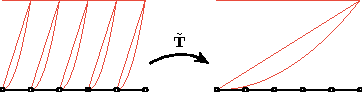
\includegraphics[scale=1.4]{algorithm_4_demo2}
		\caption{The operator $\tilde{\mathbf{T}}$ that maps piecewise polynomials to polynomials on the span $\left[s,e\right]$.}\label{fig:T-tilde}
	\end{subfigure}
	\begin{subfigure}{\linewidth}
		\center
		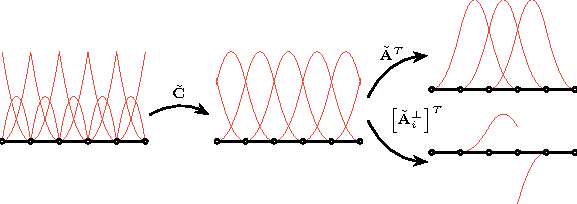
\includegraphics[scale=1.4]{algorithm_4_demo1}
		\caption{The block diagonal matrix $\tilde{\mathbf{C}}$ maps piece Bernstein basis functions to discontinuous B-spline basis functions, the assembly operator $\tilde{\mathbf{A}}$ constructed by restricting the operator $\mathbf{A}$ onto involved elements and spline basis functions maps discontinuous spline basis functions to continuous spline basis functions and the operator $\tilde{\mathbf{A}}^\perp_i$ constructed by restricting the operator $\mathbf{A}^\perp_i$ onto involved elements maps discontinuous spline basis functions to function $\tilde{N}_i$.}\label{fig:C_tilde_and_A_tilde}
	\end{subfigure}
	\caption{Illustration of behaviors of operators in Algorithm.~\ref{alg:modification_weight_new}. }
\end{figure}

The comparison of maximum condition numbers between the matrix $\mathbf{M}$ in Algorithm.~\ref{alg:modification_weight} and the matrix $\mathbf{M}$ in Algorithm.~\ref{alg:modification_weight_new} for constructing $p^\text{th}$ order dual basis function with $p^\text{th}$ order polynomial reproduction ($q=p$) is studied in Figure~\ref{fig:condition_number}. As can be seen, the condition number of $\mathbf{M}$ in Algorithm.~\ref{alg:modification_weight} grows at the rate $p$, whereas the condition number of $\mathbf{M}$ in Algorithm.~\ref{alg:modification_weight_new} is independent of mesh refinements. These results indicate the robustness of Algorithm.~\ref{alg:modification_weight_new}.

\begin{figure}[ht]
	\center
	\includestandalone[scale=1]{dual_basis_condition_number}%     without .tex extension
	% or use \input{mytikz}
	\caption{The growth of the maximum condition numbers of the matrix $\mathbf{M}$ in Algorithm.~\ref{alg:modification_weight} and Algorithm.~\ref{alg:modification_weight_new}.}
	\label{fig:condition_number}
\end{figure}

Thanks to Algorithm.~\ref{alg:modification_weight} and Algorithm.~\ref{alg:modification_weight_new}, the enriched dual basis reproduces polynomial globally (Assumption.~\ref{aspt:global_polynomial_reproduction}), and the construction process guarantees the supported of each enriched dual basis function consists no more than $p+q+1$ elements (Assumption.~\ref{aspt:local_support}). It remains to prove the local stability property (Assumption.~\ref{aspt:local_stability}).

\begin{proof}[Proof of Assumption.~\ref{aspt:local_stability}]
	\begin{align}
		\begin{split}
			\| \quasiid{N}u \|_{H^k(\Omega_e)} &= \| \sum_i \langle {N_i,u} \rangle_{\Omega}\hat{N}_i \|_{H^k(\Omega_e)}\\
			&\leq \| \sum_i \hat{N}_i\|_{H^k(\Omega_e)} \| \langle {\mathbf{N},u} \rangle_{\hat{\Omega}_e} \|_\infty\\
			&= \| \hat{\mathbf{N}}^T\mathbf{1} \|_{H^k(\Omega_e)} \| \langle {\mathbf{N},u} \rangle_{\hat{\Omega}_e} \|_\infty,
		\end{split}
	\end{align}
	where $\mathbf{1}$ is a unit valued vector of the same size as $\hat{\mathbf{N}}$. By rewriting $\hat{\mathbf{N}}$ in its expanded form~\eqref{eq:dual_basis_form}, we have
	\begin{equation}
		\| \quasiid{N}u \|_{H^k(\Omega_e)} \leq  \| \sum_i{B_i} \|_{H^k(\Omega_e)} \| \mathbf{G}^{-T}\mathbf{R}\mathbf{W}\mathbf{1} \|_\infty \| \langle {\mathbf{N},u} \rangle_{\hat{\Omega}_e} \|_\infty.
	\end{equation}
	From the definition of matrix norms, we then have
	\begin{equation}
		\begin{split}
			\| \quasiid{N}u \|_{H^k(\Omega_e)} &\leq \| \sum_i{B_i} \|_{H^k(\Omega_e)} \| \mathbf{G}^{-T}\mathbf{R}\mathbf{W}\|_\infty \| \langle {\mathbf{N},u} \rangle_{\hat{\Omega}_e} \|_\infty\\
			&\leq \| \sum_i{B_i} \|_{H^k(\Omega_e)} \| \mathbf{G}^{-T} \|_\infty \| \mathbf{R} \|_\infty \| \mathbf{W} \|_\infty \| \langle {\mathbf{N},u} \rangle_{\hat{\Omega}_e} \|_\infty.
		\end{split}\label{eq:proof_of_assumption3_1}
	\end{equation}

	Since Bernstein basis forms a partition of unity over each elements, we have that
	\begin{equation}
		\| \sum_i{B_i} \|_{H^k(\Omega_e)} = \| 1 \|_{H^k(\Omega_e)} = \| 1 \|_{L^2(\Omega_e)} = \sqrt{h}.\label{eq:proof_of_assumption3_2}
	\end{equation}

	Let $\mathbf{G}_{\left[ 0,1 \right]}$ be the Gramian matrix defined on the interval $\left[ 0,1 \right]$ and assume $\|\mathbf{G}^{-1}_{\left[ 0,1 \right]}\|_\infty = C_{gi}$, we have
	\begin{equation}
		\| \mathbf{G}^{-T} \|_\infty = \| \mathbf{G}^{-1} \|_\infty = h^{-1} \|\mathbf{G}^{-1}_{\left[ 0,1 \right]}\|_\infty = C_{gi}h^{-1}.\label{eq:proof_of_assumption3_3}
	\end{equation}

	Owing to the fact that the \Bezier element extraction operators are independent of the geometry and are invariant under uniform scaling, their norms are independent of the mesh size. In addition, there are finite number of different \Bezier element extraction operators generated by uniform mesh refinements. Hence, we can assume $\|\mathbf{R}\|_\infty=C_r$. Meanwhile, thanks to Algorithm.~\ref{alg:modification_weight_new}, the construction of $\mathbf{W}$ is geometry and mesh size independent. Hence, we can assume $\|\mathbf{W}\|_\infty=C_w$.\par

	Since spline basis functions are non-negative and also form a partition of unity, from Lemma.~\ref{lemma:local_polynomial_reproduction} and Cauchy-Schwarz inequality, we have that
	\begin{equation}
		\| \langle {\mathbf{N},u} \rangle_{\hat{\Omega}_e} \|_\infty \leq \| \langle {\mathbf{1},u} \rangle_{\hat{\Omega}_e} \|_\infty = \vert \int_{\hat{\Omega}_e} u d\Omega \vert \leq \|1\|_{L^2(\hat{\Omega}_e)} \|u\|_{L^2(\hat{\Omega}_e)}=\sqrt{C_m h} \|u\|_{L^2(\hat{\Omega}_e)}.\label{eq:proof_of_assumption3_4}
	\end{equation}
	where $C_m$ is the number of elements involed in $\hat{\Omega}_e$. By putting Equation~\eqref{eq:proof_of_assumption3_2}, \eqref{eq:proof_of_assumption3_3}, \eqref{eq:proof_of_assumption3_4} into Equation~\eqref{eq:proof_of_assumption3_1}, we have
	\begin{equation}
		\begin{split}
			\| \quasiid{N}u \|_{H^k(\Omega_e)} &\leq C_{gi}C_wC_r \sqrt{C_m} \|u\|_{L^2(\hat{\Omega}_e)} \\
			&\leq C_{gi}C_wC_r\sqrt{C_m}\|u\|_{H^k(\hat{\Omega}_e)}.
		\end{split}
	\end{equation}
	This ends the proof with $C_{st}=C_{gi}C_wC_r\sqrt{C_m}$.
\end{proof}
Hence, the enriched dual basis satisfies all assumptions and will yield optimal approximations. Figure~\ref{fig:enriched_basis_functions} gives an example of enriched \Bezier dual basis functions of the same primal B-spline basis function with different polynomial reproduction orders. As can be seen, the approximation power is improved at the expense of the support size.

\begin{figure}[ht]
	\center
	\begin{subfigure}[t]{.45\linewidth}
		\center
		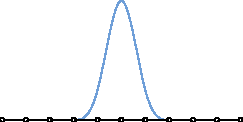
\includegraphics[width=.9\columnwidth]{p=3}
		\caption{A cubic B-spline function}\label{fig:a_cubic_spline}
	\end{subfigure}\\
	\begin{subfigure}[t]{.45\linewidth}
		\center
		\includegraphics[width=.9\columnwidth]{p=3_c=0}
		\caption{\Bezier dual basis function of~\ref{fig:a_cubic_spline}}
	\end{subfigure}\hfil
	\begin{subfigure}[t]{.45\linewidth}
		\center
		\includegraphics[width=.9\columnwidth]{p=3_c=1}
		\caption{Enriched \Bezier dual basis function of~\ref{fig:a_cubic_spline} that reproduces linear functions}
	\end{subfigure}\\
	\begin{subfigure}[t]{.45\linewidth}
		\center
		\includegraphics[width=.9\columnwidth]{p=3_c=2}
		\caption{Enriched \Bezier dual basis function of~\ref{fig:a_cubic_spline} that reproduces quadratic functions}
	\end{subfigure}\hfil
	\begin{subfigure}[t]{.45\linewidth}
		\center
		\includegraphics[width=.9\columnwidth]{p=3_c=3}
		\caption{Enriched \Bezier dual basis function of~\ref{fig:a_cubic_spline} that reproduces cubic functions}
	\end{subfigure}
	\caption{A cubic B-spline basis function and its corresponding enriched \Bezier dual basis functions with different polynomial reproduction orders. }\label{fig:enriched_basis_functions}
\end{figure}

\FloatBarrier

\section{Applications to $2^\text{nd}$ order and $4^\text{th}$ order mortar isogeometric analysis}\label{sec:dual_mortar}

The enriched dual basis functions can be used to discretize the Lagrange multiplier space for the constructing of constrained finite dimensional space in the dual mortar formulation. In this section, we demonstrate the dual mortar formulations of Poisson problem, linear elasticity problem and biharmonic problem. The formulations are grounded on a two-patch domain (see Figure~\ref{fig:two_patch_domain}) and the extension to multiple-patch domains is straightforward.

\begin{figure}[ht]
	\center
	\includegraphics[width=.7\columnwidth]{two_patch_domain}
	\caption{A two-patch planar domain $\Omega$ consisting of two patches $\Omega_s$ and $\Omega_m$. }\label{fig:two_patch_domain}
\end{figure}

\subsection{Vertex modification}

For a multi-patch decomposition, at least three patches meet at an interior vertex and several interfaces can share this vertex as a common endpoint. If we still discretize the Lagrange multiplier space with the same dimension as univariate basis of the slave side, we obtain too many constraints. Some of the control points in the neighborhood of a vertex may serve as both slave nodes and master nodes. As a result, the matrix $\mathbf{B}^\perp$ cannot be formed elegantly as Equation~\eqref{iii-eq:null-space}. In addition, it has been demonstrated in Chapter~\ref{chp:chapter3} that, such $\mathcal{V}^h$ constructed by global dual basis does not satisfy the \textit{inf-sup} condition, leading to a sub-optimal approximation error. Hence, vertex modifications are needed to relax overly constrained linear system.\par

In general, the vertex modification can be achieved by reducing the dimension of the Lagrange multiplier space. For second order problems, a Lagrange multiplier space of codimension $2$ of the trace space of the slave side is sufficient to remove redundant constraints; whereas, for fourth order problems, a Lagrange multiplier space of codimension $4$
of the trace space of the slave side is prefered. To construct an enriched dual basis of codimension $2c$, we remove the first $c$ and the last $c$ vectors in $\{\mathbf{A}_i\}_{i=0}^{n_N-1}$, leaving $\{\mathbf{A}_i\}_{i=c}^{n_N-1-c}$ a $n_N-2c$ dimensional vector space. The orthonormal vector basis of the null space of $\spn\{\mathbf{A}_i\}_{i=c}^{n_N-1-c}$ can be written as $\{\mathbf{A}^\perp_i\}_{i=0}^{n_B-n_N-1}\bigcup\{\mathbf{A}^n_i\}_{i=0}^{c-1}\bigcup\{\mathbf{A}^n_i\}_{i=n_N-c}^{n_N-1}$. Now, we can construct $\mathbf{W}^\text{ini}$ from $\{\mathbf{A}_i\}_{i=c}^{n_N-1-c}$ via Equation~\eqref{eq:initial_guess} and assemble $\mathbf{W}^\text{mod}$ from $\{\mathbf{A}^\perp_i\}_{i=0}^{n_B-n_N-1}\bigcup\{\mathbf{A}^n_i\}_{i=0}^{c-1}\bigcup\{\mathbf{A}^n_i\}_{i=n_N-c}^{n_N-1}$ via Algorithm.~\ref{alg:modification_weight_new}. The resulted dual basis is $2c$ dimensional less than the original basis and satisfies the global idempotence.

\subsection{Domain decomposition for $2^\text{nd}$ order problems}

Due to the existence of the first order weak derivative in the weak form of $2^\text{nd}$ order problems, the constrained space $\mathcal{V}^h$ should weakly satisfy $C^0$ continuity constraint across the interface $\Gamma$. Hence, the constrained space $\mathcal{V}^h$ for $2^\text{nd}$ order problems is given by

\begin{equation}
	\mathcal{V}^h\coloneqq \left\{ v\in \mathcal{X}^h \left|\quad \int_{\Gamma} \mu \left[ u \right] d \Gamma=0,\quad \forall \mu\in \mathcal{M}^h \right. \right\},
\end{equation}
where the Lagrange multiplier space $\mathcal{M}^h$ is two dimension less than the trace space of the slave side. As a result, in addition to the interface nodes of the master side, the first and the last interface nodes of the slave side also serve as master nodes (see Figure~\ref{fig:2nd_order_nodes}). 
\begin{figure}[ht]
	\center
	\includegraphics[width=.7\columnwidth]{two_patch_domain_poisson}
	\caption{The classification of nodes on the intersection for $2^\text{nd}$ order problems. }\label{fig:2nd_order_nodes}
\end{figure}

\subsection{Domain decomposition for $4^\text{th}$ order problems}

Due to the existence of the second order weak derivative in the weak form of $4^\text{nd}$ order problems, the constrained space $\mathcal{V}^h$ should weakly satisfy $C^1$ continuity constraint across the interface $\Gamma$. Hence, two Lagrange multiplier are needed to apply $C^0$ continuity constraint and $C^1$ continuity constraint, correspondingly. The constrained space $\mathcal{V}^h$ for $4^\text{nd}$ order problems is given by

\begin{equation}
	\mathcal{V}^h\coloneqq \left\{ v\in \mathcal{X}^h \left| \quad  \left\{\begin{alignedat}{2}
		&\int_{\Gamma} \mu_0 \left[ u \right] d \Gamma=0, &&\forall \mu_0\in \mathcal{M}_0^h\\
		&\int_{\Gamma} \mu_1 \left[ \frac{\partial u}{ \partial \xi_s} \right] d \Gamma=0\text{ if }\Gamma\parallel\eta_s\text{ or }\int_{\Gamma} \mu_1 \left[ \frac{\partial u}{ \partial \eta_s} \right] d\Gamma=0\text{ if }\Gamma\parallel\xi_s,\quad&&\forall\mu_1\in \mathcal{M}_1^h
	\end{alignedat}\right. \right. \right\},
\end{equation}
where both $\mathcal{M}_0^h$ and $\mathcal{M}_1^h$ are $4$ dimension less than the trace space of the slave side. As a result, four nodes in the neighborhood of each vertices of $\Omega_s$ are classified as master nodes.

\begin{figure}[ht]
	\center
	\includegraphics[width=.7\columnwidth]{two_patch_domain_biharmonic}
	\caption{The classification of nodes on the intersection for biharmonic problems ($4^\text{th}$ order problems). }
\end{figure}

\FloatBarrier

\section{Numerical examples}\label{sec:examples}

In this section, we investigate the performance of the enriched dual basis in several challenging $2^\text{nd}$ and $4^\text{th}$ order benchmarks. The first example is a Poisson's problem over a four-patch square domain, where the intersections are all non-matching parameterized. In the second problem, we model an infinite plate with a hole by four non-conforming NURBS patches. The third benchmark is a biharmonic over a five-patch square domain. A simply supported square Kirchhoff-Love plate is tested as our fourth example. To verify the robustness of enriched dual basis and dual mortar formulation for $4^\text{th}$ order problems, we consider the Cahn-Hilliard equation as the last benchmark. All numerical problem are solved by the Eigen library~\cite{eigenweb}. Due to the asymmetric structure of the consistency tangent matrix in Cahn-Hilliard problem, the BiCGSTAB solver is used whereas the conjugate gradient solver is used for the rest of problems. Note that extraordinary points are presented in all tested topologies. For the \Bezier dual basis, we adopt the extraordinary modification utilized in Chapter~\ref{chp:chapter3}.\par

Results obtained from the enriched dual basis are denoted by Enrich-$Q_i$. As a comparison, the performances of the enriched dual basis are compared with the global dual basis (labeled by $L^2$-$Q_i$) and the \Bezier dual basis (labeled by \Bezier-$Q_i$). For all $2^\text{nd}$ order problems, the polynomial reproduction order $q$ is set to $p-1$ for the construction of the $p^\text{th}$ order enriched dual basis whereas $q=p-2$ for all $4^\text{th}$ order problems. This setting ensures the sparsest stiffness matrix while maintains the optimality. All enriched dual basis are constructed via Algorithm.~\ref{alg:modification_weight_new}.

\subsection{Poisson problem}\label{sec:poisson_problem}

We start by solving the Poisson's equation $-\Delta u=f$ over the domain $\left[ 0, 1\right]\times \left[ 0, 1\right]$. The domain is decomposed into four patches, shown in Figure.~\ref{fig:Poisson_mesh}. The manufactured solution is given as:
\begin{equation}
	u(x,y) = \sin(2\pi x)\sin(2 \pi y).
\end{equation}
This manufactured solution satisfies the homogeneous Dirichlet boundary condition ($u=0$) and is demonstrated in Figure.~\ref{fig:Poisson_manufacture}.

\begin{figure}[ht]
	\center
	\begin{subfigure}[t]{.45\linewidth}
		\center
		\includegraphics[scale=1.35]{four_patches_nonconform_nonmatch}
		\caption{Non-matching parameterized non-conforming four-patch mesh}\label{fig:Poisson_mesh}
	\end{subfigure}
	\begin{subfigure}[t]{.45\linewidth}
		\center
		\includegraphics[scale=.41]{four_patches_solution-plot}
		\caption{The manufactured solution}\label{fig:Poisson_manufacture}
	\end{subfigure}
	\caption{The decomposition and discretization of the domain $\Omega=\left[ 0, 1\right]\times \left[ 0, 1\right]$ and the manufactured solution that satisfies $u=0$ on $\partial\Omega$, which are utilized as the initial mesh and the reference solution in Section~\ref{sec:poisson_problem}.}
\end{figure}

Convergence plots in $L^2$ norm and $H^1$ norm are shown in Figure.~\ref{fig:Poisson_convergence}. We observe optimal convergence of the enriched dual basis in all tested polynomial orders ($p=\left\{2,3,\dots,5\right\}$) in both measures. For $p=2,3$, the errors of the enriched dual basis are close to that of the global dual basis, whereas uniform shifts have been observed from the enriched dual basis of $p=4,5$. We speculate that the cause of vertical shifts of error curves is the non-matching parameterization. Since the enriched dual basis functions enjoy larger support size, the size of an extension element $\hat{\Omega}_e$ of the enriched dual basis will be significantly larger than that of the standard B-spline basis. As a result, the local estimation error of the enriched dual basis will be larger than that of the standard B-spline basis. And the irregular parameterization seems to aggravate this effect. Regardless of the slightly shift, however, the optimal convergence rates have been observed in both measures. The \Bezier dual basis, as expected, demonstrates sub-optimal convergence in both $L^2$ and $H^1$ for $p=3,4,5$. In addition, in the asymptotical region, the error increases as the polynomial order is increased.\par

\begin{figure}[ht]
	\center
	\captionsetup[subfigure]{labelformat=empty}
	\begin{subfigure}{.45\linewidth}
		\center
		\includestandalone[scale=.8]{four_patch_poisson_L2}
	\end{subfigure}\hspace{2mm}
	\begin{subfigure}{.45\linewidth}
		\center
		\includestandalone[scale=.8]{four_patch_poisson_H1}
	\end{subfigure}
	\caption{Convergence plots for non-matching parameterized non-conforming patch coupling in Section~\ref{sec:poisson_problem}. Left: error measured in $L^2$ norm. Right: error measured in $H^1$ norm.}\label{fig:Poisson_convergence}
\end{figure}

Contour plots of $\text{err} = u-u^h$ for cubic mesh after three refinements are shown in Figure.~\ref{fig:contour_Poisson}. As can be seen, the contour plot of the enriched dual basis is similar to that of the global dual basis, except some spikes in the neighbourhood of extraordinary points. On the other hand, a significant amount of oscillation is observed for the \Bezier dual basis along each intersection. It is deserved to notice that the in-domain error (approximation error) remains in the similar level as the other two cases.

\begin{figure}[ht]
	\center
	\captionsetup[subfigure]{labelformat=empty}
	\begin{subfigure}[t]{.45\linewidth}
		\center
		\includegraphics[scale=.52]{four_patch_poisson_op_contour}
		\caption{Enrich-$Q_3$}
	\end{subfigure}
	\begin{subfigure}[t]{.45\linewidth}
		\center
		\includegraphics[scale=.52]{four_patch_poisson_Bezier_contour}
		\caption{\Bezier-$Q_3$}
	\end{subfigure}\\
	\center
	\begin{subfigure}[t]{.45\linewidth}
		\center
		\includegraphics[scale=.52]{four_patch_poisson_L2_contour}
		\caption{$L^2$-$Q_3$}
	\end{subfigure}
	\caption{Contour plots of $\text{err} =u-u^h$ for the Poisson problem on the four-patch domain ($p=3$, and the mesh is obtained after three refinements). }\label{fig:contour_Poisson}
\end{figure}

\subsection{Linear elasticity -- plate with a hole}\label{sec:plate_with_a_hole}

To test the performance of the enriched dual basis over vector fields, we consider a linear elastic problem. The problem setup and the multi-patch discretization are demonstrated in Figure.~\ref{fig:plate_with_hole_setup}.  The traction along the outer edge is evaluated from the exact solution which is given by

\begin{align}
	\begin{split}
		\sigma_{rr}(r,\theta)&=\dfrac{T_x}{2}(1-\dfrac{R_1^2}{r^2})+\dfrac{T_x}{2}(1-4\dfrac{R_1^2}{r^2}+3\dfrac{R_1^4}{r^4})\cos(2\theta),\\
		\sigma_{\theta\theta}(r,\theta)&=\dfrac{T_x}{2}(1+\dfrac{R_1^2}{r^2})-\dfrac{T_x}{2}(1+3\dfrac{R_1^4}{r^4})\cos(2\theta),\\
		\sigma_{r\theta}(r,\theta)&=-\dfrac{T_x}{2}(1+2\dfrac{R_1^2}{r^2}-3\dfrac{R_1^4}{r^4})\sin(2\theta).
	\end{split}
\end{align}

\begin{figure}[ht]
	\captionsetup[subfigure]{width=0.9\textwidth}
	\center
	\begin{subfigure}[t]{.3\textwidth}
		\center
		\includegraphics[scale=.7]{Platewithhole}
		\caption{Infinite plate with a hole subjected to uniaxial tension at $x=\pm \infty$}
	\end{subfigure}
	\begin{subfigure}[t]{.3\textwidth}
		\center
		\includegraphics[scale=.7]{annular}
		\caption{The computational geometry, boundary conditions and material parameters. }
	\end{subfigure}
	\begin{subfigure}[t]{.3\textwidth}
		\center
		\includegraphics[scale=.45]{annular_mesh}
		\caption{The non-conforming four-patch mesh}
	\end{subfigure}
	\caption{The decomposition and discretization of the domain $\Omega$ and the manufactured solution that satisfies $u=0$ on $\partial\Omega$, which are utilized as the initial mesh and the reference solution in Section~\ref{sec:plate_with_a_hole}.}\label{fig:plate_with_hole_setup}
\end{figure}

The relative error of $\mathbf{u}$ are mesured in $L^2$ norm and energy semi-norm:
\begin{equation}
	\|\mathbf{u}-\mathbf{u}^h\|_{E}:=\sum_k\int_{\Omega_k}\frac{1}{2}\mathbf{\sigma}(\mathbf{u}-\mathbf{u}^h) \colon \mathbf{\epsilon}(\mathbf{u}-\mathbf{u}^h) d \Omega.
\end{equation}
Convergence plots for both measures are given in Figure.~\ref{fig:convergence_plate_with_hole}. Similar to the scalar problem, both the enriched dual basis and the global dual basis yield optimal convergence results for all tested polynomial orders in both measures. In addition, due to the absence of non-matching parameterized intersections, the convergence plots of the enriched dual basis are all identical to that of the global dual basis. The
convergence plots of the\Bezier dual basis, again, demonstrate sub-optimal performances.\par

\begin{figure}[ht]
	\center
	\captionsetup[subfigure]{labelformat=empty}
	\begin{subfigure}{.45\linewidth}
		\center
		\includestandalone[scale=.8]{four_patch_elasticity_L2}
	\end{subfigure}\hspace{2mm}
	\begin{subfigure}{.45\linewidth}
		\center
		\includestandalone[scale=.8]{four_patch_elasticity_energy}
	\end{subfigure}
	\caption{Convergence plots for simple non-conforming patch coupling in Section~\ref{sec:plate_with_a_hole}. Left: error measured in $L^2$ norm. Right: error measured in energy semi-norm.}\label{fig:convergence_plate_with_hole}
\end{figure}

Contour plots of $\text{err} = u_x - u_x^h$ at $p=3$ after three refinements are shown in Figure.~\ref{fig:contour_plate_with_hole}. As can be seen, the contour plots of both the enriched dual basis and the global dual basis are the same. The \Bezier dual basis, however, yields tremendous oscillation along each intersections. Again, the errors in each patch are in the similar level as for the global dual basis, which confirms that the main contribution of the sub-optimality is the consistency error.

\begin{figure}[ht]
	\center
	\captionsetup[subfigure]{labelformat=empty}
	\begin{subfigure}[t]{.45\linewidth}
		\center
		\includegraphics[scale=.4]{op_annular}
		\caption{Enrich-$Q_3$}
	\end{subfigure}
	\begin{subfigure}[t]{.45\linewidth}
		\center
		\includegraphics[scale=.4]{bezier_annular}
		\caption{\Bezier-$Q_3$}
	\end{subfigure}\\
	\center
	\begin{subfigure}[t]{.45\linewidth}
		\center
		\includegraphics[scale=.4]{l2_annular}
		\caption{$L^2$-$Q_3$}
	\end{subfigure}
	\caption{Contour plots of $\text{err} = u_x-u^h_x$ for the linear elastic problem on the four-patch domain ($p=3$, and the mesh is obtained after three refinements). }\label{fig:contour_plate_with_hole}
\end{figure}
\FloatBarrier

\subsection{Biharmonic problem}\label{sec:biharmonic_problem}

We next consider a homogeneous biharmonic problem over the domain $\left[0, 1\right]\times \left[0, 1\right]$, with the manufactured solution
\begin{equation}
	u(x,y)=\sin(2\pi{x})^2\sin(2\pi{y})^2.
\end{equation}
The discretization and the manufactured solution are depicted in Figure.~\ref{fig:biharmonic_mesh}.
\begin{figure}[ht]
	\center
	\begin{subfigure}[t]{.45\linewidth}
		\center
		\includegraphics[scale=1.35]{five_patches_mesh}
		\caption{Non-conforming five-patch mesh}
	\end{subfigure}
	\begin{subfigure}[t]{.45\linewidth}
		\center
		\includegraphics[scale=.425]{five_patch_solution-plot}
		\caption{The manufactured solution}
	\end{subfigure}
	\caption{The decomposition and discretization of the domain $\Omega$ and the manufactured solution that satisfies $u=\frac{\partial u}{\partial \mathbf{n}}=0$ on $\partial\Omega$, which are utilized as the initial mesh and the reference solution in Section~\ref{sec:biharmonic_problem}.}\label{fig:biharmonic_mesh}
\end{figure}

Convergence plots for the biharmonic benchmark are shown in Figure.~\ref{fig:convergence_biharmonic}. The enriched dual basis with $q=p-2$ generates optimal results for $p=2,3,4$ and the convergence plots are identical to that of the global dual basis. Note that the optimal convergence rate for quadratic basis functions is $\mathcal{O}(h^2)$ in $L^2$ norm for biharmonic problems. For the case of $p=5$, we observe sub-optimal convergence for both the enriched dual basis and the global dual basis at the last refinement in $L^2$ norm. However, no sub-optimality has been observed in $H^2$ norm. This phenomenon indicates that the error happens at certain digits of the floating point vector $\mathbf{U}^\text{mortar}$ (between $7^\text{th}$ and $10^\text{th}$ digit for this case). We infer that the cause of the sub-optimality is the conditioning of the stiffness matrix. In addition, studies~\cite{li2008effective} show that the growth rate of condition number for biharmonic problem is $\mathcal{O}(-h^4)$, which is huge, compared with $\mathcal{O}(-h^2)$ for Poisson's problem by finite element method. This explains why ill-conditioning of biharmonic problem happens much earlier than that of Poisson's problem. We also attribute the slightly better performance of the enriched dual basis functions to their compact support and the robust construction algorithm (Algorithm.~\ref{alg:modification_weight_new}). Again, the \Bezier dual basis leads to sub-optimal behavior for higher order elements.\par

\begin{figure}[ht]
	\center
	\captionsetup[subfigure]{labelformat=empty}
	\begin{subfigure}{.45\textwidth}
		\center
		\includestandalone[scale=.8]{five_patch_biharmonic_L2}
	\end{subfigure}\hspace{2mm}
	\begin{subfigure}{.45\textwidth}
		\center
		\includestandalone[scale=.8]{five_patch_biharmonic_H2}
	\end{subfigure}
	\caption{Convergence plots for five non-conforming patch coupling in Section~\ref{sec:biharmonic_problem}. Left: error measured in $L^2$ norm. Right: error measured in $H^2$ norm.}\label{fig:convergence_biharmonic}
\end{figure}

Contour plots for cubic mesh after two refinements are given in Figure.~\ref{fig:contour_biharmonic}. Similar to $2^\text{nd}$ order problems, the contour plot of the enriched dual basis is identical to that of the global dual basis, as the result of the absence of non-matching parameterized interfaces. However, due to the involving of control points that are one column away from the intersection, the consistency error of the \Bezier dual bais case penetrates into each patches for a relatively rough mesh.

\begin{figure}[ht]
	\center
	\captionsetup[subfigure]{labelformat=empty}
	\begin{subfigure}[t]{.45\linewidth}
		\center
		\includegraphics[scale=.52]{five_patch_biharmonic_op_contour}
		\caption{Prop-$Q_3$}
	\end{subfigure}
	\begin{subfigure}[t]{.45\linewidth}
		\center
		\includegraphics[scale=.52]{five_patch_biharmonic_Bezier_contour}
		\caption{\Bezier-$Q_3$}
	\end{subfigure}\\
	\center
	\begin{subfigure}[t]{.45\linewidth}
		\center
		\includegraphics[scale=.52]{five_patch_biharmonic_L2_contour}
		\caption{$L^2$-$Q_3$}
	\end{subfigure}
	\caption{Contour plots of $\text{err}=u-u^h$ for the biharmonic problem on the five-patch domain ($p=3$, and the mesh is obtained after two refinements). }\label{fig:contour_biharmonic}
\end{figure}


\subsection{Kirchhoff plate}\label{sec:kl-plate_problem}

The last benchmark with analytical solution is a simply supported square Kirchhoff plate. The bending moments of Kirchhoff plate is given by:
\begin{equation}
	\begin{split}
		M_{xx} &= -D\left( \frac{\partial^2 w}{\partial x^2} + \nu \frac{\partial^2 w}{\partial y^2}\right),\\
		M_{yy} &= -D\left( \frac{\partial^2 w}{\partial y^2} + \nu \frac{\partial^2 w}{\partial x^2}\right),\\
		M_{xy} &= -D(1-\nu) \frac{\partial^2 w}{\partial xy},
	\end{split}
\end{equation}
where $w$ is the vertical displacement, $D = \frac{Et^3}{12(1-\nu^2)}$, $t$ is the thickness, $E$ is the Young's modulus and $\nu$ is the Poisson's ratio. The governing equation of Kirchhoff plate can be derived as
\begin{equation}
	\frac{\partial^4 w}{\partial x^4} + \frac{\partial^4 w}{\partial x^2y^2} + \frac{\partial^4 w}{\partial y^4} = \frac{q}{D}
\end{equation}
where $q$ is the pressure. In this benchmark, we consider a square plate with $L=12$ subjected to a sinusoidal presure load of
\begin{equation}
	q(x,y) = -\sin(\frac{\pi x}{L}) \sin(\frac{\pi y}{L}).
\end{equation}
We also adopt $t=0.375$, $E=4.8\times 10^5$ and $\nu = 0.38$. The analytical solution is given by
\begin{equation}
	w(x, y) = -\frac{L^4}{4D\pi^4}\sin(\frac{\pi x}{L}) \sin(\frac{\pi y}{L}).
\end{equation}
The geometry, discretization and the analytical solution of vertical displacement are shown in Figure.~\ref{fig:kirchhoff_mesh}. Note that the green intersection is non-matching parameterized, whereas red curves are coupled non-comformingly. \par

\begin{figure}[ht]
	\center
	\begin{subfigure}[t]{.45\linewidth}
		\center
		\includegraphics[scale=.4]{plate_config-plot}
		\caption{Non-matching parameterized non-conforming three-patch mesh}
	\end{subfigure}
	\begin{subfigure}[t]{.45\linewidth}
		\center
		\includegraphics[scale=.3]{plate_solution-plot}
		\caption{The reference solution}
	\end{subfigure}
	\caption{The decomposition and discretization of the domain $\left[0, 1\right] \times \left[0, 1\right]$ and the refernce solution that satisfies $u=0$ on $\partial\Omega$ in Section~\ref{sec:kl-plate_problem}. The non-matching parameterized interface is denoted by green curve and the simple non-conforming discretized interfaces are denoted by red curves.}\label{fig:kirchhoff_mesh}
\end{figure}
Convergence behaviors of $w$, $M_{xx}$ and $M_{xy}$ are studied in Figure.~\ref{fig:convergence_kirchhoff}. As can be seen, both the enriched dual basis and the global dual basis yield optimal results for all polynomial orders in all three measures. As the biharmonic problem, ill-conditioning at the last refinement of $p=5$ is observed in $L^2$ norm whereas convergences of errors in $M_{xx}$ and $M_{xy}$ are still optimal. Due to the presence of a non-matching parameterized intersection, vertical shifts in error plots of the enriched dual basis have been observed for higher order elements ($p = 4,5$). Again, the \Bezier dual basis generates sub-optimal results. \par

\begin{figure}[ht]
	\center
	\captionsetup[subfigure]{labelformat=empty}
	\begin{subfigure}{.45\linewidth}
		\center
		\includestandalone[scale=.8]{three_patch_plate_L2}
	\end{subfigure}\hspace{2mm}
	\begin{subfigure}{.45\linewidth}
		\center
		\includestandalone[scale=.8]{three_patch_plate_Mx}
	\end{subfigure}\\
	\begin{subfigure}{.45\linewidth}
		\center
		\includestandalone[scale=.8]{three_patch_plate_Mxy}
	\end{subfigure}
	\caption{Convergence plots for the simply supported Kirchhoff plate in Section~\ref{sec:kl-plate_problem}. Upper left: error of $w$ measured in $L^2$ norm. Upper right: error of $M_{xx}$ measured in $L^2$ norm. Bottom: error of $M_{xy}$ measured in $L^2$ norm.}\label{fig:convergence_kirchhoff}
\end{figure}

Contour plots of $\text{err}=u_x-u_x^h$ for the simply supported Kirchhoff plate problem are given in Figure.~\ref{fig:contour_kirchhoff}. For the enriched dual basis and the global dual basis, no oscillation has been observed on the curved intersecitons, however, errors are evolved along the non-matching parameterized intersection. In addition, the influence of the non-matching intersection is more significant on the enriched dual basis case. For the case of the \Bezier dual basis, the consistency error is much higher and propagates into each patches.

\begin{figure}[ht]
	\center
	\captionsetup[subfigure]{labelformat=empty}
	\begin{subfigure}[t]{.45\linewidth}
		\center
		\includegraphics[scale=.4]{three_patch_plate_op_contour}
		\caption{Enrich-$Q_3$}
	\end{subfigure}
	\begin{subfigure}[t]{.45\linewidth}
		\center
		\includegraphics[scale=.4]{three_patch_plate_Bezier_contour}
		\caption{\Bezier-$Q_3$}
	\end{subfigure}\\
	\center
	\begin{subfigure}[t]{.45\linewidth}
		\center
		\includegraphics[scale=.4]{three_patch_plate_L2_contour}
		\caption{$L^2$-$Q_3$}
	\end{subfigure}
	\caption{Contour plots of $\text{err}=u_x-u_x^h$ for the simply supported Kirchhoff plate problem on the three-patch domain ($p=3$, and the mesh is obtained after two refinements). }\label{fig:contour_kirchhoff}
\end{figure}

\subsection{Cahn-Hilliard equation}

In this benchmark, we verify the robustness of the dual mortar method and the enriched dual basis by a $4^\text{th}$ order non-linear dynamic problem--Cahn-Hilliard equation. The Cahn-Hilliard equation is originally derived to model spinodal decomposition of binary mixtures. Taking the concentration $u$ of one of the mixtures's components as an phase-field parameter, the governing equation over infinite domain can be stated as
\begin{equation}
	\begin{split}
		\frac{\partial u}{\partial t} &= \nabla \cdot \left( M(u) \nabla\left( \mu(u)-\lambda \Delta u \right) \right)\text{ in } \Omega\times\left[ 0,T \right],\\
		u(\mathbf{x}, 0 ) &= u_0(\mathbf{x}) \text{ in } \Omega
	\end{split}
\end{equation}
where $M(u)$ is the mobility, $\mu(u)$ represents the chemical potential of a regular solution in the absence of phase interfaces and $\lambda$ is a positive constant such that $\sqrt{\lambda}$ represents a length scale of the problem. In this benchmark, we study the concentration distribution over a 2D domain with difference initial conditions and boundary conditions. We consider
\begin{align}
	M(u)   & = Du(1-u),                                                     \\
	\mu(u) & = 3\alpha\left(\frac{1}{2\theta}\log\frac{u}{1-u}+1-2u\right),
\end{align}
and adopt the following values: $\alpha=3000$, $D=1$, $\lambda = 1$ and $\theta = 1.5$. The weak form is stated as follows: find $u\in \mathcal{U}$ such that $\forall v\in \mathcal{V}$
\begin{equation}
	\langle \frac{\partial u}{\partial t}, v\rangle_\Omega + \langle M(u)\nabla \mu(u)+\nabla M(u)\Delta u,\nabla v \rangle_\Omega+\langle M(u)\Delta u,\Delta v \rangle_\Omega = 0,
\end{equation}
where $\mathcal{U}$ and $\mathcal{V}$ are suitable function spaces. \par

To achieve an optimal ratio of high-frequency and low-frequency dissipation, we adopt the first order generalized-$\alpha$ method~\cite{chung1993time, jansen2000generalized} as the temporal discretization scheme. In each time step, we require the nonlinear residual reduces to $10^{-4}$ of its initial value. For the sake of computational efficiency, we adopt an adaptive time stepping scheme introduced by G\'omez et al. in~\cite{gomez2008isogeometric}. This adaptive time stepping scheme takes advantage of the fact that the generalized-$\alpha$ method contains the backward Euler method as a special case, and use the relative error between solution from generalized-$\alpha$ method and solution from backward Euler method as an estimator of the current step size. \par

\subsubsection{Stochastic concentration distribution}

We first consider an initially stochastic concentration distribution over an infinite 2D domain, as:
\begin{equation}
	u_0(\mathbf{x}) = \bar{u}+r(\mathbf{x}),
\end{equation}
where $\bar{u}=0.63$ and the $r$ is a random variable with uniform distribution in the range $\left[ -0.005, 0.005 \right]$. The infinite domain can be described by a square domain $\Omega=\left[0 , 1\right] \times \left[0 , 1\right]$ with periodic boundary condition. Hence, for this case, both $\mathcal{U}$ and $\mathcal{V}$ are $H^2(\Omega)$ functions that satisfy periodic boundary condition. Taking into account that periodic boundary conditions are applied, it is anticipated that in the steady state only one circular inclusion remains. To demonstrate the robustness of the dual mortar method and the enriched dual basis, we non-uniformly discretize the domain $\Omega$ into $64 \times 64$ quadratic elements, the periodic boundary condition is applied by the dual mortar method.\par

The mesh and the structural evolution of the concentration distribution are demonstrated in Figure.~\ref{fig:phase_field_stochastic}. Note that both the top/bottom and the left/right interfaces are non-matching parameterized. As can be seen, from its initial stochastic pattern, the concentration distribution evolves into two phases whose composition is determined by the minima of the bulk free energy. The process is dominated by the reduction of the number of $u=0$ phase. Meanwhile, the characteristic length of $u=0$ phase is increased. Finially, the circular shape of the single inclusion is formed as the result of the bulk free energy minimization.

\begin{figure}[ht]
	\center
	\captionsetup[subfigure]{labelformat=empty}
	\begin{subfigure}[t]{.3\linewidth}
		\center
		\includegraphics[scale=.431]{phase_field_domain}
		\vspace{-.4\baselineskip}
		\caption{The distorted mesh}
	\end{subfigure}
	\begin{subfigure}[t]{.3\linewidth}
		\center
		\includegraphics[scale=.25]{stochastic_ch_1_2}
		\vspace{-.4\baselineskip}
		\caption{$t=0.000002$}
	\end{subfigure}
	\begin{subfigure}[t]{.3\linewidth}
		\center
		\includegraphics[scale=.25]{stochastic_ch_2_7}
		\vspace{-.4\baselineskip}
		\caption{$t=0.000007$}
	\end{subfigure}\\
	\vspace{.2\baselineskip}

	\begin{subfigure}[t]{.3\linewidth}
		\center
		\includegraphics[scale=.25]{stochastic_ch_3_15}
		\vspace{-.4\baselineskip}
		\caption{$t=0.000015$}
	\end{subfigure}
	\begin{subfigure}[t]{.3\linewidth}
		\center
		\includegraphics[scale=.25]{stochastic_ch_4_40}
		\vspace{-.4\baselineskip}
		\caption{{$t=0.000040$}}
	\end{subfigure}
	\begin{subfigure}[t]{.3\linewidth}
		\center
		\includegraphics[scale=.25]{stochastic_ch_5_82}
		\vspace{-.4\baselineskip}
		\caption{{$t=0.000082$}}
	\end{subfigure}\\
	\vspace{.2\baselineskip}

	\begin{subfigure}[t]{.3\linewidth}
		\center
		\includegraphics[scale=.25]{stochastic_ch_6_156}
		\vspace{-.4\baselineskip}
		\caption{$t=0.000156$}
	\end{subfigure}
	\begin{subfigure}[t]{.3\linewidth}
		\center
		\includegraphics[scale=.25]{stochastic_ch_7_2136}
		\vspace{-.4\baselineskip}
		\caption{{$t=0.002136$}}
	\end{subfigure}
	\begin{subfigure}[t]{.3\linewidth}
		\center
		\includegraphics[scale=.25]{stochastic_ch_8}
		\vspace{-.4\baselineskip}
		\caption{Steady state}
	\end{subfigure}
	\caption{Temporal evolution of an initially stochastic concentration distribution into phases of different composition. The periodic boundary conditions are applied by the dual mortar method with the enriched dual basis. The computational domain is non-uniformly discretized, mesh lines at $\xi=0.5$ and $\eta=0.5$ are highlighted.}\label{fig:phase_field_stochastic}
\end{figure}

\subsubsection{Linear concentration distribution}

In the second case, we do not take $\bar{u}$ as a constant, but we vary it linearly with the horizontal spatial coordinate from $0.1$ to $0.9$. The domain $\Omega = \left[ 0, 2 \right] \times \left[ 0, 2 \right]$ is decomposed into four patches that are coupled non-conformingly. In addition, to show the compatibility of the coupling method with other types of boundary condition, we consider
\begin{equation}
	\frac{ \partial u}{ \partial \mathbf{n}} = 0, \;\; \text{on }\partial \Omega.
\end{equation}
This boundary condition can be incorporated into the dual mortar formulation by solving localized null space problems over each extraordinary points on the boundary. \par

The mesh and the structural evolution of the concentration distribution are demonstrated in Figure.~\ref{fig:phase_field_linear}. Four patches are discretized into $63 \times 63$, $65 \times 65$, $65 \times 65$ and $63 \times 63$ cubic elements, correspondingly. In this case, three morphologies are formed in different regions of the domain. On the left-hand side of the domain, the red phase nucleates into the blue one. The exact opposite occurs on the right-hand side. In the middle, where $u\approx 0.5$, we observe the striped pattern typical from spinodal decomposition. Whereas the nucleation process is dominated in the middle region, the structural evolution at the boundaries $x = 0$ and $x = 2$ hardly exists. Eventually, the interface develops into a straight line at $x = 1$, which is consistent with the behavior of the exact solution.\par

In both cases, the convergence of the Newton's method is achieved within $3$ interations when $\Delta t<5\times 10^{-6}$ and $4$ interations when $5\times 10^{-6} \leq \Delta t < 1\times 10^{-4}$ for both the generalized-$\alpha$ method and the backward Euler method. This is the same as the simulation with one uniformly discretized patch. In addition, no influence in the time step size of the adaptive time stepping scheme has been observed. This confirms that the dual mortar method with the enriched dual basis does not impact the convergence behavior of the correction loop and the overall performance in solving nonlinear problems.

\begin{figure}[ht]
	\center
	\captionsetup[subfigure]{labelformat=empty}
	\begin{subfigure}[t]{.3\linewidth}
		\center
		\includegraphics[scale=.431]{phase_field_domain_linear}
		\vspace{-.4\baselineskip}
		\caption{The non-conforming four-patch mesh}
	\end{subfigure}
	\begin{subfigure}[t]{.3\linewidth}
		\center
		\includegraphics[scale=.25]{linear_ch_1_2}
		\vspace{-.4\baselineskip}
		\caption{$t=0.000002$}
	\end{subfigure}
	\begin{subfigure}[t]{.3\linewidth}
		\center
		\includegraphics[scale=.25]{linear_ch_2_4}
		\vspace{-.4\baselineskip}
		\caption{$t=0.000004$}
	\end{subfigure}\\
	\vspace{.2\baselineskip}

	\begin{subfigure}[t]{.3\linewidth}
		\center
		\includegraphics[scale=.25]{linear_ch_3_10}
		\vspace{-.4\baselineskip}
		\caption{$t=0.000010$}
	\end{subfigure}
	\begin{subfigure}[t]{.3\linewidth}
		\center
		\includegraphics[scale=.25]{linear_ch_4_48}
		\vspace{-.4\baselineskip}
		\caption{{$t=0.000048$}}
	\end{subfigure}
	\begin{subfigure}[t]{.3\linewidth}
		\center
		\includegraphics[scale=.25]{linear_ch_5_204}
		\vspace{-.4\baselineskip}
		\caption{{$t=0.000204$}}
	\end{subfigure}\\
	\vspace{.2\baselineskip}

	\begin{subfigure}[t]{.3\linewidth}
		\center
		\includegraphics[scale=.25]{linear_ch_6_1304}
		\vspace{-.4\baselineskip}
		\caption{$t=0.001304$}
	\end{subfigure}
	\begin{subfigure}[t]{.3\linewidth}
		\center
		\includegraphics[scale=.25]{linear_ch_7_5814}
		\vspace{-.4\baselineskip}
		\caption{{$t=0.005814$}}
	\end{subfigure}
	\begin{subfigure}[t]{.3\linewidth}
		\center
		\includegraphics[scale=.25]{linear_ch_8}
		\vspace{-.4\baselineskip}
		\caption{Steady state}
	\end{subfigure}
	\caption{Temporal evolution of an initially linear concentration distribution with stochastic perturbation into two phases separated by a straight interface. The four-patch domain are coupled by the dual mortar method with the enriched dual basis.}\label{fig:phase_field_linear}
\end{figure}
\FloatBarrier

\section{Conclusion}\label{sec:conlusion}

In this chapter, we develop an enrichment procedure to endow \Bezier dual basis functions with sufficient approximation ability. The cause of sub-optimal convergence of \Bezier dual basis is the lack of polynomial reproduction. The enriched \Bezier dual basis can reproduce polynomial up to a given order though at the expense of a slightly enlarged support size. Owing to the locality, the linear system from static condensation remains sparse. The proposed enrichment methodology is based on the formulation in Oswald et al.~\cite{oswald2001polynomial} and two significant improvements have been made in efficiency and robustness aspects. The proposed formulation is quadrature-free and independent of the mesh size. Hence, the cost in assembly different operators will be eliminated and the effect of the problem scale on the conditioning these operators will be minimized, giving rise to a more efficient and robust formulation. \par

The performance of the enriched \Bezier dual basis is demonstrated via several challenging benchmark problems. These problems include $2^\text{nd}$ order, $4^\text{th}$ order, linear, nonlinear, static and dynamic problems. The proposed dual basis demonstrates optimal convergence and yields compelling results as compared with the global dual basis. The robustness of the proposed dual basis is also confirmed by two highly nonlinear dynamic phase-field problems.\par

% Finally, although the proposed enrichment procedure cures the sub-optimality of \Bezier dual basis at the expense of a slightly enlarged support, we believe there exists a better formulation that can achieve the same performance without any influences on the support size. This is subjected to the future research.
% \chapter{Kirchhoff-Love shell problem}
\label{chp:chapter5}
\graphicspath{{figures/}{figures/chapter5/}}
\pgfplotsset{
	table/search path={{figures/chapter5/data},{data}},
}

\section{Dual mortar method for non-homogeneous constraints}\label{sec:dual_mortar}

We briefly demonstrate the dual mortar method in the context of an abstract formulation for a constrained problem: find $u\in\mathcal{X}$ and $\lambda\in\mathcal{M}$ such that
\begin{subequations}\label{eq:LM-form-non-hom}
	\begin{empheq}[left=\empheqlbrace]{alignat=2}
		a(v,u)+b(v,\lambda)&=l(v)\quad &&\forall{}v\in\mathcal{X},\\
		b(\mu,u)&=c(\mu)\quad &&\forall{}\mu\in\mathcal{M},\label{eq:LM-form-constraint-non-hom}
	\end{empheq}.
\end{subequations}
%%TODO: which section
where $a(\cdot,\cdot)$ is a bilinear form representing a potential energy, $l(\cdot)$ is a linear form representing the external load, $b(\cdot,\cdot)$ is a bilinear form representing a set of constraints on the solution $u$ and $c(\mu)$ is a linear form corresponding to any non-homogeneous constraints. In Section~, $b(\cdot,\cdot)$ and $c(\cdot)$ will represent the continuity constraints across patch boundaries for each Newton-Raphson iteration.

If we introduce a pair of discrete function spaces $\mathcal{X}^h \subset \mathcal{X}$ and $\mathcal{M}^h \subset \mathcal{M}$ we can represent the weak form~\eqref{eq:LM-form-non-hom} as the matrix problem
\begin{equation}\label{eq:disc-LM-form-non-hom}
	\mathbf{K}^\text{LM}\mathbf{U}^{\text{LM}}=\begin{bmatrix}
		\mathbf{K} & \mathbf{B}^T \\
		\mathbf{B} & \mathbf{0}
	\end{bmatrix}\mathbf{U}^{\text{LM}}
	=
	\begin{bmatrix}
		\mathbf{F} \\
		\mathbf{R}
	\end{bmatrix},
\end{equation}
where $\mathbf{K}$ is the discretized stiffness matrix, $\mathbf{F}$ is the discretized external force vector, $\mathbf{B}$ is the discretized constraints matrix, $\mathbf{R}$ is the forcing term due to non-homogeneous constraints (for homogeneous constraints, $\mathbf{R} = \mathbf{0}$) and $\mathbf{U}^{\text{LM}}$ is a vector containing the control values $\mathbf{U}$ of the displacement field and the control values $\mathbf{\Lambda}$ Lagrange multiplier field. The mortar method statically condenses out additional unknowns and gives rise to a positive definite variational problem by introducing a constrained function space
\begin{equation}
	\mathcal{V}^h\coloneq\{u^h\in\mathcal{X}^h\, | \, b(\lambda^h,u^h)=0, \quad \forall{}\lambda^h\in\mathcal{M}^h\}.
\end{equation}
The saddle point problem~\eqref{eq:LM-form-non-hom} can now be transformed into a minimization problem: find a general solution $u^h_\text{hom}\in\mathcal{V}^h$ such that, for $u^h = u^h_\text{hom}+ u^h_\text{non}$
\begin{equation}
	a(v^h, u^h)=l(v^h),\quad \forall{}v^h\in\mathcal{V}^h,
\end{equation}
where $u^h_\text{non}\in \mathcal{X}^h$ is a particular solution that satisfies the constraint~\eqref{eq:LM-form-constraint-non-hom}. Given $\mathbf{N}^{\mathcal{X}^h}$, the vector containing the basis functions of $\mathcal{X}^h$, the vector containing the basis functions of $\mathcal{V}^h$ is given by
\begin{equation}
	\mathbf{N}^{\mathcal{V}^h}=\left[\mathbf{B}^\perp\right]^T\mathbf{N},\label{eq:basis-null-space-non-hom}
\end{equation}
where the matrix $\mathbf{B}^\perp$ is the vector basis of the null space of the constraint matrix $\mathbf{B}$. If the Lagrange multiplier space is discretized by a set of dual basis functions, the constraint matrix $\mathbf{B}$ can be written as~\cite{gilbert1987computing}
\begin{equation}\label{eq:constraint-form-non-hom}
	\mathbf{B}=\begin{bmatrix}
		\mathbf{I} & \mathbf{B_2}
	\end{bmatrix},
\end{equation}
the bandwidth of $\mathbf{B}_2$ depends on the support size of dual basis functions. \par

For a $\mathbf{B}$ in the form~\eqref{eq:constraint-form-non-hom}, the vector basis of its null space can be obtained from
\begin{equation}
	\mathbf{B}^\perp=\begin{bmatrix}
		-\mathbf{B}_2 \\
		\mathbf{I}
	\end{bmatrix}.
	\label{eq:null-space-non-hom}
\end{equation}
The discretization of the constraint~\eqref{eq:LM-form-constraint-non-hom} is
\begin{equation}
	\mathbf{B}\mathbf{U}^\text{non} = \mathbf{R},
\end{equation}
where a particular solution can be solved from~\cite{ainsworth2001essential}
\begin{equation}
	\mathbf{U}^\text{non} = \mathbf{B}^T\left[ \mathbf{B}\mathbf{B}^T \right]^{-1}\mathbf{R}.
\end{equation}
However, for a constraint matrix takes the form~\eqref{eq:constraint-form-non-hom}, a particular solution can be explicitly constructed as
\begin{equation}
	\mathbf{U}^\text{non} = \begin{bmatrix}
		\mathbf{R} \\\mathbf{0}
	\end{bmatrix}.\label{eq:dual_particular_solution}
\end{equation}
The mortar linear system can now be written as
\begin{equation}
	\mathbf{K}^{\text{mortar}}\mathbf{U}^{\text{mortar}}=\left[\mathbf{B}^\perp\right]^T\mathbf{K}\mathbf{B}^\perp\mathbf{U}^{\text{mortar}}=\left[\mathbf{B}^\perp\right]^T\mathbf{F}-\left[\mathbf{B}^\perp\right]^T\mathbf{K}\mathbf{U}^\text{non}.\label{eq:mortar-form-discretized}
\end{equation}
The relation between the mortar displacement nodal value vector $\mathbf{U}^{\text{mortar}}$, non-homogeneous solution $\mathbf{U}^\text{non}$ and $\mathbf{U}$ is given by
\begin{equation}
	\mathbf{U}=\mathbf{B}^\perp\mathbf{U}^{\text{mortar}}+\mathbf{U}^\text{non}.
\end{equation}
With a sparse $\mathbf{B}^\perp$ obtained from a set of dual basis with compact support, the stiffness matrix of the mortar formulation $\mathbf{K}^{\text{mortar}}$ will remain sparse, resulting in an efficient linear system.

\section{Formulation of Kirchhoff-Love shell}\label{sec:formulation}

In this section, we present the formulation of Kirchhoff-Love shell in compact form. The theory of Kirchhoff-Love shell is based on the assumption that the normal of the shell's mid-surface remains perpendicular in the deformed configuration. Hence, the strain the transverse strains are zero and the description of shell geometry can be reduced to its mid-surface.

\subsection{Kinematics}\label{sec:kinematics}

In what follows, we use Greek letters for indices taking values $\left\{1, 2\right\}$ and Latin letters for $\left\{1,2,3\right\}$, respectively. Einstein summation convention on repeated indices is also utilized. We now consider a shell structure of arbitrary geometry with constant thickness $h$ and parameterized with curvilinear coordinates $\theta^i$, where $\theta^1$ and $\theta^2$ denote the natural curvilinear coordinates and $\theta^3$ indicates the thickness direction with $\theta^3\in \left[-0.5h, \; 0.5h\right]$ (see Figure~\ref{fig:shell_configuration}). We use $\mathbf{R}(\theta^1,\theta^2), \mathbf{r}(\theta^1,\theta^2)\colon \mathbb{R}^2\rightarrow\mathbb{R}^3$ to describe the mid-surface of a shell in reference and current configurations, respectively. For simplicity and without loss of generality, we assume the parametric domain $\hat{\Omega}=[0,1]\times[0,1]$. The displacement of the shell mid-surface is given by
\begin{equation}
	\label{}
	\mathbf{u}(\theta^1,\theta^2) = \mathbf{r}(\theta^1,\theta^2)-\mathbf{R}(\theta^1,\theta^2).
\end{equation}
The mid-surface covariant base vectors in both configurations are obtained by
\begin{equation}
	\label{eq:mid_surface_base_vector}
	\begin{cases}
		\begin{aligned}
			\mathbf{A}_\alpha & =\mathbf{R}_{,\alpha} = \frac{\partial\mathbf{R}}{\partial\theta^\alpha}            \\
			\mathbf{A}_3      & = \frac{\mathbf{A}_1\times\mathbf{A}_2}{\vert{\mathbf{A}_1\times\mathbf{A}_2}\vert}
		\end{aligned}
	\end{cases},\qquad
	\begin{cases}
		\begin{aligned}
			\mathbf{a}_\alpha & =\mathbf{r}_{,\alpha} = \frac{\partial\mathbf{r}}{\partial\theta^\alpha}  =  \mathbf{A}_\alpha+\mathbf{u}_{,\alpha} \\
			\mathbf{a}_3      & = \frac{\mathbf{a}_1\times\mathbf{a}_2}{\vert{\mathbf{a}_1\times\mathbf{a}_2}\vert}
		\end{aligned}
	\end{cases},
\end{equation}
where $\vert\cdot\vert$ denotes the Euclidean length of the given vector. $\mathbf{A}_3$ and $\mathbf{a}_3$ are commonly refered to as the directors in the reference and currect configurations. The position vector of any material point within the shell in both reference configuration and current configuration are described by
\begin{equation}
	\label{eq:position_vector}
	\begin{cases}
		\begin{aligned}
			\mathbf{X}(\theta^1, \theta^2, \theta^3) & = \mathbf{R}(\theta^1, \theta^2) + \theta^3\mathbf{A}_3(\theta^1,\theta^2) \\
			\mathbf{x}(\theta^1, \theta^2, \theta^3) & = \mathbf{r}(\theta^1, \theta^2) + \theta^3\mathbf{a}_3(\theta^1,\theta^2)
		\end{aligned}
	\end{cases},
\end{equation}
Similar to the mid-surface, the covariant base vectors at any arbitrary material point within the shell in two configurations are obtained by
\begin{equation}
	\label{eq:base_vector}
	\begin{cases}
		\begin{aligned}
			\mathbf{G}_\alpha & =\mathbf{X}_{,\alpha} = \mathbf{A}_\alpha+\theta^3\mathbf{A}_{3,\alpha} \\
			\mathbf{G}_3      & = \mathbf{X}_{,3} = \mathbf{A}_3
		\end{aligned}
	\end{cases},\qquad
	\begin{cases}
		\begin{aligned}
			\mathbf{g}_\alpha & =\mathbf{x}_{,\alpha} = \mathbf{a}_\alpha+\theta^3\mathbf{a}_{3,\alpha} \\
			\mathbf{g}_3      & = \mathbf{x}_{,3} = \mathbf{a}_3
		\end{aligned}
	\end{cases}.
\end{equation}


\begin{figure}[h]
	\center
	\includestandalone[scale=1]{configuration}%     without .tex extension
	% or use \input{mytikz}
	\caption{Illustration of deformation, reference and currect configuration of Kirchhoff-Love shell. The mid-surface is denoted by blue color.}
	\label{fig:shell_configuration}
\end{figure}
The covariant and contravariant metric coefficients are computed by
\begin{equation}
	\label{eq:covariant_contravariant_metric}
	\begin{cases}
		\begin{aligned}
			G_{ij} & =\mathbf{G}_i\cdot\mathbf{G}_j \\
			G^{ij} & =\left[G_{ij}\right]^{-1}
		\end{aligned}
	\end{cases},\qquad
	\begin{cases}
		\begin{aligned}
			A_{ij} & =\mathbf{A}_i\cdot\mathbf{A}_j \\
			A^{ij} & =\left[A_{ij}\right]^{-1}
		\end{aligned}
	\end{cases},\qquad
	\begin{cases}
		\begin{aligned}
			g_{ij} & =\mathbf{g}_i\cdot\mathbf{g}_j \\
			g^{ij} & =\left[g_{ij}\right]^{-1}
		\end{aligned}
	\end{cases},\qquad
	\begin{cases}
		\begin{aligned}
			a_{ij} & =\mathbf{a}_i\cdot\mathbf{a}_j \\
			a^{ij} & =\left[a_{ij}\right]^{-1}
		\end{aligned}
	\end{cases}.
\end{equation}
The contravariant base vectors are then given by
\begin{equation}
	\label{eq:contravariant_base_vector}
	\mathbf{G}^i = G^{ij}\mathbf{G}_j,\qquad \mathbf{A}^i = A^{ij}\mathbf{A}_j,\qquad \mathbf{g}^i = g^{ij}\mathbf{g}_j,\qquad \mathbf{a}^i = a^{ij}\mathbf{a}_j.
\end{equation}

Form the numerour strain measures, we use the \textit{Green-Lagrangian} strain tensor to describe the strain, which is defined as
\begin{equation}
	\label{eq:green_lagrangian}
	\mathbf{E} = \frac{1}{2}\left( \mathbf{F}^T\mathbf{F}-\mathbf{I} \right),
\end{equation}
where $\mathbf{F}=\frac{\partial \mathbf{x}}{\partial \mathbf{X}}=\mathbf{g}_i\otimes\mathbf{G}^i$ is the deformation gradient and $\mathbf{I}$ is the identity tensor. Alternatively, $\mathbf{E}$ can be represented as
\begin{equation}
	\label{eq:green_lagrangian_contravariant}
	\mathbf{E}=E_{ij}\mathbf{G}^i\otimes\mathbf{G}^j,\quad\text{with } E_{ij} = \frac{1}{2}\left( g_{ij}-G_{ij} \right).
\end{equation}
Substituting~\eqref{eq:covariant_contravariant_metric} into~\eqref{eq:green_lagrangian_contravariant}, we obtain $E_{i3}=E_{3i}=0$. Separating the strain into a constant part due to membrane load and alinear part due to bending and neglecting $\bigO((\theta^3)^2)$ terms, the rest strain coefficients are given by
\begin{equation}
	\label{}
	E_{\alpha\beta} = \epsilon_{\alpha\beta} + \theta^3\kappa_{\alpha\beta},
\end{equation}
where the membrane strain tensor
\begin{equation}
	\label{eq:membrane_strains}
	\mathbf{\epsilon} = \epsilon_{\alpha\beta}\mathbf{G}^\alpha\otimes\mathbf{G}^\beta, \quad\epsilon_{\alpha\beta} = \frac{1}{2}\left( a_{\alpha\beta}-A_{\alpha\beta} \right) = \frac{1}{2}\left( \mathbf{a}_{\alpha}\cdot\mathbf{a}_{\beta}-\mathbf{A}_{\alpha}\cdot\mathbf{A}_{\beta} \right),
\end{equation}
and the tensor expressing changes in curvature
\begin{equation}
	\label{eq:curvatures}
	\mathbf{\kappa} = \kappa_{\alpha\beta}\mathbf{G}^\alpha\otimes\mathbf{G}^\beta,\quad\kappa_{\alpha\beta} = b_{\alpha\beta}-B_{\alpha\beta},\qquad\text{with }
	\begin{cases}
		\begin{aligned}
			B_{\alpha\beta} & =\frac{1}{2}\left( \mathbf{A}_{\alpha}\cdot\mathbf{A}_{3,\beta}+\mathbf{A}_{\beta}\cdot\mathbf{A}_{3,\alpha}\right) = -\mathbf{A}_{\alpha,\beta}\cdot\mathbf{A}_3 \\
			b_{\alpha\beta} & =\frac{1}{2}\left( \mathbf{a}_{\alpha}\cdot\mathbf{a}_{3,\beta}+\mathbf{a}_{\beta}\cdot\mathbf{a}_{3,\alpha}\right)  =-\mathbf{a}_{\alpha,\beta}\cdot\mathbf{a}_3
		\end{aligned}
	\end{cases}.
\end{equation}

\subsection{Equilibrium of elastic Kirchhoff-Love shell}\label{sec:equilibrium}

Next, we develop the variational formulation from the minimization of the potential energy. For the sake of simplicity, we assume that the shell is linear elastic with a strain energy density per unit area of the form~\cite{chapelle2010finite}
\begin{equation}
	\label{eq:strain_energy_density}
	W(\theta^1,\theta^2) = \frac{1}{2}\left( h \mathbf{\epsilon}\colon \mathbf{C}\colon \mathbf{\epsilon} + \frac{h^3}{12} \mathbf{\kappa }\colon \mathbf{C}\colon \mathbf{\kappa } \right)= \frac{1}{2}\left( hC^{\alpha\beta\gamma\delta}\epsilon_{\alpha\beta}\epsilon_{\gamma\delta}+\frac{h^3}{12}C^{\alpha\beta\gamma\delta}\kappa_{\alpha\beta}\kappa_{\gamma\delta} \right),
\end{equation}
where $E$ is Young's modulus, $\nu$ is Poisson's ratio and the fourth order material tensor
\begin{equation}
	\label{eq:material_tensor}
	\mathbf{C} = C^{\alpha\beta\gamma\delta} \mathbf{A}_\alpha\otimes\mathbf{A}_\beta\otimes\mathbf{A}_\gamma\otimes\mathbf{A}_\delta,\qquad C^{\alpha\beta\gamma\delta} = \frac{E\nu}{1-\nu^2} A^{\alpha\beta}A^{\gamma\delta}+\frac{E}{2(1+\nu)}\left( A^{\alpha\gamma}A^{\beta\delta}+A^{\alpha\delta}A^{\beta\gamma} \right).
\end{equation}
The membrane force resultants tensor and the bending moment resultants tensor read
\begin{equation}
	\label{eq:stress_and_moment}
	\begin{cases}
		\begin{aligned}
			\mathbf{n} & = n^{\alpha\beta}\mathbf{A}_\alpha\otimes\mathbf{A}_\beta,\quad n^{\alpha\beta} =\frac{\partial W}{\partial \epsilon_{\alpha\beta}} = hC^{\alpha\beta\gamma\delta}\epsilon_{\gamma\delta}         \\
			\mathbf{m} & = m^{\alpha\beta}\mathbf{A}_\alpha\otimes\mathbf{A}_\beta,\quad m^{\alpha\beta} =\frac{\partial W}{\partial \kappa_{\alpha\beta}} =\frac{h^3}{12}C^{\alpha\beta\gamma\delta}\kappa_{\gamma\delta}
		\end{aligned}
	\end{cases}.
\end{equation}
The potential energy of Kirchhoff-Love shell is defined as
\begin{equation}
	\label{eq:potential_energy}
	\Pi(\mathbf{u},\mathbf{u}) = \Pi^\text{int}(\mathbf{u},\mathbf{u})+\Pi^\text{ext}(\mathbf{f}, \mathbf{u}) = \int_{\overline{\Omega}}W d\Omega+\Pi^\text{ext}(\mathbf{f}, \mathbf{u}),
\end{equation}
where $\overline{\Omega}$ is the mid-surface of the shell in the reference configuration, $d\Omega=\vert{\mathbf{A}_1\times\mathbf{A}_2}\vert d\theta^1 d\theta^2$ is the differential area, $\Pi^\text{int}(\mathbf{u},\mathbf{u}) = \int_{\overline{\Omega}}W d\Omega$ is the strain energy and $\Pi^\text{ext}(\mathbf{f},\mathbf{u})$ is the external work due to external force $\mathbf{f}$, in general $\Pi^\text{ext}$ is a linear functional with respect to $\mathbf{u}$. The variation formulation can be obtained from the minimization of the potential energy,
\begin{equation}
	\label{eq:weak_form_nonlinear}
	\delta \Pi(\mathbf{u},\delta\mathbf{u}) = \frac{\partial \Pi}{\partial \mathbf{u}} \delta\mathbf{u} = \int_{\overline{\Omega}} \left(\delta{\epsilon(\mathbf{u},\delta\mathbf{u})} \colon\mathbf{n}(\mathbf{u}) + \delta{\kappa(\mathbf{u},\delta\mathbf{u})} \colon \mathbf{m}(\mathbf{u}) \right)d \Omega+\Pi^\text{ext}(\mathbf{f},\delta\mathbf{u})= 0,
\end{equation}
with
\begin{equation}
	\label{}
	\delta{\epsilon(\mathbf{u},\delta\mathbf{u})} = \frac{\partial \mathbf{\epsilon}(\mathbf{u})}{\partial \mathbf{u}}\delta\mathbf{u},\qquad \text{and }\delta{\kappa(\mathbf{u},\delta\mathbf{u})} = \frac{\partial \mathbf{\kappa}(\mathbf{u})}{\partial \mathbf{u}}\delta\mathbf{u}.
\end{equation}
However, the variational formulation~\eqref{eq:weak_form_nonlinear} is a nonlinear functional with respect to $\mathbf{u}$ and cannot be solved directly. Hence, we adopt the Newton-Raphson method to solve the problem iteratively. Assuming $\mathbf{u}^{i+1} = \mathbf{u}^{i} +{\Delta} \mathbf{u}$, the weak form for solving ${\Delta} \mathbf{u}$ is stated as: find ${\Delta}\mathbf{u}\in \boldsymbol{\mathcal{X}}$, such that
\begin{equation}
	\label{eq:weak_form_linearized}
	\left(K_\text{m}(\mathbf{u}^i,\delta\mathbf{u},\Delta\mathbf{u})+K_\text{b}(\mathbf{u}^i,\delta\mathbf{u},\Delta\mathbf{u})\right)=-\delta \Pi(\mathbf{u}^{i},\delta\mathbf{u}),\qquad \forall \delta\mathbf{u}\in \boldsymbol{\mathcal{X}},
	% -\int_\Omega \left(\delta{\epsilon(\mathbf{u}_{i},\delta\mathbf{u})} \colon \delta\mathbf{n}(\mathbf{u}_i,{\Delta}\mathbf{u}) + \delta{\epsilon(\mathbf{u}_{i},\delta\mathbf{u},\Delta\mathbf{u})} \colon \mathbf{n}(\mathbf{u}_i) + \delta{\kappa(\mathbf{u}_i,\delta\mathbf{u})} \colon \delta\mathbf{m}(\mathbf{u}_i,{\Delta}\mathbf{u}) \right)d \Omega = \delta \Pi(\mathbf{u}_{i},\delta\mathbf{u}),\qquad \forall \delta\mathbf{u}\in \mathbf{\mathcal{U}},
\end{equation}
where $i$ denotes the iterative step, the solution space $\boldsymbol{\mathcal{X}}=\left[H^2(\hat{\Omega})\right]^3$, the membrane stiffness
\begin{equation}
	K_\text{m}(\mathbf{u}^i,\delta\mathbf{u},\Delta\mathbf{u}) = \int_{\overline{\Omega}} \delta{\epsilon(\mathbf{u}^{i},\delta\mathbf{u})} \colon \delta\mathbf{n}(\mathbf{u}^i,{\Delta}\mathbf{u}) + \delta{\epsilon(\mathbf{u}^{i},\delta\mathbf{u},\Delta\mathbf{u})} \colon \mathbf{n}(\mathbf{u}^i) d\Omega,
\end{equation}
and the bending stiffness
\begin{equation}
	K_\text{b}(\mathbf{u}^i,\delta\mathbf{u},\Delta\mathbf{u}) = \int_{\overline{\Omega}} \delta{\kappa(\mathbf{u}^{i},\delta\mathbf{u})} \colon \delta\mathbf{m}(\mathbf{u}^i,{\Delta}\mathbf{u}) + \delta{\kappa(\mathbf{u}^{i},\delta\mathbf{u},\Delta\mathbf{u})} \colon \mathbf{m}(\mathbf{u}^i) d\Omega,
\end{equation}
with
\begin{equation}
	\begin{cases}
		\begin{aligned}
			\delta{\mathbf{n}(\mathbf{u},{\Delta}\mathbf{u})}              & = \frac{\partial \mathbf{n}(\mathbf{u})}{\partial \mathbf{u}}{\Delta}\mathbf{u} = h\mathbf{C}\colon \delta\mathbf{\epsilon}(\mathbf{u},\Delta\mathbf{u}), \\
			\delta{\mathbf{m}({\Delta}\mathbf{u})}                         & = \frac{\partial \mathbf{m}}{\partial \mathbf{u}}{\Delta}\mathbf{u} = \frac{h^3}{12}\mathbf{C}\colon \delta\mathbf{\kappa}(\Delta\mathbf{u}),             \\
			\delta{\epsilon(\mathbf{u},\delta\mathbf{u},\Delta\mathbf{u})} & = \frac{\partial \delta\mathbf{\epsilon}(\mathbf{u},\delta\mathbf{u})}{\partial \mathbf{u}}\Delta\mathbf{u},                                              \\
			\delta{\kappa(\mathbf{u},\delta\mathbf{u},\Delta\mathbf{u})}   & = \frac{\partial \delta\mathbf{\kappa}(\mathbf{u},\delta\mathbf{u})}{\partial \mathbf{u}}\Delta\mathbf{u}.
		\end{aligned}
	\end{cases}
\end{equation}

\section{A dual mortar formulation for the multi-patch Kirchhoff-Love shell}\label{sec:multi_patch}

Most of the commonly used patch coupling approaches for Kirchhoff-Love shell fall into the following categories: penalty method~\cite{kiendl2010bending, herrema2019penalty}, Lagrange multiplier method (collocation approach can be viewed as a Lagrange multiplier method with the Lagrange multiplier discretized by Dirac delta functions )~\cite{coox2017flexible, hirschler2019embedded, schuss2019multi, goyal2017penalty}, and Nitsche's method~\cite{guo_nitsches_2015, nguyen2017isogeometric}. The performance of the penalty method is significantly influenced by the choice of the penalty parameter: a small penalty parameter cannot effectively enforce inter-patch constraint while a large penalty parameter may badly affect the condition number of the linear system. Usually, the selection of the penalty parameter is performed empirically by the analyst. The Lagrange multiplier methods leads to a saddle point problem, for with iterative methods are known to be less efficient than for symmetric positive definite systems. In addition, redundancy may happen in the discretized constraint matrix, leading to a rank deficiency linear system (\textit{inf-sup} instability). Although a global factorization followed by a static condensation can circumvent this issue, the resulted linear system no longer preserves its sparsity and may be polluted by the numerical error within the factorization process. The stability parameter in the Nitsche method needs to be approximated by eigenvalue problems associated with element intersections, which increase the computational cost. For nonlinear problems, the Nitsche's method becomes complex as it requires the tractions and their variations on the interface. \par

Here, we present a dual mortar formulation for the Kirchhoff-Love shell over multi-patch tensor product domains. Thanks to the locally supported dual basis, the linear system can be statically condensed with minimum computational cost and the resulted linear system preserves its sparsity. Along each interface, we introduce a local coordinate system, in which a generic inter-patch constraint is developed in a natural manner. The main advantages of this generic inter-patch constraint are that it deals with both patches joining smoothly and those joining at a kink in a uniform framework and it is compatible with dual basis.\par

We first introduce a rotation operator: for a vector $\mathbf{v}\in\mathbb{R}^3$, its rotation round the axis $\mathbf{k}\in\mathbb{R}^3$ by an angle $\theta$ according to the right hand rule is given as
\begin{equation}
	\mathbf{R}_{\mathbf{k},\theta}(\mathbf{v}) = \mathbf{v}\cos(\theta)+\left(\frac{\mathbf{k}}{\vert \mathbf{k} \vert}\times \mathbf{v}\right)\sin(\theta)+\frac{\mathbf{k}}{\vert \mathbf{k} \vert}\left(\frac{\mathbf{k}}{\vert \mathbf{k} \vert}\cdot\mathbf{v}\right)(1-\cos(\theta)). \label{eq:rodrigues_rotation}
\end{equation}
This operator is called the Rodrigues' rotation formula~\cite{rodrigues1840lois} and will play an important rule in formulating the inter-patch constraint.\par

To demonstrate our approach, we consider a kinked shell structure consisting of two NURBS patches shown in Figure~\ref{fig:two_patch_shell_with_kink}. We denote by $\Omega_s$ the slave domain, $\Omega_m$ the master domain and $\Gamma_{sm}$ the intersection between two patches. These two domains are parameterized by coordinate systems $(\theta^1_s, \theta^2_s)$ and $(\theta^1_m, \theta^2_m)$, respectively.

\begin{figure}[ht]
	\center
	\includegraphics[width=.5\columnwidth]{two_patch_shell_with_kink}
	\caption{A two-patch non-conforming Kirchhoff-Love shell consisting of two patches $\Omega_s$ and $\Omega_m$ with the intersection denoted by the red curve. The director $\mathbf{A}_3^m$ of $\Omega_m$ and the director $\mathbf{A}_3^s$ of $\Omega_s$ determine a rotation angle $\theta$ along the intersection. }\label{fig:two_patch_shell_with_kink}
\end{figure}

\subsection{A local coordinate system for patch intersections}

\begin{table}
	\center
	\caption{The strategy in selecting the restrictions of $\bar{\theta}^1$ and $\bar{\theta}^2$ on $\Omega_s$, where $\bar{\mathbf{A}}_\alpha^k=\sfrac{\partial\mathbf{X}^k}{\partial \bar{\theta}^\alpha\vert_{\Omega_k}}$}
	\label{tab:orientation_and_coordinate}
	\begin{tabularx}{.5\textwidth}{l@{\extracolsep{\fill}}cc}
		\toprule
		Interface orientation & $\bar{\theta}^1\vert_{\Omega_s}$         & $\bar{\theta}^2\vert_{\Omega_s}$         \\
		\midrule
		South                 & $\bar{\mathbf{A}}_1^s = -\mathbf{A}_2^s$ & $\bar{\mathbf{A}}_2^s = \mathbf{A}_1^s$  \\
		East                  & $\bar{\mathbf{A}}_1^s = \mathbf{A}_1^s$  & $\bar{\mathbf{A}}_2^s = \mathbf{A}_2^s$  \\
		North                 & $\bar{\mathbf{A}}_1^s = \mathbf{A}_2^s$  & $\bar{\mathbf{A}}_2^s = -\mathbf{A}_1^s$ \\
		West                  & $\bar{\mathbf{A}}_1^s = -\mathbf{A}_1^s$ & $\bar{\mathbf{A}}_2^s = -\mathbf{A}_2^s$ \\
		\bottomrule
	\end{tabularx}
\end{table}

In this subsection, we reparameterize the intersection between the slave patch and the master patch by a coordinate system $(\bar{\theta}^1, \bar{\theta}^2)$. However, we do not need to develop explicitly the map from $(\bar{\theta}^1, \bar{\theta}^2)$ to $\Omega_s$ and $\Omega_m$. Instead, we are interested in the covariant base vectors $(\bar{\mathbf{A}}_1, \bar{\mathbf{A}}_2)$ defined in the new coordinate system and how they behave during the deformation. The new coordinate system is defined based on the orientation of both the slave patch and the master path. We first specify the restrictions of $\bar{\theta}^1$ and $\bar{\theta}^2$ on $\Omega_s$ following the strategy given in Table~\ref{tab:orientation_and_coordinate}. For example, if an intersection is a north edge on the slave patch, we have
\begin{equation}
	\left\{
	\begin{split}
		\bar{\mathbf{A}}^s_1 &= \frac{\partial\mathbf{X}^s}{\partial \bar{\theta}^1\vert_{\Omega_s}} = \begin{bmatrix}
			\mathbf{A}_1^s & \mathbf{A}_2^s
		\end{bmatrix} \cdot \mathbf{J}_{\bar{\theta}^1}\vert_{\Omega_s} = \mathbf{A}_2^s\\
		\bar{\mathbf{A}}_2^s &= \frac{\partial\mathbf{X}^s}{\partial \bar{\theta}^2\vert_{\Omega_s}} = \begin{bmatrix}
			\mathbf{A}_1^s & \mathbf{A}_2^s
		\end{bmatrix} \cdot \mathbf{J}_{\bar{\theta}^2}\vert_{\Omega_s} = -\mathbf{A}_1^s
	\end{split}
	\right.,
\end{equation}
with
\begin{equation}
	\left\{
	\begin{split}
		\mathbf{J}_{\bar{\theta}^1}\vert_{\Omega_s} &=
		\begin{bmatrix}
			\frac{\partial \theta^1_s}{\partial \bar{\theta}^1\vert_{\Omega_s}} \\
			\frac{\partial \theta^2_s}{\partial \bar{\theta}^1\vert_{\Omega_s}}
		\end{bmatrix}=
		\begin{bmatrix}
			0 \\
			1
		\end{bmatrix}\\
		\mathbf{J}_{\bar{\theta}^2}\vert_{\Omega_s} &= \begin{bmatrix}
			\frac{\partial \theta^1_s}{\partial \bar{\theta}^2\vert_{\Omega_s}} \\
			\frac{\partial \theta^2_s}{\partial \bar{\theta}^2\vert_{\Omega_s}}
		\end{bmatrix}=
		\begin{bmatrix}
			-1 \\
			0
		\end{bmatrix}
	\end{split}
	\right..
\end{equation}

For different pairings of the slave edge and the master edge, the corresponding Jacobian $\mathbf{J}_{\bar{\theta}^1}\vert_{\Omega_s}$, $\mathbf{J}_{\bar{\theta}^2}\vert_{\Omega_s}$ can be computed in the same manner. \par

We now extend the curvilinear coordinate system $(\bar{\theta}^1, \bar{\theta}^2)$ from the slave patch to the master patch. A natural choice of the restriction of $\bar{\theta}^2$ on $\Omega_m$ is
\begin{equation}
	\bar{\theta}^2\vert_{\Omega_m}=\bar{\theta}^2\vert_{\Omega_s}, \text{ or } \bar{\mathbf{A}}^m_2=\bar{\mathbf{A}}^s_2.
\end{equation}
Given the directors $\mathbf{A}^s_3$ and $\mathbf{A}^m_3$ and the axis $\bar{\mathbf{A}}^s_2$, we can now uniquely determine the counterclockwise rotation (see Figure~\ref{fig:two_patch_shell_with_kink}) from $\mathbf{A}^m_3$ to $\mathbf{A}^s_3$ by
\begin{equation}
	\left\{
	\begin{split}
		\cos{\theta} &= \mathbf{A}^m_3\cdot \mathbf{A}^s_3\\
		\sin{\theta} &= \frac{(\bar{\mathbf{A}}^m_2 \times \mathbf{A}^m_3) \cdot \mathbf{A}^s_3}{\vert \bar{\mathbf{A}}^m_2 \vert}.
	\end{split}
	\right.\label{eq:rotation_angle}
\end{equation}
By Equation~\eqref{eq:rodrigues_rotation}, we can define a rotation operator rotate $\mathbf{A}^s_3$ to $\mathbf{A}^m_3$ around the axis $\bar{\mathbf{A}}^m_2$ as
\begin{equation}
	\mathbf{A}^m_3 = \mathbf{R}_{\bar{\mathbf{A}}^m_2,-\theta}(\mathbf{A}^s_3) =  -\mathbf{R}_{\bar{\mathbf{A}}^m_2,\theta}(\mathbf{A}^s_3).
\end{equation}
Meanwhile, the rotation operator $\mathbf{R}_{\bar{\mathbf{A}}^m_2,-\theta}$ also rotates $\bar{\mathbf{A}}^s_1$ to the tangential plane of $\Omega_m$ along the intersection. We let
\begin{equation}
	\bar{\mathbf{A}}^m_1=\mathbf{R}_{\bar{\mathbf{A}}^m_2,-\theta}(\bar{\mathbf{A}}^s_1).\label{eq:reference_constraint_c1}
\end{equation}
The corresponding Jacobians $\mathbf{J}_{\bar{\theta}^1}\vert_{\Omega_m} = \begin{bmatrix}
		\frac{\partial \theta^1_m}{\partial \bar{\theta}^1\vert_{\Omega_m}} & \frac{\partial \theta^2_m}{\partial \bar{\theta}^1\vert_{\Omega_m}}
	\end{bmatrix}^T$ and $\mathbf{J}_{\bar{\theta}^2}\vert_{\Omega_m} = \begin{bmatrix}
		\frac{\partial \theta^1_m}{\partial \bar{\theta}^2\vert_{\Omega_m}} & \frac{\partial \theta^2_m}{\partial \bar{\theta}^2\vert_{\Omega_m}}
	\end{bmatrix}^T$ are given by
\begin{equation}
	\begin{split}
		\begin{bmatrix}
			\mathbf{A}_1^m & \mathbf{A}_2^m
		\end{bmatrix} \cdot \mathbf{J}_{\bar{\theta}^1}\vert_{\Omega_m} &= \mathbf{R}_{\bar{\mathbf{A}}^m_2,-\theta}(\bar{\mathbf{A}}^s_1),\\
		\begin{bmatrix}
			\mathbf{A}_1^m & \mathbf{A}_2^m
		\end{bmatrix} \cdot \mathbf{J}_{\bar{\theta}^2}\vert_{\Omega_m} &= \bar{\mathbf{A}}^s_2.
	\end{split}\label{eq:jacobian_of_Jtheta}
\end{equation}
As $\begin{bmatrix}
		\mathbf{A}_1^m & \mathbf{A}_2^m
	\end{bmatrix}$ is a $3\times 2$ matrix, Equation~\eqref{eq:jacobian_of_Jtheta} could not be factorized directly. However, as $\mathbf{R}_{\bar{\mathbf{A}}^m_2,-\theta}(\bar{\mathbf{A}}^s_1)$ and $\bar{\mathbf{A}}^s_2$ are on the tangential plane of $\Omega_m$, we can solve $\mathbf{J}_{\bar{\theta}^1}\vert_{\Omega_m}$ and $\mathbf{J}_{\bar{\theta}^2}\vert_{\Omega_m}$ by
\begin{equation}
	\begin{split}
		\mathbf{J}_{\bar{\theta}^1}\vert_{\Omega_m} &= \left(\begin{bmatrix}
			\mathbf{A}_1^m & \mathbf{A}_2^m
		\end{bmatrix}^T\cdot\begin{bmatrix}
			\mathbf{A}_1^m & \mathbf{A}_2^m
		\end{bmatrix}\right)^{-1}\left(\begin{bmatrix}
			\mathbf{A}_1^m & \mathbf{A}_2^m
		\end{bmatrix}^T\cdot\mathbf{R}_{\bar{\mathbf{A}}^m_2,-\theta}(\bar{\mathbf{A}}^s_1) \right),\\
		\mathbf{J}_{\bar{\theta}^2}\vert_{\Omega_m} &= \left(\begin{bmatrix}
			\mathbf{A}_1^m & \mathbf{A}_2^m
		\end{bmatrix}^T\cdot\begin{bmatrix}
			\mathbf{A}_1^m & \mathbf{A}_2^m
		\end{bmatrix}\right)^{-1}\left(\begin{bmatrix}
			\mathbf{A}_1^m & \mathbf{A}_2^m
		\end{bmatrix}^T\cdot\bar{\mathbf{A}}^s_2 \right).
	\end{split}
\end{equation}

Following the above procedures, we have that the covariant base vectors of the master patch are nothing but the rotation of the covariant base vectors of the slave patch via the rotation operator $\mathbf{R}_{\bar{\mathbf{A}}^m_2,-\theta}$ (see Figure~\ref{fig:coordinate_system_on_each_patch}), as
\begin{equation}
	\begin{bmatrix}
		\bar{\mathbf{A}}_1^m & \bar{\mathbf{A}}_2^m
	\end{bmatrix}
	=
	\begin{bmatrix}
		\mathbf{R}_{\bar{\mathbf{A}}^m_2,-\theta}(\bar{\mathbf{A}}_1^s) & \bar{\mathbf{A}}_2^s
	\end{bmatrix}
	=
	\mathbf{R}_{\bar{\mathbf{A}}^m_2,-\theta}
	\begin{bmatrix}
		\bar{\mathbf{A}}_1^s & \bar{\mathbf{A}}_2^s
	\end{bmatrix}.
\end{equation}

The partial derivatives of the displacement $\mathbf{u}$ w.r.t. the new coordinate system $(\bar{\theta}^1, \bar{\theta}^2)$ are now given by
\begin{equation}
	\left\{
	\begin{split}
		\bar{\mathbf{u}}^s_{,1} &= \frac{\partial \mathbf{u}^s}{\partial \bar{\theta}^1\vert_{\Omega_s}} = \begin{bmatrix}
			\mathbf{u}^s_{,1} & \mathbf{u}^s_{,2}
		\end{bmatrix}\mathbf{J}_{\bar{\theta}^1}\vert_{\Omega_s}\\
		\bar{\mathbf{u}}^m_{,1} &= \frac{\partial \mathbf{u}^m}{\partial \bar{\theta}^1\vert_{\Omega_m}} = \begin{bmatrix}
			\mathbf{u}^m_{,1} & \mathbf{u}^m_{,2}
		\end{bmatrix}\mathbf{J}_{\bar{\theta}^1}\vert_{\Omega_m}\\
		\bar{\mathbf{u}}^m_{,2} &= \frac{\partial \mathbf{u}^m}{\partial \bar{\theta}^2\vert_{\Omega_m}} = \begin{bmatrix}
			\mathbf{u}^m_{,1} & \mathbf{u}^m_{,2}
		\end{bmatrix}\mathbf{J}_{\bar{\theta}^2}\vert_{\Omega_m}
	\end{split}
	\right..
\end{equation}

\begin{figure}[ht]
	\centering
	\begin{subfigure}[t]{0.4\textwidth}
		\centering
		\includegraphics[scale = .7]{master_patch}
		\caption{Slave patch}
	\end{subfigure}
	\begin{subfigure}[t]{0.58\textwidth}
		\centering
		\includegraphics[trim=.2cm .5cm 0 0, clip, scale = .9]{slave_patch}
		\caption{Master patch}
	\end{subfigure}
	\caption{ The covariant base vectors $(\bar{\mathbf{A}}_1, \bar{\mathbf{A}}_2)$ of the coordinate system $(\bar{\theta}^1, \bar{\theta}^2)$ on both the slave patch and the master patch. Note that the covariant base vectors of the master patch can be obtained by rotating the covariant base vectors of the slave patch via the rotation operator $\mathbf{R}_{\bar{\mathbf{A}}^m_2,-\theta}$. }\label{fig:coordinate_system_on_each_patch}
\end{figure}

\begin{remark}
	Following the strategy in Table~\ref{tab:orientation_and_coordinate} is of crucial importance with respect to the algorithm's stability. Figure~\ref{fig:parametric_of_slave_master} shows the restriction of the new coordinate system on the coupling edges for different coupling scenarios. As can be seen, the new coordinate system always follows the right hand rule. On the slave patch, $\bar{\theta}^1$ is always perpendicular to $\bar{\theta}^2$, while on the master patch, $\bar{\theta}^1$ and $\bar{\theta}^2$ forms an angle in the range of $(0^{\circ}, 180^{\circ})$. Thus, the director of the new coordinate system is always consistent with the director of the original coordinate system, i.e.
	\begin{equation}
		\left\{
		\begin{split}
			\bar{\mathbf{A}}^s_3 &= {\mathbf{A}}^s_3\\
			\bar{\mathbf{A}}^m_3 &= {\mathbf{A}}^m_3
		\end{split}
		\right..\label{eq:A3_consistency}
	\end{equation}
	On the contrary, if we do not follow the scheme in Table~\ref{tab:orientation_and_coordinate}, the new coordinate system may not obey the right hand rule, Equation~\eqref{eq:A3_consistency} may not be satisfied and the rotation angle from Equation~\eqref{eq:rotation_angle} may not necessarily guide $\bar{\mathbf{A}}^s_1$ to the tangential plane of $\Omega_m$.
\end{remark}

\begin{figure}[ht]
	\centering
	\begin{subfigure}[b]{0.47\textwidth}
		\centering
		\includestandalone[scale=.9]{master_coordinates}
		\caption{Parametric domain of the master patch}
	\end{subfigure}
	\begin{subfigure}[b]{0.47\textwidth}
		\centering
		\includestandalone[scale=.9]{slave_coordinates}
		\caption{Parametric domain of the slave patch}
	\end{subfigure}
	\caption{The new coordinate system $(\bar{\theta}^1, \bar{\theta}^2)$ on parametric domains of both slave patch and master patch. Coordinate systems on different edges denote the orientations in different coupling scenarios. Note that no matter which edge is coupled, the new coordinate system always obey the right hand rule on both slave and master patches.}
	\label{fig:parametric_of_slave_master}
\end{figure}

\subsection{Generic dual-compatible constraints for Kirchhoff-Love shell coupling}

Shell patches can be coupled smoothly as well as joined at a kink. In this subsection, we propose a set of constraints that can tackle shell coupling in a systematic manner. Compared with existing Kirchhoff-Love shell continuity constraints, the proposed formulation has its uniqueness. For instance, the constraint proposed in~\cite{schuss2019multi} only deal with $G^1$ continuity of adjacent patches, while the proposed formulation can tackle shell patches joined at different angle in a uniform framework. When patches are coupled smoothly, the proposed constraints will enforce $C^1$ continuity across adjacent patches while the angle between directors of adjacent patches will be preserved when they are joined at a kink. The constraint presented in~\cite{coox_robust_2017, hirschler2019embedded} is designed for small deformation problems, while the proposed formulation solves both small deformation and large deformation problems. In addition, the proposed constraints are compatible with dual basis, i.e. the discretized constraint matrix takes the form of Equation~\eqref{eq:constraint-form-non-hom}, and the \textit{inf-sup} stability is automatically satisfied.\par

In the coordinate system $(\bar{\theta}^1, \bar{\theta}^2)$, two physical properties that satisfied in the reference configuration should be preserved:
\begin{subequations}
	\begin{align}
		\mathbf{X}^s-\mathbf{X}^m=0\quad                                                              & \Rightarrow\quad \mathbf{x}^s-\mathbf{x}^m=0,\label{eq:preserve_c0}                                                               \\
		\bar{\mathbf{A}}^s_3 - \mathbf{R}_{\bar{\mathbf{A}}^m_2,\theta}(\bar{\mathbf{A}}^m_3)=0 \quad & \Rightarrow\quad \bar{\mathbf{a}}^s_3 - \mathbf{R}_{\bar{\mathbf{a}}^m_2,\theta}(\bar{\mathbf{a}}^m_3) = 0,\label{eq:preserve_c1}
	\end{align}
\end{subequations}
where Equation~\eqref{eq:preserve_c0} indicates the continuity of the displacement and Equation~\eqref{eq:preserve_c1} reflects the rotational continuity between two patches. Equation~\eqref{eq:preserve_c1} can be applied directly to classic Lagrange multiplier formulation, however, for dual mortaring, modifications are required to fully take the advantage of dual basis functions.\par

We modify Equation~\eqref{eq:preserve_c1} by the following steps:
\begin{equation}
	\bar{\mathbf{a}}^s_3 - \mathbf{R}_{\bar{\mathbf{a}}^m_2,\theta}(\bar{\mathbf{a}}^m_3) = 0 \supset \bar{\mathbf{a}}^s_1 \times \bar{\mathbf{a}}^s_2 - \mathbf{R}_{\bar{\mathbf{a}}^m_2,\theta}(\bar{\mathbf{a}}^m_1 \times \bar{\mathbf{a}}^m_2) = 0\supset \bar{\mathbf{a}}^s_1 - \mathbf{R}_{\bar{\mathbf{a}}^m_2,\theta}(\bar{\mathbf{a}}^m_1) = 0,
\end{equation}
where the symbol $\supset$ indicates that functions that satisfy the equation on the right-hand side is a subset of those on the left-hand side. Combining Equation~\eqref{eq:reference_constraint_c1}, we have:
\begin{equation}
	\bar{\mathbf{A}}^s_1 - \mathbf{R}_{\bar{\mathbf{A}}^m_2,\theta}(\bar{\mathbf{A}}^m_1) = 0 \quad \Rightarrow\quad \bar{\mathbf{a}}^s_1 - \mathbf{R}_{\bar{\mathbf{a}}^m_2,\theta}(\bar{\mathbf{a}}^m_1) = 0.\label{eq:preserve_c1_dual}
\end{equation}
Subtracting two equations in Equation~\eqref{eq:preserve_c0} and~\eqref{eq:preserve_c1_dual} respectively, we obtain:
\begin{subequations}
	\begin{align}
		\mathbf{u}^s-\mathbf{u}^m=0,\label{eq:constraint_c0_kl} \\
		\bar{\mathbf{u}}^s_{,1} - \mathbf{R}_{\bar{\mathbf{a}}^m_2,\theta}(\bar{\mathbf{a}}^m_1) + \mathbf{R}_{\bar{\mathbf{A}}^m_2,\theta}(\bar{\mathbf{A}}^m_1) = 0.\label{eq:constraint_c1_kl}
	\end{align}
\end{subequations}

Note that, for two patches that are coupled smoothly, i.e. $\theta=0$, Equation~\eqref{eq:constraint_c1_kl} reduces to
\begin{equation}
	\bar{\mathbf{u}}^s_{,1} - \mathbf{R}_{\bar{\mathbf{a}}^m_2,0}(\bar{\mathbf{a}}^m_1) + \mathbf{R}_{\bar{\mathbf{A}}^m_2,0}(\bar{\mathbf{A}}^m_1) = \bar{\mathbf{u}}^s_{,1} - \bar{\mathbf{a}}^m_1 + \bar{\mathbf{A}}^m_1 = \bar{\mathbf{u}}^s_{,1} - \bar{\mathbf{u}}^m_{,1} = 0,\label{eq:constraint_c1_kl_smooth}
\end{equation}
which is indeed the $C^1$ continuity condition in the coordinate system $(\bar{\theta}^1, \bar{\theta}^2)$. Both Equation~\eqref{eq:constraint_c0_kl} and Equation~\eqref{eq:constraint_c1_kl_smooth} are linear. To solve the nonlinear problem at $\mathbf{u}^{i+1} = \mathbf{u}^{i} +{\Delta} \mathbf{u}$, we have
\begin{subequations}
	\begin{align}
		\Delta\mathbf{u}^s-\Delta\mathbf{u}^m=0, \\
		\Delta\bar{\mathbf{u}}^s_{,1} - \Delta\bar{\mathbf{u}}^m_{,1} = 0.
	\end{align}
\end{subequations}
However, when patches coupled at a kink, the constraint~\eqref{eq:constraint_c1_kl} is no longer linear. Hence, the Newton-Raphson method is needed to apply the constraint~\eqref{eq:constraint_c1_kl} iteratively. as
\begin{equation}
	\Delta\bar{\mathbf{u}}^s_{,1}-\frac{\partial \mathbf{R}_{\bar{\mathbf{a}}^m_2,\theta}(\bar{\mathbf{a}}^m_1)}{\partial \mathbf{u}^m}\Delta\bar{\mathbf{u}}^m_{,1} = \mathbf{r}_c^i,\quad\text{with}\quad \mathbf{r}_c^i = -\left[\bar{\mathbf{a}}^s_1 - \mathbf{R}_{\bar{\mathbf{a}}^m_2,\theta}(\bar{\mathbf{a}}^m_1)\right]_{\mathbf{u}=\mathbf{u}^{i}}.
\end{equation}

\begin{remark}
	It is important to use $\bar{\mathbf{a}}^m_2$ as the rotation axis in the rotation operator formulation of Equation~\eqref{eq:preserve_c1_dual}. Although $\bar{\mathbf{a}}^s_2$ equals to $\bar{\mathbf{a}}^m_2$ in the weak sense, the presence of $\Delta\bar{\mathbf{u}}^s_{,2}$ in the linearization of $\bar{\mathbf{a}}^m_2$ will impede the formulation of the identity submatrix in Equation~\eqref{eq:constraint-form-non-hom}.
\end{remark}

\subsection{The dual mortar formulation}

The Lagrange multiplier formulation for the multi-patch nonlinear Kirchhoff-Love shell can be stated as: find $\Delta\mathbf{u} \in \boldsymbol{\mathcal{X}}$, $\boldsymbol{\lambda}_0\in\boldsymbol{\mathcal{M}}_0 $ and $\boldsymbol{\lambda}_1\in\boldsymbol{\mathcal{M}}_1$ such that
\begin{subequations}
	\begin{empheq}[left=\empheqlbrace]{alignat=2}
		K_\text{m}(\mathbf{u}^i,\delta\mathbf{u},\Delta\mathbf{u})+K_\text{b}(\mathbf{u}^i,\delta\mathbf{u},\Delta\mathbf{u})+b_0(\boldsymbol{\lambda}_0,\delta\mathbf{u})+b_1(\mathbf{u}^i, \boldsymbol{\lambda}_1,\delta\mathbf{u}) & =-\delta \Pi(\mathbf{u}^{i},\delta\mathbf{u})\quad      & \forall \delta\mathbf{u}              & \in{\boldsymbol{\mathcal{X}}},   \\
		b_0(\delta\boldsymbol{\lambda}_0,\Delta\mathbf{u})                                                                                                                                                                            & =0 \quad                                                & \forall \delta\boldsymbol{\lambda}_0  & \in{\boldsymbol{\mathcal{M}}_0},\label{eq:mixed_c0_constraint} \\
		b_1(\mathbf{u}^i, \delta\boldsymbol{\lambda}_1,\Delta\mathbf{u})                                                                                                                                                              & =R_{b_1}(\mathbf{u}^i, \delta\boldsymbol{\lambda}_1) \quad  & \forall \delta\boldsymbol{\lambda}_1  & \in{\boldsymbol{\mathcal{M}}_1},\label{eq:mixed_c1_constraint}
	\end{empheq}\label{eq:kl_shell_mixed}
\end{subequations}
with
\begin{subequations}
	\begin{align}
		b_0(\delta\boldsymbol{\lambda}_0,\Delta\mathbf{u})               & = \sum_{\Gamma\in\mathbf{S}} \int_\Gamma \delta\boldsymbol{\lambda}_0\cdot\left( \Delta\mathbf{u}^s-\Delta\mathbf{u}^m \right) d\Gamma,                                                                                                                            \\
		b_1(\mathbf{u}^i, \delta\boldsymbol{\lambda}_1,\Delta\mathbf{u}) & = \sum_{\Gamma\in\mathbf{S}} \int_\Gamma \delta\boldsymbol{\lambda}_1\cdot\left( \Delta\bar{\mathbf{u}}^s_{,1}-\frac{\partial \mathbf{R}_{\bar{\mathbf{a}}^m_2,\theta}(\bar{\mathbf{a}}^m_1)}{\partial \mathbf{u}^m}\Delta\bar{\mathbf{u}}^m_{,1} \right) d\Gamma, \\
		R_{b_1}(\mathbf{u}^i, \delta\boldsymbol{\lambda}_1)              & = \sum_{\Gamma\in\mathbf{S}} \int_\Gamma \delta\boldsymbol{\lambda}_1\cdot \mathbf{r}_c^i d\Gamma,
	\end{align}
\end{subequations}
where $\mathbf{S}$ is the union of all interfaces. When patches are coupled smoothly, Equation~\eqref{eq:mixed_c1_constraint} is degenerated to
\begin{equation}
	\sum_{\Gamma\in\mathbf{S}} \int_\Gamma \delta\boldsymbol{\lambda}_1\cdot\left( \Delta\bar{\mathbf{u}}^s_{,1} - \Delta\bar{\mathbf{u}}^m_{,1} \right) d\Gamma = 0.
\end{equation}

The constrained function space for the dual mortar formulation of the multi-patch Kirchhoff-Love shell problem can then be defined as
\begin{equation}
	\boldsymbol{\mathcal{V}}\coloneq\left\{ \Delta\mathbf{v}\in \boldsymbol{\mathcal{X}} \vert\,b_0(\boldsymbol{\mu}_0,\Delta\mathbf{v})=0 \text{ and }b_1(\mathbf{u}^i,\boldsymbol{\mu}_1,\Delta\mathbf{v})=0\quad\forall(\boldsymbol{\mu}_0,\boldsymbol{\mu}_1)\in{\mathcal{M}_0\times{}\mathcal{M}_1}\right\}.
\end{equation}
The dual mortar formulation for the multi-patch Kirchhoff-Love shell can then be stated as: find $\Delta\mathbf{u}=\Delta\mathbf{u}_\text{non}+\Delta\mathbf{u}_\text{hom}$, with the homogeneous contribution $\Delta\mathbf{u}_\text{hom}\in \boldsymbol{\mathcal{V}}$ such that
\begin{equation}
	K_\text{m}(\mathbf{u}^i,\delta\mathbf{u},\Delta\mathbf{u})+K_\text{b}(\mathbf{u}^i,\delta\mathbf{u},\Delta\mathbf{u})=-\delta \Pi(\mathbf{u}^{i},\delta\mathbf{u}),\qquad \forall \delta\mathbf{u}\in \boldsymbol{\mathcal{V}},\label{eq:kl_shell_dual_mortar}
\end{equation}
where the non-homogeneous contribution $\Delta\mathbf{u}_\text{non}$ is a function in $\boldsymbol{\mathcal{X}}$ that satisfies both constraint~\eqref{eq:mixed_c0_constraint} and ~\eqref{eq:mixed_c1_constraint}. In what follow, we will show that, in the dual mortar formulation, the constrained function space $\boldsymbol{\mathcal{V}}$ and the non-homogeneous contribution $\Delta\mathbf{u}_\text{non}$ can be constructed with minimum computational costs.

\subsection{Discretization}

For each intersection $\Gamma_{sm}$, we classify two adjacent patches as either slave $\Omega_s$ or master $\Omega_m$. Note that one patch can simultaneously be a master for one intersection and a slave for another intersection. To approximate the solution of the variational problem~\eqref{eq:kl_shell_dual_mortar}, we discretize $\Omega_s$ and $\Omega_m$ by B-spline basis functions $\{N^s_i\}_{i\in{I_s}}$ and $\{N^m_i\}_{i\in{I_m}}$, with the index sets $I_s=\left\{1, 2, \dots, n_s\right\}$ and $I_m=\left\{n_s+1, n_s+2, \dots, n_s+n_m\right\}$. The incremental displacement and its variation are discretized as
\begin{equation}
	\Delta\mathbf{u}^h = \sum_{i\in I_s \cup I_m} \mathbf{N}_i\cdot\Delta\mathbf{U}_i,\quad \delta\mathbf{u}^h = \sum_{i\in I_s \cup I_m} \mathbf{N}_i\cdot\delta\mathbf{U}_i,
\end{equation}
where
\begin{equation}
	\delta\mathbf{U}_i = \begin{bmatrix}
		\delta U_i^x \\
		\delta U_i^y \\
		\delta U_i^z
	\end{bmatrix},\quad
	\Delta\mathbf{U}_i = \begin{bmatrix}
		\Delta U_i^x \\
		\Delta U_i^y \\
		\Delta U_i^z
	\end{bmatrix},\quad
	\mathbf{N}_i = \begin{bmatrix}
		N_i & 0   & 0   \\
		0   & N_i & 0   \\
		0   & 0   & N_i
	\end{bmatrix},\quad
	\text{with }
	N_i=
	\begin{cases}
		N_i^s \quad & i\in{I_s}, \\
		N_i^m \quad & i\in{I_m}.
	\end{cases}
\end{equation}

The Lagrange multipliers and their variations are discretized by the dual basis of the discretized trace space of intersections. However, for a multi-patch decomposition, at least three patches meet at an interior vertex and several interfaces can share this extraordinary point as a common endpoint. If we discretize the Lagrange multiplier space with the same dimension as univariate basis of the slave side, we obtain too many constraints. Some of the control points in the neighborhood of a vertex may serve as both slave nodes and master nodes. We overcome this issue by considering a set of dual basis $\left\{\hat{N}_i\right\}_{i=1}^{n^s_{\bar{\theta}^2}-4}$ with codimension four of the corresponding $n^s_{\bar{\theta}^2}$-dimensional trace space, and satisfies the following biorthogonality relation
\begin{equation}
	\int_{\Gamma_{sm}} \hat{N}_{i}({\bar{\theta}^2})N^s_{j+2}({\bar{\theta}^2}) d \Gamma = \delta_{ij}, \quad 1\leq i,j-2\leq  n^s_{\bar{\theta}^2}-4.
\end{equation}
where the basis functions $N^s_{j+2}({\bar{\theta}^2})$ of the trace space depend on the orientation and are summarized in Table~\ref{tab:lagrange_multiplier_discretization}. The codimension can be accomplished by coarsening the mesh in the neighborhood of each vertex. For the global dual basis, we remove the two knots adjacent to each vertex. For the enriched \Bezier dual basis, there is a built-in coarsening algorithm, see Chapter~\ref{chp:chapter4} for the detail. The Lagrange multipler $\boldsymbol{\lambda}_0$, $\boldsymbol{\lambda}_1$ and their variation are written as:
\begin{equation}
	\begin{alignedat}{2}
		\boldsymbol{\lambda}_0^h & = \sum_{i=1}^{n^s_{\bar{\theta}^2}-4} \hat{\mathbf{N}}_i\cdot\boldsymbol{\Lambda}^0_i,\quad\quad && \delta\boldsymbol{\lambda}_0^h            = \sum_{i=1}^{n^s_{\bar{\theta}^2}-4} \hat{\mathbf{N}}_i\cdot\delta\boldsymbol{\Lambda}^0_i,            \\
		\boldsymbol{\lambda}_1^h & = \frac{1}{c}\sum_{i=1}^{n^s_{\bar{\theta}^2}-4} \hat{\mathbf{N}}_i\cdot\boldsymbol{\Lambda}^1_i,\quad  &&\delta\boldsymbol{\lambda}_1^h = \frac{1}{c}\sum_{i=1}^{n^s_{\bar{\theta}^2}-4} \hat{\mathbf{N}}_i\cdot\delta\boldsymbol{\Lambda}^1_i,
	\end{alignedat}
\end{equation}
where
\begin{equation}
	\boldsymbol{\Lambda}^0_i = \begin{bmatrix}
		\Lambda_i^{0x} \\
		\Lambda_i^{0y} \\
		\Lambda_i^{0z}
	\end{bmatrix},\quad
	\delta\boldsymbol{\Lambda}^0_i = \begin{bmatrix}
		\delta\Lambda_i^{0x} \\
		\delta\Lambda_i^{0y} \\
		\delta\Lambda_i^{0z}
	\end{bmatrix},\quad
	\boldsymbol{\Lambda}^1_i = \begin{bmatrix}
		\Lambda_i^{1x} \\
		\Lambda_i^{1y} \\
		\Lambda_i^{1z}
	\end{bmatrix},\quad
	\delta\boldsymbol{\Lambda}^1_i = \begin{bmatrix}
		\delta\Lambda_i^{1x} \\
		\delta\Lambda_i^{1y} \\
		\delta\Lambda_i^{1z}
	\end{bmatrix},\quad\hat{\mathbf{N}}_i = \begin{bmatrix}
		\hat{N}_i & 0         & 0         \\
		0         & \hat{N}_i & 0         \\
		0         & 0         & \hat{N}_i
	\end{bmatrix},
\end{equation}
the weight $c$ is given in Table~\ref{tab:lagrange_multiplier_discretization}.

\begin{table}
	\center
	\caption{A summary of all parameters used in the description of the discretized Lagrange multiplier $\boldsymbol{\lambda}_0$ and $\boldsymbol{\lambda}_1$ }
	\label{tab:lagrange_multiplier_discretization}
	\begin{tabularx}{.7\textwidth}{l@{\extracolsep{\fill}}ccc}
		\toprule
		Interface orientation & $N^s_{j}({\bar{\theta}^2})$ & $n^s_{\bar{\theta}^2}$ & $c$                                                                                                 \\
		\midrule
		South                 & $N^s_{j}({{\theta}^1})$     & $n^s_{{\theta}^1}$     & $-\left.\frac{\partial N^s_2(\theta^2)}{\partial \theta^2}\right\vert_{\theta^2=0}$                 \\
		East                  & $N^s_{j}({{\theta}^2})$     & $n^s_{{\theta}^2}$     & $\left.\frac{\partial N^s_{n^s_{\theta^1}-1}(\theta^1)}{\partial \theta^1}\right\vert_{\theta^1=1}$ \\
		North                 & $N^s_{j}({{\theta}^1})$     & $n^s_{{\theta}^1}$     & $\left.\frac{\partial N^s_{n^s_{\theta^2}-1}(\theta^2)}{\partial \theta^2}\right\vert_{\theta^2=1}$ \\
		West                  & $N^s_{j}({{\theta}^2})$     & $n^s_{{\theta}^2}$     & $-\left.\frac{\partial N^s_2(\theta^1)}{\partial \theta^1}\right\vert_{\theta^1=0}$                 \\
		\bottomrule
	\end{tabularx}
\end{table}

By substituting the discretized displacement field and Lagrange multipliers into the mixed problem~\eqref{eq:kl_shell_mixed}, we obtain the following stiffness, constraint matrices and the right-hand side of the non-homogeneous constraint~\eqref{eq:mixed_c1_constraint}:
\begin{equation}
	\begin{split}
		\delta\mathbf{U}^T\mathbf{K}_\text{kl}\Delta\mathbf{U}&=K_\text{m}(\mathbf{u}^{hi},\delta\mathbf{u}^h,\Delta\mathbf{u}^h)+K_\text{b}(\mathbf{u}^{hi},\delta\mathbf{u}^h,\Delta\mathbf{u}^h),\\
		\begin{bmatrix}
			\delta\mathbf{\Lambda}^0 \\
			\delta\mathbf{\Lambda}^1
		\end{bmatrix}^T\mathbf{B}_\text{kl}\Delta\mathbf{U}&=\begin{bmatrix}
			b_0(\delta\boldsymbol{\lambda}_0^h,\Delta\mathbf{u}^h) \\
			b_1(\mathbf{u}^{hi}, \delta\boldsymbol{\lambda}^h_1,\Delta\mathbf{u}^h)
		\end{bmatrix},\\
		\left[\delta\mathbf{\Lambda}^1\right]^T \mathbf{R}_{b_1} &= R_{b_1}(\mathbf{u}^{hi}, \delta\boldsymbol{\lambda}^h_1).
	\end{split}
\end{equation}

\subsection{Building a solution space from the discretized constraints}

In this subsection, we will show how to recover the form~\eqref{eq:constraint-form-non-hom} from the constraint matrix $\mathbf{B}_\text{kl}$ by a simple linear transformation. Then, the vector basis $\mathbf{B}^\perp_\text{kl}$ of $\mathbf{B}_\text{kl}$'s nullspace can be constructed naturally by Equation~\eqref{eq:null-space} and a particular solution can be constructed explicitly by Equation~\eqref{eq:dual_particular_solution}. We first classify the basis functions of the discretized space into five different types, depending on their vicinity to an interface or a vertex, as shown in Figure~\ref{fig:control_point_classification}:
\begin{enumerate}
	\item All the second closest column of slave basis functions to the intersection $\Gamma_{sm}$ but the first two and the last two, whose indices are denoted by the index set $I_\text{i}$. (denoted by blue dots)
	\item All the column of slave basis functions on the intersection $\Gamma_{sm}$ but the first two and the last two, whose indices are denoted by the index set $I_\text{ii}$. (denoted by red dots)
	\item All the column of master basis functions on the intersection $\Gamma_{sm}$ and the first two and the last two slave basis functions on the intersection $\Gamma_{sm}$, whose indices are denoted by the index set $I_\text{iii}$. (denoted by green dots)
	\item All the second closest column of master basis functions to the intersection $\Gamma_{sm}$ and the first two and the last two of the second closest column of slave basis functions to the intersection $\Gamma_{sm}$, whose indices are in the index set $I_\text{iv}$. (denoted by yellow dots)
	\item The basis functions whose values and first order derivative values in the $\bar{\theta}^1$ direction are zero on $\Gamma_{sm}$, whose indices are denoted by the index set $I_\text{v}$. (denoted by grey dots)
\end{enumerate}\par

\begin{figure}[ht]
	\center
	\includegraphics[width=.5\columnwidth]{control_points_classification}
	\caption{The classification of all basis functions for the two-patch non-conforming Kirchhoff-Love shell in Figure~\ref{fig:two_patch_shell_with_kink}. (For interpretation of colors in this figure, the reader is referred to the web version of this article.)}\label{fig:control_point_classification}
\end{figure}

We reorder the basis functions as well as the Lagrange multipliers by introducing two permutation matrices $\mathbf{P}_\text{c}$ and $\mathbf{P}_\text{r}$ (this step is not neccessary from the implementation point-of-view, but is helpful during the derivation, especially for multi-patch problems). We define the column-wise permutation matrix $\mathbf{P}_\text{c}$ as
\begin{equation}
	\begin{bmatrix}
		\mathbf{I}_\text{i}   \\
		\mathbf{I}_\text{ii}  \\
		\mathbf{I}_\text{iii} \\
		\mathbf{I}_\text{iv}  \\
		\mathbf{I}_\text{v}
	\end{bmatrix}=
	\mathbf{P}_\text{c}
	\begin{bmatrix}
		\mathbf{I}_s \\
		\mathbf{I}_m
	\end{bmatrix},
\end{equation}
where $\mathbf{I}_i$ is the vector form of the index set  $I_i$. We also define a row-wise permutation matrix $\mathbf{P}_\text{r}$ such that the permuted constraint matrix can be written in the partitioned form
\begin{equation}
	\mathbf{B}_\text{p}=\left[ \mathbf{P}_\text{r}\otimes\mathbf{I}_{3\times 3} \right]\mathbf{B}_\text{kl}\left[\mathbf{P}_\text{c}\otimes\mathbf{I}_{3\times 3}\right]^T=
	\begin{bmatrix}
		\mathbf{B}_1^1 & \mathbf{B}_1^2 & \mathbf{B}_1^3 & \mathbf{B}_1^4 & \mathbf{0} \\
		\mathbf{0}     & \mathbf{B}_2^2 & \mathbf{B}_2^3 & \mathbf{0}     & \mathbf{0}
	\end{bmatrix},
\end{equation}
where $\otimes$ is the tensor product operator, $\mathbf{I}_{3\times 3}$ is the ${3\times 3}$ identity matrix, $\mathbf{B}_1^1$ is the contribution of the first type of B-spline basis function in the discretization of $b_1$ and $\mathbf{B}_2^2$ is the contribution of the second type of B-spline basis function in the discretization of $b_0$. Under the row-wise permutation matrix $\mathbf{P}_\text{r}$, $\mathbf{B}_1^1$ and $\mathbf{B}_2^2$ become identity submatrices. Under a rank-preserving transformation $\mathbf{T}$ we can eliminate the submatrix $\mathbf{B}_1^2$ such that
\begin{equation}
	\sbox0{$\begin{matrix}\mathbf{B}_1^3-\mathbf{B}_1^2\mathbf{B}_2^3 & \mathbf{B}_1^4 & \mathbf{0} \\ \mathbf{B}_2^3 & \mathbf{0} & \mathbf{0}\end{matrix}$}
	\mathbf{T}\mathbf{B}_\text{p}=\left[
		\begin{array}{c:c}
			\makebox[\wd0/3]{\large $\mathbf{I}$} & \usebox{0} \\
		\end{array}
		\right].\label{eq:simple_form}
\end{equation}
We may now take
\begin{equation}
	\mathbf{B}^\perp_\text{p}=
	\left[\begin{array}{ccc}
			\mathbf{B}_1^2\mathbf{B}_2^3-\mathbf{B}_1^3 & -\mathbf{B}_1^4 & \mathbf{0}        \\
			-\mathbf{B}_2^3                             & \mathbf{0}      & \mathbf{0}        \\ \hdashline[2pt/2pt]
			\multicolumn{3}{c}{\multirow{3}{*}{\raisebox{0mm}{\scalebox{1.5}{$\mathbf{I}$}}}} \\
			                                            &                 &
		\end{array}\right].
\end{equation}
The vector basis of the null space of $\mathbf{B}_b$ can now be obtained from
\begin{equation}
	\mathbf{B}^\perp_\text{kl}=\left[\mathbf{P}_\text{c}\otimes\mathbf{I}_{3\times 3}\right]^T\mathbf{B}^\perp_\text{p}.
\end{equation}
When the constraint is not homogeneous, i.e. $\mathbf{R}=\begin{bmatrix}
		\mathbf{0} & \mathbf{R}_{b_1}
	\end{bmatrix}^T\neq \mathbf{0}$, we have
\begin{equation}
	\mathbf{T}\mathbf{B}_\text{p}\left[\mathbf{P}_\text{c}\otimes\mathbf{I}_{3\times 3}\right]\mathbf{U}^\text{non} = \mathbf{T}\mathbf{R}_\text{p} = \mathbf{R}_\text{p},
\end{equation}
where $\mathbf{R}_\text{p}=\left[ \mathbf{P}_\text{r}\otimes\mathbf{I}_{3\times 3} \right]\mathbf{R}$. We can explicitly construct a particular solution from Equation~\eqref{eq:dual_particular_solution} as
\begin{equation}
	\mathbf{U}^\text{non} = \left[ \mathbf{P}_\text{r}\otimes\mathbf{I}_{3\times 3} \right]^T\mathbf{R}_\text{p} = \mathbf{R}.
\end{equation}

\section{Numerical results}\label{sec:numerical}

In this section, the performance of the proposed Kirchhoff-Love shell coupling formulation as well as the enriched \Bezier dual basis are illustrated by several challenging benchmark examples, including both linear and non-linear problems. Results computed using the $i^\text{th}$ order global dual basis are labeled $G-Q_i$. Results computed using the $i^\text{th}$ order enriched \Bezier dual basis are labeled $B-Q_i$. Note that the $i^\text{th}$ order enriched \Bezier dual basis is constructed by reproducing polynomials of degree $i-2$.

\subsection{Linear problems}

In this subsection, we consider the performance of the proposed patch coupling formulation for the linearized Kirchhoff-Love shell model. The first example is a simply supported plate under sinusoidal load, where results are compared with the analytical solution. The second example is the Scordelis-Lo roof problem. The convergence behavior is tested against a numerical solution from a very fine mesh. In the third example, we consider a hemisphere shell subjected to two opposite point loads. Two different parameterizations are considered. All problems in this subsection are solved by the conjugate gradient iterative solver in Eigen library~\cite{eigenweb}.

\subsubsection{Simply supported plate under sinusoidal load}
\begin{figure}[h]
	\center
	\begin{subfigure}[t]{.45\linewidth}
		\center
		\includegraphics[scale=.36]{plate_config1}
		\caption{Non-matching parameterized non-conforming three-patch mesh}
	\end{subfigure}
	\begin{subfigure}[t]{.45\linewidth}
		\center
		\includegraphics[scale=.28]{plate_solution-plot}
		\caption{The reference solution}
	\end{subfigure}
	\caption{The decomposition and parameterization of the domain $\left[0, 12\right] \times \left[0, 12\right]$ and the refernce solution that satisfies $u=0$ on $\partial\Omega$.}\label{fig:kirchhoff_plate_mesh}
\end{figure}
In the first example, we study a plate of size $L\times L = 12\times 12$, thickness $t=0.375$, Young's modulus $E=4.8\times 10^5$, Poisson's ratio $\nu = 0.38$ and subjected to a sinusoidal pressure $p(x, y) = \sin(\pi \frac{x}{L})\sin(\pi \frac{y}{L})$ (in $-z$ direction). The analytical solution of the vertical displacement is given by~\cite{timoshenko1959theory} (see Figure~\ref{fig:kirchhoff_plate_mesh})
\begin{equation}
	w(x, y) = -\frac{L^4}{4D\pi^4}\sin(\frac{\pi x}{L}) \sin(\frac{\pi y}{L}),
\end{equation}
where $D = \frac{Et^3}{12(1-\nu^2)}$ is the flexural rigidity of the plate. The computational domain is decomposed into five non-conformingly coupled patches as shown in Figure~\ref{fig:kirchhoff_plate_mesh}. The simply supported boundary condition is applied by setting $\mathbf{u}=0$ on the boundary.\par
\begin{figure}[h]
	\center
	\captionsetup[subfigure]{labelformat=empty}
	\begin{subfigure}{.47\linewidth}
		\center
		\includestandalone[scale=.75]{plate_L2}
	\end{subfigure}\hfil
	\begin{subfigure}{.47\linewidth}
		\center
		\includestandalone[scale=.75]{plate_Mx}
	\end{subfigure}
	\begin{subfigure}{.47\linewidth}
		\center
		\includestandalone[scale=.75]{plate_Mxy}
	\end{subfigure}
	\caption{Convergence plots for the simply supported plate under sinusoidal pressure load. Upper left: error of $w$ measured in $L^2$ norm. Upper right: error of $M_{xx}$ measured in $L^2$ norm. Bottom: error of $M_{xy}$ measured in $L^2$ norm.}\label{fig:convergence_square_plate}
\end{figure}
Figure~\ref{fig:convergence_square_plate} shows the convergence of the approximated vertical displacement $w^h$, bending moment $M^h_{xx}$ and $M^h_{xy}$ to the analytical solution as the mesh is refined. As expected, both the enriched \Bezier dual basis and the global dual basis yield optimal results for all polynomial orders in all three measures. For the displacement error, there is no visible difference between the enriched \Bezier dual basis and the global dual basis in all tested polynomial orders. However, compared to the global dual basis, the enriched \Bezier dual basis introduces slightly higher errors in both $M_{xx}$ and $M_{xy}$ errors for $p = 3,4$, though the convergence remains optimal. \par


\begin{figure}[H]
	\center
	\captionsetup[subfigure]{labelformat=empty}
	\begin{subfigure}[t]{.45\linewidth}
		\center
		\includegraphics[scale=.3,trim={0cm 1.5cm 0cm 1.5cm},clip]{e_d}
		\caption{$B-Q_3$ $\quad \text{err} = u_z^h-u_z$}
	\end{subfigure}
	\begin{subfigure}[t]{.45\linewidth}
		\center
		\includegraphics[scale=.3,trim={0cm 1.5cm 0cm 1.5cm},clip]{g_d}
		\caption{$G-Q_3$ $\quad \text{err} = u_z^h-u_z$}
	\end{subfigure}\\
	\begin{subfigure}[t]{.45\linewidth}
		\center
		\includegraphics[scale=.3,trim={0cm 1.5cm 0cm 1.5cm},clip]{e_Mxx}
		\caption{$B-Q_3$ $\quad \text{err} = M_{xx}^h-M_{xx}$}
	\end{subfigure}
	\begin{subfigure}[t]{.45\linewidth}
		\center
		\includegraphics[scale=.3,trim={0cm 1.5cm 0cm 1.5cm},clip]{g_Mxx}
		\caption{$G-Q_3$ $\quad \text{err} = M_{xx}^h-M_{xx}$}
	\end{subfigure}\\
	\begin{subfigure}[t]{.45\linewidth}
		\center
		\includegraphics[scale=.3,trim={0cm 1.5cm 0cm 1.5cm},clip]{e_Mxy}
		\caption{$B-Q_3$ $\quad \text{err} = M_{xy}^h-M_{xy}$}
	\end{subfigure}
	\begin{subfigure}[t]{.45\linewidth}
		\center
		\includegraphics[scale=.3,trim={0cm 1.5cm 0cm 1.5cm},clip]{g_Mxy}
		\caption{$G-Q_3$ $\quad \text{err} = M_{xy}^h-M_{xy}$}
	\end{subfigure}
	\caption{Contour plots of $\text{err} = u_z^h-u_z$, $\text{err} =  M_{xx}^h- M_{xx}$ and $\text{err} =  M_{xy}^h- M_{xy}$ for the simply supported plate under sinusoidal load ($p=3$, and the mesh is obtained after one refinement). }\label{fig:contour_d_mxx_mxy_plate}
\end{figure}

Contour plots of $\text{err} = u_z^h-u_z$, $\text{err} = M_{xx}^h-M_{xx}$ and $\text{err} = M_{xy}^h-M_{xy}$ for cubic splines are given in Figure~\ref{fig:contour_d_mxx_mxy_plate}. The error level for two types of dual basis are very similar in all three error measures. For the enriched \Bezier dual basis case, error spikes are formed along intersections and highest error spikes are observed at vertices for $M_{xx}$ and $M_{xy}$. The global dual basis, on the other hand, seems to yield more evenly distributed errors.

\FloatBarrier
\subsubsection{Scordelis-Lo roof problem}

We then consider the Scordelis-Lo roof benchmark problem. The Scordelis-Lo roof problem is a membrane stress dominated static shell problem and named after the authors who first reported it~\cite{scordelis1964computer}. In this problem, a cylindrical shell roof (Young's modulus $E=432\text{MPa}$, Poisson's ratio $\nu = 0$, thickness $t = 0.25\text{m}$.), under the distributed gravity load ($f = 90\text{N}/\text{m}^2$), is supported by rigid diaphragms on both curved edges (i.e. $u_{x}=u_z=0$), while the straight edges are free to move, as depicted in Figure.~\ref{fig:scordelis-lo}. To improve the robustness, the displacement in $y$ direction of one DOF on the diaphragms supported edges is fixed. The vertical displacement at the midpoint of the straight edges is considered as the reference (with the given value $u_z=-0.300592457\text{m}$~\cite{coox2017flexible}).\par

\begin{figure}[h]
	\centering
	\captionsetup[subfigure]{font = footnotesize}
	\begin{subfigure}[b]{.33\textwidth}
		\centering
		\includegraphics[width = \textwidth]{roof_config1}
		\caption{}\label{fig:scordelis-lo}
	\end{subfigure}\hfil
	\begin{subfigure}[b]{.66\textwidth}
		\centering
		\includegraphics[width = .48\textwidth]{roof_c0_result}
		\includegraphics[width = .48\textwidth]{roof_c1_result}
		\caption{}\label{fig:scordelis_deform}
	\end{subfigure}
	% \begin{subfigure}[b]{.48\textwidth}
	% 	\centering
	% 	\includegraphics[width = \textwidth]{roof_decompose}
	% 	\vspace{.5cm}
	% 	\caption{Non-conforming four patch mesh with the intersections denoted by red lines.}\label{fig:scordelis-lo-decompose}
	% \end{subfigure}
	\caption{The Scordelis-Lo roof problem: (a) Geometry, parameterization and boundary conditions. Note that the blue edges are free, while the red edges are fixed in $x$ and $z$ directions. (b) Deformed Scordelis-Lo roof (scaling factor of 20 is applied to the displacement). Left: Only the $C^0$ continuity constraint is applied. After deformation, kinks are formed on all intersections. Right: The $C^1$ continuity constraint is also applied. The deformed surface is as smooth as a single patch.}
\end{figure}

The roof structure is decomposed into four patches, which are discretized non-conformingly as shown in Fig.~\ref{fig:scordelis-lo}. Fig.~\ref{fig:scordelis_deform} demonstrates the effect of the proposed constraint. As can be seen, with only $C^0$ continuity constraint enforced, althought the deformed surface remains continuous, all intersections fail to transfer the bending moments from one patch to another. Hence, connections act like hinges and kinks are formed along all intersections. By enforcing the additional constraint, the smoothness of the roof structure is preserved, even though the mesh is non-conformingly discretized. \par

% \begin{figure}[h]
% 	\centering
% 	\captionsetup[subfigure]{font = footnotesize}
% 	\begin{subfigure}[b]{.49\textwidth}
% 		\centering
% 		\includegraphics[width = \textwidth]{roof_c0_result}
% 		\caption{}
% 	\end{subfigure}
% 	\begin{subfigure}[b]{.49\textwidth}
% 		\centering
% 		\includegraphics[width = \textwidth]{roof_c1_result}
% 		\caption{}
% 	\end{subfigure}
% 	\caption{Deformed Scordelis-Lo roof (scaling factor of 20 is applied to the displacement): (a) Only the $C^0$ continuity constraint is applied. After deformation, kinks are formed on all intersections. (b) The $C^1$ continuity constraint is also applied. The deformed surface is as smooth as a single patch.}\label{fig:scordelis_deform}
% \end{figure}

The sparsity patterns for the stiffness matrices corresponding to the coupled problem using the global dual basis, and the coupled problem using the enriched \Bezier dual basis are shown in Figure~\ref{fig:scordelis-lo-sparsity}. Note that the matrix constructed using the enriched \Bezier dual basis is much sparser then the matrix constructed using the global dual basis.\par

\begin{figure}[h]
	\centering
	\captionsetup[subfigure]{font = footnotesize}
	\begin{subfigure}[b]{.48\textwidth}
		\centering
		\includegraphics[clip, trim=5cm 8.5cm 5cm 9cm, width = .9\textwidth]{global_sparsity}
		\caption{}
	\end{subfigure}\hfil
	\begin{subfigure}[b]{.48\textwidth}
		\centering
		\includegraphics[clip, trim=5cm 8.5cm 5cm 9cm, width = .9\textwidth]{enriched_sparsity}
		\caption{}
	\end{subfigure}
	\caption{Stiffness matrix sparsity patterns for (a) the coupled linear system using the global dual basis, and (b) the coupled linear system using the enriched \Bezier dual basis for the Scordelis-Lo roof problem. The stiffness matrices are computed from the four-patch domain in Figure~\ref{fig:scordelis-lo} after $4$ levels of refinement.}\label{fig:scordelis-lo-sparsity}
\end{figure}

Fig.~\ref{fig:scordelis_displacement} shows the vertical displacement of the midpoint of the free edge for different polynomial degrees. Converged results are obtained by both the global dual basis and the enriched \Bezier dual basis for all polynomial orders. For quartic basis functions, the relative error is reduced to $0.1\%$ with only one refinement for both dual basis. The accuracy of the four-patch configurations is very similar to the single patch one. To better study the performance of the proposed coupling formulation, we compare the displacement field of the four-patch mesh to a reference solution obtained from a very fine single patch mesh, as shown in Figure~\ref{fig:convergence_scordelis}. Optimal convergence rates are attained for all polynomial orders. The convergence plots of the enriched \Bezier dual basis is indistinguishable to that of the global dual basis.

\begin{figure}[h]
	\centering
	\captionsetup[subfigure]{font = footnotesize}
	\begin{subfigure}[b]{.32\textwidth}
		\centering
		\includestandalone[scale=.8]{Scordelis-Lo-p=2}
		\caption{}
	\end{subfigure}
	\begin{subfigure}[b]{.32\textwidth}
		\centering
		\includestandalone[scale=.8]{Scordelis-Lo-p=3}
		\caption{}
	\end{subfigure}
	\begin{subfigure}[b]{.32\textwidth}
		\centering
		\includestandalone[scale=.8]{Scordelis-Lo-p=4}
		\caption{}
	\end{subfigure}
	\caption{Scordelis-Lo roof problem: a comparison of the vertical displacement at the midpoint of the free edge for different dual basis functions and degrees.}\label{fig:scordelis_displacement}
\end{figure}

\begin{figure}[h]
	\center
	\includestandalone[scale=1]{Scordelis-Lo_convergence}
	\caption{The convergence plot for the Scordelis-Lo roof problem.}\label{fig:convergence_scordelis}
\end{figure}
\FloatBarrier
\subsubsection{Pinched hemispherical shell problem}

\begin{figure}[h]
	\centering
	\captionsetup[subfigure]{font = footnotesize}
	\begin{subfigure}[b]{.48\textwidth}
		\centering
		\includegraphics[width = \textwidth]{hemisphere_config}
		\caption{Geometry and boundary conditions of the problem. The red point is fixed from moving and rotating.}\label{fig:hemisphere-config}
	\end{subfigure}\hfil
	\begin{subfigure}[b]{.48\textwidth}
		\centering
		\includegraphics[width = .7\textwidth]{hemisphere_decompose}
		\caption{Non-conforming twelve patch mesh with the intersections denoted by the red lines.}\label{fig:hemisphere_decompose-2}
	\end{subfigure}
	\caption{The geometry and mesh setup of the pinched hemisphere shell problem.}\label{fig:hemisphere}
\end{figure}

In this example, we consider a hemispherical shell pinched at the top and subjected to four radial point loads (see Fig.~\ref{fig:hemisphere-config}). The bottom circumferential edge of the hemisphere is free. The thickness of the shell is $t = 0.04$ and the material properties are $E = 6.825\times{}10^7$ and $\nu = 0.3$. The hemispherical is decomposed into twelve patches as shown in Figure~\ref{fig:hemisphere_decompose-2}. Note that the twelve-patch parameterization is degeneracy-free. The radial displacement at point A is considered as the benchmark quantity and a reference value is given as $u_x = 0.0924$~\cite{kiendl2009isogeometric}.\par

The convergence of the proposed formulation is plotted in Figure~\ref{fig:hemisphere_result}. Convergence is observed for both types of dual basis functions. It seems that, as the mesh is refined, the enriched \Bezier dual basis provides results that are closer to the reference solution.
\begin{figure}[h]
	\center
	\includestandalone[scale = 1]{twelve-patch-hemisphere}
	\caption{ Pinched hemispherical shell problem: acomparison of the radial displacement at point A for different dual basis functions and degrees}
	\label{fig:hemisphere_result}
\end{figure}
\FloatBarrier
\subsubsection{T-beam}

Shell structrues with kinks and sharp folds are widely applied in engineering practice. In this example, we verify the performance of the proposed coupling formulation in preserving the coupling angle between patches during deformation. A T-beam (see Herrema et al.~\cite{herrema2019penalty}) with a thickness of $t=0.1$ in Figure~\ref{fig:T-beam-config} is modelled by three cubic B-spline patches joined at a common edge, where the flange is formed by $14\times 4$ and $ 16\times 4$ B-spline patches and the web is formed by a $12\times 4$ B-spline patch. The T-beam is pinned (i.e. $\mathbf{u}=0$) on one side and deflected under a point load of $F = 10$ at one corner of the flange in the $-z$ direction (see Figure~\ref{fig:T-beam-config}). The deformed configuration is shown in Figure~\ref{fig:T-beam-deform}, a maximum displacement magnitude of $\max(\vert \mathbf{u} \vert)=0.0589$ is observed at the bottom tip of the web, which agrees with the result in~\cite{herrema2019penalty}. \par

\begin{figure}[h]
	\center
	\begin{subfigure}[b]{0.43\textwidth}
		\centering
		% \includegraphics[width = \textwidth]{T-beam-config}
		\begin{tikzpicture}
			\node[inner sep=0pt] at (0,0)
			{\includegraphics[width=\textwidth]{T-beam-config}};
			\node[draw,align=left] at (2.2,1) {$L=20$\\$w=2$\\$h=2$};
		\end{tikzpicture}
		\caption{}\label{fig:T-beam-config}
	\end{subfigure}
	\begin{subfigure}[b]{0.54\textwidth}
		\centering
		\includegraphics[width = \textwidth,trim={0cm 4cm 0cm 1cm},clip]{t-beam_deform}
		\caption{}\label{fig:T-beam-deform}
	\end{subfigure}
	\caption{T-beam prolem: (a) Geometry, parameterization and boundary conditions of the problem. Note that red edges are pinned ends (i.e. $\mathbf{u}=0$). (b) Deformed configuration with a scale factor of $10$. }
	\label{fig:T-beam}
\end{figure}


Figure~\ref{fig:T-beam_angle} shows the relative error between the deformed coupling angle and the original $90^\circ$ coupling angle between the web and flange for the mesh in Figure~\ref{fig:T-beam-config} (coarse) and the one after one refinement (fine). In the region $y\in\left[0, 10\right]$ for the coarse mesh and $y\in\left[0, 14\right]$ for the fine mensh, we observe a relative error close to zero. Oscillations are observed at the free end of the intersection for all tested cases. We attribute this phenomenon to the dimonsion of the discretized Lagrange multiplier spaces. Lagrange multiplier with codimension four of the trace space renders all twelve control points at the free end of the intersection become master nodes so that constraints at this region could not transfer stresses from one patch to the other. However, a $h-$refinement does reduce the error magnitude as well as the size of the oscillation region. Owing to the compact supports, the oscillation region of the result from the enriched \Bezier dual basis is smaller than the result from the global dual basis for both coarse and fine meshes. \par

\begin{figure}[h]
	\center
	\begin{subfigure}[b]{0.47\textwidth}
		\centering
		\includestandalone[scale=.8]{T-beam_angle_coarse}
		\caption{}
	\end{subfigure}
	\begin{subfigure}[b]{0.47\textwidth}
		\centering
		\includestandalone[scale=.8]{T-beam_angle_fine}
		\caption{}
	\end{subfigure}
	\caption{Relative error of angle between the flange and web along the intersection for (a) a coarse mesh, (b) a fine mesh. }
	\label{fig:T-beam_angle}
\end{figure}
\FloatBarrier

\subsection{Nonlinear problems}

The proposed formulation has demonstrated its accuracy in linear analysis. In the following, the robustness of the proposed formulation will be verified by several challenging nonlinear benchmark problems. From our observations, the presence of the geometric stiffness matrix significantly influences the convergence of the conjugate gradient solver. For the sake of robustness, all problems in this subsection are solved by SparseLU module in Eigen library~\cite{eigenweb}.

\subsubsection{Cantilever subjected to an end shear force}

The first nonlinear problem to be studied is a cantilever subjected to an end shear force (see Figure~\ref{fig:cantilever_config}). The length, width and thickness of the cantilever are $L = 10$, $b = 1$ and $t = 0.1$, respectively. The material parameters are: Young's modulus $E = 1.2\times 10^6$ and Poisson's ratio $\nu = 0$. The left boundary is clamped ($\mathbf{u}=\frac{\partial \mathbf{u}}{\partial x}=0$) while the right boundary is subjected to a uniformly distributed traction load in the $z$-direction with the maximum load of $f=4$ and the incremental load of $\Delta f = 0.4$. The cantilever is decomposed into three patches, which are discretized by $9\times 3$, $5\times 2$ and $3\times 3$ B-spline elements, respectively (see Figure~\ref{fig:cantilever_mesh}). A fine mesh obtained by a uniform refinement of the mesh in Figure~\ref{fig:cantilever_mesh} is also considered in this research. The deformed cantilever is demonstrated in Figure~\ref{fig:cantilever_deform}.
% \begin{figure}[h]
% 	\center
% 	\begin{subfigure}[b]{\textwidth}
% 		\centering
% 		\begin{tikzpicture}
% 			\node[inner sep=0pt] at (0,0)
% 			{\includegraphics[width=.7\textwidth]{pure_shear_shell_config}};
% 			% \node[draw,align=left] at (7.2,0) {$E=1.2\times 10^6$\\$L=10$\\$\nu=0$\\$b=1$\\$f_\text{max}=4(\text{force/length})$\\$t=0.1$};
% 		\end{tikzpicture}
% 		% \includegraphics[scale=1]{pure_shear_shell_config}
% 		\caption{}\label{fig:cantilever_config}
% 	\end{subfigure}
% 	\\\hspace{1em}
% 	\begin{subfigure}[b]{\textwidth}
% 		\centering
% 		\includegraphics[scale=.35]{pure_shear_shell_mesh}
% 		\caption{}\label{fig:cantilever_mesh}
% 	\end{subfigure}
% 	\\\hspace{1em}
% 	\begin{subfigure}[b]{\textwidth}
% 		\centering
% 		\includegraphics[scale=.2,trim={2cm 4cm 2cm 1cm},clip]{pure_shear_shell_deformed}
% 		\caption{}\label{fig:cantilever_deform}
% 	\end{subfigure}
% 	\caption{A cantilever subjected to an end shear force: (a) the problem description, (b) the three-patch non-matching discretization and (c) the initial and deformed configurations. }
% \end{figure}
\begin{figure}[h]
	\begin{tabular}[b]{cc}
		\begin{tabular}[b]{c}
			\begin{subfigure}[b]{0.48\columnwidth}
				\centering
				\includegraphics[width=\textwidth]{pure_shear_shell_config}
				\caption{}
				\label{fig:cantilever_config}
			\end{subfigure} \\
			\begin{subfigure}[b]{0.48\columnwidth}
				\centering
				\includegraphics[width=\textwidth]{pure_shear_shell_mesh}
				\caption{}
				\label{fig:cantilever_mesh}
			\end{subfigure}
		\end{tabular}
		 &
		\begin{subfigure}[b]{0.48\columnwidth}
			\centering
			\includegraphics[width=\textwidth,scale=.26,trim={4cm 4cm 4cm 1cm},clip]{pure_shear_shell_deformed}
			\caption{}
			\label{fig:cantilever_deform}
		\end{subfigure}
	\end{tabular}
	% \label{fig:ABC}
	\caption{A cantilever subjected to an end shear force: (a) the problem description, (b) the three-patch non-matching discretization and (c) the initial and deformed configurations.}
\end{figure}

Figure~\ref{fig:cantilever_shear_result} shows the shear traction against the horizontal ($-u_x$) and vertical ($u_z$) displacements at the free end for both the non-conforming multi-patch configuration and the reference results reported by Sze et al.~\cite{sze2004popular}. Due to the heavy distortion of the mesh, the results are as expected poor for quadratic elements. However, the results for cubic splines agree with the reference result even for the coarse mesh. For all tested cases, the difference between the results obtained from the enriched \Bezier dual basis and the global dual basis are negligible.

\begin{figure}[h]
	\center
	\begin{subfigure}[b]{0.47\textwidth}
		\centering
		\includestandalone[scale=.8]{cantilever_shear_Q2_R0}
		\caption{}
	\end{subfigure}
	\begin{subfigure}[b]{0.47\textwidth}
		\centering
		\includestandalone[scale=.8]{cantilever_shear_Q2_R1}
		\caption{}
	\end{subfigure}
	\\
	\begin{subfigure}[b]{0.47\textwidth}
		\centering
		\includestandalone[scale=.8]{cantilever_shear_Q3_R0}
		\caption{}
	\end{subfigure}
	\begin{subfigure}[b]{0.47\textwidth}
		\centering
		\includestandalone[scale=.8]{cantilever_shear_Q3_R1}
		\caption{}
	\end{subfigure}
	\caption{Load-deflection curves for cantilever subjected to an end shear force. The horizontal ($-u_x$) and vertical ($u_z$) displacements at the free end for (a) a quadratic coarse mesh, (b) a quadratic fine mesh, (c) a cubic coarse mesh and (d) a cubic fine mesh are compared to the results provided in~\cite{sze2004popular}. }
	\label{fig:cantilever_shear_result}
\end{figure}
\FloatBarrier
\subsubsection{Slit annular plate subjected to a lifting line force}

In the second example, we study a slit annular plate subjected to a lifting line force. The problem setup is illustrated in Figure~\ref{fig:annular_shear_config}, where the inner radius, outer radius, thickness, maximum vertical traction load and load step are $R_0 = 6$, $R_1 = 10$, $t = 0.03$, $f = 0.8$ and $\Delta f = 0.04$, respectively. Young's modulus is $E = 21\times 10^6$ and Poisson's ratio is $0$. One end of the slit is fully clamped while the other end is lifted under the uniform traction load $f$. We benchmark the vertical displacements of points A and B. To test the performance of the proposed coupling formulation, we decompose the annular plate into three NURBS patches with $6\times 2$, $6\times 5$ and $6\times 3$ elements, respectively (see Figure~\ref{fig:annular_shear_mesh}). In this example, we also consider a fine mesh obtained by a uniform refinement of the mesh in Figure~\ref{fig:annular_shear_mesh}. The deformed annular plate is shown in Figure~\ref{fig:annular_shear_deform}.

% \begin{figure}[h]
% 	\center
% 	\begin{subfigure}[b]{.33\textwidth}
% 		\includegraphics[scale=.35]{pure_shear_annular_config}
% 		\caption{}\label{fig:annular_shear_config}
% 	\end{subfigure}
% 	\begin{subfigure}[b]{.33\textwidth}
% 		\centering
% 		\includegraphics[scale=.13]{annular_mesh_2}
% 		\caption{}\label{fig:annular_shear_mesh}
% 	\end{subfigure}
% 	\begin{subfigure}[b]{.33\textwidth}
% 		\centering
% 		\includegraphics[scale=.2,trim={16cm 4cm 16cm .5cm},clip]{annular_deformed}
% 		\caption{}\label{fig:annular_shear_deform}
% 	\end{subfigure}
% 	\caption{Slit annular plate subjected to a lifting line force: (a) the problem description, (b) the three-patch non-conforming discretization and (c) the initial and deformed configurations.}
% \end{figure}

\begin{figure}[h]
	\begin{tabular}[b]{cc}
		\begin{tabular}[b]{c}
			\begin{subfigure}[b]{0.4\columnwidth}
				\center
				\includegraphics[width=.9\textwidth]{pure_shear_annular_config}
				\caption{}
				\label{fig:annular_shear_config}
			\end{subfigure} \\
			\begin{subfigure}[b]{0.4\columnwidth}
				\center
				\includegraphics[width=.9\textwidth]{annular_mesh_2}
				\caption{}
				\label{fig:annular_shear_mesh}
			\end{subfigure}
		\end{tabular}
		 &
		\begin{subfigure}[b]{0.58\columnwidth}
			\center
			\includegraphics[scale=.27,trim={17cm 4cm 17cm .5cm},clip]{annular_deformed}
			\caption{}
			\label{fig:annular_shear_deform}
		\end{subfigure}
	\end{tabular}
	% \label{fig:ABC}
	\caption{A cantilever subjected to an end shear force: (a) the problem description, (b) the three-patch non-matching discretization and (c) the initial and deformed configurations.}
\end{figure}

Figure~\ref{fig:annular_shear_result} shows the load against the vertical deflections of points A and B for both the non-conforming multi-patch configuration and the reference results provided in~\cite{sze2004popular}. Cubic elements are utilized in all tested cases. Whereas the multi-patch results obtained from the coarse mesh demonstrate slight discrepancy from the reference results, a good agreement with the reference results is observed for the fine mesh. Again, the difference between the results obtained from the enriched \Bezier dual basis and the global dual basis are negligible.

\begin{figure}[h]
	\center
	\begin{subfigure}[b]{.48\textwidth}
		\centering
		\includestandalone[scale=.8]{annular_shear_Q3_R0}
		\caption{}
	\end{subfigure}
	\begin{subfigure}[b]{.48\textwidth}
		\centering
		\includestandalone[scale=.8]{annular_shear_Q3_R1}
		\caption{}
	\end{subfigure}
	\caption{Load-deflection curves for the slit annular plate lifted by a lifting line force. The vertical displacements at tip A and B for (a) a cubic coarse mesh and (b) a cubic fine mesh are compared to the results provided in~\cite{sze2004popular}. }
	\label{fig:annular_shear_result}
\end{figure}
\FloatBarrier
\subsubsection{Pullout of an open-ended cylindrical shell}

In this test, an open-ended cylinder is pulled by a pair of radial forces. The problem setup is illustrated in Figure~\ref{fig:cylindrical_pull_config}, where the radius, length, thickness of the cylinder, radial force and load step are $R = 4.953$, $L = 10.35$, $t = 0.094$, $P = 40,000$ and $\Delta P = 1,000$, respectively. The material properties are: Young's modulus $E = 10.5\times 10^6$ and Poisson's ratio $\nu = 0.3125$. We benchmark $u_z$ at point A, $u_x$ and points B and C, correspondingly. The cylindrical shell is modeled by four NURBS patches, discretized by $32\times 16$, $28\times 14$, $28\times 14$ and $32\times 16$, respectively (see Figure~\ref{fig:cylindrical_pull_config}). The results of Sze et al.~\cite{sze2004popular} are used as the reference. A good agreement with the reference results is observed in Figure~\ref{fig:cylindrical_pull_result} indicating the accuracy and robustness of our formulation.

\begin{figure}[h]
	\center
	\begin{subfigure}[b]{\textwidth}
		\centering
		\includegraphics[width=.55\textwidth]{cylindrical_configuration}
		% \begin{tikzpicture}
		% 	% \node[inner sep=0pt] at (0,0)
		% 	{\includegraphics[width=.6\textwidth]{cylindrical_configuration}};
		% 	% \node[draw,align=left] at (7.2,0) {$E=10.5\times 10^6$\\$R=4.953$\\$\nu=0.3125$\\$L=10.35$\\$h=0.094$\\$P=40000$};
		% \end{tikzpicture}
		\caption{}\label{fig:cylindrical_pull_config}
	\end{subfigure}
	\\\hspace{1em}
	\begin{subfigure}[b]{.45\textwidth}
		\centering
		\includegraphics[scale=.2,trim={18cm 3cm 18cm 0cm},clip]{cylindrical_deformed}
		\caption{}
	\end{subfigure}
	\begin{subfigure}[b]{.45\textwidth}
		\centering
		\includegraphics[scale=.3,trim={22cm 8cm 22cm 3cm},clip]{cylindrical_deformed_2}
		\caption{}
	\end{subfigure}
	\caption{The open-end cylindrical shell subjected to radial pulling forces: (a) the problem description and four-patch non-matching discretization, (b) the initial and deformed configurations in 3D view, and (c) the initial and deformed configurations in $y$-axis view.}
\end{figure}
\newpage 
\vfill
\begin{figure}
	\center
	\centering
	\begin{center}
		\includestandalone[scale=1]{cylindrical_shell_pull_Q3}
	\end{center}
	\caption{Load-deflection curves of the open-end cylinder subjected to a point pulling load. The results are measured at points A, B and C.}
	\label{fig:cylindrical_pull_result}
\end{figure}
\vfill
\clearpage
\section{Conclusion}\label{sec:conlusion}
In this chapter, we present a dual mortar formulation for the Kirchhoff-Love shell problem. The proposed formulation is based on the enriched \Bezier dual basis and generic dual-compatible constraints. The enriched \Bezier dual basis reproduces polynomial up to a given order without losing its locality. Thanks to the dual-compatible constraint, the biorthogonality between the dual basis functions and the corresponding primal spline basis functions can be extended to the discretized constraint matrix. Hence, the static condensation can be achieved without extra computational effort. With the help of the enriched \Bezier dual basis, the condensed linear system remains sparse. Moreover, the constraint utilized in our formulation is generic in the sense that it handles $C^1$ continuity for smooth shell coupling as well as angle preservation for patches joined at a kink. When kinks present, the constraint is no longer linear. Thus, Newton-Raphson iteration is needed in order to apply the constraint. Due to the presence of the residual of the constraint, the linearized constraint is non-homogeneous. Thanks to the unique constraint matrix structure, a particular solution that satisfies the non-homogeneous constraints can be constructed without the need to solve any linear systems. \par

The accuracy and robustness of the proposed formulation are verified by several linear and nonlinear benchmark problems. The Kirchhoff plate and Scordelis-Lo roof problems indicate the optimality of the proposed formulation. The T-beam and L-beam problems demonstrate the ability of the proposed formulation in preserving coupling anlge. From the benchmark results, we believe the proposed patch coupling formulation has great potential in addressing real world complex shell problems.
% \chapter{B\'{e}zier $\bar{B}$ projection}
\label{chp:chapter6}
\graphicspath{{figures/}{figures/chapter6/}}
\pgfplotsset{
  table/search path={{figures/chapter6/data},{data}},
}

In this chapter, we demonstrate how dual basis functions can be employed as the underlying local projection framework for a $\bar{B}$ approach to treat locking in isogeometric structural elements.

Numerical locking in structural finite elements includes geometric locking in thin curved structural members such as membrane and shear locking and also includes volumetric locking in incompressible and nearly incompressible elasticity. There is an immense body of literature on approaches to overcome locking in the finite element community and various approaches have emerged as dominant. These include reduced quadrature~\cite{malkus_mixed_1978,zienkiewicz_reduced_1971}, $\bar{B}$ projection methods~\cite{nagtegaal_numerically_1974,hughes_generalization_1980, NME:NME4328}, and mixed methods based on the Hu-Washizu variational principle~\cite{dolbow_volumetric_1999,kasper_mixed-enhanced_2000,hughes_variational_1986, NME:NME3048}. It is important to mention that, although ameliorated at high polynomial degrees, smooth splines in the context of IGA still exhibit locking behavior~\cite{echter_numerical_2010, bouclier_locking_2012}.

In IGA, there is a growing literature on the treatment of locking in structural elements. Leveraging higher-order smoothness, transverse shear locking can be eliminated at the theoretical level by employing Kirchhoff-Love~\cite{kiendl2009isogeometric, kiendl2015isogeometric} and hierarchic Reissner-Mindlin~\cite{oesterle_hierarchic_2017, oesterle_shear_2016,echter_hierarchic_2013} shell elements. Reduced quadrature schemes have been explored in~\cite{adam_improved_2014, adam_improved_2015, adam_selective_2015} as a way to alleviate transverse shear locking. The extension of $\bar{B}$ projection to the isogeometric setting was initiated in~\cite{elguedj:hal-00457010} for both elastic and plastic problems and was extended in~\cite{bouclier_efficient_2013} to include local projection techniques~\cite{mitchell_method_2011,govindjee_convergence_2012}.

In this chapter we introduce two methods that employ \Bezier dual basis to produce a localized approximation to the standard $\bar{B}$ method. The motivation behind these methods is the fact that $\bar{B}$ methods result in dense linear systems. The methods we introduce result in a sparse linear system irrespective of the choice of basis functions. We call these two methods the symmetric and non-symmetric \Bezier $\bar{B}$ projection methods, where the names indicate the symmetry of the resulting stiffness matrix. We show that both methods result in a sparse stiffness matrix and reduce locking. We also show that optimal convergence rates are achieved in the case of the non-symmetric method and near optimal convergence rates are achieved in the case of the symmetric method.  We also perform an inf-sup analysis of these methods.

\section{Geometric locking: Timoshenko beams}
\label{sec:timoshenkobeam}
To illustrate the use of \Bezier $\bar{B}$ projection to overcome geometric locking effects we study transverse shear locking in Timoshenko beams. The Timoshenko beam problem provides a simple one dimensional setting in which to describe B\'ezier $\bar{B}$ projection. Note however, that the approach can be directly generalized to more complex settings like spatial beams and shells and other geometric locking mechanisms like membrane locking. We consider a planar cantilevered Timoshenko beam as shown in Figure~\ref{fig:Timoshenko_beam_cross}. The strong form for this problem can be stated as
\begin{align}
  \begin{rcases}
    \begin{aligned}
      -s{GA}\gamma'          & =f(x)          \\
      -EI\kappa'-s{GA}\gamma & = 0            \\
      \kappa                 & = \phi'        \\
      \gamma                 & = \omega'-\phi
    \end{aligned}
  \end{rcases}
   & \text{ in $\Omega$} \\
  \begin{rcases}
    \begin{aligned}
      \omega & =0 \\
      \phi   & =0
    \end{aligned}
  \end{rcases}
   & \text{ at $x=0$}    \\
  \begin{rcases}
    \begin{aligned}
      s{AG}\gamma & = Q \\
      -EI\kappa   & = M
    \end{aligned}
  \end{rcases}
   & \text{ at $x=L$}
\end{align}
where $\gamma$ is the shear strain, $\kappa$ is the bending strain, $\omega$ is the vertical displacement, $\phi$ is the angle of rotation of the normal to the mid-plane of the beam, $f$ is the distributed transverse load, $Q$ is a point load, $M$ is the moment, $E$ is the Young's modulus, $G$ is the shear modulus, $A$ is the cross-sectional area, $I$ is the second moment of inertia of the beam cross-section, $s$ is the shear correction factor, normally set to $5/6$ for rectangular cross-sections, and $\Omega = (0,L)$. When $\omega$ and $\phi$ are interpolated by basis functions of the same order the finite element solution to this problem exhibits shear locking as the beam becomes slender.

\begin{figure}[ht]
  \centering
  \includegraphics[width=0.25\linewidth]{timoshenko_beam_shape}
  \caption{Deformation of a Timoshenko beam. The normal rotates by the angle $\phi$, which is not equal to $w'$, due to shear deformation.}
  \label{fig:Timoshenko_beam_cross}
\end{figure}

\subsection{Symmetric \Bezier $\bar{B}$ projection}
\label{sec:symmetric-projection}
Locking is caused in Timoshenko beam problems when equal order interpolation is used for both midline displacements and rotations. To reduce the effects of locking for these problems the $\bar{B}$ method projects the shear strain, $\gamma$, onto a lower order function space. This process produces a projected shear strain, which we call $\bar{\gamma}$,  that is substituted into the weak form of the problem statement. In this section we use the \Bezier projection operator to compute an approximation of $\bar{\gamma}$, and refer to this approach as the symmetric \Bezier $\bar{B}$ projection method because the resulting stiffness matrix is symmetric.

\subsubsection{The weak form}

\sloppy Given the function spaces $\mathcal{S}(\Omega)=\{{\mathbf{u} \, \vert \, {\mathbf{u}\in{H^1(\Omega)\times{H^1(\Omega)}}},\mathbf{u}\vert_{\Gamma_{g}}=\mathbf{g}}\}$ and $\mathcal{V}(\Omega)=\{{\mathbf{w} \, \vert \, {\mathbf{w}\in{H^1(\Omega)\times{H^1(\Omega)}}}, \allowbreak \mathbf{w}\vert_{\Gamma_{g}}=\mathbf{0}}\}$ where $\mathbf{u}=\left\{{\omega,\phi}\right\}^T$, $\mathbf{w}=\left\{{\delta\omega,\delta\phi}\right\}^T$, $\mathbf{g}$ is the prescribed Dirichlet boundary condition, and $\Gamma_g$ is the Dirichlet boundary at $x=0$, the weak form of the problem can be stated as: find $\mathbf{u}\in{\mathcal{S}(\Omega)}$ such that for all $\mathbf{w}\in{\mathcal{V}(\Omega)}$
\begin{equation}
  {\int_{0}^L\kappa(\mathbf{w})EI\kappa(\mathbf{u}) + \bar{\gamma}(\mathbf{w})sGA\bar{\gamma}(\mathbf{u})} \, dx=\int_0^L\delta\omega f dx+\delta\omega(L)Q+\delta\phi(L)M.
\end{equation}

\subsubsection{Discretization}
We discretize $\omega$ and $\phi$ as
\begin{align}
  {\omega = \sum_A \omega_A N_A} \\
  {\phi = \sum_A \phi N_A}
\end{align}
where $N_A$ is a degree $p$ spline basis function and $\omega_A$ and $\phi_A$ are the corresponding control point values. The shear strain and bending strain can then be expressed as
\begin{align}
  \gamma & = \sum_A{\begin{bmatrix}N'_A & -N_A\end{bmatrix}\begin{bmatrix}\omega_A & \phi_A\end{bmatrix}^T} \\
  \kappa & = \sum_A\begin{bmatrix}0 & N'_A\end{bmatrix}\begin{bmatrix}\omega_A & \phi_A\end{bmatrix}^T
\end{align}
The shear strain $\bar{\gamma}$ is constructed by B\'{e}zier projection of the true shear strain $\gamma$ onto a lower degree space. In other words, we project from a $p^{th}$ degree spline space with $n$ basis functions $\mathbf{N}$ defined by the knot vector
\begin{align}
  \mathbf{\Xi}_{p}=\lbrace{\underbrace{0,0,\ldots,0}_\text{$p+1$ copies}},\mathbf{\Xi}_{int},{\underbrace{1,1,\ldots,1}_\text{$p+1$ copies}}\rbrace,
  \label{eq:origin_knot_vector}
\end{align}
onto a $p-1^{th}$ degree spline space with $\bar{n}$ basis functions $\bar{\mathbf{N}}$ defined by the knot vector
\begin{equation}
  \bar{\mathbf{\Xi}}_{p-1}=\lbrace{\underbrace{0,0,\ldots,0}_\text{$p$ copies}},\mathbf{\Xi}_{int},{\underbrace{1,1,\ldots,1}_\text{$p$ copies}}\rbrace
  \label{eq:projected_knot_vector}
\end{equation}
where the internal knots, denoted by $\mathbf{\Xi}_{int}$, are the same for both spaces. The projected shear strain $\bar{\gamma}$ can then be written as
\begin{align}
  \bar{\gamma} & = \sum_A \bar{\gamma}_A \bar{N}_A.
\end{align}
The control variables $\bar{\gamma}_A$ are simply
\begin{align}
  \bar{\gamma}_A = \int_{\Omega^A} \hat{\bar{N}}_A \gamma \, d\Omega = \langle \hat{\bar{N}}_A, \gamma \rangle_{\Omega^i}
\end{align}
where $\hat{\bar{N}}_A$ is a dual basis function for the spline space of degree $p-1$ computed from \eqref{eq:bezier-dual-basis}.

Localizing to the B\'{e}zier element we define the strain-displacement arrays in terms of element Bernstein basis functions of degree $p$ and $p-1$ as
\begin{align}
	\mathbf{B}_e^\kappa 
    	&= \begin{bmatrix} 0 & -{B^e_{0,p}}' & \cdots & 0 & -{B^e_{p,p}}' \end{bmatrix}, \\
    \mathbf{B}_e^\gamma
    	&= \begin{bmatrix} {B^e_{0,p}}' & -B^e_{0,p} & \cdots & {B^e_{p,p}}' & -B^e_{p,p} \end{bmatrix}, \\
    \bar{\mathbf{B}}_e
    	&= \begin{bmatrix} \bar{B}^e_{0,p-1} & \cdots & \bar{B}^e_{p-1,p-1} \end{bmatrix},
\end{align}
{where $B^e_{i,p}$ is the $i^{th}$ Bernstein basis function of order $p$}. We can then compute the element arrays as
\begin{align}
\mathbf{K}_e^b &= EI\mathbf{C}^e\langle{{\mathbf{B}_e^\kappa}^T,\mathbf{B}_e^\kappa}\rangle(\mathbf{C}^e)^T, \label{eq:symmetric_timoshenko}\\
\bar{\mathbf{M}}_e &= s{GA}\bar{\mathbf{C}}^e\langle{\bar{\mathbf{B}}_e^T,\bar{\mathbf{B}}_e}\rangle(\bar{\mathbf{C}}^e)^T, \\
{\hat{\mathbf{P}}_e} &= \langle{(\hat{\bar{\mathbf{N}}}^e)^T,\mathbf{B}^\gamma_e}\rangle(\mathbf{C}^e)^T \label{eq:P-hat-elem},
\end{align}
where $\mathbf{C}^e$ is the element extraction operator for the degree $p$ spline space, $\bar{\mathbf{C}}^e$ is the element extraction operator for the degree $p-1$ spline space, and $\hat{\bar{\mathbf{N}}}^e$ are the dual basis functions restricted to the element for the degree $p-1$ spline space. The global stiffness matrix can then be written as
\begin{align}
	\mathbf{K} = \mathbf{K}^b + \bar{\mathbf{K}}^s_S \label{eqn:symmetric_b_bar_timoshenko_stiffness}
\end{align}
where
\begin{align}
	\mathbf{K}^b &=\A_e\mathbf{K}_e^b,\label{eqn:bending_stiffness} \\
	\bar{\mathbf{K}}^s&={\hat{\mathbf{P}}}^T\bar{\mathbf{M}}{\hat{\mathbf{P}}}\label{eqn:shear_stiffness} \\
	{\hat{\mathbf{P}}} &=\A_e{\hat{\mathbf{P}}_e} \label{eq:P-hat-global}\\
    \bar{\mathbf{M}} &=\A_e\bar{\mathbf{M}}_e
\end{align}
and $\A$ is the standard finite element assembly operator \cite{Hug00}. We note that the assembly of $\bar{\mathbf{K}}^s$ requires the assembly of two intermediate matrices, $\bar{\mathbf{M}}$ and ${\hat{\mathbf{P}}}$. The computation of these matrices is needed because the product of two integrals over the entire domain can not be localized to the element level.

\subsection{Non-symmetric \Bezier $\bar{B}$ projection}
\label{sec:non-symmetric}

{Simo and Hughes \cite{Hug00} have shown that $\bar{B}$ formulations and mixed formulations are equivalent. However, the development of the symmetric \Bezier $\bar{B}$ projection method presented in Section~\ref{sec:symmetric-projection}, where we began by interpreting the $\bar{B}$ formulation as a strain projection method, lacks a connection to mixed formulations. In this section, we present a second method based on \Bezier projection in which we view the $\bar{B}$ formulation as a mixed formulation where, for the Timoshenko beam problem, the auxiliary variable is the shear stress. We use the \Bezier dual basis functions as the test functions for the auxiliary variable. Once the problem has been cast as a mixed formulation we then eliminate the auxiliary variable to get a purely displacement based formulation. This approach preserves convergence rates and all assembly routines for the stiffness matrix can be performed at the element level. However, it does not produce a symmetric stiffness matrix.}

\subsubsection{The weak form}
{In the mixed formulation for the Timoshencko beam problem the shear stress, $\tau=sGA\gamma$, is taken as a new independent variable. The weak form of the mixed formulation can then be stated as: find $\mathbf{u}\in{\mathcal{S}(\Omega)}$ and $\tau\in{L}^2(\Omega)$ such that for all $\mathbf{w}\in{\mathcal{V}(\Omega)}$ and $\delta\tau\in{L}^2(\Omega)$}
\begin{align}
    \int_{0}^L\kappa(\mathbf{w})EI\kappa(\mathbf{u}) + {\gamma}(\mathbf{w})\tau \, dx&= l\langle{\mathbf{w}}\rangle\\
    \int_{0}^L\delta\tau(sGA\gamma(\mathbf{u})-\tau) \, dx &= 0.
\end{align}
\subsubsection{Discretization}
{In the finite element formulation of the mixed problem, the discretization of $\mathbf{u}$ and $\mathbf{w}$ remain the same as before. The shear strain and its variation, however, are in $L^2(\Omega)$, so their finite element approximation can consist of functions with lower regularity, such as discontinuous polynomials. When the field $\mathbf{u}$ is discretized by $p^{th}$ degree spline basis functions defined by the knot vector given in \eqref{eq:origin_knot_vector}, we use the $p-1$ degree spline basis functions, defined by the knot vector given in \eqref{eq:projected_knot_vector}, to discretize the shear stress $\tau$ and the corresponding dual basis to discretize its variation $\delta\tau$. The discrete form of the shear stress and its variation are given by}
\begin{align}
    \tau&=\sum_A\tau_A\bar{N}_A \\
    \delta\tau&=\sum_A\delta\tau_A\hat{\bar{N}}_A.
\end{align}
{The stiffness matrix for the mixed form can then be written as}
\begin{equation}
   \mathbf{K}_{mix} =  
    \begin{bmatrix}
        \mathbf{K}^b & \mathbf{P}^T \\
        sGA\hat{\mathbf{P}} & -\mathbf{I}
    \end{bmatrix}
    \label{eq:mixed_timoshenko}
\end{equation}
{where}
\begin{equation}
    \mathbf{P}=\A_e\mathbf{P}_e,
\end{equation}
{and}
\begin{equation}
    \mathbf{P}_e=\bar{\mathbf{C}}^e\langle{\bar{\mathbf{B}}_e^T,\mathbf{B}^\gamma_e}\rangle(\mathbf{C}^e)^T.
\end{equation}
{ and $\hat{\mathbf{P}}$ is given in \eqref{eq:P-hat-elem} and \eqref{eq:P-hat-global}.
We can now eliminate the control variable of the shear stress from \eqref{eq:mixed_timoshenko} to get a pure displacement formulation where the stiffness matrix can be written as}
\begin{equation}
    \mathbf{K}=\mathbf{K}^b+\bar{\mathbf{K}}^s_{NS}, 
\end{equation}
where 
\begin{equation}
    \bar{\mathbf{K}}^s_{NS}=sGA\mathbf{P}^T\hat{\mathbf{P}}.
    \label{eq:nonsymmetric_timoshenko}
\end{equation}
{We can see that the use of different function spaces for the shear strain and its variation leads to a non-symmetric stiffness matrix.}

\paragraph{Remark} { As mentioned previously, the symmetric \Bezier $\bar{B}$ formulation is not consistent with a mixed formulation. To see this, we can recover the mixed formulation of \eqref{eqn:symmetric_b_bar_timoshenko_stiffness}, which is}
\begin{equation}
    \begin{bmatrix}
        \mathbf{K}^b & \hat{\mathbf{P}}^T \\
        sGA\hat{\mathbf{P}} & -\bar{\mathbf{M}}^{-1}
    \end{bmatrix},
\end{equation}
{where both the shear stress and its variation are discretized by the dual basis functions. However, for the inner product of dual basis functions we have}
\begin{equation}
    \langle{\hat{\bar{N}}_i,\hat{\bar{N}}_j}\rangle\neq{\bar{\mathbf{M}}^{-1}_{ij}},
\end{equation}
{which shows the inconsistency between the symmetric \Bezier $\bar{B}$ formulation and the mixed formulation.}

\subsection{Bandwidth of the stiffness matrix}
A global $\bar{B}$ method that utilizes a global $L^2$ projection results in a dense stiffness matrix. The B\'ezier $\bar{B}$ {methods}, on the other hand, {produce} sparse stiffness matrices. However, the coupling of the local dual basis functions does increase the bandwidth slightly. This is illustrated in Figure~\ref{fig:stiffness_matrix}, which shows the structure of the stiffness matrix for the Timoshenko beam problem using the second order basis functions of maximal smoothness for a displacement-based method (Figure~\ref{fig:stiffness_matrix}a), global $\bar{B}$ method (Figure~\ref{fig:stiffness_matrix}b), symmetric B\'ezier $\bar{B}$ method (Figure~\ref{fig:stiffness_matrix}c) and non-symmetric \Bezier $\bar{B}$ method (Figure~\ref{fig:stiffness_matrix}d). The blank cells indicate zero terms in the matrix while colored cells show the location of nonzero terms.
\begin{figure}[!htb]
    \centering
    \begin{subfigure}[b]{0.47\linewidth}        %% or \columnwidth
        \centering
        \includegraphics[width=\linewidth]{Global}
        \caption{Standard}
        %\label{}
    \end{subfigure}
    \begin{subfigure}[b]{0.47\linewidth}        %% or \columnwidth
        \centering
        \includegraphics[width=\linewidth]{B_extraction}
        \caption{Global $\bar{B}$}
        %\label{}
    \end{subfigure}
    \begin{subfigure}[b]{0.47\linewidth}        %% or \columnwidth
        \centering
        \includegraphics[width=\linewidth]{LB_extraction}
        \caption{Symmetric B\'ezier $\bar{B}$}
        %\label{}
    \end{subfigure}
    \begin{subfigure}[b]{0.47\linewidth}        %% or \columnwidth
        \centering
        \includegraphics[width=\linewidth]{NS-LB_extraction}
        \caption{Non-symmetric B\'ezier $\bar{B}$}
        %\label{}
    \end{subfigure}
    \caption{Illustrations of the structure of $2^{nd}$ order Timoshenko beam stiffness matrices for (a) a standard displacement method, (b) a global $\bar{B}$ method, (c) a symmetric B\'ezier $\bar{B}$ method and (d) a non-symmetric B\'ezier $\bar{B}$ method.}
    \label{fig:stiffness_matrix}
\end{figure}

The increased bandwidth of the {symmetric} B\'ezier $\bar{B}$ method when compared to a displacement-based method can be explained by looking at the product of the integrals in \eqref{eqn:shear_stiffness}. For example, if we consider the basis functions $N_{1}$ and $N_{5}$ in Figure~\ref{fig:IGAelement} we see that $\operatorname{supp}(N_{1}) \cap{} \operatorname{supp}(N_{5}) = \emptyset$, which means that the inner product of these two functions will be zero and the corresponding coefficient in the stiffness matrix will be zero in the displacement-based method. For the B\'ezier $\bar{B}$ method, however, the form of \eqref{eqn:shear_stiffness} leads to a coupling between $N_{1}$ and $N_{5}$. This can be seen by considering $\Omega_2$. Over this element, the shear stiffness can be represented as
\begin{align}
	\bar{\mathbf{K}}^s_2 = \sum_{i=1}^3 \sum_{j=1}^3 \mathbf{P}_i^T\bar{\mathbf{M}}_2\mathbf{P}_j
\end{align}
and the term of this summation that results in the coupling between $N_{1}$ and $N_{5}$ is $\mathbf{P}_1^T\bar{\mathbf{M}}_2\mathbf{P}_3$, where $\mathbf{P}_1$ is the inner product of $N_{1}$ and $\hat{\bar{N}}_{2}$, $\mathbf{P}_3$ is the inner product of $N_{5}$ and $\hat{\bar{N}}_{3}$, and $\bar{\mathbf{M}}_2$ is the inner product of $\bar{N}_{2}$ and $\bar{N}_{3}$. We can see from Figure~\ref{fig:IGAelement} that $\operatorname{supp}(N_{1})\cap{}\operatorname{supp}(\hat{\bar{N}}_{2})=\Omega_1$, $\operatorname{supp}(N_{5})\cap{}\operatorname{supp}(\hat{\bar{N}}_{3})=\Omega_3$ and $\operatorname{supp}(\bar{N}_{2})\cap{}\operatorname{supp}(\bar{N}_{3})=\Omega_2$, so that $\mathbf{P}_1^T\bar{\mathbf{M}}_2\mathbf{P}_3$ is not zero. Thus we have increased the number of nonzero coefficients in the shear stiffness matrix. However, the same exercise can be used to show that there is no coupling between $N_{0}$ and $N_{6}$ for this set of basis functions so the matrix is not dense. {the bandwidth of the non-symmetric B\'ezier $\bar{B}$ method is reduced further. This is because the Gramian matrix does not appear in the this formulation.} In fact, from the formulation of the element stiffness matrix, we can show that the bandwidth of the stiffness matrix of the symmetric B\'ezier $\bar{B}$ and non-symmetric B\'ezier $\bar{B}$ methods for the Timoshenko beam are $6p-3$ and $4p-1$, respectively. 

\paragraph{Remark} In \cite{bouclier_efficient_2013} a local $\bar{B}$ method for shells was proposed that was based on the local least squares method presented in \cite{govindjee_convergence_2012}. This approach has a similar structure to the {symmetric B\'ezier $\bar{B}$} method presented here. However, it was shown in~\cite{thomas_bezier_2015} that choosing (\ref{eq:Bezier_weight}) as the weighting provides a significant increase in the accuracy of the approximation.

\begin{figure}[htb!]
      \centering
      \includegraphics[width=.7\linewidth]{basis_dual}
\caption{Quadratic maximally smooth B-spline basis functions (top), associated linear basis functions (middle), and dual basis functions (bottom) for the B\'ezier $\bar{B}$ formulation.}
\label{fig:IGAelement}
\end{figure}

\subsection{Numerical results}

In our study, a straight planar cantilever beam is clamped on the left end and a sinusoidal distributed load $f(x)=sin(\pi\dfrac{x}{l})$ is applied, as depicted in Figure \ref{fig:load_beam}. The analytical solution for vertical displacement $w$, rotation $\phi$, bending moment $M$, and transverse shear force $Q$ are given by
\begin{align}
\begin{split}
w(x)&=\frac{EI\left(6 \pi ^2 l^2 \sin \left(\frac{\pi  x}{l}\right)+6 \pi ^3 l x\right)+sGA\left(6 l^4 \sin \left(\frac{\pi  x}{l}\right)-6 \pi l^3 x+3 \pi ^3 l^2 x^2-\pi ^3 l x^3\right)}{6 \pi ^4 sEIGA}\\
\phi(x)&=\frac{2 l^3 \cos \left(\frac{\pi  x}{l}\right)-2 l^3+2 \pi ^2 l^2 x-\pi ^2 l x^2}{2 \pi ^3 EI}\\
M(x)&=\frac{l^2 \sin \left(\frac{\pi  x}{l}\right)-\pi  l^2+\pi  l x}{\pi ^2}\\
Q(x)&=\frac{-l\cos \left(\frac{\pi  x}{l}\right)-l}{\pi}.
\end{split}
\label{eq:timoshenko_analytical}
\end{align}
\begin{figure}[h]
	\centering
	\includegraphics[width=0.4\linewidth]{beam_load}
	\caption{Straight planar cantilevered Timoshenko beam clamped at the left and loaded by a distributed load $f(x)$.}
	\label{fig:load_beam}
\end{figure}

The beam has a rectangular cross-section and we use the following non-dimensional sectional and material parameters: length $l=10$, width $b=1$, thickness $t=0.01$, Young's modulus $E=10^9$, Poisson's ratio $\nu=0.3$, and a shear correction factor of $s=5/6$. A comparison of the normalized error in the $L^2$ norm for $w$, $\phi$, $M$ and $Q$ versus the number of degrees of freedom for polynomial degrees $p=1,2,3$ is shown in Figure \ref{fig:timoshenko_result}. Results computed using standard finite elements are labeled $Q_1$, $Q_2$, and $Q_3$. Results computed using a global $\bar{B}$ method are labeled $\mathcal{T}^{L^2}$, those computed with the symmetric B\'ezier $\bar{B}$ method and the non-symmetric B\'ezier $\bar{B}$ method are labeled $S-\mathcal{T}^{P}$ and $NS-\mathcal{T}^{P}$, respectively. As expected, the $Q_1$ results lock and the error remains virtually unchanged as the mesh is refined. Increasing the polynomial degree does reduce the locking effect, although the reduction is minor for the $Q_2$ results. $\mathcal{T}^{L^2}$, $S-\mathcal{T}^{P}$ and $NS-\mathcal{T}^P$ are essentially locking free for all polynomial orders. The convergence rates for the $\bar{B}$ methods are at least $p+1$ for $w$, $p$ for $\phi$, $p-1$ for $M$, and $p-2$ for $Q$. These rates agree with those reported in \cite{kiendl_single-variable_2015} and are optimal. To reiterate, B\'{e}zier $\bar{B}$ methods produces the same convergence rates as the global $\bar{B}$ method {and the the error plots of $NS-\mathcal{T}^{P}$ for $\phi$, $M$ and $Q$ are identical to those of $\mathcal{T}^{L^2}$}.
\begin{figure}
    \centering
    \begin{subfigure}[b]{0.49\linewidth}        %% or \columnwidth
        \centering
        \includegraphics[width=\linewidth]{w-sin}
        \caption{}
        \vspace*{2mm}
    \end{subfigure}
    \begin{subfigure}[b]{0.49\linewidth}        %% or \columnwidth
        \centering
        \includegraphics[width=\linewidth]{phi-sin}
        \caption{}
        \vspace*{2mm}
    \end{subfigure}
        \begin{subfigure}[b]{0.49\linewidth}        %% or \columnwidth
        \centering
        \includegraphics[width=\linewidth]{M-sin}
        \caption{}
        \vspace*{2mm}
    \end{subfigure}
    \begin{subfigure}[b]{0.49\linewidth}        %% or \columnwidth
        \centering
        \includegraphics[width=\linewidth]{Q-sin}
        \caption{}
        \vspace*{2mm}
    \end{subfigure}
    \caption{Convergence studies for slenderness factor $l/t=10^{-3}$. Error in the $L^2$-norm for (a) displacement $w$, (b) rotation $\phi$, (c) bending moment $M$, and (d) shear force $Q$.}
    \label{fig:timoshenko_result}
\end{figure}

We have also studied the relationship between shear locking and decreasing slenderness ratios for $p=2$. The results are shown in Figure \ref{fig:slenderness}. For all three methods, the number of degrees of freedom are fixed, and the sectional and material parameters are the same as in the previous study. The slenderness ratio varies from $10$ to $5\times{10}^3$. $Q_2$ locks severely. The $\bar{B}$ methods, on the other hand, are locking free. 
%Note that the jump in the error for at the largest slenderness for the $\bar{B}$ methods is due to numerical round-off errors. If the computation is performed with high precision floating point numbers this jump is not present.

\begin{figure}
    \centering
    \begin{subfigure}[b]{0.49\linewidth}        %% or \columnwidth
        \centering
        \includegraphics[width=\linewidth]{slenderness_w}
        \caption{}
        \vspace*{2mm}
    \end{subfigure}
    \begin{subfigure}[b]{0.49\linewidth}        %% or \columnwidth
        \centering
        \includegraphics[width=\linewidth]{slenderness_phi}
        \caption{}
        \vspace*{2mm}
    \end{subfigure}
        \begin{subfigure}[b]{0.49\linewidth}        %% or \columnwidth
        \centering
        \includegraphics[width=\linewidth]{slenderness_M}
        \caption{}
        \vspace*{2mm}
    \end{subfigure}
    \begin{subfigure}[b]{0.49\linewidth}        %% or \columnwidth
        \centering
        \includegraphics[width=\linewidth]{slenderness_Q}
        \caption{}
        \vspace*{2mm}
    \end{subfigure}
    \caption{Convergence study for increasing slenderness, $p=2$, and $\#{dof}=32$. Error in the $L^2$-norm for (a) displacement $w$, (b) rotation $\phi$, (c) bending moment $M$, and (d) shear force $Q$.}
    \label{fig:slenderness}
\end{figure}


\section{Volumetric locking: Nearly incompressible linear elasticity}
\label{sec:nearlyincompressible}
To demonstrate the use of \Bezier $\bar{B}$ {methods} to alleviate volumetric locking effects we study the nearly incompressible elasticity problem in two dimensions. We start with the small strain tensor $\boldsymbol{\varepsilon}$, which is defined as the symmetric part of the displacement gradient, i.e., 
\begin{equation}
\varepsilon_{ij}=\dfrac{u_{i,j}+u_{j,i}}{2}.
\end{equation}
The stress tensor is related to the strain tensor through the generalized Hooke's law
\begin{equation}
\sigma_{ij}=c_{ijkl}\varepsilon_{kl}
\end{equation}
where, for isotropic elasticity, the elastic coefficients and stress tensor can be expressed in terms of the Lam\'{e} parameters $\lambda$ and $\mu$ as
\begin{align}
c_{ijkl} &=\mu(\delta_{ik}\delta_{jl}+\delta_{il}\delta_{jk})+\lambda\delta_{ij}\delta_{kl}\\
\sigma_{ij} &= \lambda\varepsilon_{kk}\delta_{ij} + 2\mu\varepsilon_{ij}.
\end{align}
The Lam\'e parameters $\lambda$ and $\mu$ are defined in terms of Young's modulus, $E$, and Poisson's ratio, $\nu$, as
\begin{align}
\lambda &=\dfrac{\nu{E}}{(1+\nu)(1-2\nu)}\\
\mu &=\dfrac{\nu{E}}{2(1+\nu)}.
\end{align}
we can write the strong form of linear elasticity as
\begin{align}
	\sigma_{ij,j}+f_i &= 0 \text{ in $\Omega$} \\
    u_i &= g_i\text{ on $\Gamma_{g_i}$} \\
    \sigma_{ij}n_j &= h_i\text{ on $\Gamma_{h_i}$}
\end{align}
where Dirichlet boundary conditions are applied on $\Gamma_{g_i}$, Neumann boundary conditions are applied on $\Gamma_{h_i}$, and the closure of the domain $\Omega$ is $\bar{\Omega}=\Omega\cup\Gamma_{g_i}\cup\Gamma_{h_i}$. {To demonstrate the source of volumetric locking, we introduce the pressure term}
\begin{equation}
    p=-(\lambda+2\mu/3){\epsilon}_{ii}.
\end{equation}
If $\nu\rightarrow\dfrac{1}{2}$ then $\lambda$ becomes very large and {the additional constraint $\epsilon_{ii} = 0$ is applied to the volumetric strain.}

\subsection{Symmetric \Bezier $\bar{B}$ projection}
\subsubsection{The weak form}
The $\bar{B}$ approach for nearly incompressible linear elasticity splits the strain tensor $\varepsilon$ into volumetric and deviatoric strains and then replaces the volumetric strain with a projected strain. We begin with
\begin{equation}
\boldsymbol{\varepsilon}(\mathbf{u})=\boldsymbol{\varepsilon}^{vol}(\mathbf{u})+\boldsymbol{\varepsilon}^{dev}(\mathbf{u})
\end{equation}
where $\boldsymbol{\varepsilon}^{vol}=\dfrac{1}{3}\mathrm{tr}(\boldsymbol{\varepsilon})\mi$ is the volumetric strain and $\boldsymbol{\varepsilon}^{dev}=\boldsymbol{\varepsilon}-\dfrac{1}{3}\mathrm{tr}(\boldsymbol{\varepsilon})\mi$ is the deviatoric strain. The volumetric strain is then replaced by a projected volumetric strain $\bar{\boldsymbol{\varepsilon}}^{vol}$ and the new total strain becomes
\begin{equation}
\bar{\boldsymbol{\varepsilon}}=\bar{\boldsymbol{\varepsilon}}^{vol}+\boldsymbol{\varepsilon}^{dev}.
\end{equation}
The weak form can then be written as: find $\mathbf{u}\in{\mathcal{S}(\Omega)}$ such that for all $\mathbf{w}\in{\mathcal{V}(\Omega)}$
\begin{equation}
    \bar{a}\langle{\mathbf{w},\mathbf{u}}\rangle=\bar{l}\langle{\mathbf{w}}\rangle
\end{equation}
where
\begin{align}
    \bar{a}\langle{\mathbf{w},\mathbf{u}}\rangle&=\int_{\Omega}\bar{\epsilon}_{ij}(\mathbf{w})c_{ijkl}\bar{\epsilon}_{kl}(\mathbf{u})d\Omega, \\
    \bar{l}\langle{\mathbf{w}}\rangle&=\int_{\Omega}\mathbf{w}\cdot\mathbf{f}d\Omega+\int_{\Gamma_{h}}\mathbf{w}\cdot\mathbf{h}d\Gamma.
\end{align}

\subsubsection{Discretization}
Following the same approach as was described for Timoshenko beams in Section~\ref{sec:timoshenkobeam} we define element level strain-displacement matrices in terms of the Bernstein basis 
\begin{align}
{\mathbf{B}^{dev}_e}&=
\begin{bmatrix}
\dfrac{2}{3}\dfrac{\partial{B}^e_{0,p}}{\partial{x}} & -\dfrac{1}{3}\dfrac{\partial{B}^e_{0,p}}{\partial{y}} & -\dfrac{1}{3}\dfrac{\partial{B}^e_{0,p}}{\partial{z}} & \cdots & \dfrac{2}{3}\dfrac{\partial{B}^e_{p,p}}{\partial{x}} & -\dfrac{1}{3}\dfrac{\partial{B}^e_{p,p}}{\partial{y}} & -\dfrac{1}{3}\dfrac{\partial{B}^e_{p,p}}{\partial{z}} \\
-\dfrac{1}{3}\dfrac{\partial{B}^e_{0,p}}{\partial{x}}  & \dfrac{2}{3}\dfrac{\partial{B}^e_{0,p}}{\partial{y}} & -\dfrac{1}{3}\dfrac{\partial{B}^e_{0,p}}{\partial{z}} & \cdots & -\dfrac{1}{3}\dfrac{\partial{B}^e_{p,p}}{\partial{x}}  & \dfrac{2}{3}\dfrac{\partial{B}^e_{p,p}}{\partial{y}} & -\dfrac{1}{3}\dfrac{\partial{B}^e_{p,p}}{\partial{z}}\\
-\dfrac{1}{3}\dfrac{\partial{B}^e_{0,p}}{\partial{x}} & -\dfrac{1}{3}\dfrac{\partial{B}^e_{0,p}}{\partial{y}} & \dfrac{2}{3}\dfrac{\partial{B}^e_{0,p}}{\partial{z}} & \cdots & -\dfrac{1}{3}\dfrac{\partial{B}^e_{p,p}}{\partial{x}} & -\dfrac{1}{3}\dfrac{\partial{B}^e_{p,p}}{\partial{y}} & \dfrac{2}{3}\dfrac{\partial{B}^e_{p,p}}{\partial{z}}\\
0 & \dfrac{\partial{B}^e_{0,p}}{\partial{z}} & \dfrac{\partial{B}^e_{0,p}}{\partial{y}} & \cdots & 0 & \dfrac{\partial{B}^e_{p,p}}{\partial{z}} & \dfrac{\partial{B}^e_{p,p}}{\partial{y}}\\
\dfrac{\partial{B}^e_{0,p}}{\partial{z}} & 0 & \dfrac{\partial{B}^e_{0,p}}{\partial{x}} & \cdots & \dfrac{\partial{B}^e_{p,p}}{\partial{z}} & 0 & \dfrac{\partial{B}^e_{p,p}}{\partial{x}}\\
\dfrac{\partial{B}^e_{0,p}}{\partial{y}} & \dfrac{\partial{B}^e_{0,p}}{\partial{x}} & 0 & \cdots & \dfrac{\partial{B}^e_{p,p}}{\partial{y}} & \dfrac{\partial{B}^e_{p,p}}{\partial{x}} & 0\\
\end{bmatrix},
\end{align}
\begin{align}
{\mathbf{B}_e^{vol}}&=
\begin{bmatrix}
\dfrac{\partial{B}^e_{0,p}}{\partial{x}} & \dfrac{\partial{B}^e_{0,p}}{\partial{y}} & \dfrac{\partial{B}^e_{0,p}}{\partial{z}} & \cdots & \dfrac{\partial{B}^e_{p,p}}{\partial{x}} & \dfrac{\partial{B}^e_{p,p}}{\partial{y}} & \dfrac{\partial{B}^e_{p,p}}{\partial{z}}
\end{bmatrix}
\end{align}
The deviatoric part of the element stiffness matrix can then be computed from the corresponding strain-displacement matrices as
\begin{align}
	\mathbf{K}_e^{dev}
    	=\mathbf{C}^e\langle {\mathbf{B}_{e}^{dev}}^T\mathbf{D}{\mathbf{B}}_{e}^{dev}\rangle (\mathbf{C}^e)^T.
\end{align}
where $\mathbf{C}^e$ is the element extraction operator for the degree $p$ spline space. The volumetric part of the stiffness matrix is computed using Bezier projection. The intermediate element matrices are
\begin{align}
\bar{\mathbf{M}}^{vol}_e&=\bar{\mathbf{C}}^e\langle{\bar{\mathbf{B}}_e^T,\dfrac{1}{3}(3\lambda+2\mu)\bar{\mathbf{B}}_e}\rangle(\bar{\mathbf{C}}^e)^T\\
\hat{\mathbf{P}}^{vol}_e&=\langle{(\hat{\bar{\mathbf{N}}}^e)^T, \mathbf{B}_e^{vol}}\rangle(\mathbf{C}^e)^T
\end{align}
where $\bar{\mathbf{C}}^e$ is the element extraction operator for the degree $p-1$ spline space, $\hat{\bar{\mathbf{N}}}^e$ are the dual basis functions restriced to the element, and \begin{equation}
\bar{\mathbf{B}}_e=
\begin{bmatrix}
{B}^e_{0,p-1} & \cdots & {B}^e_{p-1,p-1}
\end{bmatrix}.
\end{equation}The global stiffness matrix can then be assembled as
\begin{align}
	\mathbf{K} = \mathbf{K}^{dev} + \bar{\mathbf{K}}^{vol}_{S}
\end{align}
where
\begin{align}
	\mathbf{K}^{dev} &=\A_e\mathbf{K}_e^{dev}, \\
	\bar{\mathbf{K}}_S^{vol}&=\hat{\mathbf{P}}^T\bar{\mathbf{M}}\hat{\mathbf{P}} \\
	\hat{\mathbf{P}} &=\A_e\hat{{\mathbf{P}}}^{vol}_e \\
    \bar{\mathbf{M}} &=\A_e\bar{\mathbf{M}}^{vol}_e.
\end{align}
\subsection{Non-symmetric \Bezier $\bar{B}$ projection}
\subsubsection{The weak form}
{A mixed formulation for nearly incompressible elasticity can be developed by considering the pressure $p$ as an independent variable. The weak statement of the problem is then given as: find $\mathbf{u}\in{\mathcal{S}(\Omega)}$ and $p\in{L}^2(\Omega)$ such that for all $\mathbf{w}\in{\mathcal{V}(\Omega)}$ and $\delta{p}\in{L}^2(\Omega)$}
\begin{align}
    \hat{a}\langle{\mathbf{w},\mathbf{u}}\rangle-b\langle{\mathbf{w},p}\rangle&=l\langle{\mathbf{w}}\rangle, \\
    - b\langle{\mathbf{u},\delta{p}}\rangle-\dfrac{1}{(\lambda+2\mu/3)}\int_{\Omega}\delta{p}pd\Omega&=0,
\end{align}
where
\begin{align}
    \hat{a}\langle{\mathbf{w},\mathbf{u}}\rangle&=\int_{\Omega}\epsilon_{ij}(\mathbf{w})\hat{c}_{ijkl}\epsilon_{kl}(\mathbf{u})d\Omega,\\
    \hat{c}_{ijkl}&=\mu\left(\delta_{ik}\delta_{jl}+\delta_{il}\delta_{jk}-2/3\delta_{ij}\delta_{kl}\right),\\
    b\langle{\mathbf{w},p}\rangle&=\int_{\Omega}\epsilon_{ii}(\mathbf{w})pd\Omega.
\end{align}

\subsubsection{{Discretization}}

Following the same pattern as the non-symmetric \Bezier $\bar{B}$ method for the Timoshenko beam problem, we use the same discretization for $\mathbf{u}$ and $\mathbf{w}$ and use lower order spline basis functions and corresponding dual basis functions for the discretization of the pressure $p$ and its variation $\delta{p}$, respectively. The discretized stiffness matrix in mixed form can be written as
\begin{equation}
    \mathbf{K}_{mix}=
    \begin{bmatrix}
        \mathbf{K}^{dev} & -\mathbf{P}^{T}\\
        -\hat{\mathbf{P}} & -\dfrac{1}{(\lambda+2\mu/3)}\mathbf{I}
    \end{bmatrix},
\end{equation}
{where}
\begin{equation}
    \mathbf{P}=\A_e\mathbf{P}_e^{vol},
\end{equation}
with
\begin{equation}
    \mathbf{P}_e^{vol}=\bar{\mathbf{C}}^e\langle{\bar{\mathbf{B}}_e^T,\mathbf{B}^{vol}_e}\rangle(\mathbf{C}^e)^T.
\end{equation}
By eliminating the pressure control variables, we obtain a pure displacement formulation with the stiffness matrix taking the form
\begin{equation}
	\mathbf{K} = \mathbf{K}^{dev} + \bar{\mathbf{K}}^{vol}_{NS},
\end{equation}
where
\begin{equation}
    \bar{\mathbf{K}}^{vol}_{NS}=(\lambda+2\mu/3){\mathbf{P}}^T\hat{\mathbf{P}}.
\end{equation}
We note again, that in contrast to the symmetric \Bezier $\bar{B}$ method, the assembly of the stiffness matrix in this case can be performed in the standard way with no need for global matrix operations.
 
\subsection{Numerical results}
{We begin this section by numerically evaluating the inf��-sup constant for the global $\bar{B}$ and non-symmetric \Bezier $\bar{B}$ methods.} 
We then investigate the performance of the B\'{e}zier $\bar{B}$ method for two nearly incompressible linear elasticity problems under plane strain conditions. {For the numerical examples,} we first study the Cook's membrane problem, which is discretized with B-spline basis functions, and in the second problem we model an infinite plate with a circular hole using NURBS. Results computed using standard finite elements are labeled $Q_1$, $Q_2$, $Q_3$, and $Q_4$. Results computed using a global $\bar{B}$ method are labeled $\mathcal{T}^{L^2}$ and those computed with the {symmetric} B\'ezier $\bar{B}$ method and the {non-symmetric B\'ezier $\bar{B}$ method} are labeled $S-\mathcal{T}^{P}$ and $NS-\mathcal{T}^{P}$, respectively.

\subsubsection{{Numerical evaluation of the inf-sup condition}}

The inf-sup condition is also refered to as the Ladyzhenskaya-Babuska-Brezzi condition (or simply LBB)~\cite{babuvska1973finite, brezzi1974existence, ladyzhenskaya1969mathematical}. It is a crucial condition to ensure the solvability, stability and optimality of a mixed problem. For the nearly incompressible elasticity problem the inf-sup condition is stated as: for $\delta{p}\neq{0}$ and $\mathbf{u}\neq{0}$
\begin{equation}
    \inf_{\delta{p}\in{L^2(\Omega)}}\sup_{\mathbf{u}\in\mathcal{S}(\Omega)}\dfrac{\vert{b\langle{\mathbf{u},\delta{p}}\rangle}\vert}{\|{\delta{p}}\|_{L^2(\Omega)}\|{\mathbf{u}}\|_{H^1(\Omega)}}\geq\beta>0.
\end{equation}
In a discretized problem, the inf-sup condition requires the variable $\beta$ to be a constant that is independent of the mesh size.\par

Here, we consider the inf-sup condition of a uniformly refined quarter annulus. The geometry and boundary conditions are shown in Figure \ref{fig:quarter_annulus}. The geometry of the quarter annulus can be exactly represented using a biquadratic NURBS basis. The knot vector for the coarsest discretization is given by
\begin{align}
\begin{split}
\Xi_\xi\times\Xi_\eta=\lbrace{0,0,0,1,1,1}\rbrace\times\lbrace{0,0,0,1,1,1}\rbrace
\end{split}
\end{align}
and the corresponding weights and control points associated with each basis function are given in Table \ref{table:weights} and \ref{table:control_points}. For higher-order elements and finer discretizations the weights and corresponding control points are identified by an order elevation and knot insertion algorithm, respectively. The B\'ezier mesh representation for the discretizations are shown in Figure \ref{fig:mesh_hole}.

\begin{figure}[htb!]
	\centering
	\includegraphics[width=0.5\linewidth]{annular}
	\caption{Geometry and boundary conditions for the inf-sup test.}
	\label{fig:quarter_annulus}
\end{figure}

\begin{table}
\begin{center}
\caption{Weights for the plate with a circular hole}\label{table:weights}
\begin{tabular}{l@{\hskip 1cm}l@{\hskip 1cm}l@{\hskip 1cm}l}
\hline
i    & $w_{i,1} $ & $w_{i,2}$ & $w_{i,3}$\\
\hline
1    & 1    & ${1}/{\sqrt{2}}$ & 1 \\
2    & 1    & ${1}/{\sqrt{2}}$ & 1 \\
3    & 1    & ${1}/{\sqrt{2}}$ & 1 \\
\hline
\end{tabular}
\end{center}
\end{table}

\begin{table}
\begin{center}
\caption{Control points for the plate with a circular hole}\label{table:control_points}
\begin{tabular}{l@{\hskip 1cm}l@{\hskip 1cm}l@{\hskip 1cm}l}
\hline
i    & $B_{i,1} $ & $B_{i,2}$ & $B_{i,3}$\\
\hline
1    & (0,1)    & (1,1)     & (1,0)   \\
2    & (0,2.5)  & (2.5,2.5) & (2.5,0) \\
3    & (0,4)    & (4,4)     & (4,0)   \\
\hline
\end{tabular}
\end{center}
\end{table}
\begin{figure}
    \centering
    \begin{subfigure}[b]{0.18\linewidth}        %% or \columnwidth
        \centering
        \includegraphics[width=\linewidth]{mesh_hole_0}
    \end{subfigure}
    \begin{subfigure}[b]{0.18\linewidth}        %% or \columnwidth
        \centering
        \includegraphics[width=\linewidth]{mesh_hole_1}
    \end{subfigure}
    \begin{subfigure}[b]{0.18\linewidth}        %% or \columnwidth
        \centering
        \includegraphics[width=\linewidth]{mesh_hole_2}
    \end{subfigure}
    \begin{subfigure}[b]{0.18\linewidth}        %% or \columnwidth
        \centering
        \includegraphics[width=\linewidth]{mesh_hole_3}
    \end{subfigure}
    \begin{subfigure}[b]{0.18\linewidth}        %% or \columnwidth
        \centering
        \includegraphics[width=\linewidth]{mesh_hole_4}
    \end{subfigure}
    \caption{Sequence of meshes for inf-sup test.}
    \label{fig:mesh_hole}
\end{figure}


Only the global $\bar{B}$ method and the non-symmetric \Bezier $\bar{B}$ method are considered here, as the symmetric \Bezier $\bar{B}$ method lacks a connection to a mixed formulation. As a counter example, the well-known pair $Q_p/Q_p$ of the global $\bar{B}$ method that violates the inf-sup condition is also tested here. Our tests follow the procedure proposed by Chapelle and Bathe in \cite{chapelle_inf-sup_1993}.\par
\begin{figure}[htb!]
    \centering
    \begin{subfigure}[b]{0.31\linewidth}        %% or \columnwidth
        \centering
        \includegraphics[width=\linewidth]{beta_p_2}
    \end{subfigure}
    \begin{subfigure}[b]{0.31\linewidth}        %% or \columnwidth
        \centering
        \includegraphics[width=\linewidth]{beta_p_3}
    \end{subfigure}
    \begin{subfigure}[b]{0.31\linewidth}        %% or \columnwidth
        \centering
        \includegraphics[width=\linewidth]{beta_p_4}
    \end{subfigure}

    \caption{Inf-sup test results for nearly incompressible elasticity. The global $\bar{B}$ method, $\mathcal{T}^{L^2} Q4/Q3$, and the non-symmetric \Bezier $\bar{B}$ method, $NS - \mathcal{T}^P Q4/Q3$, do not strictly satisfy the LBB condition, but compared to the $\mathcal{T}^{L^2} Q_4/Q_4$ method, both methods reduce constraints to a favorable level. }
    \label{fig:inf_sup}
\end{figure}

Figure \ref{fig:inf_sup} shows the numerical results. As can be seen, the global $\bar{B}$ method and the non-symmetric \Bezier $\bar{B}$ method do not strictly satisfy the LBB condition since $\beta$ is not independent of the mesh size. This result is consistent with the statement made in \cite{elguedj:hal-00457010} that the global $\bar{B}$ method does not reduce the constraints sufficiently to satisfy the LBB condition. However, compared to the $Q_p/Q_p$ pair, both methods reduce constraints to a more favorable level. If we compare the results for the global $\bar{B}$ method with the non-symmetric \Bezier $\bar{B}$ method we see that their stability parameter $\beta$ decreases at the same rate and the stability parameter for the non-symmetric \Bezier $\bar{B}$ method is slightly lower than that for the global $\bar{B}$ method. These results indicate a similar optimality in convergence for both methods and a slightly higher error for the non-symmetric \Bezier $\bar{B}$ method.

\subsubsection{Cook's membrane problem}

This benchmark problem is a standard test for combined bending and shearing response. The geometry, boundary conditions, and material properties are shown in Figure \ref{fig:Cook's}. The left boundary of the tapered panel is clamped, the top and bottom edges are free with zero traction boundary conditions, and the right boundary is subjected to a uniformly distributed traction load in the $y$-direction as shown. The meshes used are shown in Figure \ref{fig:mesh_cook}.
\begin{figure}[htb!]
	\centering
	\includegraphics[width=0.5\linewidth]{Cook_s}
	\caption{Geometry, boundary conditions, and material properties for the Cook's membrane problem.}
	\label{fig:Cook's}
\end{figure}

A comparison of the displacement of the top right corner with respect to the number of elements per side is shown in Figure \ref{fig:Cook's_result}. $Q_1$ locks and mesh refinement has little impact. Locking is somewhat reduced for the higher-order elements $Q_p$, $p > 1$. The $\bar{B}$ methods perform very well for all degrees.
\begin{figure}[htb!]
    \centering
    \begin{subfigure}[b]{0.18\linewidth}        %% or \columnwidth
        \centering
        \includegraphics[width=\linewidth]{mesh_cook_0}
    \end{subfigure}
    \begin{subfigure}[b]{0.18\linewidth}        %% or \columnwidth
        \centering
        \includegraphics[width=\linewidth]{mesh_cook_1}
    \end{subfigure}
    \begin{subfigure}[b]{0.18\linewidth}        %% or \columnwidth
        \centering
        \includegraphics[width=\linewidth]{mesh_cook_2}
    \end{subfigure}
    \begin{subfigure}[b]{0.18\linewidth}        %% or \columnwidth
        \centering
        \includegraphics[width=\linewidth]{mesh_cook_3}
    \end{subfigure}
    \begin{subfigure}[b]{0.18\linewidth}        %% or \columnwidth
        \centering
        \includegraphics[width=\linewidth]{mesh_cook_4}
    \end{subfigure}
    \caption{Sequence of meshes for Cook's membrane problem.}
    \label{fig:mesh_cook}
\end{figure}

\begin{figure}[htb!]
    \centering
	\begin{subfigure}[b]{\textwidth}
        \includegraphics[width=.8\linewidth]{Cook's_membrane_Q1}
    \end{subfigure}
    %
    \centering
	\begin{subfigure}[b]{\textwidth}
        \includegraphics[width=.8\linewidth]{Cook's_membrane_Q2}
    \end{subfigure}
\end{figure}

\begin{figure}[htb!]\ContinuedFloat
    \centering
    \begin{subfigure}[b]{\textwidth}
        \includegraphics[width=.8\linewidth]{Cook's_membrane_Q3}
    \end{subfigure}
    %
    \centering
     \begin{subfigure}[b]{\textwidth}
        \includegraphics[width=.8\linewidth]{Cook's_membrane_Q4}
    \end{subfigure}
	\caption{Cook's membrane: comparison of the vertical displacement at the top right corner for the different methods and degrees.}
	\label{fig:Cook's_result}
\end{figure}

\clearpage

\subsubsection{Infinite plate with a circular hole}

The setup for the infinite plate with a circular hole problem is shown in Figure \ref{fig:platewithhole_geometry} and the discretizations are shown in Figure \ref{fig:mesh_hole}. The traction along the outer edge is evaluated from the exact solution which is given by
\begin{align}
\begin{split}
\sigma_{rr}(r,\theta)&=\dfrac{T_x}{2}(1-\dfrac{R_1^2}{r^2})+\dfrac{T_x}{2}(1-4\dfrac{R_1^2}{r^2}+3\dfrac{R_1^4}{r^4})cos(2\theta)\\
\sigma_{\theta\theta}(r,\theta)&=\dfrac{T_x}{2}(1+\dfrac{R_1^2}{r^2})-\dfrac{T_x}{2}(1+3\dfrac{R_1^4}{r^4})cos(2\theta)\\
\sigma_{r\theta}(r,\theta)&=-\dfrac{T_x}{2}(1+2\dfrac{R_1^2}{r^2}-3\dfrac{R_1^4}{r^4})sin(2\theta).
\end{split}
\end{align}
\begin{figure}[htb!]
	\centering
	\begin{subfigure}[t]{0.5\textwidth}
    \centering
    \includegraphics[width=1\linewidth]{Platewithhole}
    \caption{Infinite plate with a hole subjected to uniaxial tension at $x=\pm\infty$.}
    \label{fig:platewithhole_geometry_a}
    \end{subfigure}%
    ~ 
    \begin{subfigure}[t]{0.5\textwidth}
    \centering
    \includegraphics[width=1\linewidth]{Platewithhole_b}
    \caption{A representation of the computational model.}
    \label{fig:platewithhole_geometry_b}
    \end{subfigure}
    \caption{Geometry, boundary conditions, and material properties for the infinite plate with a hole.}
	\label{fig:platewithhole_geometry}
\end{figure}

Convergence plots for the relative error of the displacement and energy in the $L^2$ norm are shown in Figure \ref{fig:platewithhole_convergence}. As can be seen, the standard $Q_p$ approximations suffer from severe volumetric locking for all orders while, on the other hand, the $\bar{B}$ methods remedy locking for all cases. {For the symmetric \Bezier $\bar{B}$ method, optimal rates are achieved in all three measures for biquadratic elements and the optimal energy convergence has been achieved for bicubic elements, but convergence has degraded in all three measures for the biquartic elements. This reduction in convergence rates results from the fact that the derivation of the symmetric \Bezier $\bar{B}$ method is purely based on the engineering analogy between the $L^2$ projection and \Bezier projection operations. The non-symmetric \Bezier $\bar{B}$ method, on the other hand, achieves optimal convergence in the displacement, stress, and energy norms for all elements with slightly higher errors than those of the global $\bar{B}$ method.}

{Contour plots of  $\sigma_{xx}$ from the finest biquartic discretization are shown in Figure \ref{fig:platewithhole_contour}. We can see that results from all $\bar{B}$ methods are consistent with the reference solution, but using the standard finite element approach results in meaningless stresses. Figure \ref{fig:platewithhole_error_contour} shows the absolute error of $\sigma_{xx}$ from the same discretization. We can see that the projection methods produce an error of less than $.1\%$ of the maximum $\sigma_{xx}$, while the error for the standard $Q_4$ element is of the same order as the maximum $\sigma_{xx}$. We can also see that the non-symmetric method provides a slight improvement when compared to the symmetric method.}
\begin{figure}[h]
    \center
\begin{tabular}{ccc}
\includegraphics[width=.31\linewidth]{deformation_p_2} & \includegraphics[width=.31\linewidth]{deformation_p_3} & \includegraphics[width=.31\linewidth]{deformation_p_4}\\
\includegraphics[width=.31\linewidth]{stress_p_2} & \includegraphics[width=.31\linewidth]{stress_p_3} & \includegraphics[width=.31\linewidth]{stress_p_4}\\
\includegraphics[width=.31\linewidth]{energy_p_2} & \includegraphics[width=.31\linewidth]{energy_p_3} & \includegraphics[width=.31\linewidth]{energy_p_4}
\end{tabular}
    \caption{Convergence study of the plate with a circular hole. The relative $L^2$ error of displacement, stress and the relative error in energy norm with respect to mesh refinement.}
	\label{fig:platewithhole_convergence}
\end{figure}


\begin{figure}[htb!]
    \center
    \begin{tabular}{cc}
    \includegraphics[width=.4\linewidth]{no_stress_contour} & \includegraphics[width=.4\linewidth]{g_stress_contour}\\
    $Q_4$ & $\mathcal{T}^{L^2} Q_4/Q_3$\\
    \includegraphics[width=.4\linewidth]{s_stress_contour} & \includegraphics[width=.4\linewidth]{ns_stress_contour}\\
    $S-\mathcal{T}^{p} Q_4/Q_3$ & $NS-\mathcal{T}^{p} Q_4/Q_3$\\
    \includegraphics[width=.4\linewidth]{reference_stress_contour} & \includegraphics[width=.14\linewidth]{legend}\\
    Reference & Legend
    \end{tabular}
        \caption{ Contour plots of $\sigma_{xx}^h$ for the plate with a circular hole ($p=4$, and the finest mesh is used). For reference the analytical solution is also plotted. }
        \label{fig:platewithhole_contour}
\end{figure}

\begin{figure}[htb!]
    \center
    \begin{tabular}{cc}
    \includegraphics[width=.44\linewidth]{no} & \includegraphics[width=.5\linewidth]{g}\\
    $Q_4$ & $\mathcal{T}^{L^2} Q_4/Q_3$\\
    \includegraphics[width=.5\linewidth]{s} & \includegraphics[width=.5\linewidth]{ns}\\
    $S-\mathcal{T}^{p} Q_4/Q_3$ & $NS-\mathcal{T}^{p} Q_4/Q_3$
    \end{tabular}
        \caption{Contour plots of $\vert{\sigma_{xx}-\sigma_{xx}^h}\vert$ for the plate with a circular hole ($p=4$, and the finest mesh is used).}
        \label{fig:platewithhole_error_contour}
\end{figure}

\section{Conclusions}
\label{sec:conclusion}

We have presented two B\'{e}zier $\bar{B}$ projection methods, which we have called symmetric and non-symmetric \Bezier $\bar{B}$ projection, as an approach to overcome locking phenomena in structural mechanics applications of isogeometric analysis. Each approach maintains the sparsity of the resulting linear system. The methods utilize B\'ezier extraction and projection, which makes it simple to implement them in an existing finite element framework and makes it applicable to any spline representation which can be written in \Bezier form. In contrast to global $\bar{B}$ methods, which produce dense stiffness matrices, the B\'ezier $\bar{B}$ approach results in a sparse stiffness matrix while still benefiting from higher-order convergence rates. {We have made the connection between the non-symmetric method and a mixed formulation and shown that, although this method does not strictly satisfy the inf-sup condition, it reduces constraints sufficiently to provide optimal convergence rates for the problems studied here.}

We have demonstrated the performance of the approach in the context of shear deformable beams (to alleviate transverse shear locking) and nearly incompressible elasticity problems (to alleviate volumetric locking). The proposed method reduces locking errors and achieves nearly optimal convergence rates { for the symmetric method and optimal rates for the non-symmetric method}. The cases where optimal rates were not achieved {when using the the symmetric formulation are a symptom of the fact that the symmetric formulation is not directly related to a variational principle}.

{The two methods presented here provide a choice between a formulation that results in a symmetric stiffness matrix but requires matrix operations at the global level and potentially less accuracy and a formulation that results in a non-symmetric stiffness matrix that can be assembled in the standard element routine approach and achieves optimal convergence rates. The trade-offs are between higher costs in assembly for the symmetric formulation versus potentially higher costs in solving a non-symmetric system. In either case, however, the cost is less than using the standard $\bar{B}$ formulation.}
\chapter{Conclusions}
\label{chp:chapter7}
\graphicspath{{figures/}{figures/chapter6/}}
\pgfplotsset{
  table/search path={{figures/chapter6/data},{data}},
}


%%%%%%%%%%%%% begin Bibliography %%%%%%%%%%%%%%%%%
\cleardoublepage
\bibliographystyle{IEEEtran}
\bibliography{exampleFiles/mybibfile} % Use your own BibTex file here

% Include appendix sections here: (or comment these lines out to have no appendices)
\appendix
% \chapter{Making a Figure with Width Based on Page Size}
\label{apdx:appendixa}

\section{Width Based on Page Size Figure Example} \label{sec:appendixa_figure_example}
Here's an example of a figure whose width depends on the width
of the page. You can see it as Figure~\ref{fig:appendix_some_pic}. This also shows another citation \cite{aeyels86local}.

\begin{figure}[htbp]
  \centering
  \includegraphics[width=0.45\textwidth]{exampleFiles/some_pic}
  \caption[Example figure whose width depends on page size]{
    This is an example of a figure whose width will be 45\% of the
    width of the page. If you'd like to see a figure with a fixed
    width then you can see it as Figure~\ref{fig:intro_stuff} in
    Section~\ref{sec:intro_figure_example} of Chapter~\ref{chp:chapter1}.}
  \label{fig:appendix_some_pic}
\end{figure}
% \chapter{Formatting Guidelines for Thesis}
\label{apdx:appendixb}

This appendix outlines the required formatting for theses and dissertations. While the \LaTeX\ template takes care of most of these automatically, it is the student's responsibility to ensure that all formatting requirements are incorporated in the document.

\section{Font} Times New Roman 12 pt. throughout text and 10 or 11 point for tables and figures.

\section{Margins}
\begin{itemize}
\item Preliminary Pages (Title page, Abstract page(s), Acknowledgment page, Table of Contents, List of Figures, List of Tables):
1 inch on all sides
\item Body Pages, beginning with Introduction:
1 inch on all sides
\item Chapter title pages, Appendix title page, Reference title page:
2 inches at top,
1 inch at bottom and sides
\end{itemize}

\section{Printing}
\begin{itemize}
\item Single-sided: Title page, Abstract page(s), Acknowledgment page
\item Two-sided:  Table of Contents, List of Figures, List of Tables, Body, Appendix, References
\end{itemize}
Note:  Table of Contents, List of Figures, List of Tables, Chapter title pages, References and Appendix pages must begin on the front side of a page.

\section{Page Numbering}
\begin{itemize}
\item	Page numbers are centered at the bottom of the page.
\item	Counting begins with the Title page; however, back pages are not counted until the Table of Contents.
\item	Page numbers do not appear on the page until the Table of Contents (v).
\item	Use Roman Numerals (v, vi, vii, ...) for the Table of Contents page and the pages thereafter until Chapter 1.  
\item	Use Arabic numbers (1, 2, 3 ...) beginning with Chapter 1. 
\item	Be sure numbers appear on all blank back pages once numbering begins.
\end{itemize}

\section{Spacing}
\begin{itemize}
\item	Double-space text of body.
\item	Single-space abstract, captions, quotes, long chapter titles, headings, and subheadings.
\item	Table of Contents, List of Figures, List of Tables, and References can be single-spaced or double spaced.
\item	Double-space three times after chapter titles (48 pts).
\item	Double-space twice before subheadings (24 pts). 
\item	Double-space once after subheadings (0 pts). 
\item	Double-space once between two subheadings (0 pts). 
\item	Double-space twice before and after figures (24 pts).
\item	Double-space twice before and after tables (24 pts).
\item	Double-space once before and after equations (0 pts).
\item	Do not leave a single line of text, a single-line equation, or a subheading alone on the top (widow) or bottom (orphan) of a page.
\item	Do not leave more than about 5 lines of white space remaining on a page unless it's the end of a chapter.
\end{itemize}

\section{Figures}
\begin{itemize}
\item	Figures are normally diagrams, graphs, maps, or charts.
\item	Center figures on the page.
\item	Center captions below the figure. If two lines are needed, the caption should be left justified at margin.
\item	A figure should be placed after the paragraph of reference.  If it will not fit on the same page, continue the text and place the figure on the next page.
\end{itemize}

\section{Tables}
\begin{itemize}
\item	Tables contain numerical or statistical information.
\item	Center tables on the page.
\item	Center captions above the table.  If more than one line is needed, center the lines in an inverted pyramid:                                                          
\begin{singlespace}
\begin{center}Table 6.3 Comparison of roll rotation plots when node was displaced,\\
 and an X-direction off-axis force was applied.\end{center}
\end{singlespace}
\item	If placed in the landscape position, the top of the table should be on the left side of the page, with the caption above the table.  The page number is placed in the standard location.
\end{itemize}

\end{document}